\documentclass[showtrims]{memoir}


%% Setup file for latex
%%%%%%%%%%%%%%%%%%%%%%%%%%%%%%%%%%%%%%%%%%%%%%%%%%
%% Load packages
\usepackage{mathptmx}  %% 420 pages          % for math fonts type 1
\usepackage[pdftex]{graphicx}           % for graphics files
\usepackage{floatflt}           % for ``floating boxes''
\usepackage{index}
\usepackage{relsize}            % for relative size fonts
\usepackage{amsmath}            % for amslatex stuff
\usepackage{amsfonts}           % for amsfonts
\usepackage{url}                % for \url,
\usepackage{listings}
\usepackage{booktabs}

%%\usepackage{subfigure}          % for subcaption command
%%%%%%%%%%%%%%%%%%%%%%%%%%%%%%%%%%%%%%%%%%%%%%%%%%
%%% The page


%%
%% Set up memor for book layout
%% paragraph

%% showtrims
%%\showtrimson
%%\trimXmarks


%%%%%%%%%%%%%%%%%%%%%%%%%%%%%%%%%%%%%%%%%%%%%%%%%%

%%%%%%%%%%
%% page layout
%% assume basic page size for now
\raggedbottom


%%%%%%%%%%
%% fonts
%% Review:
% Upright shape \textup{Upright shape} 
% Italic shape \textit{Italic shape} 
% Slanted shape \textsl{Slanted shape} 
% S MAL L CAP S S HAP E \textsc{Small Caps shape} 
% Series or weight 
% Medium series \textmd{Medium series} 
% Bold series \textbf{Bold series} 
% Family 
% Roman family \textrm{Roman family} 
% Sans serif family \textsf{Sans serif family} 
% Typewriter family \texttt{Typewriter family} 

%% which fonts?
%%\usepackage{avant}
%%\usepackage{palatcm}
\usepackage[T1]{fontenc}
%\usepackage[adobe-utopia]{mathdesign}
%\usepackage{aurical}

\renewcommand{\encodingdefault}{T1}
\usepackage[sc]{mathpazo}
\linespread{1.05}         % Palatino needs more leading (space between lines)

%% verbatim fonts
%\setverbatimfont{\fontencoding{T1}\fontfamily{cmss}\selectfont} 
%\setverbatimfont{\normalfont\ttfamily}





%%%%%%%%%%
%% titles

%%%%%%%%%%
%% divisions

%% chapter styles
\chapterstyle{ell}
%\chapterstyle{memman}
%\chapterstyle{veelo}
%\chapterstyle{bringhurst}
% \chapterstyle{crosshead}
% \chapterstyle{dowding}
% \chapterstyle{komalike}

% \chapterstyle{ntglike}
%\chapterstyle{tandh}
%\chapterstyle{wilsondob}

%%% pagestyle
\pagestyle{ruled}
%\pagestyle{companion}

% captions -- The class uses the following to specify the standard LaTeX caption style: 
% \captionnamefont{} 
% \captiontitlefont{} 
\captionstyle[\centering]{\raggedright} 
\captionwidth{\linewidth} 
% \normalcaptionwidth 
% \normalcaption 
\captiondelim{: } 
%\postcaption{\rule{\linewidth}{0.4pt}\par}

%%%%%%%%%%
%% pagination headers

%%%%%%%%%%
%% paragraphs, lists
\tightlists
%% WHAT TO DO HERE? \renewcommand{\paragraph}[1]{\marginpar{#1}}

%%%%%%%%%%
%% content lists

%%%%%%%%%%
%% floats and captions

%%%%%%%%%%
%% rows and columns

%%%%%%%%%%
%% page notes

%%%%%%%%%%
%% decorative text


%%%%%%%%%%
%% Boxes verbatims files

%%%%%%%%%%
%% cross referencing

%%%%%%%%%%
%% back matter





%%
%%
%%%%%%%%%%%%%%%%%%%%%%%%%%%%%%%%%%%%%%%%%%%%%%%%%%


%% http://article.gmane.org/gmane.comp.lang.r.general/137990
% \usepackage{listings}
% \lstset{%
% 	basicstyle=\scriptsize,
% 	breaklines=true,
% 	frame=single,
% 	literate=
% 		{<-}{$\leftarrow$}{2}
% }
% \renewcommand\lstlistlistingname{List of listings}

%%%%%%%%%%%%%%%%%%%%%%%%%%%%%%%%%%%%%%%%%%%%%%%%%%
%% Abbreviations (most are Rd-ish)
%% Flag something to look at -- XXX is easy to search for
\newcommand{\XXX}[1]{}%%{XXX-- #1 --XXX\\}


\newcommand{\R}{\textsf{R}}
\newcommand{\code}[1]{\texttt{#1}} % code
\newcommand{\qcode}[1]{\code{"#1"}} % quoted code 

\newcommand{\defn}[1]{\textit{#1}\index{\textit{#1}}}   % add in index
\newcommand{\command}[1]{\code{#1}} % name of command
\newcommand{\function}[1]{\code{#1}} % name of function
\newcommand{\constructor}[1]{\function{#1}\index{#1}}

\newcommand{\args}[1]{\code{#1}} % name of argument only
\newcommand{\argument}[2]{\args{#1}\index{#2|\texttt{#1}}} % name of an argument, plus
                                % function for index
\newcommand{\subcommand}[2]{\textit{#2} \args{#1}\index{#2|\code{#1}}} % name of an tk subcommand plus
                                % function for index
\newcommand{\subcommanda}[3]{\subcommand{#1}{#2} \textit{#3} }
\newcommand{\option}[2]{\args{#1}\index{#2|\code{#1}}} % name of an option plus constructor
\newcommand{\class}[1]{\code{#1}}  % a class
\newcommand{\generic}[1]{\code{#1}} % name of generic method -- no
\newcommand{\meth}[1]{\generic{#1}}     % single arg, no class
\newcommand{\method}[2]{\meth{#1}\index{#2|\code{#1}}} % name of method with
                                % class for index

\newcommand{\signal}[1]{\code{#1}} % name of signal
\newcommand{\dfn}[1]{\textit{#1}} % definition
\newcommand{\dfnref}[1]{\textit{#1}} % refer to a definition
\newcommand{\env}[1]{\texttt{#1}} % environment setting
\newcommand{\file}[1]{\texttt{#1}}
\newcommand{\kbd}[1]{\textmd{#1}}
\newcommand{\pkg}[1]{\texttt{#1}}
\newcommand{\opt}[1]{\texttt{#1}} % R option
\newcommand{\acronym}[1]{\texttt{#1}}

%% HTML
\newcommand{\tagger}[1]{\texttt{#1}}
\newcommand{\tagattr}[2]{\texttt{#1}} % #2 is the tag for index

\usepackage{fancyvrb}
\DefineShortVerb{\|}
\SaveVerb{ASSIGN}|<-|
%%\newcommand{\ASSIGN}{\code{\UseVerb{ASSIGN}}} % <- formats funny
\newcommand{\leftBracket}{$<$}
\newcommand{\rightBracket}{$>$}
%% THisis from the highlight pacakge
\newsavebox{\hlboxlessthan}%
\setbox\hlboxlessthan=\hbox{\verb.<-.}%
\newcommand{\ASSIGN}{{}{\usebox{\hlboxlessthan}}{}}
%%\newcommand{\ASSIGN}{\code{$<$-}}  %% <-
\newcommand{\backslashn}{\code{$\backslash$n}} %% \n

\newcommand{\GTK}{GTK+}
\newcommand{\TCL}{Tcl}
\newcommand{\Tcl}{\TCL}
\newcommand{\TK}{Tk}
\newcommand{\Tk}{Tk}
\newcommand{\tcltk}{Tcl/Tk}
\newcommand{\wxWidgets}{wxWidgets}
\newcommand{\Java}{Java}
\newcommand{\gWidgets}{gWidgets}

\newcommand{\TITLE}{Programming GUIs within R}
\title{\TITLE}
\newcommand{\PACKAGENAME}{ProgGUIInR}
\newcommand{\WINDOZE}{Windows}
\newcommand{\UNIX}{Unix}
\newcommand{\LINUX}{Linux}
\newcommand{\OSX}{Mac OS X}
%%
%%%%%%%%%%%%%%%%%%%%%%%%%%%%%%%%%%%%%%%%%%%%%%%%%%


\usepackage{color}
%%% Define some colors
\definecolor{gray70}{gray}{.70}
\definecolor{gray60}{gray}{.60}
\definecolor{gray50}{gray}{.50}
\definecolor{gray40}{gray}{.40}
\definecolor{gray25}{gray}{.25}

%% \usepackage{fancyhdr} % in memoir



\usepackage{fancyvrb}
%\usepackage{makeidx}
\usepackage{multicol}          % for making multiple columns
%%\usepackage{fancybox}           % for framing

\usepackage{prelim2e}           % put on bottom of each page
\renewcommand{\PrelimWords}{Draft version, do not circulate}

%\usepackage{/home/verzani/R/lib/R/share/texmf/Sweave}
%\usepackage{Sweave}

\usepackage{lscape}             % landscape tables
%% Save space things
%% http://www-h.eng.cam.ac.uk/help/tpl/textprocessing/squeeze.html 
%% \usepackage{float}        
% \usepackage{jvfloatstyle}       % redefine float.sty for my style. Hack
% \floatstyle{jvstyle}            
% \restylefloat{table}
% \restylefloat{figure}


\usepackage{natbib}
\bibpunct{(}{)}{;}{a}{,}{,}

\newcommand{\warning}[1]{Warning #1}
\newcommand{\aside}[1]{Aside #1}


%% An environment to flag an example to insert in index, allow for
%% referencing, and allow formatting
%% two arguments: title, label

%% XXX Fix me to make look nicer
\newcounter{Example}[chapter]
\def\theExample {\thechapter.\arabic{Example}}
\setcounter{Example}{1}

\newenvironment{example}[2]{
  \refstepcounter{Example} 
  \vspace{12pt}
  \noindent
  \textbf{Example \theExample: #1}
  \label{#2}
  \newline
}{
  %% how to finish
}


% \newenvironment{example}[2]{
%   \refstepcounter{Example} 
%   {\vspace{12pt}\noindent#1\label{#2}\hrulefill\newline}}%
%   {\noindent\hrulefill}

% \newenvironment{example}[2]{
%   \refstepcounter{Example} 
%   {\vspace{18pt}\noindent\large\sf Example \theExample: #1 \hfill}\label{#2}
% }{
%   \noindent{\rule{2in}{1pt}\vspace{12pt}}
% %% something at the finish too?
% }
%% Numbered code example
%% wrap around <<>>= @ environements to get number and labeling possibility
\newcounter{CodeExample}[chapter]
\def\theCodeExample {\thechapter.\arabic{CodeExample}}
\setcounter{CodeExample}{1}

\newenvironment{codeexample}[2]{
  \refstepcounter{CodeExample} 
  \noindent{Example \theCodeExample}\newline
  \hrulefill \newline}{
  {\noindent\hrulefill}
}



%%%%%%%%%%%%%%%%%%%%%%%%%%%%%%%%%%%%%%%%%%%%%%%%%%
%% Listings
%% for code listings. Make pretty?
\newenvironment{listing}{\begin{figure}}{\end{figure}}
\newcommand{\definition}[1]{#1}


%% Begin here



%%\usepackage{/Users/verzani/R/R.framework/Resources/share/texmf/Sweave}
\begin{document}
\thispagestyle{empty}
\bibliographystyle{plainnat}
%%% These go inside begin document, so in a different file


%% From http://tolstoy.newcastle.edu.au/R/e6/help/09/04/11790.html
\newenvironment{Schunk}{}{}
%%\usepackage{listings}
\definecolor{gris05}{gray}{0.05}
\definecolor{gris10}{gray}{0.10}
\definecolor{gris40}{gray}{0.40}
\definecolor{gris90}{gray}{0.90}
\definecolor{gris95}{gray}{0.95}
\lstloadlanguages{R}

\lstnewenvironment{Sinput}[1][]{
  \lstset{
    language={R},
    basicstyle=\small,                        % print whole listing small
    %
    % keywordstyle=\color{black}\bfseries,      % style for keyword
    keywordstyle=\ttfamily,      % style for keyword
    %%
    %
    emph={in},                                % define a list of word to emphasis
    % emphstyle=\color{black}\bfseries,         % define the way to    emphase
    emphstyle=\ttfamily,         % define the way to emphase
    % emph={[2]out},                            % define a second list of word to emphasis
    % emphstyle=[2]\color{red}\bfseries,        % define the way to emphase the list 2
    %
    commentstyle=\color{gris40}\small\itshape,%\sffamily, % comments
    %
    stringstyle=\ttfamily,
    identifierstyle=\ttfamily,
    %% 
    frame=leftline,                             % box arround the code
    backgroundcolor=\color{gris95},           % background color
    showspaces=false,                         % show the space in code, or not
    stringstyle=\color{gris05}\ttfamily,                    % style of the string (like "hello word")
    showstringspaces=false,                   % show the space in
                                % string, on not
    aboveskip=\medskipamount,
 #1
  }
}{}

\lstnewenvironment{Soutput}[1][]{
  \lstset{%
    %% No language here, otherwise emphasis is odd
    %% language={R},                           
   basicstyle=\ttfamily\small,                        % print whole listing small
%%    keywordstyle=\color{black}\bfseries,      % style for keyword
    %% emph={in},                                % define a list of word to emphasis
    %% emphstyle=\color{black}\bfseries,         % define the way to emphase
    % emph={[2]out},                            % define a second list of word to emphasis
    % emphstyle=[2]\color{red}\bfseries,        % define the way to emphase the list 2
    %% frame=single,                             % box arround the code
    backgroundcolor=\color{gris95},           % background color
    %% commentstyle=\color{gris10},              % define the style of the comments
    stringstyle=\ttfamily,                    % style of the string (like "hello word")
    showspaces=false,                         % show the space in code, or not
    showstringspaces=false,                   % show the space in  string, on not
   #1
  }
}{} 




% %% Override the verbatim environment for Sinput, Soutput, Scode

% \DefineVerbatimEnvironment{Sinput}{Verbatim}{
% fontfamily=lmss,
%   fontseries=b
%   ,fontsize=\relsize{0}
% %%  ,xleftmargin=2em
% }
% \DefineVerbatimEnvironment{Soutput}{Verbatim}{
%   formatcom=\color{blue},
% %%  fontshape=sl,
%  fontsize=\relsize{0},
%   showspaces=FALSE
% %%  ,xleftmargin=2em
% %%  formatcom=\color{gray40}
% }
% \DefineVerbatimEnvironment{Scode}{Verbatim}{
%   %% xleftmargin=2em
%   %% fontshape=sl
% }

% %% Same as Sinput
% \DefineVerbatimEnvironment{CodeSnippet}{Verbatim}{
% %  formatcom=\color{RInput},
%   fontseries=b, 
%   fontsize=\relsize{-1}
% }


% %%% DUncan Murdoch's solution to tighten up space in Sweave
% \fvset{listparameters={\setlength{\topsep}{0pt}}}
% \renewenvironment{Schunk}{\vspace{\topsep}}{\vspace{\topsep}}

% % %% use   fontshape=it, for italics
% % \DefineVerbatimEnvironment{Sinput}{Verbatim}{
% % %  formatcom=\color{RInput},
% %   fontfamily=courier,
% %   fontseries=b,
% %   fontsize=\relsize{-1},
% %   showspaces=false
% % %%  baselinestretch=0
% % }
% % \DefineVerbatimEnvironment{Soutput}{Verbatim}{
% % %  formatcom=\color{ROutput},
% %   fontfamily=courier,
% %   fontseries=b,
% %   fontsize=\relsize{-2},
% %   showspaces=false
% % %%  baselinestretch=0
% % }


%%% An environment for HTML text
\lstnewenvironment{HTMLinput}[1][]{
  \lstset{%
    language={html},
    basicstyle=\small,                        % print whole listing small
    % keywordstyle=\color{black}\bfseries,      % style for keyword
    keywordstyle=\ttfamily,      % style for keyword
    emph={in},                                % define a list of word to emphasis
    % emphstyle=\color{black}\bfseries,         % define the way to    emphase
    emphstyle=\ttfamily,         % define the way to emphase
    % emph={[2]out},                            % define a second list of word to emphasis
    % emphstyle=[2]\color{red}\bfseries,        % define the way to emphase the list 2
    % commentstyle=\color{gris10}\ttfamily,              % define the
                                % style of the comments
    stringstyle=\ttfamily,
    identifierstyle=\ttfamily,
    %% 
    frame=leftline,                             % box arround the code
    backgroundcolor=\color{gris95},           % background color
    showspaces=false,                         % show the space in code, or not
    stringstyle=\ttfamily,                    % style of the string (like "hello word")
    showstringspaces=false,                   % show the space in
    % string, on not
    aboveskip=\medskipamount,
 #1
  }
}{}

%% Use to call in an HTML file
\newcommand{\HTMLinputlisting}[1]{
  \lstinputlisting[
  language={html},
  basicstyle=\small\ttfamily,
   emph={in},                                % define a list of word to emphasis
   emphstyle=\ttfamily,         % define the way to emphase
   stringstyle=\ttfamily,
   identifierstyle=\ttfamily,
%   %% 
   frame=leftline,                             % box arround the code
   backgroundcolor=\color{gris95},           % background color
   showspaces=false,                         % show the space in code, or not
   stringstyle=\ttfamily,                    % style of the string (like "hello word")
   showstringspaces=false,                   % show the space in
%   % string, on not
  aboveskip=\medskipamount
  ]{#1}
}

% %%% Local Variables: 
% %%% mode: latex
% %%% TeX-master: t
% %%% End: 
                  % sweave

\frontmatter

\chapter*{Preface}
\label{chap:preface}



\section*{About this book}
\label{sec:about}

Two common types of user interfaces in statistical computing are the
command line interface (CLI) and the graphical user interface
(GUI). The usual CLI consists of a textual console where the user
types a sequence of commands at a prompt and the output of the
commands is printed to the console as text. The \proglang{R} console
is an example of a CLI. A GUI is the primary means of interacting with
desktop environments, like Windows and Mac OS, and statistical
software like JMP \citep{JMP}. GUIs are contained within windows, and
resources, such as documents, are represented by graphical icons.
User controls are packed into hierarchical drop-down menus, buttons,
sliders, etc. The user manipulates the windows, icons and menus with a
pointer device, such as a mouse.

The R language, like its predecessor S, is designed for interactive
use through a command line interface (CLI), and the CLI remains the
primary interface to R. However, the graphical user interface (GUI)
has emerged as an effective alternative, depending on the specific
task and the target audience.  On some platforms, such as Windows and
Mac OS, there are graphical front-ends that provide a CLI through a
text console control. Although these interfaces are GUIs, they are
still very much in essence CLIs, in that the primary mode of
interacting with \proglang{R} is the same. Thus, these GUIs appeal
mostly to those who are comfortable with \proglang{R} programming.  

A separate set of GUIs targets the second group of users, those
learning the \proglang{R} language. Since this group includes many
students, these GUIs are often designed to teach general statistical
concepts in addition to \proglang{R}.  A CLI component is usually
present in the interface, though it is deemphasized by the surrounding
GUI, which is analogous to a set of ``training wheels'' on a
bicycle. Examples of these GUIs include Poor Man's GUI
\citep[\pkg{pmg},][]{pmg} and \proglang{R} Commander \citep{rcmndr}.
The \pkg{Rcmdr} package provides a menu- and dialog-driven interface
to a wide range of \R's functionality and supports plugins. 

The third group of users, those who only require \proglang{R} for
certain tasks and do not wish to learn the language, are targeted by
task-specific GUIs. These interfaces usually do not contain a command
line, as the limited scope of the task does not require it. If a
task-specific GUI fits a task particularly well, it may even appeal to
an experienced user. There are many examples of task-specific GUIs in
\proglang{R}. Many GUIs assist in exploratory data analysis, including
\pkg{exploRase} \citep{explorase}, \pkg{limmaGUI} \citep{limma},
\pkg{playwith}, \pkg{latticist}, and Rattle \citep{rattle}.  Other
GUIs are aimed at teaching statistics, e.g.,
\pkg{teachingDemos}. There are a few tools to automatically generate a
GUI that invokes a particular R function, such as the \pkg{fgui}
package and the \function{guiDlgFunction} function from the
\pkg{svDialogs} package.

All of these examples are within the scope of this book. We set out to
show that for many purposes adding a graphical interface to one's work
is not terribly sophisticated nor time-consuming.  This book does not
attempt to cover the development of GUIs that require knowledge of
another programming language, although several such projects
exist. Many of these are general front-ends to \R\/, such as the
Java-based GUI \pkg{JGR}, the \pkg{rkWard} GUI for KDE, the
\pkg{biocep} GUI written using Java and the \pkg{RServe} package, or
even the Windows GUI that comes with \R's Windows package. There are
also several special purpose GUIs, like \pkg{iPlots}, which are
largely implemented in Java, relying on \pkg{rJava}, a native
interface between \R\/ and Java.

The bulk of this text covers four different packages for writing GUIs
in \R. The \pkg{gWidgets} package is covered first. This provides a
common programming interface over several \R\/ packages that implement
low-level, native interfaces to GUI toolkits. The \pkg{gWidgets}
interface is much simpler -- and less powerful -- than the native
toolkits, so is useful for a programmer who does not wish to invest
too much time into perfecting a GUI. There are a few other packages
that provide a high-level \R\/ interface to a toolkit such as
\code{rpanel} or \code{svDialogs}, but we focus on \pkg{gWidgets}, as
it is the most general.

% ML: but gWidgets is much more general than either of those, right?
% JV: Yes

The next three parts introduce the native interfaces upon which
\pkg{gWidgets} is built. These offer fuller and more direct control of
the underlying toolkit and thus are well suited the development of GUIs
that require special features or performance characteristics.  The
first of these is the \pkg{RGtk2} package which provides a link
between \R\/ and the cross-platform \GTK\/ library. \GTK\/ is mature,
feature rich and leveraged by several widely used
projects. 

Another mature and feature-rich toolkit is \Qt, an open-source C++ library
from Nokia. The \R\/ package \pkg{qtbase} provides a native interface
from \R\/ to \Qt.  As \Qt\/ is implemented in C++, it is designed
around the ability to create classes that extend the \Qt\/
classes. \pkg{qtbase} supports this from within \R\/, although such
object oriented concepts may be unfamiliar to many \R\/ users.

Finally, we discuss the \pkg{tcltk} package, which interfaces with the
\TK\/ libraries. Although not as modern as \GTK\/ nor \Qt, these
libraries come pre-installed with the Windows binary, thus avoiding
installation issues for the average end-user. The bindings to \TK\/
were the first ones to appear for \R\/ and most of the GUI projects
above, notably \pkg{Rcmdr}, use this toolkit.

These four main parts are preceeded by an introductory chapter on GUIs.

This text is written with the belief that much can be learned by
studying examples. There are examples woven through the primary text,
as well as stand-alone demonstrations of simple yet reasonably
complete applications. The scope of this text is limited to features
that are of most interest to statisticians aiming to provide a
practical interface to functionality implemented in R. Thus, not every
dusty corner of the toolkits will be covered. For the \pkg{tcltk},
\pkg{RGtk2} and \pkg{qtbase} packages, the underlying toolkits have
well documented APIs.

The package \pkg{\PACKAGENAME} accompanies this text. It includes the
complete code for all the examples. In order to save space, some
examples in the text have code that is not shown. The package provides
the functions \code{browsegWidgetsFiles}, \code{browseRGtk2Files},
\code{browseQtFiles} and \code{browseTclTkFiles} for browsing the
examples from the respective chapters. Additionally,
\pkg{\PACKAGENAME} will contain vignettes on topics that were omitted
from the text.



\newpage



%% Put these in front for easier reference.
\setcounter{tocdepth}{3}
\tableofcontents
\newpage



%% Find graphic files in subdirectories
\graphicspath{
  {ch-Preface/}
  {ch-GUIBasics/}
  {ch-ProgrammingPractices/}
  {ch-gWidgets/}
%%  {ch-gWidgetsExamples/}
  {ch-RGtk2/}
%%  {ch-RGtk2Example/}
  {ch-RwxWidgets/}
  {ch-tcltk/}
  {ch-WebGUIs/}
}

%% Begin. Chapters all call in ch-XXX/ch-XXX.tex file

\mainmatter
\chapter{The basic ideas of Graphical User Interfaces}
\label{chap:GUIBasics}



%% Goal is 

% \section{Introduction}
% \label{sec:GUI:introduction}
% \SweaveInput{Introduction}


\XXX{Space}
\XXX{HCI}
\XXX{http://www.useit.com/alertbox}
\XXX{Apple HIG}
\XXX{comment on radio vs. check http://www.useit.com/alertbox/20040927.html}
\section{A simple GUI in R}
\label{sec:GUI:tic-tac-toe}
%% Tic Tac Toe examples

We begin with an example showing how one can use \R's standard
graphics device as a canvas for a ``game'' of
tic-tac-toe against the computer (Figure~\ref{fig:basics-tic-tac-toe}). Although this example
has nothing to do with statistics, it illustrates, in a familiar way,
some of the issues involved in developing GUIs in \R. 


%% ML: the note about the MVC pattern can probably come after the
%% concrete model, view and controller have been presented. We can
%% look back and point out that the design of the example can be
%% generalized to MVC and that we will encounter such designs
%% throughout the book, even if it is not always explicit. It's OK to
%% generalize a little after each step, but I think we want to lead
%% with the concrete.

Many GUIs can be thought of as different views of some data model.  In
this example, the data simply consists of information holding the
state of the game, defined here in a global variable \code{board}.

%% Model
\begin{Schunk}
\begin{Sinput}
 board <- matrix(rep(0,9), nrow=3)      
\end{Sinput}
\end{Schunk}

%% View
A GUI contains one or more views, each of which is tied to an
underlying data model. In our case, the view is the game board that we
display through an \R\/ graphics device. The \function{layoutBoard}
function creates a canvas for this view:
\begin{Schunk}
\begin{Sinput}
 layoutBoard <- function() {
   plot.new()
   plot.window(xlim=c(1,4), ylim=c(1,4))
   abline(v=2:3);  abline(h=2:3)
   mtext("Tic Tac Toe. Click a square:")
 }
\end{Sinput}
\end{Schunk}
%
This example uses a single view; more complex GUIs
will contain multiple coordinated, interactive views. The layout of
the GUI should help the user navigate the interface and is an
important factor in usability. Here we benefit from the universal
familiarity with the board game.


%% Controller
The user typically sends input to a GUI through a mouse or keyboard. 
The underlying toolkit allows the programmer to assign
functions to be called when some specific event occurs, such as user interaction. Typically, the
toolkit \igui{signals}\textit{signals} that some action has occurred, and then
invokes \igui{event handlers}\textit{callbacks} or \textit{event handlers} that have been
assigned by the programmer. Each toolkit has a different implementation. 
For our game, we will use the \code{locator} function built
into the base \R\/ graphics system:
\begin{Schunk}
\begin{Sinput}
 doPlay <- function() {
   iloc <- locator(n=1, type="n")
   clickHandler(iloc)
 }
\end{Sinput}
\end{Schunk}
%
The \code{locator} function responds to mouse clicks. One specifies
how many mouse clicks to gather and the \textit{control} of the
program is suspended until the user clicks the sufficient number of
times (or somehow interrupts the loop). Such a GUI that blocks the
flow of a program contingent on user input is known as a
\igui{modal dialogs}\textit{modal} GUI. This design is common for simple dialogs that
require immediate user attention, although in general a GUI will
listen asynchronously for user input.

\begin{figure}
  \centering
  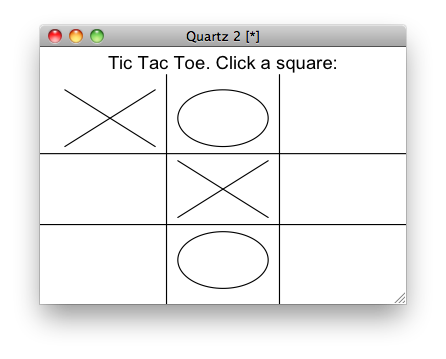
\includegraphics[width=.6\textwidth]{fig-basics-tic-tac-toe}
  \caption{Using a graphics device for a game of tic-tac-toe}
  \label{fig:basics-tic-tac-toe}
\end{figure}



In the above function \function{doPlay}, \function{clickHandler} is
an \defn{event handler}. Its job is to process the output of the
\function{locator} function, checking first if the user terminated
\function{locator} using the keyboard. If not it proceeds to draw the
move, and then, if necessary, the computer's move. Afterwards, play is
repeated until there is a winner or a ``cat's'' game.


\begin{Schunk}
\begin{Sinput}
 clickHandler <- function(iloc) {
   if(is.null(iloc)) 
     stop("Game terminated early")
   move <- floor(unlist(iloc))
   drawMove(move,"x")
   board[3*(move[2]-1) + move[1]] <<- 1
   if(!isFinished()) 
     doComputerMove()
   if(!isFinished()) 
     doPlay()
 }
\end{Sinput}
\end{Schunk}

The use of \verb+<<-+ in the handler illustrates a typical issue in
GUI design in \R.  User input changes the state of the application
through callback functions. These callbacks need to modify variables
\iprogram{variable scope}in some shared scope, which may be application-wide or specific to a
component. The lexical scoping rules of \R, i.e., nesting of closures,
has proven to be a useful strategy for managing GUI state. When this
is inconvenient, direct manipulation of environment objects is a
viable alternative. In the above case, we simply modify the global
environment, which encloses \function{clickHandler}.

%% validation of user input
\iprogram{validation}Validation of user input is an important task for a GUI. In the above,
the \function{clickHandler} function checks to see if the user
terminated the game early and issues a message.

%% Implement logic
At this point, we have a data model, a view of the model and the
logic that connects the two, but we still need to implement some of the
functions to tie it together.


This function draws either an ``x'' or an ``o''. It does so using the
\function{lines} function. The \code{z} argument contains the
coordinates of the square to draw.
\begin{Schunk}
\begin{Sinput}
 drawMove <- function(z,type="x") {
   i <- max(1,min(3,z[1])); j <- max(1,min(3,z[2]))
   if(type == "x") {
     lines(i + c(.1,.9),j + c(.1,.9))
     lines(i + c(.1,.9),j + c(.9,.1))
   } else {
     theta <- seq(0,2*pi,length=100)
     lines(i + 1/2 + .4*cos(theta), j + 1/2 + .4*sin(theta))
   }
 }
\end{Sinput}
\end{Schunk}

%% Resizing
One could use \code{text} to place a text ``x'' or ``o'', but this may
not scale well if the GUI is resized. Most GUI layouts allow for
\ilayout{resizing}dynamic resizing. This is necessary to handle the variety of data a
GUI will display. Even the labels, which one generally considers
static, will display different text depending on the language (as long
as translations are available).

%% JV: thanks
This function is used to test if a game is finished:
\begin{Schunk}
\begin{Sinput}
 isFinished <- function() {
   (any(abs(rowSums(board)) == 3) || 
    any(abs(colSums(board)) == 3) || 
    abs(sum(diag(board))) == 3 || 
    abs(sum(diag(apply(board, 2, rev)))) == 3)
 }
\end{Sinput}
\end{Schunk}
%
The matrix \code{m} allows us to easily check all the possible ways
to get three in a row.

This function picks a move for the computer:
\begin{Schunk}
\begin{Sinput}
 doComputerMove <- function() {
   newMove <- sample(which(board == 0),1) # random !
   board[newMove] <<- -1    
   z <- c((newMove-1) %% 3, (newMove-1) %/% 3) + 1
   drawMove(z,"o")
 }
\end{Sinput}
\end{Schunk}
%
The move is converted into coordinates using \code{\%\%} to get the
remainder and \code{\%/\%} to get the quotient when dividing an
integer by an integer. This function just chooses at random from the
left over positions; we leave implementing a better strategy to the
interested reader.

%% main equivalent
Finally, we implement the main entry point for our GUI:
\begin{Schunk}
\begin{Sinput}
 playGame <- function() {
   board <<- matrix(rep(0,9), nrow=3)  
   layoutBoard()
   doPlay()
   mtext("All done\n",1)
 }
\end{Sinput}
\end{Schunk}
%
When the game is launched, we first lay out the board and then call
\function{doPlay}. When \function{doPlay} returns, a message is written
on the screen.

This example adheres to the model-view-controller design pattern that
is implemented by virtually every complex GUI. We will encounter this
pattern throughout this book, although it is not always explicit.

%% endless tweak
For many GUIs there is a necessary trade-off between usability and
complexity. As with any software, there is always the temptation to
continually add features without regard for the long term cost. In
this case, there are many obvious improvements: implementing a better
artificial intelligence, drawing a line connecting three in a row when
there is a win, indicating who won, etc. Adding a feature adds
complexity to the interface, often useful, but sometime it just
increases the burden on the user.

\section{GUI Design Principles}
\label{sec:GUI:design}
% Section to introduce GUI design and principles through a comparison of
% three dialogs and general discussion


%% mac defs:

% Document windows contain file-based user data. They present a view
% into the content that people create and store. If the document is
% larger than the window, the window shows a portion of the document’s
% contents and provides users with the ability to scroll to other areas.

% Application windows are the main windows of applications that are not
% document-based. These windows can use the standard Aqua window look
% and features or (less frequently) the brushed metal look.

% Utility windows float above other windows and provide tools or
% controls that users can work with while documents are open. Utility
% windows (also called palettes) are discussed in more detail
% in “Utility Windows.” (page 202)

% Dialogs and alerts require a response from the user. These are
% discussed in “Dialogs.” (page 207)


The most prevalent pattern of user interface design is denoted WIMP,
which stands for Window, Icon, Menu and Pointer (i.e., mouse). The
WIMP approach was developed at Xerox PARC in the 1970's and later
popularized by the Apple Macintosh in 1984. This is particularly
evident in the separation of the window from the menu bar on the Mac
desktop. Other graphical operating systems, such as Microsoft Windows,
later adapted the WIMP paradigm, and libraries of reusable GUI
components emerged to support development of applications in such
environments. Thus, GUI development in R adheres to a WIMP approach.

The primary WIMP component from our perspective is the window. A
typical interface design consists of a \igui{top-level window}top-level window referred to as
the \dfnref{document window} that shows the current state of a
``document,'' whatever that is taken to be. In \R\/ it could be a data
frame, a command line, a function editor, a graphic or an arbitrarily
complex form containing an assortment of such elements. 

%% JV: control or "action" here?
%% ML: tried to make this clearer

Abstractly, WIMP is a command language, where the user executes
commands, often called actions, on a document by interacting with
graphical controls. Every control in a window belongs to some abstract
menu. Two common ways of organizing controls into menus are the
menu bar and toolbar.

The parameters of an action call, if any, are controlled in
sub-windows. These sub-windows are termed \dfnref{application windows}
by Apple~\footcite{APPLE:HIG}, but we prefer the term \igui{dialogs}\dfnref{dialogs},
or \dfnref{dialog boxes}. These terms may also refer to smaller
sub-windows that are used for alerts or confirmation. The program
often needs to wait for user input before continuing with an action,
in which case the window is modal. We refer to these as \dfnref{modal
  dialog boxes}.

Each window or dialog typically consists of numerous controls laid out
in some manner to facilitate the user interaction. Each window and
control is a type of \textit{widget}, the basic element of a
GUI. Every GUI is constituted by its widgets. Not all widgets are
directly visible by the user; for example, many GUI frameworks employ
invisible widgets to lay out the other widgets in a window.

There is a wide variety of available widget types, and widgets may be
combined in an infinite number of ways. Thus, there are often numerous
means to achieve the same goals. For example,
Figures~\ref{fig:GUI:print-dialogs} and \ref{fig:GUI:print-dialogs-R}
show three dialogs, representing typical dialogs from the three main
operating systems, that perform the same task -- collect arguments
from the user to customize the printing of a document. Although all
were designed to do the same thing, there are many differences in
implementation.

%% ML: Print dialogs might be problematic, especially with Firefox, which
%% (through GTK+) will use the platform native print dialog. On Linux,
%% there is no native dialog, so GTK+ implements one. This might not
%% be true of Firefox 2.0 specifically, but that is getting old
%% now. What about taking the print dialog from the R Windows GUI?

%% Principles of GUI layout
%% http://www.sylvantech.com/~talin/projects/ui_design.html has a nice list

\begin{figure}
  \centering
  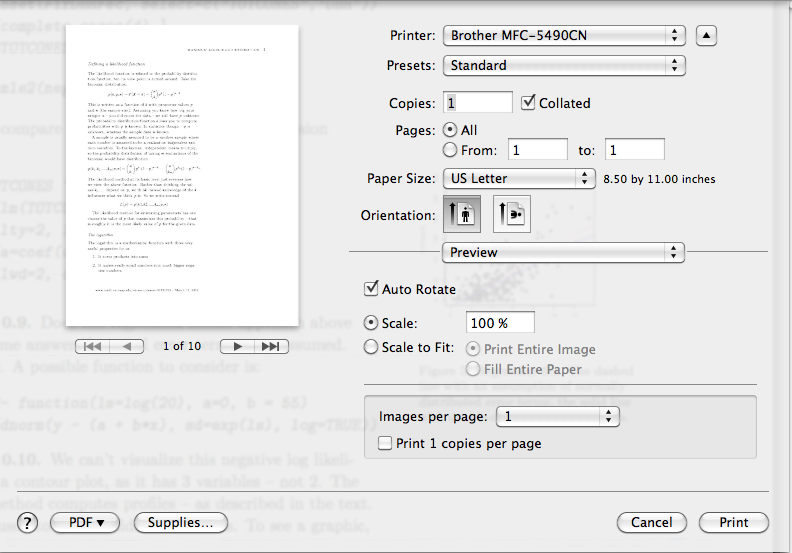
\includegraphics[width=.75\textwidth]{fig-mac-print}
   \\
   
  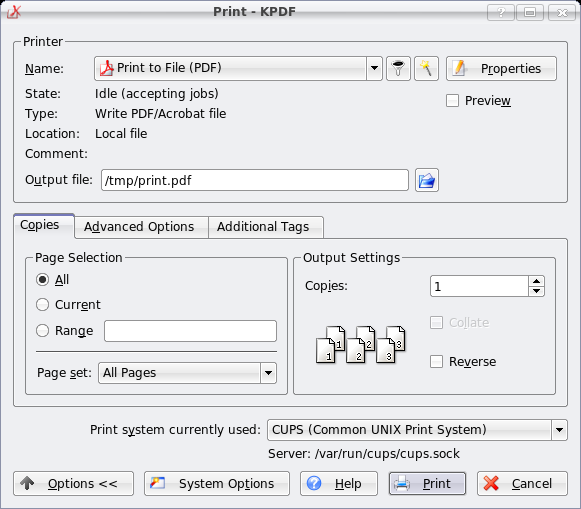
\includegraphics[width=.75\textwidth]{kde-print}
  \caption{Two print dialogs. One from Mac OS X 10.6 and one from KDE 3.5.}
  \label{fig:GUI:print-dialogs}
\end{figure}


\begin{figure}
  \centering
  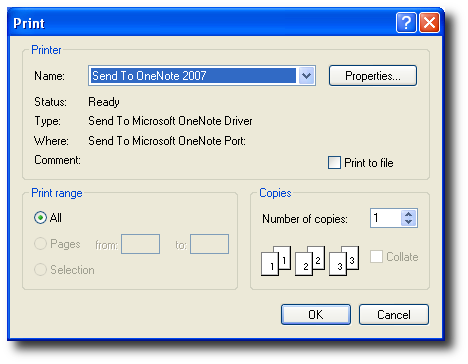
\includegraphics[width=.80\textwidth]{r-print-dialog}
  \caption{\R's print dialog under Windows XP using XP's native dialog.}
  \label{fig:GUI:print-dialogs-R}
\end{figure}

%% Choice of widget -- familiar metaphors, use of icons, 
In some cases, typical usage suggests one control over another. The
choice of printer for each is specified through a combo box. However,
for other choices a variety of widgets are employed. For example, the
control to indicate the number of copies for the Mac is a simple text
entry window, whereas for the KDE and Windows dialog it
is a spin button. The latter minimizes user error, say through entering
a non-positive integer. The KDE and Mac dialogs have icons to
compactly represent actions, whereas the the Windows example has none. The
landscape icon for the Mac is very clear and provides this feature
without having to use a sub dialog.


%% Choice of layout -- positioning, focus, use of spacing, center
%% balance, vs. ...
How the interfaces are laid out also varies.  All
panels are read top to bottom, although the Mac interface also has a very
nice preview feature on the left side. The KDE dialog uses frames to
separate out the printer arguments from the arguments that specify how
the print job is to proceed. The Mac uses a vertical arrangement to
guide the user through this. For the Mac, horizontal separators are
used instead of frames to break up the areas, although a frame is used
towards the bottom. Apple uses a center balance for its controls. They
are not left justified as are the KDE and Windows dialogs. Apple has
strict user-interface guidelines and this center balance is a design
decision.

%% feature exposure, Choice of options -- what to show, what to leave out
The layout also determines how many features and choices are visible to the
user at a given time.  For example, the Mac GUI uses ``disclosure
buttons'' to allow access to printer properties and the PDF settings,
whereas KDE uses a notebook container to show only a subset of the
options at once.

%% state visualization: sensitive/not; focus, not, 
The Mac GUI provides a very nice preview of the current document
indicating to the user clearly what is to be printed and how
much. Adjusting GUIs to the possible state is an important user
interface property.  GUI areas that are not currently sensitive to
user input are grayed out. For example, the ``collate'' feature of the
GUI only makes sense when multiple copies are selected, so the
designers have it grayed out until then. A common element of GUI
design is to only enable controls when their associated action is
possible, given the state of the application.

%% shortcuts -- default button, keyboard accelerators
 
The Mac GUI has the number of pages in focus, whereas Windows places
the printer in focus. This allows the user to interact with the GUI
without the mouse. Typically the \kbd{tab} key is used to step through
the controls. GUI's often have shortcuts that allow power users to
initiate actions or shift the focus directly to a specific widget
through the keyboard.  Most dialogs also have a default button, which
will initiate the dialog action when the \kbd{return} key is
pressed. The KDE dialog, for example, indicates that the ``print''
button is the default button through special shading.

%% help
% For such a common dialog, it is unlikely the user will need help. As
% such the Windows dialog does not provide a link. However, the
% KDE and Mac dialogs do. A dialog should provide assistance for
% complex and unfamiliar tasks.

%% safety -- postion of buttons
%% ML: Do we really want to mention something that is not applicable?
%% JV; Agreed
% The Apple human interface guidelines suggest putting buttons that can
% cause the destruction of data separate from other control buttons. As
% this isn't directly applicable here, we see that Apple does separate
% buttons that are common to many dialogs (cancel, print) from the ones
% specific to the dialog. The KDE buttons have nice icons, but their
% similar, but irregular, sizing is a bit unusual.


Each dialog presents the user with a range of buttons to initiate or
cancel the printing. The Windows ones are set on the right and consist
of the standard ``OK'' and ``Cancel'' buttons. The Mac interface uses
a spring to push some buttons to the left, and some to the right to
keep separate their level of importance. The KDE buttons do so as
well, although one can't tell from the image. However, one can see the use
of stock icons on the buttons to guide the user. 


%% JV should we leave this in? I'm wondering. We do it better in the
%% chapters perhaps
\section{Controls}
\label{sec:GUI:basic-components}
%% ML: This section and the next should probably be reorganized so
%% that they do a better job of referring to examples. Otherwise it
%% feels like we're stating a series of groundless generalities.

This section provides an overview of many common controls, i.e.,
widgets that either accept input, display data or provide visual
guides to help the user navigate the interface. If the reader is
already familiar with the conventional types of widgets and how they
are arranged on the screen, this section and the next should be
considered optional.


\subsection{Choice of control}
\label{sec:choice-widget}
%% real estate, type of data


\begin{table}
\centering
\label{tab:gui-design-widget-type}
\caption{Table of possible selection widgets by data type and size}
\begin{tabular}{@{}lp{0.35\textwidth}p{0.35\textwidth}@{}}
\toprule

Type of data&Single&Multiple\\
\midrule
Boolean&Checkbox, toggle button&-\\Small list&radio button group\newline combo box\newline list box&checkboxgroup\newline list box\\Moderate list&combo box\newline list box&list box\\Large list&list box, auto complete&list box\\Sequential&slider\ spin button&\\Tabular&table&table\\Hierarchical&tree&tree
\\ \bottomrule
\end{tabular}
\end{table}
A GUI is comprised of one or more widgets. The appropriate choice
depends on a balance of considerations.  For example, many widgets
offer the user a selection from one or more possible choices.  An
appropriate choice depends on the type and size of the information
being displayed, the constraints on the user input, and on the space
available in the layout. As an example,
Table~\ref{tab:gui-design-widget-type} suggests different types
of widgets used for this purpose depending on the type and size of
data and the number of items to select.
  

Figure~\ref{fig:GUI:spss-11-term-selection} shows several such
controls in a single dialog. A checkbox enables an intercept,
a radio group selects either full factorial or a custom
model, a combo box selects the ``sum of squares'' type, and a
list box allows for multiple selection from the available
variables in the data set. 




%% Metaphors, user base
For many \R\/ object types there are natural choices of widget. For
example, values from a sequence map naturally to a slider or spin
button; a data frame maps naturally to a table widget; or a list with
similar structure can map naturally to a tree widget. However, certain
\R\/ types have less common metaphors. For instance, a formula object
can be fairly complex. Figure~\ref{fig:GUI:spss-11-term-selection}
shows an SPSS dialog to build terms in a model. \R\/ power users may
be much faster specifying the formula through a text entry box, but
beginning \R\/ users coming to grips with the command line and the
concept of a formula may benefit from the assistance of a well
designed GUI. One might desire an interface that balances the needs of
both types of user, or the SPSS interface may be appropriate. Knowing
the potential user base is important.




\begin{figure}
  \centering
  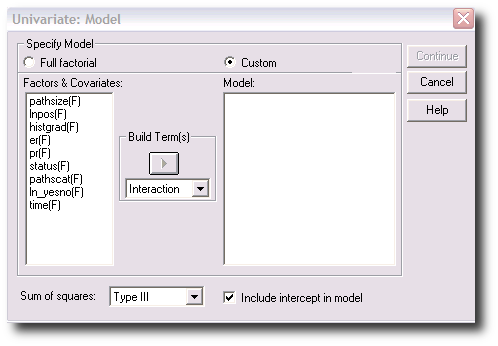
\includegraphics[width=.65\textwidth]{spss-11-formula-editor}
 \caption{A dialog box from SPSS version 11 for specifying terms
    for a linear model. The graphic shows a dialog that allows
    the user to specify individual terms in the model  using
    several types of widgets for selection of values, such as a radio button
    group, a checkbox, combo boxes, and list boxes. }
  \label{fig:GUI:spss-11-term-selection}
\end{figure}


\subsection{Presenting options}
\label{sec:GUI:basic-selection}

The widgets that receive user input need to translate that input into
a command that modifies the state of the application. Commands, like
\R{} functions, often have parameters, or options. For many options,
there is a discrete set of possible choices, and the user needs to
select one of them. Examples include selecting a data frame from a list of data
frames, selecting a variable in a data frame, selecting certain cases
in a data frame, selecting a logical value for a function argument,
selecting a numeric value for a confidence level or selecting a string
to specify an alternative hypothesis. Clearly there can be no
one-size-fits-all widget to handle the selection of a value.

% XXX REDO FIGURE
% \begin{figure}
%   \centering
%   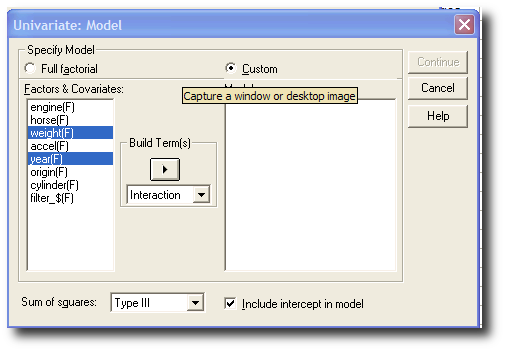
\includegraphics[width=.45\textwidth]{spss-11-model-selection}
%   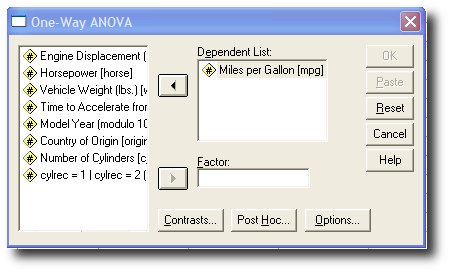
\includegraphics[width=.45\textwidth]{spss-11-one-way-anova}
%   \caption{Two dialog boxes from SPSS version 11 for specifying terms
%     for a linear model. The left graphic shows a dialog that allows
%     the user to specify individual terms in the model. This uses
%     several types of widgets for selection of values, such as a radio
%     group, a checkbox, combo boxes, and list boxes. The right graphic
%     shows a dialog that allows the user to specify response variables
%     and a grouping variable for a one-way ANOVA.}
%   \label{fig:GUI:spss-11-model-selection}
% \end{figure}


\subsubsection{Checkboxes}
\label{sec:GUI:checkboxes}

A \dfn{checkbox} specifies a value for a logical
(boolean) option. Checkboxes have labels to indicate which variable is
being selected. Combining multiple checkboxes into a group allows for
the selection of one or more values at a time.


\subsubsection{Radio buttons}
\label{sec:GUI:radio=button-groups}

A \dfn{radio button group} selects exactly one value from a vector of
possible values. The analogy dates back to old car radios where there
were a handful of buttons to select a preset channel. When a new
button was pushed in, the previously pressed button popped up.  Radio
button groups are useful, provided there are not too many values to
choose from, as all the values are shown. These values can be arranged
in a row, a column or both rows and columns to better fill the
available space. Figure~\ref{fig:GUI:ex-tcltk} uses radio button
groups for choosing the distribution, kernel and sample size for the
density plot.

\subsubsection{Combo boxes}
\label{sec:GUI:combo-boxes}

A \dfn{combo box} is similar to a radio button group, in that it is
used to select one value from several. However, a combo box only
displays the value currently selected, which reduces visual complexity
and saves space, at the cost of an extra click to show the
choices. Toolkits often combine a combo box with a text entry area for
specifying an arbitrary value, possibly one that is not represented in
the set of choices. A combo box is generally desirable over radio
buttons when there are more than four or five choices. However, the
combo box also has its limits. For example, some web forms require
choosing a country from a list of hundreds. In such cases, features
like incremental type ahead search are a common alternative.

\subsubsection{List boxes}

A \dfn{list box} displays a list of possible choices in a column.
While the radio button group and combo box select only a single value,
a list box supports multiple selection. Another difference is that the
number of displayed choices depends dynamically on the available
space. If a list box contains too many items to display them
simultaneously, a scrollbar is typically provided for adjusting the
visible range. Unlike the combo box, the choices are immediately visible
to the user.  Figure~\ref{fig:GUI:ex-tcltk} shows a list
box created by \R\/ that is called from the function
\command{chooseCRANmirror}. There are too many mirrors to fit on the
screen, but a combo box would not take advantage of the available
space. The list box is a reasonable compromise.

%% tcltk examples
\begin{figure}
  \centering
  \begin{minipage}[c]{.45\linewidth}
    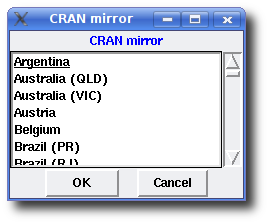
\includegraphics[width=1\textwidth]{ex-listbox}
  \end{minipage}
  \begin{minipage}[c]{.45\linewidth}
    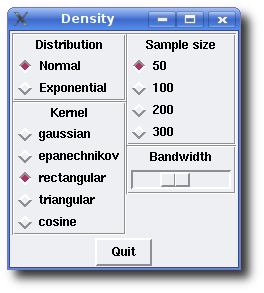
\includegraphics[width=1\textwidth]{tcltk-tkdensity}    
  \end{minipage}
 \caption{
    Two applications of the \pkg{tcltk} package. 
    %% 
    The left graphic is
    produced by \command{chooseCRANmirror} and uses a list box to
    allow selection from a long list of possibilities.
    %% 
    The right graphic is the \code{tkdensity} demo from the \pkg{tcltk}
    package. It uses radio buttons and a slider to select the
    parameter values for a density plot.
  }
  \label{fig:GUI:ex-tcltk}
\end{figure}

\subsubsection{Sliders and spin buttons}
\label{sec:GUI:sliders}

A \dfn{slider} is a widget that selects a value from a sequence of
possible values typically through the manipulation of a knob that
moves or ``slides'' along a line that represents the range of possible
values. 
%%Some toolkits (e.g. Java/Swing) only allow for the sequence to
%%have integer values.  
Some toolkits generalize beyond a numeric
sequence. The slider is a good choice for offering the user a
selection of ordinal or numerical parameter values. For example, the
letters of the alphabet could be a sequence. The \code{tkdensity} demo
of the \pkg{tcltk} package (Figure~\ref{fig:GUI:ex-tcltk}) uses a
slider to dynamically adjust the bandwidth of a density estimate.

A \dfn{spin button} plays a similar role to the slider, in that it
selects a value within a set of bounds. Typically, this widget is
drawn with a text box displaying the current value and two arrows to
increment or decrement the selection. The text box can usually be
edited directly.  A spin button has the advantage of using less screen
space, and directly entering a specific value, if known, is easier
than selecting it with a slider. One disadvantage is that the position
of the selected value within the range is not as obvious compared to
the slider. As a compromise, combining a text box with a slider is
possible and often effective. A spin button is used in the KDE print
dialog of Figure~\ref{fig:GUI:print-dialogs} to adjust the number of
copies.

\subsection{Initiating an action}

After the user has specified the parameters of an action, typically
by interacting with the selection widgets presented above, it comes time to
execute the action. Widgets that execute actions include the familiar
buttons, which are often organized into menubars and toolbars.

\subsubsection{Buttons}
\label{sec:GUI:buttons}

A \dfn{button} issues commands when invoked, usually via a mouse click.
In Figure~\ref{fig:GUI:print-dialogs}, the ``Properties'' button, when
clicked, opens a dialog for setting printer properties. The button
with the wizard icon also opens a dialog.  As buttons execute an
action, they are often labeled with a verb.~\footcite{APPLE:HIG} In
Figure~\ref{fig:GUI:spss-11-term-selection} we see how SPSS uses
buttons in its dialogs: buttons which are not valid in the current
state are disabled; buttons which are designed to open subsequent
dialogs have trailing dots; and the standard actions of resetting the
data, canceling the dialog or requesting help are given their own
buttons on the right edge of the dialog box.

To speed the user through a dialog, a button may be singled out as the
default button, so its action will be called if the user presses the
\kbd{return} key. Actions may be given shortcut bindings, and their
button proxies typically reflect the proper key combination to invoke
the action The KDE print dialog in Figure~\ref{fig:GUI:print-dialogs}
has these bindings indicated through the underlined letter on the
button labels.

%% ML: besides the accelerator comment, the below might be too much detail
%% JV: I'll leave it for the toolkit chapters if appropriate.
%% adjustments
% The look of the button can usually be manipulated.  A button is given
% a relief through its border, shading, and perhaps a color gradient
% along its face. Some toolkits allow these to be optionally drawn,
% thereby making a button look more like a label, as described below.
% The button text may have some markup or an indication of a accelerator
% keyboard binding, such as the \text{\underline{C}ontrasts...} button
% in the dialog shown in the right graphic of
% Figure~\ref{fig:GUI:spss-11-model-selection}.

\subsubsection{Icons}
\label{sec:GUI:icons}

In the WIMP paradigm, an \dfn{icon} is a pictorial representation of a
resource, such as a document or program, or, more generally, a
concept, such as a type of file. An application GUI typically adopts
the more general definition, where an icon is used to augment or
replace a text label on a button, a toolbar, in a list box, etc. When
icons appear on toolbars and buttons, they are associated with
actions, so an icon should be a pictorial representation of an
action.
% ML: too much detail?
% JV: agreed
% Except for the default installation of \pkg{tcltk}, images and icons
% may be specified in a variety of different formats.  Icons can come in
% several different sizes from 16 by 16 pixels to 128 by 128. For
% toolbars and menu bars, the toolkit takes care of selecting the
% appropriate icon.


\subsubsection{Menu Bars}
\label{sec:GUI:menubars}

Menus play a central role in the \acronym{WIMP} desktop. The \dfn{menu
  bar} contains items for many of the actions supported by the
application.  By convention, menu bars are associated with a top-level
window. This is enforced by some toolkits and operating systems, but
not all. In Mac OS X, the menu bar appears on the top line of the
display, but other platforms place the menu bar at the top of the
top-level window. In a statistics application, the ``document'' may be
viewed, for example, as the active data frame, a report, or a graphic.

The styles used for menu bars are fairly standardized, as this allows
new users to quickly orient themselves within a GUI. The visible menu
names are often in the order \code{File}, \code{Edit}, \code{View},
\code{Tools}, then application specific menus, and finally a
\code{Help} menu. Each visible menu item when clicked opens a menu of
possible actions. The text for these actions conventionally use a
\code{...}  to indicate that a subsequent dialog will open so that
more information can be gathered to complete the action. The text may
also indicate a key-board accelerator, such as \code{Find
  \underline{N}ext F3} indicating that both ``N'' as a keyboard
accelerator and F3 as a shortcut will initiate this same
action. (Shortcuts are not translated, but keyboard accelerators must
be. As such, their use is less so. In particular, keyboard
accelerators are not supported in Mac OS X menus.)

Not all actions will be applicable at any given time. It is
recommended that rather than deleting these menu items, they be
disabled, or grayed out, instead. %%~\ref{KDE:HIG}

Menus may come to contain many items. To help the user navigate, menu
items are usually grouped with either horizontal separators or
hierarchical submenus. %%The latter are indicated with an arrow.

The use of menus has evolved to also allow the user to set properties
or attributes of current state of the GUI. There may be checkboxes
drawn next to the menu item or some icon indicating the current state.

Another use of menus is to bind contextual menus (popup menus) to
certain mouse clicks on GUI elements. Typically right mouse clicks
will pop up a menu that lists often-used commands that are appropriate
for that widget and the current state of the GUI. In Mac OS X
one-button users, these menus are bound to a \kbd{control}-click.

\subsubsection{Toolbars}
\label{sec:GUI:toolbars}

Toolbars are used to give immediate access to the frequently used actions
defined in the menu bar. Toolbars typically have icons representing the
action and perhaps accompanying text. They traditionally appear on the
top of a window, but sometimes are used along the edges. 

%% Might not be the best place... any other options?
\subsubsection{Action Objects}
\label{sec:GUI:actions}

When clicking on a button, the user expects some ``action'' to
occur. For example, some save dialog is summoned, or some page is
printed.  GUI toolkits commonly represent such actions as formal,
invisible objects that are proxied by widgets, usually buttons, on the
screen.  Often, all of the primary commands supported by an
application have a corresponding action object, and the buttons
associated with those actions are organized into menu bars and
toolbars.

An action object is essentially a data model, with each proxy widget
acting as a view. Common components of an action include a textual
label, an icon, perhaps a shortcut, and a handler to call
when the action is selected.
%% JV this repeats the above
% When a particular action is not possible
% due to the state of the GUI, it should be disabled, so that the
% associated widgets are not sensitive to user interaction.


\subsection{Modal dialogs}
\label{sec:GUI:modal-dialogs}

A \dfnref{modal dialog box} is a dialog box that keeps the focus until
the user takes an action to dismiss the box. It prompts a user for
immediate input, for example asking for confirmation when overwriting
a file. Modal dialog boxes can be disruptive to the flow of
interaction, so are used sparingly. As the control flow is
blocked until the window is dismissed, functions that display modal
dialogs can return a value when an event occurs, rather than have a
handler respond to asynchronous input. The \command{file.choose}
function, mentioned below, is a good example. When called during an
interactive \R\/ session, the user is unable to interact with the
command line until a file has been specified or the dialog dismissed.

\subsubsection{Message dialogs}
\label{sec:GUI:message-dialogs}

A \dfnref{message dialog} is a high-level dialog widget for
communicating a message to the user. By convention, there is a small
rectangular box that appears in the middle of the screen with an icon
on the left and a message on the right. At the bottom is a button to
dismiss the dialog, often labeled ``OK.''  Additional
buttons/responses are possible. The \dfnref{confirmation dialog}
variant would add a ``Cancel'' button which invalidates the proposed
action.

\subsubsection{File choosers}
\label{sec:GUI:file-choosers}

A file chooser allows for the selection of files and directories. They
are familiar to any user of a GUI. A typical \R\/ installation has the
functions \command{file.choose} and \command{tkchooseDirectory} (in
the \pkg{tcltk} package) to select files and directories.

Other common choosers are color choosers and font choosers.

\subsection{Displaying data}
\label{sec:GUI:tabular-display}

Table and tree widgets support the display and manipulation of tabular
and hierarchical data, respectively. More arbitrary data
visualization, such as statistical plots, can be drawn within a GUI
window. All the toolkits we discuss have some means to embed \R's graphics.

%% JV: Need to include filtering example here

\subsubsection{Tabular display}

A \dfn{table widget} shows tabular data, such as a data frame, where
each column has a specific data type and cell rendering strategy.
Table widgets handle the display, sorting and selection of records
from a dataset. Depending on the configuration of the widget, cells
may be editable.  Figure~\ref{fig:GUI:spotfire} shows a table widget
in a Spotfire web player demonstration. 

\begin{figure}
  \centering
  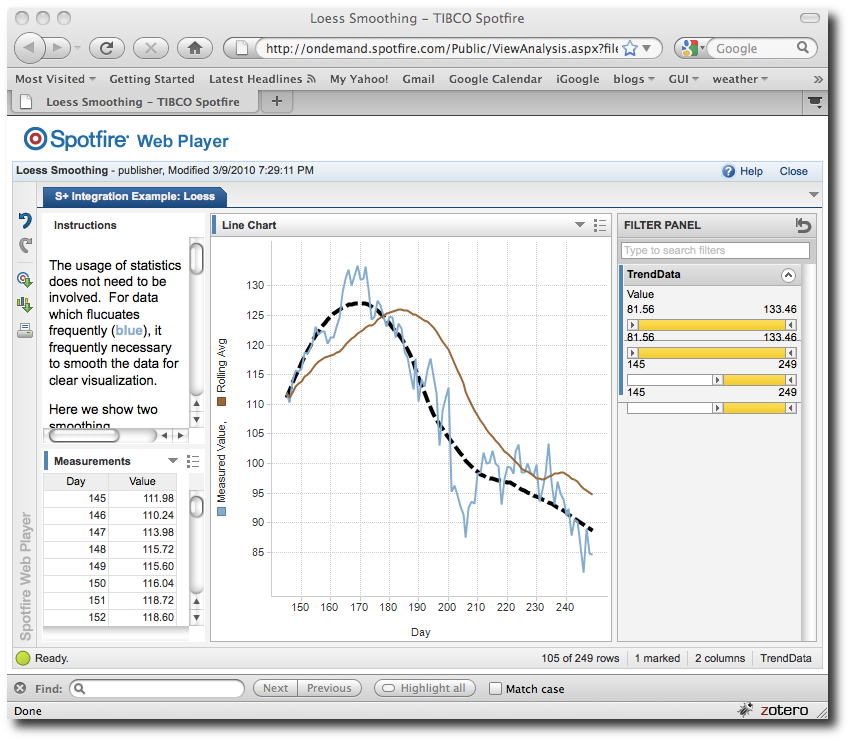
\includegraphics[width=0.8\textwidth]{fig-spotfire}
  \caption{A screen shot from Tibco's Spotfire web player illustrating
    a table widget (lower left), displaying the cases that are
    summarized in the graphic. The right bar filters the cases in the table. }
  \label{fig:GUI:spotfire}
\end{figure}


% \begin{figure}
%   \centering
% %%  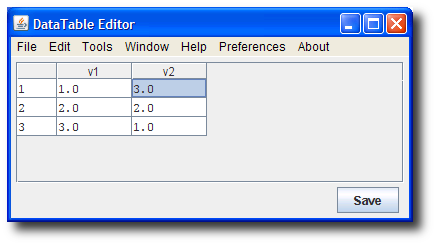
\includegraphics[width=.4\textwidth]{JGR-data-editor}
%   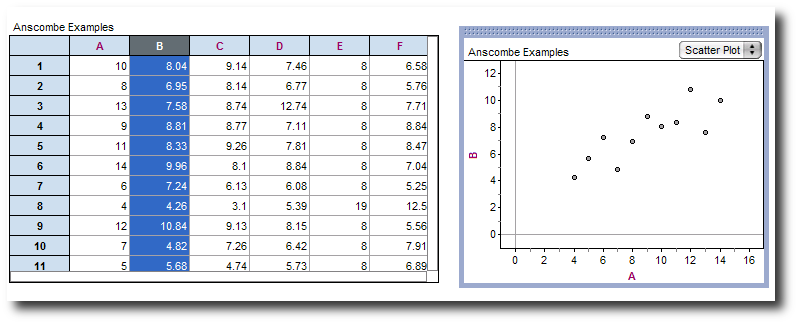
\includegraphics[width=.55\textwidth]{fathom-2-1-xyplot}
%   \caption{
%     Two windows showing the use of table widgets.
%     %%
    
% %     The left graphic shows the data editor from \pkg{JGR} using the
% %     table widget in Java.  
%     %%
%     The right graphic shows a data table and a graph in Fathom 2.1
%     with two views of the same data. One view uses a table widget, the
%     other a graph. Changes to one or the other views cause an update
%     to the underlying model. This model then will notify its various
%     displays to update. This arrangement allows for dynamic linking of
%     the table and the graph.}
%   \label{fig:GUI:table-widgets}
% \end{figure}

\subsubsection{Tree widgets}
\label{sec:GUI:tree-widgets}

So far, we have seen how list boxes display homogeneous vectors of
data, and how table widgets display tabular data, like that in a data
frame. Other widgets support the display of more complex data
structures. If the data has a hierarchical structure, then a \dfn{tree
  widget} may be appropriate for its display. Examples of hierarchical
data in \R\/ are directory structures, the components of a list, or
class hierarchies. The object browser in \pkg{JGR} uses a tree widget
to show the components of the objects in a users session
(Figure~\ref{fig:GUI:R-guis-exs-JGR}). The root node of the tree is
the ``data'' folder, and each data object in the global workspace is
treated as an offspring of this root node. For the data frame
\code{iraq}, its variables are considered as offspring of the data
frame. In this case these variables have no further offspring, as
indicated by the ``page'' icon.

%%%%%%%%%%%%%%%%%%%%%%%%%%%%%%%%%%%%%%%%%%%%%%%%%% 
\subsection{Displaying and editing text}
\label{sec:GUI:text-widgets}

The letter \acronym{P} in \acronym{WIMP} stands for ``pointer,'' so it
is unsurprising that \acronym{WIMP} GUIs are designed around the
pointing device. The keyboard is generally relegated to a secondary
role, in part because it is difficult to both type and move the mouse
at the same time. For statistical GUIs, especially when integrating
with the command-line interface of \R\/, the flexibility afforded by
arbitrary text entry is essential for any moderately complex
GUI. Toolkits generally provide separate widgets for text entry
depending on whether the editor supports a single line or multiple
lines.

\subsubsection{Single line text}
\label{sec:GUI:single-line-text}

A text entry widget for editing a single line of text is found in the
KDE print dialog (Figure~\ref{fig:GUI:print-dialogs}). It specifies
the page range. Specifying a complex page range, which might include
gaps, would require a complex point-and-click interface. In
order to avoid complicating the GUI for a feature that is rarely
useful, a simple language has been developed for specifying page
ranges. There is overhead involved in the parsing and validation of
such a language, but it is still preferable to the alternative.

\subsubsection{Text edit boxes}
\label{sec:GUI:textboxes}

Figure~\ref{fig:GUI:R-guis-exs-Rcmdr} shows three multi-line text
entries in an \pkg{Rcmdr} window. It provides an \R\/ console and
status message area. The ``Output Window'' demonstrates the utility of
formatting attributes. In this case, attributes specify the color of
the commands, so that the input can be distinguished from the output.



\begin{figure}
  \centering
  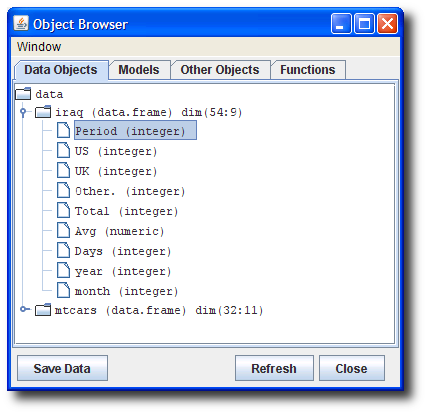
\includegraphics[width=.6\textwidth]{JGR-object-browser}
 \caption{
   The object browser in the \pkg{JGR} GUI
   using a tree widget 
   to display the possibly hierarchical nature of \R\/ objects.
   }
 \label{fig:GUI:R-guis-exs-JGR}
\end{figure}


\XXX{Not needed here?}
% %% A table showing the values and constructors
% %% Make changes to gnumeric spreadsheet, export
% {\small
% \newcommand{\PARASIZE}{1.25in}
% \newcommand{\LARGEPARASIZE}{1.45in}
% \begin{landscape}
%   \begin{table}[tbp]
%     \centering
%     \begin{minipage}{1.0\textwidth}
%       \begin{tabular}{lp{\PARASIZE}@{\quad}p{\LARGEPARASIZE}@{\quad}p{\PARASIZE}@{\quad}p{\PARASIZE}@{\quad}p{\PARASIZE}@{\quad}c}
%         %%
%         Widget & \code{gWidgets} & \code{RGtk2} & \code{RwxWidgets} &
%         \code{tcltk}~\footnote{Some constructors require add-on
%           libraries, as indicated by parentheses.} & \code{rJava} &\\
%         \hline
%         \SweaveInput{widgets-constructors}
%       \end{tabular}
%     \end{minipage}
%     \caption{A table listing several common widgets with a constructor for
%       different toolkits discussed in the text.}
% \label{tab:GUI:widgets-constructors}
%   \end{table}
% \end{landscape}
% }

%%%%%%%%%%%%%%%%%%%%%%%%%%%%%%%%%%%%%%%%%%%%%%%%%% 
\subsection{Guides and feedback}
\label{sec:GUI:info-display}

Some widgets display information but do not respond to user
input. Their main
purpose is to guide and the user through the GUI and to display
feedback and status messages.

\subsubsection{Labels}
\label{sec:GUI:labels}
%% Static Text
A label is a widget for placing text into a GUI that is typically not
intended for editing, or even selecting with a mouse. The main role of
a label is to describe another component of the GUI. Most toolkits
support rich text in labels. Figure~\ref{fig:GUI:R-guis-exs-Rcmdr}
shows labels marked in red and blue in \pkg{tcltk}.

\subsubsection{Statusbars}
\label{sec:GUI:statusbars}

A statusbar displays general status messages, as well as feedback on
actions initiated by the user, such as progress or errors. In the
traditional document-oriented GUI, statusbars are placed at the bottom.

Related to status bars are info bars or alert boxes, that allow a
programmer to leave a transient message for the user usually just
below the toolbar.

\subsubsection{Tooltips}
\label{sec:GUI:basic-tooltips}

A tooltip is a small window that is displayed when a user hovers their
mouse over a tooltip-enabled widget. These are an embellishment for
providing extra information about a particular piece of content
displayed by a widget. A common use-case is to guide new users of a
GUI. Many toolkits support the display of interactive hypertext in a
tooltip, which allows the user to request additional details.

\subsubsection{Progress bars}

A progress bar indicates progress on a particular task, which may or
may not be bounded. A bounded progress bar usually reports progress in
terms of percentage completed. Progress bars should be familiar, as
they are often displayed during software installation and while
downloading a file. For long-running statistical procedures they can
give useful feedback to the user that something is happening.

%% combined with modal dialogs
% \subsection{Choosers}
% \label{sec:GUI:choosers}

% Certain standard widgets are used to select values from a range
% defined by the system the user is on.


% \subsubsection{Color choosers}
% \label{sec:GUI:color-pickers}

% A color picker allows the selection of a color. 

% \subsubsection{Font choosers}
% \label{sec:GUI:font-choosers}

% A font chooser allows the selection of a font. 


\begin{figure}
  \centering
 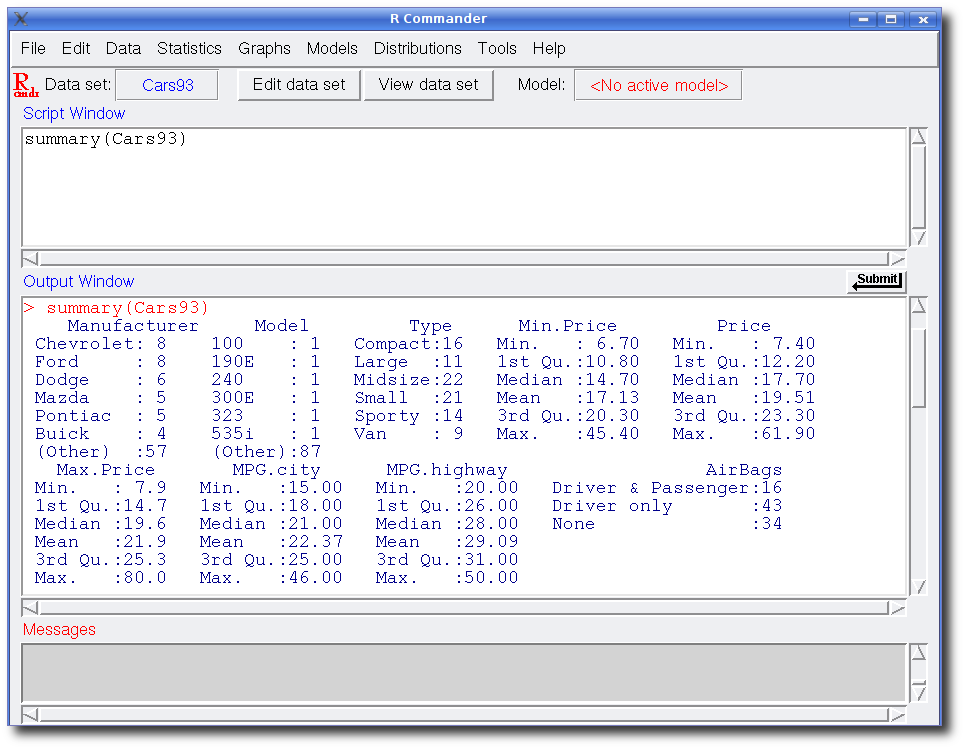
\includegraphics[width=.8\textwidth]{Rcmdr-main-window}
  \caption{
    Screenshot showing the main Rcmdr (1.3-11) window
    illustrating the use of multi-line text entry areas for a command
    area, an output area and a message area.}
  \label{fig:GUI:R-guis-exs-Rcmdr}
\end{figure}

\section{Containers}
\label{sec:GUI:basic-components-containers}
%% Containers

%%% FIXME: move to \paragraph{} instead of \subsubsection{}?

%% ML: Layout management is orthogonal to the type of container. This
%% is made obvious in the design of Swing and Qt: there is a separate
%% class hierarchy for layout managers, which are assigned to
%% container widgets. The container could be invisible or provide an
%% interface around its children, as with a frame, notebook or top-level
%% window. Thus, in Qt, a frame container could lay out its children
%% as a box, a grid, etc. I suggest discussing container types first,
%% and then discuss layout management policies, explaining that some
%% toolkits have widgets specific to a particular policy (and so
%% require a lot of nesting), while in others any container type is
%% capable of any type of layout.


%% JV: good point. 
% Widgets are arranged in a window to produce a GUI. Container widgets
% manage the layout. The simplest containers are like boxes
% that get packed in left to right or top to bottom. These boxes may be
% decorated with a frame or label, or may have some means of being
% hidden or displayed by the user. The nesting of box containers can
% provide a great deal of flexibility, but usually not
% enough. An example of a more flexible layout strategy is to position
% widgets on a grid.

%% Widget Hierarchy

The KDE print dialog of Figure~\ref{fig:GUI:print-dialogs} contains
many of the widgets we discussed in the previous section. Before we
can create such a dialog, we need to introduce how to position widgets
on the screen. This process is called \textit{widget layout}.

\ilayout{widget hierarchy}
A layout emerges from the organization of the widgets into a
hierarchy, where a parent widget positions its children within its
allocated space.  The top-level window is parentless and forms the
root of the hierarchy. A parent visually contains its children and
thus is usually called a \defn{container}. This design is natural,
because almost every GUI has a hierarchical layout. It is easy to
apply a different layout strategy to each region of a GUI, and when a
parent is added or removed from the GUI, so are its children.

It is sometimes tempting for novices to simply assign a fixed position
and dimensions for every widget in a GUI. However, such static layouts
do not scale well to changes in the state of the application or simply
changes to the window size dictated by the window manager. Thus, it is
strongly encouraged to delegate the responsibility of layout to a
\defn{layout manager} that dynamically calculates the layout as
constraints change. Depending on the toolkit, the layout manager might
be the container itself, or it might be a separate object to which the
container delegates.

Regardless, the type of layout is generally orthogonal to the type of
container. For example, a container might draw a border around its
children, and this would be independent of how its children are laid
out.  The rest of this section is divided into two parts: container
widgets and layout algorithms. We will continually refer back to the
KDE print dialog example as we proceed.

% The Apple guidelines\footcite[Ch. 15]{APPLE:HIG} suggest using ``center
% equalization'' for arranging widgets within a window. This means that
% the visual weight is balanced between the right and left side of the
% content area. This is not the case with the KDE print dialog.

\subsection{Containers}
\label{sec:containers}

\subsubsection{Top level windows}
\label{sec:GUI:top-level-windows}

The top-level window of a GUI is the root of the container
hierarchy. All other widgets are contained within it.  The
conventional main application window will consist of a menu bar, a
tool bar and a status bar. The primary content of the window is
inserted between the tool bar and the status bar, in an area known as
the \dfnref{client area} or \dfnref{content area}. In the case of a
dialog, the content usually appears above a row of buttons, each of
which represent a possible response. The print dialog conforms to the
dialog convention. The print options fill the content area, and there
is a row of buttons at the bottom for issuing a response, such as
``Print''.

A window is typically decorated with a title and buttons to iconify,
maximize, or close. In the case of the print dialog, the top-level
window is entitled ``Print -- KPDF.''. Besides the text of the title,
the decorations are generally the domain of the window manager (often
part of the operating system). The application controls the contents
of the window.

Once a window is shown, its dimensions are managed by the user,
through the window manager. Thus, the programmer must size the window
before it becomes visible. This is often referred to as the
``default'' size of the window. Positioning of a top-level window is
generally left to the window manager.

The top-level window forwards window manager events to the
application. For example, an application might listen to the window
close event in order to prompt a user if there are any unsaved changes
to a document.

% Table~\ref{tab:GUI:containers-constructors} lists them
% together and provides the constructor name for the different toolkits
% discussed in this book.

\subsubsection{Frames}
\label{sec:GUI:frames}

A frame is a simple container that draws a border, possibly with a
label, around its child. The purpose of a frame is to enhance
comprehension of a GUI by visually distinguishing one group of
components from the others. The displayed page of the notebook in
Figure~\ref{fig:GUI:print-dialogs} contains two frames, visually
grouping widgets by their function: either \code{Page Selection}
or \code{Output Settings}.

\subsubsection{Tabbed notebooks}
\label{sec:GUI:notebooks}

A notebook represents each of its children as a page in a notebook. A
page is selected by clicking on a button that appears as a tab. Only a
single child is shown at once. The tabbed notebook is a space
efficient, categorizing container that is most appropriate when a user
is only interested in one page at a time. Modern web browsers take
advantage of it to allow several web pages to be open at once within
the same window. In the KDE print dialog, detailed options are
collapsed into a notebook in order to save space and organize the
multitude of options into simple categories: ``Copies'', ``Advanced
Options'', and ``Additional Tags''.

% %% A table showing the values and constructors
% %% Make changes to gnumeric spreadsheet, export
% {\small
% \newcommand{\PARASIZE}{1.25in}
% \begin{landscape}
%   \begin{table}
%     \centering
%     \caption{A table listing several containers with a constructor for the
%     different toolkits discussed in the text.}
%     \begin{tabular}{lp{\PARASIZE}@{\quad}p{\PARASIZE}@{\quad}p{\PARASIZE}@{\quad}p{\PARASIZE}@{\quad}p{\PARASIZE}@{\quad}c}
%       Widget & \code{gWidgets} & \code{RGtk2} & \code{RwxWidgets} &
%       \code{tcltk} & \code{rJava} &\\
%       \hline
%       \SweaveInput{containers-constructors}
%     \end{tabular}
%     \label{tab:GUI:containers-constructors}
%   \end{table}
% \end{landscape}
% }


\subsubsection{Expanding boxes}
\label{sec:GUI:expanding-boxes}

An expanding container, or box, will show or hide its children, according to the
state of a toggle button. By way of analogy, radio buttons are to
notebooks as check buttons are to expanding containers. An expanding box
allows the user to adapt a GUI to a particular use case or mode of
operation. Often, an expanding box contains so-called ``advanced''
widgets that are only occasionally useful and are only of interest to
a small subset of the users. For example, the \code{Options} button in
Figure~\ref{fig:GUI:print-dialogs} controls an expanding box that
contains the print options, which are usually best left to their
defaults.

\subsubsection{Paned boxes}
\label{sec:GUI:paned-boxes}

Usually, a layout manager allocates screen space to widgets, but
sometimes the user needs to adapt the allocation, according to a
present need. For example, the user may wish to increase the size of
an image to see the fine details. The \dfnref{paned container}
supports this by juxtaposing panes, either vertically (stacked) or
horizontally. The area separating the panes, sometimes called a
\dfnref{sash}, can be adjusted by the user with the mouse.
   
\subsection{Layout algorithms}
\label{sec:GUI:layout}

\subsubsection{Box layout}
\label{sec:GUI:Box-containers}

\ilayout{box layout}The box layout is the most common type of layout algorithm for
positioning child components. A box will pack its children either
horizontally or vertically~\footnote{The \code{pack} command of
  \pkg{tcltk} can mix the two directions}. Usually, the widgets are
packed from left to right, for horizontal boxes, or from top to
bottom, in the case of a vertical box.  The upper left figure in
Figure~\ref{fig:GUI:box-possibilities} illustrates these possibilities.

\ilayout{resizing}The box layout needs to allocate space to its children in both the
vertical and horizontal directions. The typical box layout algorithm
begins by satisfying the minimum size requirements of its
children. The box may need to request more space for itself in order
to meet the requirement. 

Once the minimum requirements are satisfied, it is conventional and
usually desirable for the widgets to fill the space in the direction
orthogonal to the packing. For example, widgets in a horizontal box
will fill all of their vertical space (the upper right graphic in
Figure~\ref{fig:GUI:box-possibilities} shows some fill
possibilities). When this is not desired, most box widgets support
different ways of vertically (or horizontally) aligning the widgets
(the lower left graphic in Figure~\ref{fig:GUI:box-possibilities}).

More complex logic is involved in the allocation of space in the
direction of packing. Any available space after meeting minimum
requirements needs to be either allocated to the children or left
empty. This depends on whether any children are set to expand. The
available space will be distributed evenly to all expanding
children. Each child may fill that space or leave it empty. The
non-expanding children are simply packed against their
side of the container. If there are no expanding children, the
remaining space is left empty in the middle (or end if there are no
widgets packed against the other side). See the lower right
panel in Figure~\ref{fig:GUI:box-possibilities}. One could think
of this space being occupied by an invisible \ilayout{spring}spring. Invisible
expanding widgets also act as springs.


\begin{figure}
  \centering
  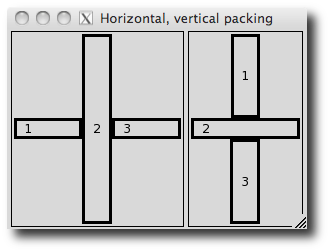
\includegraphics[width=.40\textwidth]{fig-basics-hor-ver}
  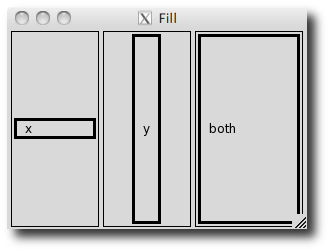
\includegraphics[width=.40\textwidth]{fig-basics-fill}\\
  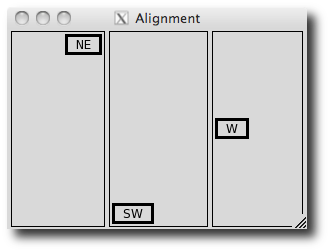
\includegraphics[width=.40\textwidth]{fig-basics-alignment}
  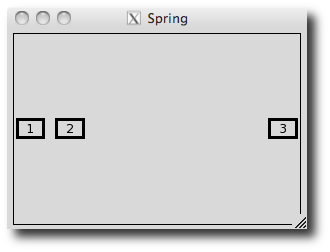
\includegraphics[width=.40\textwidth]{fig-basics-spring}
  \caption{
   %% 
    Different possibilities for packing child components within
    a box. 
    %% 
    The upper left shows horizontal and vertical layout.
    %% 
    The upper right shows some possible alignments or anchorings.
    %% 
    The lower left shows that a child could ``expand'' to fill the space
    either horizontally, vertically, or both.
    %% 
    The lower right shows both a fixed amount of space between the
    children and an expanding spring between the child components.  }
  \label{fig:GUI:box-possibilities}
\end{figure}

The button box in the KDE print dialog shows five buttons as child
components. At first glance the sizing appears to show that each
button is drawn to fully show its label with some fixed space placed
between the buttons. If the dialog is expanded, it is seen that there
is a spring between the 3rd and 4th buttons, so that the first 3 are
aligned with the left side of the window and the last two the right
side.

\subsubsection{Grid layout}
\label{sec:GUI:grid-layout}

The box layout algorithm only aligns its children along a single
dimension. The horizontal box, for example, vertically aligns its
children. Nevertheless, nesting permits the construction of complex
layouts using only simple boxes. However, it is sometimes desirable to
align widgets in both dimensions, i.e., to lay them out on a
\ilayout{grid layout}grid. The
most flexible grid layout algorithms allow non-regular sizing of rows
and columns, as well as the ability for a widget to span multiple
cells. Usually, a widget fills the cells allocated to it, but if this
is not possible, it may be anchored at a specific point within their
cell. 

The widgets in the ``Printer'' frame of
Figure~\ref{fig:GUI:box-possibilities} are subject to a grid layout
with five columns and six rows. The first row begins with the
``Name:'' label, and each widget in that row occupy a separate
column. This exposes the size of each column. The first column has
only labels, with text justified to the left.  The labels are aligned
horizontally to each other and vertically with adjacent field.


% \section{End of chapter notes}
% \label{sec:GUI:end-of-chapter}
% \XXX{ fill this in }

% More documentation on GUIs is available in book format or online. 

% For \GTK\/ there is the gtk tutorial (pygtk); GTK API; DTL's notes; example
% code in the \pkg{RGtk2} package; php-gtk cookbook

% For \wxWidgets the book; DTL omegahat pages; wxWidgets API;

% For \tcltk\/ ActiveStates API; wettenhall examples (sciviews);
% Dalgaard's papers; R mailing list; book

% For \Java\/ Sun's website tutorials; API; rJava package page; 

% Event loops




%%%%%%%%%%%%%%%%%%%%%%%%%%%%%%%%%%%%%%%%%%%%%%%%%%





%% R functions, practices for GUI programmng
\chapter{R Programming Practices for GUIs}
\label{chap:programming-practices}
%%%
\section{Why program GUIs in \R?}
\label{sec:GUIsInR}
%% place to discuss why program GUIs in R


\XXX{Cover these}
\begin{itemize}
\item Benefit to user of code -- complexity
\item Convenience
\item Reasonable speed, power
\item many options: RGtk2, tcltk, RPad, rJava, RwxWidgets, DTL stuff
\item Cross platform
\end{itemize}


%%
\section{Object Oriented Programming in \R}
\label{sec:OOP}
%% Object oriented programming in R

\subsection{Principles of object oriented programming}
\label{sec:princ-object-orient}

\subsubsection{Generic functions and methods in R}
\label{sec:gener-funct-meth}



\subsection{S3 Style}
\label{sec:PROG:S3}


 
% S3
% class(), dispatch, ``inheritance''
% use current generics
% define new generics
% not class based -- object based (MMaechler, but what does it mean?)




% -------------
% proto
% environments: \$, [, like a list; but passed through to functions,
%  unlike lists 
% <<>>=
% library(proto)
% f = function(obj) obj[['new']]<-"new"
% p = proto(); p$new = "old"; q = p$proto()
% e = environment(); e$new="old"
% l = list(); l$new = "old"
% f(q); f(e); f(l); print(c(q$new, p$new, e$new, l$new))
% @ 
% parents share properties with children -- not the other way. Why?
% child\$new looks in the enviroment of child for "new", if it is not
% found then it looks in enviroment of parent where it is found. This is
% broken when the child defines a property or method of that name.

% override dollar sign
% get/assign
% ex: ex-UndoRedo support: 

% ex: issue with overriding \$, (nextMethod) -- do that

% %%


\subsection{S4 Style}
\label{sec:PROG:S4}

% ----------------
% S4
% dispath -- multiple arguments
% defining classes, get classes, inheritance
% method signature
% use current methods
% add new methods
% promote  S3 object to S4 object


\section{Programming Issues when programming GUIs}
\label{sec:ProgrammingIssues}

\subsection{Pass by copy}
\label{sec:pass-by-copy}

\XXX{issues with modifying values in callback, double arrow
  assignement, assign, etc.}

\subsubsection{Variable lookup: Scoping}
\label{sec:vari-look-scop}

\subsubsection{Environments in \R}
\label{sec:environements-r}



\subsection{Converting text into \R\/ commands and \R\/ commands to text.}
\label{sec:text-to-R}
\XXX{eval(parse), do.call, ...}

\XXX{deparse, dput, sys.call, serialization}


\subsection{Efficient programming in \R}
\label{sec:efficient-programming}
\XXX{do.call, apply functions,...}
  
  
\subsection{Localization}
\label{sec:localization}

\XXX{gettext, etc.}



* nargs ..1 working with function args

* stringToObject: get, eval(parse(text=...)), do.call, match.fun,
serialize methods? assign, expressions?


\XXX{hash package  for global environment}




%% gWidgets
%%\part{The \pkg{gWidgets} package}
\label{chap:gWidgets-intro}
%% Put these somewhwere:

\XXX{use svalue(g), spacing to give some breathing room in a ggroup}

\XXX{something like ggroup(cont=w,spacing=10); svalue(g)=10}

\XXX{include listing data frame, listing variables by type}

\XXX{relationship with the toolkits

\XXX{getToolkitWidget, add method, ... only with RGtk2 (rJava?), only some widgets}}



%% gWidgets introduction
 
\newcommand{\ONLYIN}[1]{[only in #1]}

\chapter{\pkg{gWidgets}: Overview}
\label{sec:overview}

%% Overview of gWidgets

% ML: do we really want to discuss the unsupported rJava backend?
% I am also confused about gWidgetsWWW - is it an implementation or
% something that just resembles the gWidgets API?

% JV, I will drop rJava, put in gWidgetsQt, and make brief mention of gWidgetsWWW

The \pkg{gWidgets} package provides a toolkit-independent interface
for the \R\/ user to program graphical user interfaces from within
R. Although the package provides much less functionality than using a
native toolkit interface, \pkg{gWidgets} can be used to create
moderately complex GUIs quickly and easily using a programming
interface that is simpler and more familiar to the \R\/ user.

 
The \pkg{gWidgets} package started as a port to \pkg{RGtk2} of the
\pkg{iWidgets} interface, initially implemented only for Swing through
\pkg{rJava}~\citep{iWidgets}. The \pkg{gWidgets} package enhances that
original interface in terms of functionality and implements it for
multiple toolkits.  

% ML: should these two pieces be split?
\section{Installation, toolkits}
\label{sec:installation}

The \pkg{gWidgets} package is installed and loaded as other \R\/
packages that reside on CRAN. This can be done through the function
\code{install.packages} or in an \R\/ graphical front-end through a
dialog called from the menu bar. The \pkg{gWidgets} package only provides
the application programming interface (API). To actually create a GUI, one
needs to have: 
\begin{enumerate}
\item An underlying toolkit library. This can be either the \Tk\/
  libraries, the \Qt\/ libraries or the \GTK\/ libraries. The
  installation varies for each and depends on the underlying operating system.
  
\item An underlying \R\/
package that provides an interface to the libraries. The \pkg{tcltk}
package is a recommended pacakge for \R\/ and comes with the \R\/
software itself, the \pkg{RGtk2} and \pkg{Qt} packages may be installed
through \R's package management tools.
\item a \pkg{gWidgetsXXX} package to link \pkg{gWidgets} to the \R\/
  package. As of this writing, there are basically three such packages
  \pkg{gWidgetsRGtk2}, \pkg{gWidgetsQt} and \pkg{gWidgesttcltk}.  The
  \pkg{gWidgetsWWW} package is an independent implementation for web
  programming that is more or less faithful to the API, but not
  commented on further in this chapter.

\end{enumerate}

Not all features of the API are available in each package.  The help
pages in the \pkg{gWidgets} package describe the API, with the help pages in the
toolkit packages indicating differences or omissions from the API. For
the most part, the omissions are gracefully handled by simply
providing less functionality. We make note of major differences here,
realizing that over time they may may be resolved. Consult the package
documentation if in doubt.

Figure~\ref{fig:gWidgets-three-oses} shows how the same GUI code
can be rendered differently depending on the OS and the
toolkit. 

%%Figure~\ref{fig:gWidgetsWWW-same-gui} shows a similar GUI
%%using \pkg{gWidgetsWWW}.

XXX      [insert Qt graphics here] 
\begin{figure}
  \centering
  \begin{tabular}{ll}
     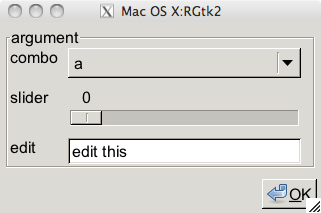
\includegraphics[width=0.45\textwidth]{ex-33-macosx-rgtk2} &
     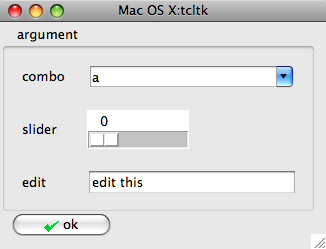
\includegraphics[width=0.45\textwidth]{fig-gWidgets-ex-33-tlctk}\\
    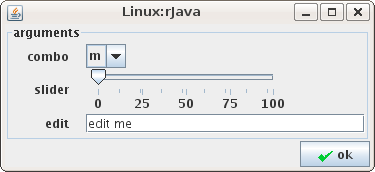
\includegraphics[width=0.45\textwidth]{ex-33-linux-rJava} &
     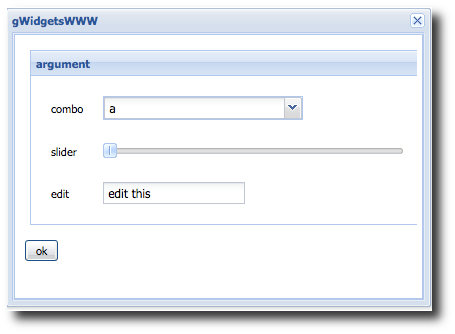
\includegraphics[width=0.45\textwidth]{ex-33-gWidgetsWWW}
 \end{tabular}
 \caption{The \pkg{gWidgets} package works with different operating
   systems and different GUI toolkits. This shows, the same code using the
   \pkg{RGtk2}, \pkg{tcltk}, \pkg{qtbase} packages for a toolkit. Additionally,
   the \pkg{gWidgetsWWW} package is used in the lower right figure.}
  \label{fig:gWidgets-three-oses}
\end{figure}

% %% Make figure -- work on layout here
% \XXX{Do mac, windows}
% \begin{figure}
%   \centering
%   \begin{tabular}{lccc}
%     & \pkg{RGtk2} & \pkg{tcltk} & \pkg{rJava} 
%     \\
%     L &
%     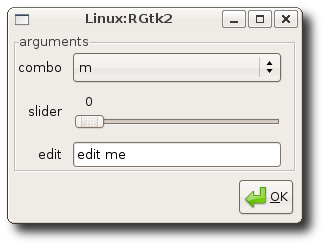
\includegraphics[width=0.3\textwidth]{ex-33-linux-rgtk2.png} &
%     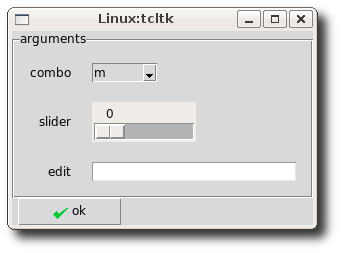
\includegraphics[width=0.3\textwidth]{ex-33-linux-tcltk} &
%     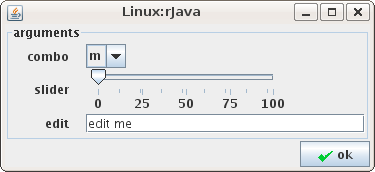
\includegraphics[width=0.3\textwidth]{ex-33-linux-rJava} 
%     \\
%     W &
%     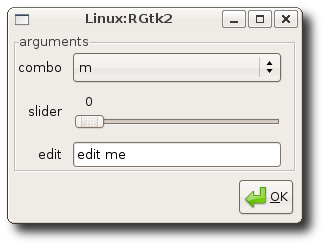
\includegraphics[width=0.3\textwidth]{ex-33-linux-rgtk2} &
%     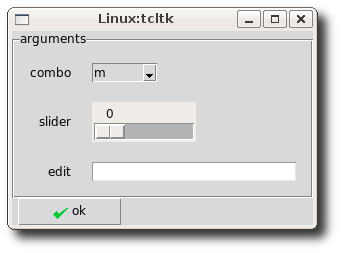
\includegraphics[width=0.3\textwidth]{ex-33-linux-tcltk} &
%     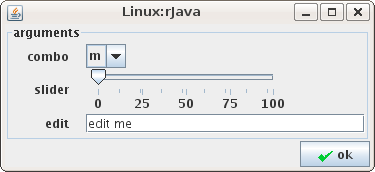
\includegraphics[width=0.3\textwidth]{ex-33-linux-rJava} 
%     \\
%     Mac &
%     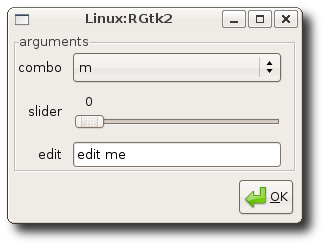
\includegraphics[width=0.3\textwidth]{ex-33-linux-rgtk2} &
%     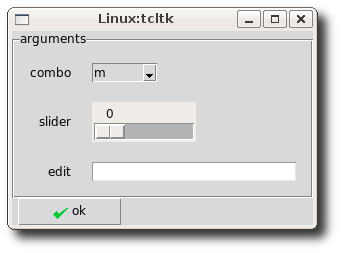
\includegraphics[width=0.3\textwidth]{ex-33-linux-tcltk} &
%     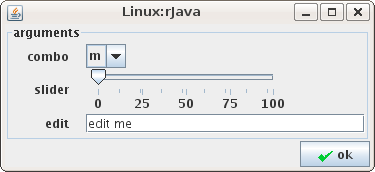
\includegraphics[width=0.3\textwidth]{ex-33-linux-rJava}
%   \end{tabular}
%   \caption{The \pkg{gWidgets} package works with different operating systems and different GUI toolkits. This shows the combination of \code{linux}, \code{Mac OS X (10.5)} and \code{Windows XP} and the packages \pkg{RGtk2}, \pkg{tcltk}, and \pkg{rJava}}
%   \label{fig:three-oses-three-toolkits}
% \end{figure}


% \begin{figure}
%   \centering
%   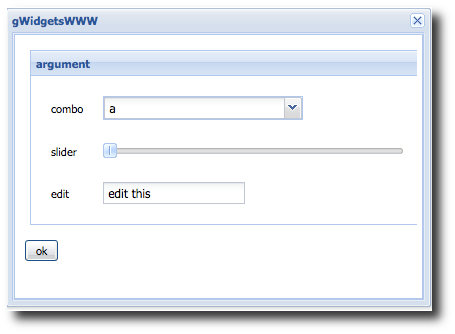
\includegraphics[width=.45\textwidth]{ex-33-gWidgetsWWW}
%   \caption{A GUI shown using \pkg{gWidgetsWWW}.}
%   \label{fig:gWidgetsWWW-same-gui}
% \end{figure}


\section{Startup}
%% starting package
The \pkg{gWidgets} package is loaded as other \R\/ packages:
\begin{Schunk}
\begin{Sinput}
 require(gWidgets)
\end{Sinput}
\end{Schunk}

A toolkit package is loaded when the first command is issued. If a
user does not have a toolkit installed, a message instructs the user
to install one.

%% Choice of toolkit
If a user has exactly one toolkit package installed, then that will be
used. But it is possible for more than one to be installed, in which
case the user is prompted to choose one through an interactive menu. This
choice can be avoided by setting the option \args{guiToolkit} to the
\code{XXX} in a \pkg{gWidgestXXX} package name, e.g.,
\begin{Schunk}
\begin{Sinput}
 options("guiToolkit"="RGtk2")
\end{Sinput}
\end{Schunk}

Although in theory the different toolkits can be used
together, in practice the different event loops created by each often
lead to issues that can lockup the \R\/ process.


\begin{example}{A first GUI}{eg:gWidgets:first-gui}
  As a first illustration of the use of \pkg{gWidgets}, a
  simple ``hello world'' type GUI can be produced through:
\begin{Schunk}
\begin{Sinput}
 w <- gwindow("Hello world example")
 b <- gbutton("Click me for a message", container=w)
 addHandlerClicked(b, handler=function(h,...) {
   print("Hello world")
   dispose(w)
 })
\end{Sinput}
\end{Schunk}
\end{example}

\section{Constructors}
\label{sec:constructors}
%% constructors
GUI objects are produced by constructors. In
Example~\ref{eg:gWidgets:first-gui} a top-level window and button
constructor were called. In
\pkg{gWidgets} most constructors have the following form: 
\begin{Schunk}
\begin{Sinput}
 gname(arguments, handler = NULL, action = NULL, 
       container = NULL,...,toolkit=guiToolkit())
\end{Sinput}
\end{Schunk}
where the \code{arguments} vary depending on the object being made. 

% ML: it seems strange to document so much of the design of gWidgets
% as the return value of a constructor

% removed section header. 

In addition to creating a GUI object, a constructor also returns a
useful \R\/ object. Except for modal dialog constructors, this is an
S4 object of a certain class containing two components: \code{toolkit}
and \code{widget}. The \code{toolkit} can be specified at time of
construction allowing tookits, in theory, to be mixed. Otherwise, the
\code{guiToolkit} function returns the currently selected toolkit, or
queries for one if none is selected.

% point about dispatch

Constructors dispatch on the \code{toolkit} value to call the
appropriate constructor in the toolkit implementation. The return
value from the toolkit's constructor is kept in the \code{widget}
component.  Generic methods have a double dispatch when called. The
first dispatch is based on the \code{toolkit} value and the method
calls a second generic, implemented in the toolkit-specific package,
with the same name as the first generic, except prefixed by a period
(\code{svalue} calls \code{.svalue}). The tookit generic then
dispatches based on the class of the \code{widget} argument and
perhaps other arguments given to the generic. The actual class of the
S4 object returned by the first constructor is (mostly) not
considered, but when we refer to methods for an object, we gloss over
this double dispatch and think of it as a single dispatch. This design
allows the toolkit packages the freedom to implement their own class
structure.

%% methods 
As with most \R\/ objects, one calls generic functions to
interact programatically with the object. Depending on the class, the
\pkg{gWidgets} package provides methods, for the
familiar S3 generics \generic{[}, \generic{[$<$-}, \generic{dim},
\generic{length}, \generic{names}, \generic{names$<$-},
\generic{dimnames}, \generic{dimnames$<$-}, \generic{update}.

In addition, \pkg{gWidgets} provides the new generics listed in
Table~\ref{tab:gWidgets-methods}.  These new generics provide a means
to query and set the primary value of the widget (\meth{svalue},
\meth{svalue\ASSIGN}), and various functions to effect the display of
the widget (\meth{visible\ASSIGN}, \meth{font\ASSIGN},
\meth{enabled\ASSIGN}, \meth{focus\ASSIGN}). The methods \meth{tag}
and \meth{tag\ASSIGN} are implemented to bypass the pass-by-copy
issues that can make GUI programming awkward at times.


%% insufficiency of API
The \pkg{gWidgets} API provides just a handful of generic functions
for manipulating an object compared to the number of methods typically
provided by a GUI toolkit for a similar object. Although this
simplicity makes \pkg{gWidgets} easier to work with, one may wish to
get access to the underlying toolkit object to work at that level. The
\generic{getToolkitWidget} will provide that object. We don't
illustrate this, as we try to stay toolkit agnostic in our examples.


%% table of new methods
\begin{table}
\centering
\label{tab:gWidgets-methods}
\caption{Generic functions provided or used in \pkg{gWidgets} API.}
\begin{tabular}{@{}lp{0.6\textwidth}@{}}
\toprule

Method&Description\\
\midrule
\meth{svalue, svalue\ASSIGN}&Get or set value for widget\\\meth{[, [\ASSIGN}&Refers to values in data store\\\meth{length}&\meth{length} of data store\\\meth{dim}&\meth{dim} of data store\\\meth{names}&\meth{names} of data store \\\meth{dimnames}&\meth{dimnames} of data store\\\meth{update}&Update widget values\\\meth{size\ASSIGN}&Set size of widget in pixels\\\meth{show}&Show widget if not visible\\\meth{dispose}&Destroy widget or its parent\\\meth{isExtant}&Does \R\/ object refer to GUI object that still exists\\\meth{enabled, enabled\ASSIGN}&Adjust sensitivity to user input\\\meth{visible, visible\ASSIGN}&Adjust widget visibility.\\\meth{focus\ASSIGN}&Sets focus to widget\\\meth{defaultWidget\ASSIGN}&Set widget to have initial focus in a dialog\\\meth{insert}&Insert text into a multi-line text widget\\\meth{font\ASSIGN}&Set a widget's font\\\meth{tag, tag\ASSIGN}&Sets an attribute for a widget that persists through copies\\\meth{getToolkitWidget}&Returns underlying toolkit widget for low-level use
\\ \bottomrule
\end{tabular}
\end{table}% \begin{table}
%   \centering
%   \begin{tabular}{l@{\quad}p{.75\textwidth}}
% %    \toprule
%     \meth{svalue, svalue\ASSIGN} & Get or set value for widget\\
%     \meth{[, [\ASSIGN} & If widget has a data store, refers to these values \\
%     \meth{length} & \meth{length} of data store\\
%     \meth{dim} & \meth{dim} of data store\\
%     \meth{names} & \meth{names} of data store \\
%     \meth{dimnames} & \meth{dimnames} of data store\\
%     \meth{update} & update widget values\\
%     \meth{size\ASSIGN}& set size of widget in pixels\\
%     \meth{show}& show widget if not visible\\
%     \meth{dispose} & destroy widget or its parent\\
%     \meth{isExtant} & Does \R\/ object refer to GUI object that still exists\\
%     \meth{enabled, enabled\ASSIGN} & An enabled widget can receive input from the user\\
%     \meth{visible, visible\ASSIGN} & Is widget visible.\\
%     \meth{focus\ASSIGN} & Sets focus to widget\\
%     \meth{defaultWidget, defaultWidget\ASSIGN} & Makes widget have initial
%     focus in a dialog\\
%     \meth{insert} & Used to insert text into a multi-line text widget\\
%     \meth{font\ASSIGN} & Set the font for a widget\\
%     \meth{tag, tag\ASSIGN} & Sets an attribute for a widget that persists
%     through copies\\
%     \meth{id, id\ASSIGN} & A unique ID for a widget\\
%     \meth{getToolkitWidget} & Returns underlying toolkit widget for
%     low-level use\\
%     \bottomrule
%   \end{tabular}
%   \caption{Table of generic functions with methods specified by the \pkg{gWidgets} API.}
%   \label{tab:gWidgets-methods}
% \end{table}

%% modal
A few constructors create modal dialogs. These do not return the
dialog object, because the dialog will be destroyed before the
constructor returns. The \R\/ sesssion is unresponsive while waiting
for user input.  Consequently, modal dialogs have no methods defined
for them.  Instead, their constructors return values reflecting the
user response to the dialog.

\subsubsection{The \code{container} argument}

%% container argument
The constructors produce two general types of objects: containers
(Table~\ref{tab:gWidgets-container-constructors}) and components (the
basic controls in Table~\ref{tab:gWidgets-control-widgets} and the
compound widgets in Table \ref{tab:gWidgets-compound-widgets}).  A GUI
consists of a heiarchical nesting of containers. Each container may
contain contain controls or additional containers. In a GUI, except
for top-level windows (including dialogs), every component and
container is the child of some parent container. In \pkg{gWidgets}
this parent is specified with the \args{container} argument when an
object is constructed. This argument name can always be abbreviated
\args{cont}. The package does not implement, layout managers, rather in
the construction of a widget in \pkg{gWidgets}, the
\meth{add} method for the parent container is called with the new
object as an argument and the values passed through the \args{...}
argument as arguments.  We remark that not all the toolkits (e.g.,
\pkg{RGtk2}, \pkg{qtbase}) require one to combine the construction of an object with
the specification of the parent container. We don't illustrate this,
as the resulting code is not cross-toolkit.


\subsection{The \code{handler} and \code{action} arguments}
\label{sec:callbacks}


%% callbacks 

% For all the toolkits, when the user initiates some event with the
% mouse or keyboard, the underlying toolkit will emit some signal. The
% toolkits allow functions, referred to as callbacks, to be called when
% these signals are emitted, allowing the GUI to be made interactive.




The package provides a number of methods to add callbacks to different
events. These main method is \meth{addHandlerChanged}, which is used
to assign a callback to a widget event. 
In addition, there are many ``\meth{addHandlerXXX}'' methods to assign
callbacks to other events, in the case where more than one event is of
interest. For example, for single line text widgets, the
\meth{addHandlerChanged} responds when the user finishes editing,
whereas \meth{addHandlerKeystroke} is called each time the keyboard is
used.  Table~\ref{tab:gWidgets-callback-methods} shows a list of the
these other methods. 


The arguments \args{handler} and \args{action} for a constructor
assign the function specified to \code{handler} to be a callback for
the \code{addHandlerChanged} event. In \pkg{gWidgets}, callbacks are
functions with the signature \code{(h,...)} where \code{h} is a list
containing the source of the event (the \code{obj} element), as well
as user data that is specified when the callback is registered (the
value passed through the \code{action} agument). Some toolkits pass
additional arguments through the \code{...} argument, so for
portability this argument is not optional. For some classes, extra
information is passed along, for instance for the drop target generic,
the component \code{dropdata} contains a string holding the
drag-and-drop information.

If these few methods are insufficient, and toolkit-portability is not
of interest, then the \meth{addHandler} generic can be used to specify
a toolkit-specific signal and a callback.

When an \meth{addHandlerXXX} method is used, the return value is an
ID or list of IDs. This can be used with the method \meth{removeHandler} to remove
the callback, or with the methods \meth{blockHandler} and
\meth{unblockHandler} to temporarily block a handler from being
called.


\section{Drag and Drop}
\label{sec:drag-drop}

%% drag and drop
Drag and drop support is implemented through three methods: one to set
a widget as a drag source, one to set a widget as a drop target, and
one to call a handler when a drop event passes over a widget. The
\generic{addDropSource} method needs a widget and a handler to call
when a drag and drop event is initiated. This handler should return
the value that will be passed to the drop target. The default value is
that returned by calling \code{svalue} on the object. The
\generic{addDropTarget} method is used to allow a widget to receive a
dropped value and to specify a handler to call when a value is
dropped. The \code{dropdata} component of the first callback argument,
\code{h}, holds the drop data. The \generic{addDropMotion} registers a
handler for when a drag event passes over a widget.

Unfortunately, drag and drop  is not well supported in \pkg{gWidgetstcltk}.

\begin{table}
\centering
\label{tab:gWidgets-callback-methods}
\caption{Generic functions to add callbacks in \pkg{gWidgets} API.}
\begin{tabular}{@{}lp{0.6\textwidth}@{}}
\toprule

Method&Description\\
\midrule
\meth{addHandlerChanged}&Primary handler call for when a widget's value is "changed." The interpretation of "change" depends on the widget.\\\meth{addHandlerClicked}&Sets handler for when widget is clicked with (left) mouse button. May return position of click through components \code{x} and \code{y} of the \code{h}-list. \\\meth{addHandlerDoubleclick}&Sets handler for when widget is double clicked\\\meth{addHandlerRightclick}&Sets handler for when widget is right clicked\\\meth{addHandlerKeystroke}&Sets handler for when key is pressed. The \code{key} component is set to this value if possible.\\\meth{addHandlerFocus}&Sets handler for when widget gets focus\\\meth{addHandlerBlur}&Sets handler for when widget loses focus\\\meth{addHandlerExpose}&Sets handler for when widget is first drawn\\\meth{addHandlerDestroy}&Sets handler for when widget is destroyed\\\meth{addHandlerUnrealize}&Sets handler for when widget is undrawn on screen\\\meth{addHandlerMouseMotion}&Sets handler for when widget has mouse go over it\\\meth{addHandler}&For non cross-toolkit use, allows one to specify an underlying signal from the graphical toolkit\\\meth{removeHandler}&Remove a handler from a widget\\\meth{blockHandler}&Temporarily block a handler from being called\\\meth{unblockHandler}&Restore handler that has been blocked\\\meth{addHandlerIdle}&Call a handler during idle time\\\meth{addPopupmenu}&Bind popup menu to widget\\\meth{add3rdMousePopupmenu}&Bind popup menu to right mouse click\\\meth{addDropSource}&Specify a widget as a drop source\\\meth{addDropMotion}&Sets handler to be called when drag event mouses over the widget\\\meth{addDropTarget}&Sets handler to be called on a drop event. Adds the component \code{dropdata}.
\\ \bottomrule
\end{tabular}
\end{table}
% \begin{table}
%   \centering
%   \begin{tabular}{l@{\quad}p{.75\textwidth}}
% %    \toprule
%     \meth{addHandlerChanged} & Refers to the signal that is bound to
%     when the \args{handler} argument is used by the
%     constructor. Interpretation varies from widget to widget.\\
%     \meth{addHandlerClicked} & Sets handler for when widget is clicked with (left)
%     mouse button. May return position of click through components
%     \code{x} and \code{y} of the \code{h}-list. \\ 
%     \meth{addHandlerDoubleclick} &  Sets handler for when widget is
%     double clicked \\
%     \meth{addHandlerRightclick} & Sets handler for when widget is
%     right clicked\\
%     \meth{addHandlerKeystroke} & sets handler for when key is
%     pressed. The \code{key} component is set to this value if possible.\\
%     \meth{addHandlerFocus} & sets handler for when widget gets focus\\
%     \meth{addHandlerBlur} & sets handler for when widget loses focus\\
%     \meth{addHandlerExpose} & Sets handler for when widget is first drawn\\
%     \meth{addHandlerDestroy} & Sets handler for when widget is destroyed\\
%     \meth{addHandlerUnrealize} & Sets handler for when widget is
%     undrawn on screen\\
%     \meth{addHandlerMouseMotion} & Sets handler for when widget has
%     mouse go over it\\
%     \meth{addHandler} & To use underlying signal from graphical toolkit\\
%     \meth{removeHandler}& Remove a handler from a widget\\
%     \meth{blockHandler}& Temporarily block a handler from being called\\
%     \meth{unblockHandler}& Restore handler that has been blocked\\
%     \meth{addHandlerIdle} & Call a handler during idle time\\
%     \meth{addPopupmenu} & Bind popup menu to widget\\
%     \meth{add3rdMousePopupmenu} & Bind popup menu to right mouse click\\
%     \meth{addDropSource} & Specify a widget as a drop source\\
%     \meth{addDropMotion} & Sets handler to be called when drag event mouses over the widget\\
%     \meth{addDropTarget} & Sets handler to be called on a drop event. Adds the component \code{dropdata}.\\
%     \bottomrule
%   \end{tabular}
%   \caption{Table of generic functions for adding callbacks to \pkg{gWidgets} objects}
%   \label{tab:gWidgets-callback-methods}
% \end{table}



\chapter{\pkg{gWidgets}: Containers}
\label{sec:gWidgets-Containers}
%% Basic Containers


% \begin{table}
%   \centering
%   \begin{tabular}{l@{\quad}p{.75\textwidth}}
% %    \toprule
%     \constructor{gwindow} & Creates a top-level window\\
%     \constructor{ggroup} & Creates a box-like container\\
%     \constructor{gframe} & Creates a container with a text label \\
%     \constructor{gexpandgroup} & Creates a container with a label and
%     expand/collapse trigger\\ 
%     \constructor{gpanedgroup} & Creates a container for two child widgets
%     with a handle to assign allocation of space\\
%     \constructor{glayout} & A grid container\\
%     \constructor{gnotebook} & A tabbed notebook container for holding a
%     collection of child widgets\\
%     \bottomrule
%   \end{tabular}
%   \caption{Table of container constructors in \pkg{gWidgets}}
%   \label{tab:gWidgets-container-constructors}
% \end{table}

The \pkg{gWidgets} package provides a few useful containers: top-level
windows, box containers, grid-like containers and notebook containers.

\section{Top-level windows}
\label{sec:gWidgets-top-level-windows}

The \constructor{gwindow} constructor creates top-level windows. The
title of the window can be set during construction via the
\argument{title}{gwindow} argument or later through the
\meth{svalue\ASSIGN} method. As well, the initial size can be set
through the \argument{width}{gwindow} and \argument{height}{gwindow}
arguments. This initial size is the default size, but may be adjusted
later through the \method{size}{gwindow} method or through the window
manager. The \argument{visible}{gwindow} argument controls whether the
window is initially drawn. If not drawn initially, the
\method{visible\ASSIGN}{gwindow} method, taking a logical value, can
be used to draw the window later in a program.  The default is to
initially draw the window, but often it is good practice to suppress
the initial drawing, especially for displaying GUIs with several
controls as the incremental drawing of subsequent child components can
make the GUI seem sluggish.

%% dispose/addHandlerUnrealize
Windows can be closed programatically with the
\method{dispose}{gwindow} method. Windows may also be closed through
the window manager, by clicking a close icon in the title bar.  The
\argument{handler}{gwindow} argument is called just before the window
is destroyed, but will not prevent that from happening.  The
\method{addHandlerUnrealize}{gwindow} method can be used to call a
handler between the initial click of the close icon and the subsequent
destroy event of the window. This handler must return a logical value:
if \code{TRUE} the window will not be destroyed, if \code{FALSE} the
window will be, as illustrated in the example.
\\

%% parent
The initial placement of a window will be decided by the window
manager, unless the \argument{parent}{gwindow} argument is
specified. If this is done with a vector of $x$ and $y$ pixel values,
the upper left corner will be placed there. If it is specified as a
\code{gwindow} instance, the new window will be positioned over the
specified window and be disposed of when the parent widget is. This is useful, say,
when a main window opens a dialog window to gather values.

In most GUIs,  the use of menubars, toolbars and
statusbars is often reserved for the main window, while dialogs are
not decorated so. In \pkg{gWidgets} it is suggested that these be
added only to a top-level window.

\begin{table}
\centering
\label{tab:gWidgets-container-constructors}
\caption{Constructors for container objects}
\begin{tabular}{@{}lp{0.6\textwidth}@{}}
\toprule

Constructor&Description\\
\midrule
\constructor{gwindow}&Creates a top-level window\\\constructor{ggroup}&Creates a box-like container\\\constructor{gframe}&Creates a container with a text label\\\constructor{gexpandgroup}&Creates a container with a label and trigger to expand/collapse\\\constructor{gpanedgroup}&Creates a container for two child widgets with a handle to assign allocation of space.\\\constructor{glayout}&A grid container\\\constructor{gnotebook}&A tabbed notebook container for holding a collection of child widgets
\\ \bottomrule
\end{tabular}
\end{table}

\begin{example}{An example of \constructor{gwindow}}{gWidgets-gwindow-ex}

  To illustrate, the following will open a new window. The initial
  drawing is postponed until after a button is placed in the window.
\begin{Schunk}
\begin{Sinput}
 w1 <- gwindow("parent window", visible=FALSE)
 b <- gbutton("a button", cont=w1)
 visible(w1) <- TRUE
\end{Sinput}
\end{Schunk}
This shows how one might use the \argument{parent}{gwindow} argument
to specify where a sub-window will be placed.
\begin{Schunk}
\begin{Sinput}
 w2 <- gwindow("child window", width=100, height=100, 
               parent=w1)               # center on w1
 b <- gbutton("button on child", cont = w2)
 dispose(w1)                           # closes w2 also
\end{Sinput}
\end{Schunk}


This shows how the \method{addHandlerUnrealize}{gwindow} method can be
used to intercept the closing of the window through the ``close'' icon
of the window manager. The modal \code{gconfirm} dialog returns \code{TRUE}
or \code{FALSE} depending on the button clicked, as will be explained
in \ref{sec:gWidgets-modal-dialogs}.
\begin{Schunk}
\begin{Sinput}
 w <- gwindow("Close through the window manager")
 id <- addHandlerUnrealize(w, handler=function(h,...) {
   !gconfirm("Really close", parent=h$obj)
 })
\end{Sinput}
\end{Schunk}
% Grid:
% RGtk2, tcltk
% mac <- c(TRUE,TRUE)
% linux <- c(TRUE, TRUE)
% windows <- c(TRUE,)
\end{example}

\begin{table}
\centering
\label{tab:gWidgets-container-methods}
\caption{Container methods}
\begin{tabular}{@{}lp{0.6\textwidth}@{}}
\toprule

Method&Description\\
\midrule
\meth{add}&Adds a child object to a parent container. Called when a parent container is specified to the \args{container} argument of the widget constructor, in which case, the \args{...} arguments are passed to this method.\\\meth{delete}&Remove a child object from a parent container
\\ \bottomrule
\end{tabular}
\end{table}

\section{Box containers}
\label{sec:gWidgets-box-containers}

The container produced by \constructor{gwindow} is intended to contain
just a single child widget, not several. This section demonstrates the
box containers produced by \constructor{ggroup} that can be used to
hold multiple child components. Through nesting, fairly complicated
layouts can be produced.

\subsection{The \code{ggroup} container}
\label{sec:gWidgets-ggroup-container}
  
The \constructor{ggroup} box container provides an argument
\argument{horizontal}{ggroup} to specify whether the child widgets
are packed in horizontally left to right (the default) or vertically
from top to bottom. Unlike with the underlying graphical toolkits,
there is no means to specify other styles of packing such as from the
ends, or in the middle by some index.

\paragraph{add}
When packing in child widgets, the \method{add}{ggroup} method is
used. In our examples, this is called internally by the constructors
when the \args{container} argument is specified. The appropriate
\args{...}  values for a constructor are passed to the \meth{add}
method. For \constructor{ggroup} the important ones are \args{expand}
and \args{anchor}. When more space is allocated to a child then is
needed by that child, the \args{expand=TRUE} argument will cause the
child to grow to fill the available space in both directions. (No
means is available in \pkg{gWidgets} to restrict to just one
direction.) If \args{expand=TRUE} is not specified, then the
\args{anchor} argument will instruct how to anchor the child into the
space allocated. The direction is specified by $x$-$y$ coordinates
with both values from either $-1$, 0 or $1$, where 1 indicates top and
right, whereas $-1$ is left and bottom. The example will demonstrate
their use.

\paragraph{delete}
The \method{delete}{ggroup} method can be used to remove a child
component from a box container. In some toolkits, this child may be
added back at a later time, but this isn't part of the API. 

\paragraph{Spacing and sizing}
For spacing between the child components, the argument
\argument{spacing}{ggroup} may be used to specify, in pixels, the
amount of space between the child widgets. For box containers, this can later be set
through the \method{svalue}{ggroup} method. The method
\method{addSpace}{ggroup} can add space between two widgets packed
next to each other, whereas the method \method{addSpring}{ggroup} will place
an invisible spring between two widgets, forcing them apart.  Both are
useful for laying out buttons.

The overall size of \code{ggroup} container is controlled through it
being a child of its parent container. However, a size can be assigned
through the \method{size\ASSIGN}{ggroup} method. This will be a
preferred size, but need not be the actual size, as the container may
need to be drawn larger to accomodate its children. The argument
\argument{use.scrollwindow}{ggroup} when specified as \code{TRUE} will
add scrollbars to the box container so that a fixed size can be
maintained. Although, it is generally considered a poor idea to use
scrollbars when there is a chance the key controls for a dialog will
be hidden.

%%\XXX{not inspiring}

\begin{example}{Example of \constructor{ggroup} usage}{gWidgets-ggroup-ex}

This example shows the nesting of vertical and horizontal box containers and
the effect of the \code{expand} and \code{anchor}
arguments. Figure~\ref{fig:ggroup-example} shows how it is implemented
in two different toolkits.
\begin{figure}
  \centering
  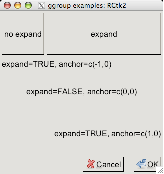
\includegraphics[width=.45\textwidth]{ex-gWidgets-ggroup-RGtk2}\quad
  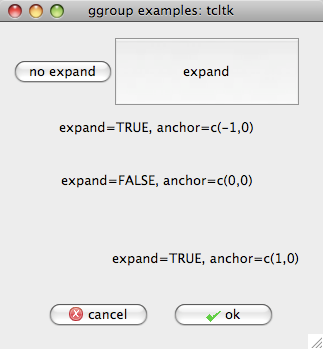
\includegraphics[width=.45\textwidth]{ex-gWidgets-ggroup-tcltk}
 \caption{Use of \code{expand}, \code{anchor}, \code{addSpace} and
     \code{addSpring} with the \code{ggroup} constructor in \pkg{gWidgetsRGtk2} and \pkg{gWidgetstcltk}}
  \label{fig:ggroup-example}
\end{figure}





\begin{Schunk}
\begin{Sinput}
 w  <- gwindow("ggroup examples")
 g  <- ggroup(cont=w, horizontal=FALSE, expand=TRUE)
 g1 <- ggroup(cont=g, expand=TRUE)
 b  <- gbutton("no expand", cont=g1)
 b  <- gbutton("expand", cont=g1, expand=TRUE)
 g2 <- ggroup(cont=g)
 l  <- glabel("expand=TRUE, anchor=c(-1,0)", anchor=c(-1,0), 
             expand=TRUE, cont=g2)
 g3 <- ggroup(cont=g, expand=TRUE)
 l  <- glabel("expand=FALSE, anchor=c(0,0)", anchor=c(0,0), 
             expand=TRUE, cont=g3)
 g4 <- ggroup(cont=g, expand=TRUE)
 l  <- glabel("expand=TRUE, anchor=c(1,0)", anchor=c(1,0), 
             expand=TRUE, cont=g4)
\end{Sinput}
\end{Schunk}
  

This demonstrates how one can use the \meth{addSpace} and \meth{addSpring}
methods to right align buttons in a button bar.
\begin{Schunk}
\begin{Sinput}
 g5 <- ggroup(cont=g, expand=FALSE)
 addSpring(g5)
 cancel  <- gbutton("cancel", cont=g5, handler=function(h,..) {
   dispose(w)
 })
 addSpace(g5, 12)
 ok  <- gbutton("ok", cont=g5)
\end{Sinput}
\end{Schunk}
\end{example}

The next example shows an alternative to the expand group widget.

\begin{example}{The \meth{delete} method of \code{ggroup}}{ex-gWidgets-ggroup-delete}
This example shows nested \code{ggroup} containers and the use of the
\method{delete}{ggroup} method to remove a child widget from a
container. In this application, a box is set aside at the top of the
window to hold a message that can be set via \code{openAlert} and
closed with \code{closeAlert}. This example works better under
\pkg{RGtk2}, as the space allocated to the alert is reclaimed when
it is closed.


This code sets up the area for the alert box to appear from.
\begin{Schunk}
\begin{Sinput}
 w <- gwindow("Alert box example")
 g <- ggroup(horizontal=FALSE, cont = w)
 alertBox <- ggroup(cont = g)
 mainBox <- ggroup(cont = g, expand=TRUE)
 l <- glabel("main box label", cont = mainBox, expand=TRUE)
 ig <- NULL                              # global
\end{Sinput}
\end{Schunk}

These two functions will open and close the alert box respectively. In
this example we use the global value, \code{ig}, to store the inner group.
\begin{Schunk}
\begin{Sinput}
 openAlert <- function(message="message goes here") {
   ig <<- ggroup(cont=alertBox)
   glabel(message, cont = ig)
 }
 closeAlert <- function() {
   if(!is.null(ig))
     delete(alertBox, ig)
   ig <<- NULL
 }
\end{Sinput}
\end{Schunk}

The state of the box can be toggled programmatically via
\begin{Schunk}
\begin{Sinput}
 QT <- openAlert("new message")                # open
 QT <- closeAlert()                            # close
\end{Sinput}
\end{Schunk}

To elaborate on this, one might add a timer to close the alert after a specified
time interval and a close icon so the user may dismiss the alert.
\end{example}


\subsection{The \code{gframe} and \code{gexpandgroup} containers}
\label{sec:gWidgets-decorated-cont}

Framed containers are used to set off elements and are provided by
\constructor{gframe}. Expandable containers are used to preserve
screen space unless requested and are provided by
\constructor{gexpandgroup}. Both of these containers can be used in
place of the \constructor{ggroup} container.

In addition to the \code{ggroup} arguments, the \constructor{gframe}
constructor has the arguments \argument{text}{gframe} to specify the
text marking the frame and \argument{pos}{gframe} to specify the
positioning of the text, using 0 for left and 1 for right. If the
toolkit supports markup, such as \pkg{RGtk2}, the
\argument{markup}{gframe} argument takes a logical indicating if
markup is being used in the specification of \args{text}.  The
\method{names}{gframe} method can be used to get and set the label
after construction of the widget.


The \constructor{gexpandgroup} constructor, like \code{gframe}, has
the \code{text} argument, but no \code{pos} argument for positioning
the text label. The widget has two states, which may be toggled either
by clicking the trigger or through the
\method{visible\ASSIGN}{gexpandgroup} method.  A value of \code{TRUE}
means the child is visible. The
\method{addHandlerChanged}{gexpandgroup} method is used to specify a
callback for when the widget is toggled.

\begin{example}{The \constructor{gframe} and \constructor{gexpandgroup} containers}{gWidgets-gframe-gexpandgroup-ex}
This example shows how the \constructor{gframe} container can be used.
\begin{Schunk}
\begin{Sinput}
 w <- gwindow("gframe example")
 f <- gframe(text="title", pos=1, cont=w)
 l <- glabel("Some text goes here", cont=f)
 names(f) <- "new title"
\end{Sinput}
\end{Schunk}

This is a similar example for \constructor{gexpandgroup}.
\begin{Schunk}
\begin{Sinput}
 w <- gwindow("gexpandgroup example")
 g <- gexpandgroup(text="title", cont=w)
 l <- glabel("Some text goes here", expand=TRUE, cont=g)
 visible(g) <- FALSE
 visible(g) <- TRUE                      # toggle visibility
\end{Sinput}
\end{Schunk}
\end{example}




\section{Paned containers: the \code{gpandedgroup} container}
\label{sec:gWidgets-gpanedgroup-container}

The \constructor{gpanedgroup} constructor produces a container which
has two children which are separated by a visual gutter which can be adjusted using
the mouse to allocate the space between the two children. The children are aligned side-by-side (by default) or
top to bottom if the \argument{horizontal}{gpanedgroup} argument is
given as \code{FALSE}. The sash position can
also be done programatically using the \method{svalue\ASSIGN}{gpanedgroup}
method, where  a value from 0 to 1 specifies the proportion of space allocated to the leftmost (topmost) child.

To add children, the container should be used as the parent container
for two constructors. These can be other container constructors which
is the typical usage for more complicated layouts.
(For toolkits which support the separation of widget
construction and layout, the \constructor{gpanedgroup} constructor can
have two children specified to the arguments
\argument{widget1}{gpanedgroup} and \argument{widget2}{gpanedgroup}.)

\begin{example}{Paned groups}{ex-gWidgets-panedgroups}
  This example shows how one could use this container.
\begin{Schunk}
\begin{Sinput}
 w <- gwindow("gpanedgroup example", visible=FALSE)
 pg <- gpanedgroup(cont=w)
 g <- ggroup(cont=pg)                  # left child
 l <- glabel("left child", cont=g)
 b <- gbutton("right child", cont=pg)
 visible(w) <- TRUE
\end{Sinput}
\end{Schunk}
To adjust the sash position, one can do:
\begin{Schunk}
\begin{Sinput}
 svalue(pg) <- 0.75
\end{Sinput}
\end{Schunk}
\end{example}


  
\section{Tabbed notebooks: the \code{gnotebook} container}
\label{sec:gWidgets-gnotebook}

The \constructor{gnotebook} constructor produces a tabbed notebook
container. The constructor has the argument \argument{tab.pos}{gnotebook}
to specify the location of the tabs. A value of 1 through 4 with 1
being botton, 2 left side, 3 top and 4 right side being used, with the
default being 3. The \argument{closebuttons}{gnotebook} argument takes a logical
indicating whether the tabs should have close buttons on them. In this
case, the argument \argument{dontCloseThese}{gnotebook} can be used to
specify which tabs, by index, should not be closable. (Some toolkits do
not implement these features though.)

The \method{add}{gnotebook} method for the notebook container uses the
\argument{label}{add} argument to specify the tab label. As \meth{add}
is called implicitly when a a widget is constructed, this argument is usually
specified to the constructor.

\paragraph{Methods}
The \method{svalue}{gnotebook} method returns the index of the
currently raised tab, whereas \method{svalue\ASSIGN}{gnotebook} can be
used to switch the page to the specified tab. The currently shown tab can be
removed using the \method{dispose}{gnotebook} method. To remove a
different tab, use this method in combination with
\meth{svalue\ASSIGN}. When removing many tabs, you may want to start
from the end as otherwise the tab positions change, which can be
confusing when using a loop. The \method{names}{gnotebook} method can
be used to retrieve the tab names, and
\method{names\ASSIGN}{gnotebook} to set the names. The
\method{length}{gnotebook} method returns the number of pages held by
the notebook.


\begin{example}{Tabbed notebook example}{ex-gWidgets-gnotebook}
  A simple example follows. The \args{label} argument is passed along from the constructor
  to the \meth{add} method for the notebook instance.
\begin{Schunk}
\begin{Sinput}
 w <- gwindow("gnotebook example")
 nb <- gnotebook(cont=w, tab.pos=3)
 l <- glabel("first page", cont=nb, label="one")
 b <- gbutton("second page", cont=nb, label="two")
\end{Sinput}
\end{Schunk}
To set the page to the first one:
\begin{Schunk}
\begin{Sinput}
 svalue(nb) <- 1
\end{Sinput}
\end{Schunk}
To remove the first page (the current one)
\begin{Schunk}
\begin{Sinput}
 dispose(nb)
\end{Sinput}
\end{Schunk}
\end{example}

\section{Grid layout: the \code{glayout} container}
\label{sec:gWidgets-glayout-container}

The layout of dialogs and forms is usually seen with some form of
alignment between the widgets. The \constructor{glayout} constructor
provides a grid container to do so, using matrix notation to specify location of the children.
The argument
\argument{homogeneous}{glayout} can be used to specify that each cell
take up the same size, the default is \code{FALSE}. Spacing between each cell may be specified through the \argument{spacing}{glayout} argument.

Children may be added to the grid at a specific row and column, and a
child may span more than one row or column. To specify this, \R's
matrix notation, \code{[\ASSIGN}, is used with the indices indicating
the row and column.  When a child is to span more than one row or
column, the corresponding index should be a vector of indices
indicating so.  There is no \code{[} method defined to return the
child components.  
To add a child, the \code{glayout} container should be specfied as the \code{container} and be on the left hand side of the \code{[\ASSIGN} call. For convenience, if the right hand side is a string, a label will be generated.
To align a widget within a cell, the
\argument{anchor}{add} argument of the \code{[\ASSIGN}{glayout} method
is used. The example illustrates how this can be used to achieve a center balance.


\begin{example}{Layout with \constructor{glayout}}{ex-gWidgets-glayout}
  This example shows how a simple form can be given an attractive
  layout using a grid container. It uses the \constructor{gedit}
  constructor to provide a single-line text entry widget. As the
  matrix notation does not have a means to return the child widget (a
  \code{[} method say), we store the values of the
  \constructor{gedit} widgets into variables.
\begin{Schunk}
\begin{Sinput}
 w <- gwindow("glayout example")
 tbl <- glayout(cont=w)
 right <- c(1,0); left <- c(-1,0)
 tbl[1,1, anchor=right] <- "name"
 tbl[1,2, anchor=left ] <- (name <- gedit("", cont=tbl))
 tbl[2,1, anchor=right] <- "rank"
 tbl[2,2, anchor=left ] <- (rank <- gedit("", cont=tbl))
 tbl[3,1, anchor=right] <- "serial number"
 tbl[3,2, anchor=left ] <- (snumber <- gedit("", cont=tbl))
\end{Sinput}
\end{Schunk}
\end{example}







\chapter{\pkg{gWidgets}: Control Widgets}
\section{Basic controls}
\label{sec:gWidgets-controls}
%% orgainze by function

\XXX{Where to integrate methods such as enabled?}
\XXX{stock icons}
\XXX{addHandler text -- done here with first, but could be elsewhere}
\XXX{drag and drop example}
  

  
This section discusses the basic controls provided by
\pkg{gWidgets}.

\begin{table}
\centering
\label{tab:gWidgets-control-widgets}
\caption{Table of constructors for control widgets in \pkg{gWidgets}. Most, but not all, are implemented for each toolkit.}
\begin{tabular}{@{}lp{0.7\textwidth}@{}}
\toprule

Constructor&Description\\
\midrule
\constructor{glabel}&A text label\\\constructor{gbutton}&A button to initiate an action \\\constructor{gcheckbox}&A checkbox\\\constructor{gcheckboxgroup}&A group of checkboxes\\\constructor{gradio}&A radio button group\\\constructor{gcombobox}&A drop-down list of values, possible editable\\\constructor{gtable}&A table (vector or data frame) of values for selection\\\constructor{gslider}&A slider to select from a sequence value\\\constructor{gspinbutton}&A spinbutton to select from a sequence of values\\\constructor{gedit}&Single line of editable text\\\constructor{gtext}&Multi-line text edit area\\\constructor{ghtml}&Display text marked up with HTML\\\constructor{gdf}&Data frame viewer and editor\\\constructor{gtree}&A display for heirarchical data\\\constructor{gimage}&A display for icons and images\\\constructor{ggraphics}&A widget containing a graphics device\\\constructor{gsvg}&A widget to display SVG files\\\constructor{gfilebrowser}&A widget to select a file or directory\\\constructor{gcalendar}&A widget to select a date\\\constructor{gaction}&A resusable definition of an action\\\constructor{gmenubar}&Adds a menubar on a top-level window \\\constructor{gtoolbar}&Adds a toolbar to a top-level window\\\constructor{gstatusbar}&Adds a status bar to a top-level window\\\constructor{gtooltip}&Add a tooltip to widget\\\constructor{gseparator}&A widget to display a horizontal or vertical line
\\ \bottomrule
\end{tabular}
\end{table}%% place these as approporiate
% \begin{table}
%   \centering
%   \begin{tabular}{l@{\quad}p{.75\textwidth}}
% %    \toprule
%     \constructor{glabel} & A text label\\
%     \constructor{gbutton} & A button to initiate an action \\
%     \constructor{gcheckbox} & A checkbox widget\\
%     \constructor{gradio} & Constructs a radio button group\\
%     \constructor{gcheckboxgroup} & Constructs a group of checkboxes\\
%     \constructor{gcombobox} & Constructs drop down list of values\\
%     \constructor{gtable} & Shows a table (vector or data frame) of
%     values for selection\\ 
%     \constructor{gslider} & A slider to select a value\\
%     \constructor{gspinbutton} & A spinbutton to select from a set of values\\
%     \constructor{gedit} & One line of editable text\\
%     \constructor{gtext} & multi-line text edit\\
%     \constructor{ghtml} & Display text marked up with HTML\\
%     \constructor{gdf} & Data frame viewer and editor\\
%     \constructor{gtree} & Displays heirarchical data\\
%     \constructor{gimage} & Displays icons and images\\
%     \constructor{ggraphics} & A widget containing a graphics device\\
%     \constructor{gfilebrowser} & A widget to select a file or directory\\
%     \constructor{gcalendar} & A widget to select a date\\
%     \constructor{gaction} & a resusable definition of an action\\
%     \constructor{gmenubar} & Puts a menubar on a top-level window\\    
%     \constructor{gtoolbar} & Adds a toolbar to a top-level window\\
%     \constructor{gstatusbar} & Adds a status bar to a top-level window\\
%     \constructor{gseparator} & A widget to display a horizontal or vertical line\\
%     \bottomrule
%   \end{tabular}
%   \caption{Table of basic control constructors in \pkg{gWidgets}}
%   \label{tab:gWidgets-control-widgets}  
% \end{table}


\subsection{Buttons, Menubars, Toolbars}
\label{sec:gWidgets-buttons}

The button widget allows a user to initiate an action through clicking on
it. Buttons have labels -- usually verbs indicating action -- and often
icons. The \constructor{gbutton} constructor has an argument
\argument{text}{gbutton} to specify the text.  For text that matches
the stock icons of \pkg{gWidgets}, an icon will also be rendered. A list of stock icons is returned by \code{getStockIcons}. In common with the other controls, the argument
\argument{handler}{gbutton} is used to specify a callback and the
\argument{action}{gbutton} argument will be passed along to this
callback (unless it is a \code{gaction} object, whose case is described
below).

The default handler is the click handler which can be specified at
construction, or afterward through the
\method{addHandlerClicked}{gbutton}.


%% Default
A new button may or may not have the focus when a GUI is
constructed. If it does have the focus, then the \kbd{return} key will
initiate the button click signal. To make a GUI start with its focus
on a button, the \method{defaultWidget}{gWidgets} method is available. 

%% methods
The \method{svalue}{gbutton} method will return a button's label, and
\method{svalue\ASSIGN}{gbutton} is used to set the label text.
Most GUIs will make a button insensitive to user input if the button's
action is not currently permissible. Toolkits draw such buttons in a
greyed out state. The \method{enabled\ASSIGN}{gWidgets} method can set or
disable whether a widget can accept input.

% A basic example of a button with a handler was given in Example~\ref{ex-gWidgets-hello-world-button}.

% As an example of the limitations of \pkg{gWidgets} compared to the
% underlying toolkits, within \pkg{gWidgets} there are no methods to set
% an icon, or add an mnemonic to the button.


% \begin{example}{Hello world button}{ex-gWidgets-hello-world-button}
%   This example shows how a button is assigned a handler to respond to
%   click events.~\footnote{Each toolkit has its idiosyncracies. If this
%     example is run using \pkg{RGtk2} the button will stretch to fill
%     the space. At times this is not desired. Placing the button within
%     a \code{ggroup} container can prevent this. Whereas, under
%     \code{tcltk} the parent window will shrink to fit the button. The
%     \meth{size} method can prevent this if it is not desired.} When
%   working with handlers, one can use an object name that will be found
%   through \R's scoping rules, or the components passed through the
%   \code{h} argument, as below.

% <<>>=
% w <- gwindow("Button example")
% b <- gbutton("Click me", cont=w)
% id <- addHandlerChanged(b, action=w, handler=function(h,...) {
%   btnText <- svalue(h$obj)                   # or svalue(b)
%   svalue(h$obj) <- paste("don't", btnText, "again") # set text
%   enabled(h$obj) <- FALSE
%   svalue(h$action) <- "Button example is finished" # set title
% })

% @ 

% \end{example}





\subsection{Actions}
\label{sec:gWidgets-actions}

In GUI programming an action is a reusable code object that can be
shared among buttons, toolbars, and menubars. Common to these three
controls are that the user expects some ``action'' to occur when a
value is selected. For example, some save dialog is summoned, or some
page is printed.
%%In the command framework, actions initiate commands.
Actions contain enough information to be displayed in several
manners. An action would contain some text, an icon, perhaps some
keyboard accelerator, and some handler to call when the action is
selected. When a particular action is not possible due to the state of
the GUI, it should be disabled, so as not to be sensitive to user interaction.

Actions in \pkg{gWidgets} are created through the
\constructor{gaction} contstructor. The arguments are
\argument{label}{gaction}, \argument{tooltip}{gaction},
\argument{icon}{gaction}, \argument{key.accel}{gaction} and the
standard \argument{handler}{gaction} and
\argument{action}{gaction}. The label appears as the text on a button,
the menu item or toolbar text, whereas the icon will decorate the same
if possible. For some toolkits, the tooltip pops up when the mouse hovers.
(See also the \meth{tooltip\ASSIGN} method.)

\paragraph{methods}
The main methods for actions are \method{svalue\ASSIGN}{gaction} to
set the label text and \method{enabled\ASSIGN}{gaction} to adjust
whether the widget is sensitive to user input. All instances of the
action are set through one call. In some toolkits, such as
\pkg{RGtk2}, actions are bundled together into action groups. This
grouping allows one to set the sensitivity of related actions at
once. In \R, one can store like actions in a list, and get similar
functionality by using \code{sapply}, say.

\paragraph{buttons}
An action can be assigned to a button by setting it as the
\argument{action}{gbutton} argument of the \code{gbutton} constructor, in which
case all other arguments for the constructor are ignored. 

Otherwise, actions are used as list components which define the
toolbar or menubar, as described in the following.



\subsection{Toolbars}
\label{sec:gWidgets-toolbars}
Toolbars and menubars are implemented in \pkg{gWidgets} using
\code{gaction} items. Toolbars (and menubars) are specified using a named
list of menu components. This is similar to how \pkg{RGtk2} can use an XML specification
to define a user interface, but unlike how menubars and toolbars can
be created one item at a time in the toolkits.

For a toolbar, the list has a simple structure. The list has named
components each of which either describes a toolbar item or a
separator. The toolbar items are specified by \code{gaction} instances
and separators by \code{gseparator} instances with no container
specified.


The \constructor{gtoolbar} constructor takes as its first argument the
list.  As toolbars belong to the window, the corresponding
\pkg{gWigdets} objects use a \constructor{gwindow} object as the
parent container. (Some of the toolkits relax this.)  The argument
\argument{style}{gtoolbar} can be one of \qcode{both},
\qcode{icons}, \qcode{text}, or \qcode{both-horiz} to specify how
the toolbar is rendered. Toolbars in \pkg{gWidgetstcltk} are not
native widgets, so the implementation uses aligned buttons.




\subsection{Menubars, popup menus}
\label{sec:gWidgets-menubars}

Menubars and popup menus are specified in a similar manner as toolbars with menu items
being defined through \code{gaction} instances, and visual separators
by \code{gseparator} instances. Menus differ from toolbars, as
sub-menus give a nested structure. This structure is specified using a
nested list as the component to describe the sub menu. The lists all
have named components, in this case the corresponding name is used to
label the sub menu item. For menu bars, it is typical that all the
top-level components be lists, but for popup menus, this wouldn't
necessarily be the case.

In Mac OS X with a native toolkit, menubars may be drawn along the top
of the screen, as is the custom of that OS. 

\paragraph{Methods}
The main methods for toolbar and menubar instances are
the \method{svalue}{gmenu} method which will return the list. Whereas, the
\method{svalue\ASSIGN}{gmenu} method can be used to redefine the
menubar or toolbar. Use the \method{add}{gmenu} method to append to an
existing menubar or toolbar, again using a list to specify the new items.


\begin{example}{Menubar and toolbar example}{ex-gWidgets-menu-tool-status-bars}

The following commands create some standard looking actions. The
handler \code{f} is just a stub to be replaced in a real application.
\begin{Schunk}
\begin{Sinput}
 f <- function(...) print("stub")        # a stub
 aOpen <- gaction("open", icon="open", handler = f)
 aQuit <- gaction("quit", icon="quit", handler = f)
 aUndo <- gaction("undo", icon="undo", handler = f)
\end{Sinput}
\end{Schunk}

A menubar and toolbar are specified through a list with named components, as is
illustrated next. The menubar list uses a nested list with
named components to specify a submenu.
\begin{Schunk}
\begin{Sinput}
 tl <- list(open = aOpen, quit = aQuit)
 ml <- list(File = list(
              open = aOpen, 
              sep = gseparator(), 
              quit = aQuit),
            Edit = list(
              undo = aUndo
              ))
\end{Sinput}
\end{Schunk}


Menubars and toolbars are added to top-level windows, so their parent
containers are \code{gwindow} objects.
\begin{Schunk}
\begin{Sinput}
 w <- gwindow("Example of menubars, toolbars")
 mb <- gmenu(ml, cont=w)
 tb <- gtoolbar(tl, cont=w)
 l <- glabel("Test of DOM widgets", cont=w)
\end{Sinput}
\end{Schunk}


By disabling a \code{gaction} instance, we change the sensitivity of
all its realizations. Here this will only affect the menu bar.

\begin{Schunk}
\begin{Sinput}
 enabled(aUndo) <- FALSE
\end{Sinput}
\end{Schunk}

An ``undo'' menubar item, often changes its label when a new command
is performed, or the previous command is undone. The
\method{svalue\ASSIGN}{gaction} method can set the label text. This
shows how a new command can be added and how the menu item can be made
sensitive to mouse events.
\begin{Schunk}
\begin{Sinput}
 svalue(aUndo) <- "undo: command"
 enabled(aUndo) <- TRUE
\end{Sinput}
\end{Schunk}

%%\XXX{Citation needed}

Good GUI building principles suggest that one should not replace
values in the a menu, rather one should simply disable those that are
not being used. This allows the user to more easily become familiar
with the possible menu items. However, it may be useful to add to a
menu or toolbar. The \method{add}{gmenu} method can do so. For
example, to add a help menu item to our example one could do:
\begin{Schunk}
\begin{Sinput}
 hl <- list(help = list(
              help = gaction("manual", handler=f)
              ))
 add(mb, hl)
\end{Sinput}
\end{Schunk}




        
\end{example}

\paragraph{Popup menus}

Popup menus can be created for a right click event through the
\constructor{add3rdMousePopupmenu} constructor. (Or
\kbd{control-button-1} for Mac OS X.) This constructor has arguments
\code{obj} to specify a widget, like a button, to initiate the popup,
\argument{menulist}{gmenu} to specify the menu and optionally an
\argument{action}{gmenu} argument.


\begin{example}{Popup menus}{ex-gWidgets-context-menus}
\begin{Schunk}
\begin{Sinput}
 w <- gwindow("Popup example")
 b <- gbutton("click me or right click me", cont=w, 
              handler=function(h, ...) {
                cat("You clicked me\n")
              })
 f <- function(h,...) cat("you right clicked on", h$action)
 mbList <- list(one = gaction("one", action="one", handler=f),
                two = gaction("two", action="two", handler=f)
                )
 add3rdMousePopupmenu(b, mbList)
\end{Sinput}
\end{Schunk}

\end{example}


\section{Text widgets}
\label{sec:text-widgets}

A number of widgets are geared toward the display or entry of
text. The \pkg{gWidgets} API defines \constructor{glabel} for
displaying a single-or multiple-line string of static text,
\constructor{gstatusbar} to place message labels at the foot of a
window, \constructor{gedit} for a single line of editable text, and
\constructor{gtext} for multi-line, editable text. For some toolkits,
a \constructor{ghtml} widget is also defined, but neither \code{RGtk2}
or \code{tcltk} have this implemented.

\subsection{Labels}
\label{sec:gWidgets-static-text}

The \constructor{glabel} constructor produces a basic label
widget. The label's text is specified through the
\argument{text}{glabel} argument. This is a character vector of length
1 or is coerced into one by collapsing the vector with newlines. The
\method{svalue}{glabel} method will return the text as a single
string, and the \method{svalue\ASSIGN}{glabel} method can be used to
set the text programatically. The \method{font\ASSIGN}{glabel} method
can also be used to set the text markup
(Table~\ref{tab:gWidgets-font-properties}).  For some toolkits, the
argument \argument{markup}{glabel} for the constructor takes a logical
value indicating if the text is in the native markup language (PANGO
for \code{RGtk2}).


The widget constructor also has the argument
\argument{editable}{glabel}, which when specified as \code{TRUE} will
add a handler to the event that the label is clicked that allows the
text to be edited.  Although this is popular in some familiar
interfaces, say the tab in a spreadsheet, it has not proven to be
intuitive to most users, as typically labels are not expected to
change.


\subsection{Statusbars}
\label{sec:gWidgets-statusbars}

Statusbars are simply labels placed at the bottom of a window to leave
informative, but non-disruptive, messages for the user.  The
\constructor{gstatusbar} constructor provides this widget.  The argument
\argument{text}{gstatusbar} can be given to set the intial text away
from its default of no message. Subsequent changes are made through
the \method{svalue\ASSIGN}{gstatusbar} method. As with toolbars and
menubars, a top-level window should be specified for the
\argument{container}{gstatusbar} argument.



\subsection{Single-line, editable text}
\label{sec:gWidgets-single-line-editable}

The \constructor{gedit} constructor produces a widget to display a
single line of editable text. The initial text can be set through the
\argument{text}{gedit} argument. 
If it is desirable to set the width of the widget, the
\argument{width}{gedit} argument allows the specification in terms of
number of characters allowed to display without horizontal scrolling. The width
of the widget may also be specified in pixel size through the
\method{size}{gWidgets} method.


\paragraph{Methods}
The text is returned by the
\method{svalue}{gedit} method and may be set through the
\method{svalue\ASSIGN}{gedit} method.
The \meth{svalue} method will return a character vector by
default. However, it may be desirable to use this widget to collect
numeric values or perhaps some other type of variable. One could write
code to coerce the character to the desired type, but it is sometimes
convenient to have the return value be a certain non-character
type. In this case, the \argument{coerce.with}{gedit} argument can be
used to specify a function of a single argument to call before the
value is returned by \meth{svalue}.

Some toolkits allow type-ahead values to be set. These values
anticipate what a user wishes to type and offers a means to complete a
word. The \method{[\ASSIGN}{gedit} method allows these values to be
specifed through a character vector, as in \code{obj[] \ASSIGN\/ values}.



\paragraph{Handlers}
The default handler for the \constructor{gedit} widget is called when
the text area is ``activated'' through the
\kbd{return} key being pressed. Use \meth{addHandlerBlur} to add a
callback for the event of losing focus. The
\method{addHandlerKeystroke}{gedit} method can assign a handler to be
called when a key is released. For the toolkits that support it, the
specific key is given in the \code{key} component of the list \code{h} (the first component).

\begin{example}{Validation}{ex-gWidgets-gedit-validation}
In web programming it is common to have textarea entries be validated
prior to their values being submitted. By validating ahead of time,
the programmer can avoid the lag created by communicating with the
server when the input is not acceptable. However, despite
this lag not being the case for the GUIs considered now, it may still be a
useful practice to validate the values of a text area when the
underlying handlers are expecting a specific type of value.
  
The \args{coerce.with} argument can be used to specify a function
to coerce values after an action is initiatied, but in this example we
show how to validate the text widget when it loses focus. If the value
is invalid, we set the text color to red.


\begin{Schunk}
\begin{Sinput}
 w <- gwindow("Validation example")
 validRegexpr <- "[[:digit:]]{3}-[[:digit:]]{4}"
 tbl <- glayout(cont=w)
 tbl[1,1] <- "Phone number (XXX-XXXX)"
 tbl[1,2] <- (e <- gedit("", cont = tbl))
 tbl[2,2] <- (b <- gbutton("submit", cont = tbl, 
                           handler=function(h,...) print("hi")))
 ## Blur is focus out event
 addHandlerBlur(e, handler = function(h,...) {
   curVal <- svalue(h$obj)
   if(grepl(validRegexpr, curVal)) {
     font(h$obj) <- c(color="black")
   } else {
     font(h$obj) <- c(color="red")
     focus(h$obj) <- TRUE
   }
 })
\end{Sinput}
\end{Schunk}
\end{example}

\subsection{Multi-line, editable text}
\label{sec:gWidgets-multi-line-editable}

The \constructor{gtext} constructor produces a multi-line text editing
widget with scrollbars to accommodate large amounts of text. The
\argument{text}{gtext} argument is for specifying the intial
text. The initial width and height can be
set through similarly named arguments, which is useful under
\pkg{tcltk}. 

The \method{svalue}{gtext} method retrieves the text stored in the
buffer. If the argument \code{drop=TRUE} is specified, then only the
currently selected text will be returned. Text in multiple lines is
returned as a single string with ``\backslashn'' separating the lines.

The contents of the text buffer can be replaced with the
\method{svalue\ASSIGN}{gtext} method. To clear the buffer, the
\method{dispose}{gtext} method can be used.To add text to a buffer, the
\method{insert}{gtext} method is used. The signature is
\code{insert(obj,text)} where \code{text} is a character vector. New text
is added to the end of the buffer, by default, but the
\argument{where}{insert} argument can specify \qcode{beginning} or \qcode{at.cursor}.

As with, \code{gedit}, the \method{addHandlerKeystroke}{gtext} method is used
to set a handler to be called for each keystroke. This is the default handler.

Fonts can be specified for the entire buffer or the selection using
the specifications in Table~\ref{tab:gWidgets-font-properties}. To
specify fonts for the entire buffer use the
\argument{font.attr}{gtable} argument of the constructor. As well, the
\method{font\ASSIGN}{gtext} method can be used, provided there is no
selection when called. If there is a selection, only that text will get the specified
font attributes. Finally, the \argument{font.attr}{insert} argument
for the \meth{insert} method can also be specified to give font
attributes to the newly added text.

\begin{table}
\centering
\label{tab:gWidgets-font-properties}
\caption{Possible specfications for setting font properties. Font values of an object are changed with named vectors, as in \code{font(obj)\ASSIGN c(weight="bold", size=12, color="red")}}
\begin{tabular}{@{}lp{0.6\textwidth}@{}}
\toprule

Attribute&Possible value\\
\midrule
weight&light, normal, bold\\style&normal, oblique, italic\\family&normal, sans, serif, monospace\\size&a point size, such as 12\\color&a named color
\\ \bottomrule
\end{tabular}
\end{table}
\begin{example}{A calculator}{ex-gWidgets-calculator}
%% A calculator layout example
The following example shows how one might use the widgets just
discussed to make a GUI that resembles a calculator. Such a GUI may offer
familiarity to new \R\/ users, although certainly is no replacement
for a command line.

The \constructor{glayout} container is used to neatly arrange the
widgets. This example illustrates how a child widget can span a block
of multiple cells by using the appropriate indexing. Furthermore, the
\args{spacing} argument is used to tighten up the appearance. The
example also illustrates a useful strategy of storing the widgets
using a list for subsequent manipulations.

The following sets up the layout of the display and buttons.
\begin{Schunk}
\begin{Sinput}
 buttons <- rbind(c(7:9, "(", ")"),
                  c(4:6, "*", "/"),
                  c(1:3, "+", "-"))
 bList <- list()
 w <- gwindow("glayout for a calculator")
 g <- ggroup(cont=w, expand=TRUE, horizontal=FALSE)
 tbl <- glayout(cont=g, spacing=2)
 tbl[1, 1:5, anchor=c(-1,0)] <-          # span 5 columns
   (eqnArea <- gedit("", cont=tbl))
 tbl[2, 1:5, anchor=c(1,0)] <- 
   (outputArea <- glabel("", cont=tbl))
 for(i in 3:5) {
   for(j in 1:5) {
     val <- buttons[i-2, j]
     tbl[i,j] <- (bList[[val]] <- gbutton(val, cont=tbl))
   }
 }
 tbl[6,2] <- (bList[["0"]] <- gbutton("0", cont=tbl))
 tbl[6,3] <- (bList[["."]] <- gbutton(".", cont=tbl))
 tbl[6,4:5] <- (eqButton <- gbutton("=", cont=tbl))
 outputArea <- gtext("", cont = g)
\end{Sinput}
\end{Schunk}

This code defines the handler for each button except the equals button
and then assigns the handler to each button. This is done efficiently,
using the generic \meth{addHandlerChanged}. The handler simply pastes
the text for each button into the equation area.

\begin{Schunk}
\begin{Sinput}
 addButton <- function(h, ...) {
   curExpr <- svalue(eqnArea)
   newChar <- svalue(h$obj)              # the button's value
   svalue(eqnArea) <- paste(curExpr, newChar, sep="")
   svalue(outputLabel) <- ""             # clear label 
 }
 out <- sapply(bList, function(i) 
               addHandlerChanged(i, handler=addButton))
\end{Sinput}
\end{Schunk}

When the equals sign is clicked, the expression is evaluated and if
there are no errors, the output is displayed in the label.
\begin{Schunk}
\begin{Sinput}
 addHandlerClicked(eqButton, handler = function(h,...) {
   curExpr <- svalue(eqnArea)
   out <- try(capture.output(eval(parse(text=curExpr))), silent=TRUE)
   if(inherits(out,"try-error")) {
     galert("There is an error")
   } else {
     svalue(outputArea) <- out
     svalue(eqnArea) <- ""            # restart
   }
 })
\end{Sinput}
\end{Schunk}

\end{example}

\section{Selection controls}
\label{sec:gWidgets-widg-select-data}

A common task for a GUI control is to select a value or values from a
set of numbers or a table of numbers. Many toolkits implement these
widgets using a model-view-controller paradigm whereby the control is
just one of possibly many views of the data store (the model). This
approach isn't taken with \pkg{gWidgets}. Rather, each widget has its
own data store (like a vector or data frame)
containing the data for selection, and familar \R\/ methods are used to
manipulate this underlying data store. The controls in \pkg{gWidgets} that
display such data have the methods \code{[}, \code{[\ASSIGN},
\code{length}, \code{dim}, \code{names} and \code{names\ASSIGN}, as
appropriate.

This section discusses several different controls that do basically the
same thing, but which exist primarily because they use screen space differently.


\subsection{Checkbox widget}
\label{sec:gWidgets-checkbox-widget}

The simplest selection control is the \constructor{checkbox} widget
that allows the user to set a state as \code{TRUE} or
\code{FALSE}. The constructor has an argument
\argument{text}{gcheckbox} to set a label and
\argument{checked}{gcheckbox} to indicate if the widget should
initially be checked. The default is \code{TRUE}.

The \method{svalue}{gcheckbox} method returns a logical indicating if
the widget is in the checked state. Use \method{svalue\ASSIGN}{gcheckbox} to set
the state. The label's value is returned by the
\method{[}{gcheckbox} method, and can be adjusted through 
\method{[\ASSIGN}{gcheckbox}.

The default handler would be called on a click event, when the state toggles. If it is desired
that the handler be called only in the \code{TRUE} state, say, one
needs to check within the handler for this.

\subsection{Radio button widget}
\label{sec:gWidgets-radio-button-widget}

A radio button group allows the user to choose one of a few
items. A radio button group object is returned by
\constructor{gradio}. The items to choose from are specified as a
vector of values to the \argument{items}{gradio} argument. These items
may be displayed horizontally or vertically (the default) as specified by the
\argument{horizontal}{gradio} argument which expects a logical. The
\argument{selected}{gradio} argument specifies the initially selected item,
with a default of the first.

The currently selected item is returned by \method{svalue}{gradio} as
the label text or by the index if the argument \args{index} is
\code{TRUE}. The item may be set with the
\method{svalue\ASSIGN}{gradio} method. Again, the item may be
specified by the label or by an index, the latter when the argument
\code{index=TRUE} is specified. The data store is the set of labels so
are referenced through the \method{[}{gradio} method, and may be set
(if the underlying toolkit allows it) with the
\method{[\ASSIGN}{gradio} method. (In \pkg{gWidgetstcltk} one can not
change the number of radio buttons.) For convenience, the
\method{length}{gradio} method returns the number of labels.

The default handler would be called on a click event.

\subsection{A group of checkboxes}
\label{sec:gWidgets-group-checkboxes}


The checkbox group widget, produced by the
\constructor{gcheckboxgroup} constructor, is similar to a radio group,
but allows the selection of one or more of a set of items.  The
\argument{items}{gcheckboxgroup} arugment is used to specify the
values. The state of whether an item is selected can be set with a
logical vector of the same size as the number of items to the
\argument{checked}{gcheckboxgroup} argument, recycling is used. The
item layout can be controlled by the
\argument{horizontal}{gcheckboxgroup} argument. The default is a
vertical layout (\code{horizontal=FALSE}).

The state is retrieved as a character vector through the
\method{svalue}{gcheckboxgroup} method. The \code{index=TRUE} argument
instructs \meth{svalue} to return the indices instead. As a
checkboxgroup is like both a checkbox and a radio button group, one
can set the selected values two different ways. As with a checkbox, 
the selected values can be set by specifying a logical vector through the
\method{svalue\ASSIGN}{gcheckboxgroup} method. As with radio button groups,
the selected values can also be set with a character vector indicating
which labels should be selected, or if \code{index=TRUE} is given,
using a numeric index vector.

The labels are returned through the \method{[}{gcheckboxgroup} method
and if the underlying toolkit allows it, set through the
\method{[\ASSIGN}{gcheckboxgroup} method. As with \constructor{gradio},
the \method{length}{gcheckboxgroup} method returns the number of items.

\subsection{A combobox}
\label{sec:gWidgets-combobox}

A combobox is used as an alternative to a radio button group when
there are too many choices to comfortably fit on the screen. Comboboxes are
constructed by \constructor{gcombobox}. The possible choices are specified to the argument
\argument{items}{gcombobox}. This may be a vector of values or a data
frame whose first column defines the choices. For toolkits which
support icons in the combobox, if the data is specified as a data
frame, the second column can be used to signify which stock icon is to
be used. By design, a third column can be used to specify a tooltip,
but this is not implemented for \pkg{RGtk2} and \pkg{tcltk}. 

The argument \argument{editable}{gcombobox} accepts a logical value
indicating if the user can supply their own value by typing into a
text entry area. The default is \code{FALSE}. When editing is possible, the constructor also
has the \argument{coerce.with}{gcombobox} argument like
\code{gedit}.

The currently selected value is returned through the
\method{svalue}{gcombobox} method. If \args{index} is \code{TRUE}, the
index of the selected item is given if possible. The state can be set
through the \method{svalue\ASSIGN}{gcombobox} method. This is
specified by a character unless \args{index} is \code{TRUE}, in which
case as a numeric index with respect to the underlying items. The
\method{[}{gcombobox} method returns the items of the data store, and
\method{[\ASSIGN}{gcombobox} is used to assign new values to the data
store. The value may be a vector, or data frame if an icon or tooltip
is being assigned. The \method{length}{gcombobox} method returns the
number of items.

The default handler is called when the state of the widget is
changed. This is also aliased to
\method{addHandlerClicked}{gcombobox}. When \code{editable} is
\code{TRUE}, then the \method{addHandlerKeystroke}{gcombobox} can be
used to set a handler to response to keystroke events.


\begin{example}{Selection widgets}{ex-gWidgets-selection-widgets}
\begin{figure}
  \centering
  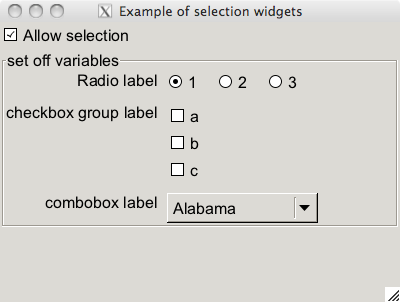
\includegraphics[width=.65\textwidth]{ex-gWidgets-selection-widgets}
  \caption{A template for a GUI using some of the widgets for selection.}
  \label{fig:ex-gWidgets-selection-widgets}
\end{figure}

This example provides template for a possible GUI that would allow a
specification of arguments for a function
(Figure~\ref{fig:ex-gWidgets-selection-widgets}).  A checkbox is
used to toggle whether the other controls are enabled or not.
\begin{Schunk}
\begin{Sinput}
 w <- gwindow("Example of selection widgets", visible=FALSE)
 g <- ggroup(horizontal=FALSE, cont=w)
 cb <- gcheckbox("Allow selection", cont=g, checked=FALSE, 
                 handler = function(h, ...) {
                   enabled(f) <- svalue(cb)
                 })
 f <- gframe("set off variables", cont=g)
 tbl <- glayout(cont=f)
 right <- c(1, 1); left <- c(-1, 1)
 tbl[1,1, anchor=right] <- "Radio label"
 tbl[1,2, anchor=left]  <- (rb <- gradio(1:3, horizontal=TRUE, 
            cont = tbl))
 tbl[2,1, anchor=right] <- "checkbox group label"
 tbl[2,2, achor=left] <- (chb <- gcheckboxgroup(letters[1:3], 
            horizontal=FALSE, cont = tbl))
 tbl[3,1, anchor=right] <- "combobox label"
 tbl[3,2, achor=left] <- (combo <- gcombobox(state.name, 
            cont = tbl))
 enabled(f) <- svalue(cb)                # match
 visible(w) <- TRUE
\end{Sinput}
\end{Schunk}
               
    
\end{example}

\subsection{Display of tabular data}
\label{sec:gWidgets-tabular-data-display}


The \constructor{gtable} constructor produces a widget that displays
data in a tabular form from which the user can select one (or more)
rows. The widgets performance under \pkg{gWidgetsRGtk2} is much faster
and able to handle larger data stores than under \pkg{gWidgetstcltk},
as there is no native table widget in \tcltk, and under
\pkg{gWidgetsQt}. All perform well on moderate-sized data sets (10 or
so columns and fewer than 500 rows),

The data is specified through the \argument{items}{gtable}
argument. This may be a data frame, matrix or vector. Vectors and
matrices are coerced to data frames, with characters as strings not
factors.  The data is presented in a
tabular form, with column headers derived from the \code{names}
attribute of the data frame.  

The \argument{icon.FUN}{gtable} argument
is used to place a stock icon in a left-most column.  This argument
takes a function of a single argument -- the data frame being shown --
and should return a character vector of stock icon names, one for each
row.

\paragraph{Selection}
Users can select a row, not a cell from this widget. The value returned by a selection is
controlled by the constructor's arguments \argument{chosencol}{gtable}, which
specifies which column value will be returned, as the user can only
specify the row; and \argument{multiple}{gtable} which controls
whether the user may select more than one row.  


\paragraph{Methods}
The \method{svalue}{gtable} method will return the currently selected
value. If the argument \code{index} is specified as \code{TRUE}, then
the selected row index (or indices) will be returned. These refer to
the data store, not the visible data when filtering is being used (below). The
argument \code{drop} specifies if just the chosen column's value is
returned (the default) or, if specified as \code{FALSE}, the entire row.
 
The underlying data store is referenced by the \method{[}{gtable}
method. Indices may be used to access just a portion. Values may be
set using the \method{[\ASSIGN}{gtable} method, but be warned it is
not as flexible as assigning to a data frame. The underlying
toolkits may not like to change the type of data displayed in a
column, so when updating a column do not assume some underlying
coercion, as is done with \R's data frames. To replace the data store, the \code{[\ASSIGN} can
be used via \code{obj[] \ASSIGN\/ new\_data\_frame}. The methods
\method{names}{gtable} and \method{names\ASSIGN}{gtable} refer to the
column headers, and \method{dim}{gtable} and \method{length}{gtable}
the underlying dimensions of the data store.

\paragraph{Handlers}
Selection is done through a single click. The \method{addHandlerClick}{gtable}
method can be used to assign a handler to those events. The default
handler, \method{addHandlerDoubleclick}{gtable}, will assign a
handler for a double click event. Also of interest are the
\method{addHandlerRightclick}{gtable} and
\method{add3rdMousePopupMenu}{gtable} methods for assigning handlers
to  right-click events.

\paragraph{Filtering}
The arguments \argument{filter.column}{gtable} and
\argument{filter.FUN}{gtable} allow one to specify whether the user
can filter, or limit, the display of the values in the data store. If
a column number is specified to \code{filter.column} then a combobox
is added to the widget with values taken from the unique values in the
specified column. Changing the value of the combobox, restricts the
display of the data to just those rows which match that column's
values. More advanced filtering can be specified using the
\argument{filter.FUN}{gtable} argument. If this is a function, then it takes
arguments \code{(data\_frame, filter.by)} where the data frame is the
data, and the \code{filter.by} value is the state of a combobox whose
values are specified through the argument
\argument{filter.labels}{gtable}. This function should return a logical
vector with length matching the number of rows in the data frame.
Only rows corresponding to \code{TRUE} values will be displayed. If
\code{filter.FUN} is the character string ``\code{manual}'' then the
\method{visible\ASSIGN}{gtable} method can be used to control the
filtering, again by specifying a logical vector of the proper
length. See Example~\ref{ex-gWidgets-filter-gtable} for an
application.


The \constructor{gtable} widget shows clearly the trade offs between
using \pkg{gWidgets} and a native toolkit under \R. As will be seen in
later chapters, setting up a table to display a data frame using the
toolkit packages directly can involve a fair amount of
coding as compared to \constructor{gtable}, which makes it very
easy. However, there is far less power possible from
\pkg{gWidgets}. For example, there is no method to adjust the column
sizes programatically (although they can be adjusted with the
mouse),there is no means to adjust the formatting of the displayed
text, or to embed other widgets into the tabular display.

\begin{example}{Simple filtering}{ex-gWidgets-simple-filter-gtable}
  We use the \code{Cars93} data set from the \pkg{MASS} package to
  show how to set up a display of the data which provides simple
  filtering based on the type of car, whose value is stored in column 3.
  
\begin{Schunk}
\begin{Sinput}
 require(MASS)
 w <- gwindow("gtable example")
 tbl <- gtable(Cars93, chosencol=1, filter.column=3, cont=w)
\end{Sinput}
\end{Schunk}

Adding a handler for the double click event is illustrated bleow. This
handler prints both the manufacturer and the model of the currently
selected row when called.
\begin{Schunk}
\begin{Sinput}
 addHandlerChanged(tbl, handler=function(h,...) {
   val <- svalue(h$obj, drop=FALSE)
   cat(sprintf("You selected the %s %s", val[,1], val[,2]))
 })
\end{Sinput}
\end{Schunk}
%%$ emacs
\end{example}


\begin{example}{More complex filtering}{ex-gWidgets-filter-gtable}
%% Example of hand-built filter using gtable

Even with moderate-sized data sets, the number of rows can be quite large, in which case it is
inconvenient to use a GUI for selection unless some means of searching or filtering the
data is used. This example uses the possible CRAN sites, to show how a
\code{gedit} instance can be used as a search box to filter the display of
data. The \code{addHandlerKeystroke} method is used so that the search
results are updated as the user types.


The \code{available.packages} function returns a data frame of all
available packages. If a CRAN site is not set, the user will be
queried to set one.
\begin{Schunk}
\begin{Sinput}
 d <- available.packages()       # pick a cran site
\end{Sinput}
\end{Schunk}

This basic GUI is barebones, for example we skip adding text labels to guide the user. 
\begin{Schunk}
\begin{Sinput}
 w <- gwindow("test of filter")
 g <- ggroup(cont=w, horizontal=FALSE)
 ed <- gedit("", cont=g)
 tbl <- gtable(d, cont=g, filter.FUN="manual", expand=TRUE)
\end{Sinput}
\end{Schunk}
The \argument{filter.FUN}{gtable} provides a means to have a combobox
control the display of the table. For this example, we desire more
flexibility, so we specify the value of \qcode{manual}.

Different search criteria may be desired, so it makes sense to
separate out this code from the GUI code using a function. The one below
uses \code{grep} to match, so that regular expressions can be
used. Another reasonable choice would be to use the first letter of
the package. (That filtering could also be specified easily through the
\argument{filter.FUN}{gtable} argument.)

\begin{Schunk}
\begin{Sinput}
 ourMatch <- function(curVal, vals) {
   ind <- grep(curVal, vals)             # indices
   vis <- rep(FALSE, length(vals))
   if(length(ind) > 0)
     vis[ind] <- TRUE
   return(vis)                           # logical
 }
\end{Sinput}
\end{Schunk}

Finally, the \code{addHandlerKeystroke} method calls its handler
everytime a key is released while the focus is in the edit widget. In
this case, the handler finds the matching indices using the
\code{ourMatch} function, converts these into logical format, and then
updates the display using the \meth{visible\ASSIGN} method for
  \code{gtable}.
\begin{Schunk}
\begin{Sinput}
 id <- addHandlerKeystroke(ed, handler=function(h, ...) {
   vals <- tbl[, 1, drop=TRUE]
   curVal <- svalue(h$obj)
   vis <- ourMatch(curVal, as.character(vals))
   visible(tbl) <- vis
 })
\end{Sinput}
\end{Schunk}
\end{example}



\subsection{An editor for tabular data}
\label{sec:gWidgets-an-editor-tabular}

The \constructor{gdf} constructor returns a widget for editing data
frames. This is similar to the GUI provided by the \code{data.entry}
function, but uses the underlying toolkit in use by
\pkg{gWidgets}. Each cell can be edited. Users can click (or double
click) in a cell to select it, or use the arrow and \kbd{tab} keys to
navigate. For \pkg{gWidgetstcltk}, there is no native widget for
editing tabular data, so the \code{tktable}, add-on widget is used
(\url{tktable.sourceforge.net}). A warning will be issued if this is
not installed. Again, the widget under \pkg{gWidgetsRGtk2} is much
faster than that under \pkg{gWidgetstcltk}, but both can load a
moderately sized data frame in a reasonable time. (For
\pkg{gWidgetsRGtk2} there is also the \constructor{gdfedit}
constructor, which is faster and has better usability features.)

The constructor has argument \argument{items}{gdf} to specify the data
frame to edit and \argument{name}{gdf} to specify the data frame name,
if desired. The column types are important, in particular factors and
character types are treated differently, although they may render in a
similar manner.

\paragraph{Methods} There are several methods defined that follow
those of a data frame. The \method{[}{gdf} and \method{[\ASSIGN}{gdf}
methods can be used to extract and set values from the data frame by
index. As with \code{gtable}, these are not as flexible as for a data
frame though. In particular, it may not be possible to changes the
type of a column, or add new rows or columns through these
methods. Using no indices, as in \code{obj[,]} will return the current
data frame, which can be assigned to some value for saving. The
current data frame can be completely replaced, when no indices are
specified in the replacement call. Additionally, the data frame
methods \method{dimnames}{gdf}, \method{dimnames\ASSIGN}{gdf},
\method{names}{gdf}, \method{names\ASSIGN}{gdf}, and
\method{length}{gdf} are defined.

The following can be used to assign handlers:
\method{addHandlerChanged}{gdf} (cell changed),
\method{addHandlerClicked}{gdf}, \method{addHandlerDoubleclick}{gdf},
\method{addHandlerColumnClicked}{gdf},
\method{addHandlerColumnDoubleclick}{gdf}, and
\method{addHandlerColumnRightclick}{gdf}.


The \constructor{gdfnotebook} constructor produces a notebook that can hold several data frames at once.

\section{Selection from a sequence of numbers}
\label{sec:gWidgets-select-from-sequ}

The previous widgets allowed selection from a user-specified set of
values. When these values are a sequence of numbers, the slider
control and spin button control are also commonly used. Both of these
widgets have arguments to specify the sequence that match those of the
\code{seq} function in \R: \argument{from}{gslider},
\argument{to}{gslider}, and \argument{by}{gslider}.

\subsection{A slider control}
\label{sec:gWidgets-slider-control}

The \constructor{gslider} constructor creates a slider that allows the
user to select a value from the specified sequence.  In
\pkg{gWidgetstcltk} the sequence must have integer steps. If this is
not the case, the spin button control is used instead. In addition to
the arguments to specify the sequence, the argument
\argument{value}{gslider} is used to set the initial value of the
widget and \argument{horizontal}{gslider} controls how the slider is
drawn, \code{TRUE} for horizontal, \code{FALSE} for vertical.

The \method{svalue}{gslider} method returns the currently chosen
value. The \method{[\ASSIGN}{gslider} method can be used to update the
sequence of values to choose from. The new assignment should be a
regularly spaced sequence of numbers, as returne by \code{seq}.

The default handler is called when the slider is changed. Example~\ref{ex-gWidgets-sliders-spingbuttons}
shows how this can be used to update a graphic.


\subsection{A spin button control}
\label{sec:gWidgets-spin-button-control}

The spin button control constructed by \constructor{gspinbutton} is
similar to  \constructor{gslider}, but presents the user a different
way to select the value. The argument \argument{digits}{gspinbutton}
specifies how many digits are displayed. 

\begin{example}{Example of sliders and spin buttons}{ex-gWidgets-sliders-spingbuttons}
  The use of sliders and spin buttons to dynamically adjust a graphic
  is common in \R\/ GUIs targeted towards teaching statistics. Here is
  an example, similar to the \code{tkdensity} example of \pkg{tcltk},
  where the slider controls the bandwidth of a density estimation and
  the spin button the sample size of a random sample.
\begin{Schunk}
\begin{Sinput}
 w <- gwindow("Slider and Spin Button example") 
 tbl <- glayout(cont=w)
 tbl[1,1] <- "sample size"
 tbl[1,2] <- (spinner <- gspinbutton(from=10, to=100, by=5, 
                                     value=25, cont=tbl))
 tbl[2,1] <- "adjusted bandwidth"
 tbl[2,2, expand=TRUE] <- (slider <- gslider(from=0.1, to=1, 
            by=0.01, value=1, cont=tbl))
 plotGraph <- function(h,...) {
   x <- rexp(svalue(spinner))
   plot(density(x, adj=svalue(slider)))
 }
 QT <- sapply(list(spinner, slider), function(i) 
   addHandlerChanged(i, handler=plotGraph))
\end{Sinput}
\end{Schunk}
\end{example}


\section{Display of heirarchical data}
\label{sec:gWidgets-displ-heir-data}

The \constructor{gtree} constructor can be used to display
heirarchical structures, such as a file system. This constructor
parameterizes the data to be displayed in terms of the node of the
tree that is currently selected. The \argument{offspring}{gtree}
argument is assigned a function of two variables, the path in the tree
that the node in question is on and any data passed through the
optional \argument{offspring.data}{gtree} argument. This function
should return a data frame with each row referring to an offspring for
the node and whose first column is a key that characterizes the node
of the offspring, unless the argument \argument{chosencol}{gtree} is
used to specify otherwise.

To indicate if a node has offspring, a function can be passed through
the \argument{hasOffspring}{gtree} argument. This function takes the
data frame returned by the \code{offspring} function and should return
a logical vector with each value indicating which rows have
offspring. If it is more convenient to compute this within the
\code{offspring} function, then when \code{hasOffspring} is left
unspecified and the second column returned by \code{offspring} is a
logical, then that column will be used.

A single click is used to select a row. Multiple selections are
possible if the \argument{multiple}{gtree} argument is given a
\code{TRUE} value.

For some toolkits the \argument{icon.FUN}{gtree} can be used to
specify a stock icon to be displayed next to the first column. This
function, like \code{hasOffspring} has as an argument the data frame
returned by \code{offspring} and should return a character vector with
each entry indicating which stock icon is to be shown.

For some toolkits, the column type must be determined prior to
rendering. By default, a call to \code{offspring} with argument
\code{c()} indicating the root node is made. The returned data frame
is used to determine the column types. If that is not correct, the
argument \argument{col.types}{gtree} can be used. It should be a data
frame with column types matching those returned by \code{offspring}.

\paragraph{methods}
The \method{svalue}{gtree} method returns the currently selected key,
or node label. There is no assignment method. The \method{[}{gtree}
method returns the path for the currently node. This is what is passed
to the \code{offspring} function.  The \method{update}{gtree} method
is used to update the displayed tree.  The method
\method{addHandlerDoubleclick}{gtree} can be used to specify a
function to call on a double click event.

\begin{example}{Using \code{gtree} to explore a recursive partition}{ex-gWidgets-gtree}

The \pkg{party} package implements a recursive partitioning algorithm
for tree-based regression and classification models. The package
provides an excellent \code{plot} method for the object, but in this
example we demonstrate how the \code{gtree} widget can be used to
display the heiarchical nature of the fitted object. As working
directly with the return object, is not for the faint of heart, such a
GUI can be useful.

First, we fit a model from an
example appearing in the package's vignette.

\begin{Schunk}
\begin{Sinput}
 require(party)
 data("GlaucomaM", package="ipred")      # load data
 gt <- ctree(Class ~ ., data=GlaucomaM)  # fit model
\end{Sinput}
\end{Schunk}

The \pkg{party} object tracks the heirarchical nature through its
nodes. This object has a complex structure using lists to store data
about the nodes. We define an \code{offspring} function next that
tracks the node by number, as is done in the \pkg{party} object;
records whether a node has offspring through the \code{terminal}
component (bypassing the \code{hasOffspring} function); and computes a
condition on the variable that creates the node. For this example, the
trees are all binary trees with 0 or 2 offspring so this data frame
has only 0 or 2 rows.

\begin{Schunk}
\begin{Sinput}
 offspring <- function(key, offspring.data) {
   if(missing(key) || length(key) == 0)  # which node?
     node <- 1
   else
     node <- as.numeric(key[length(key)]) # key is a vector
 
   if(nodes(gt, node)[[1]]$terminal)    # return if terminal
     return(data.frame(node=node, hasOffspring=FALSE,
                       description="terminal",
                       stringsAsFactors=FALSE))
 
   df <- data.frame(node=integer(2), hasOffspring=logical(2),
                    description=character(2), 
                    stringsAsFactors=FALSE)
   ## party internals
   children <-  c("left","right")
   ineq <- c(" <= "," >  ")
   varName <- nodes(gt, node)[[1]]$psplit$variableName
   splitPoint <- nodes(gt, node)[[1]]$psplit$splitpoint
 
   for(i in 1:2) {
     df[i,1] <- nodes(gt, node)[[1]][[children[i]]][[1]]
     df[i,2] <- !nodes(gt, df[i,1])[[1]]$terminal
     df[i,3] <- paste(varName, splitPoint, sep=ineq[i])
   }
   df                                    # returns a data frame
 }
\end{Sinput}
\end{Schunk}

\begin{figure}
  \centering
  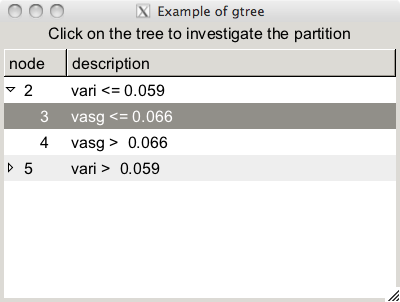
\includegraphics[width=.5\textwidth]{ex-gWidgets-gtree}
  \caption{GUI to explore return value of a model fit by the \code{party}  package.}
  \label{fig:ex-gWidgets-gtree-party}
\end{figure}


We make a simple GUI to show the widget (Figure~\ref{fig:ex-gWidgets-gtree-party})
\begin{Schunk}
\begin{Sinput}
 w <- gwindow("Example of gtree")
 g <- ggroup(cont=w, horizontal=FALSE)
 l <- glabel("Click on the tree to investigate the partition", 
             cont=g)
 tr <- gtree(offspring, cont=g, expand=TRUE)
\end{Sinput}
\end{Schunk}

A single click is used to expand the tree, here we create a binding to
a double click event to create a basic graphic. The \pkg{party}
vignette shows how to make more complicated -- and meaningful --
graphics for this model fit.
\begin{Schunk}
\begin{Sinput}
 addHandlerDoubleclick(tr, handler=function(h,...) {
   node <- as.numeric(svalue(h$obj))
   if(nodes(gt, node)[[1]]$terminal) {   # if terminal plot
     weights <- as.logical(nodes(gt,node)[[1]]$weights)
     plot(response(gt)[weights, ])
   }})
\end{Sinput}
\end{Schunk}
\end{example}

\section{Selecting from the file system}
\label{sec:gWidgets-selecting-from-file}

The \constructor{gfile} dialog allows one to select a file or directory
from the file system. This is a modal dialog, which returns the name
of the selected file or directory. The \constructor{gfilebrowse}
constructor creates a widget that has a button that allows the user to
initiate this selection.  

The selection type is specified by the \code{type} argument with
values of \code{open}, to select an existing file; \code{save} to
select a file to write to; and \code{selectdir} to select a
directory. For \code{RGtk2}, the \argument{filter}{gfile} argument can
be used to narrow the listed files. The dialog returns the path of the
file, or \code{NA} if the dialog was canceled. One can also specify a
handler to the constructor to call on the file or directory name. The
component \code{file} of the first argument to the handler contains
the file name.

\begin{Schunk}
\begin{Sinput}
 if(!is.na(tmp <- gfile())) 
   source(tmp)
 ## or
 gfile(handler=function(h,...) {
   if(!is.na(h$file))
     source(h$file) 
 })   
\end{Sinput}
\end{Schunk}
%$


\subsection{Selecting a date}
\label{sec:gWidgets-selecting-date}

The \constructor{gcalendar} constructor returns a widget that can be
used to select a date if the underlying toolkit supports such a widget
or a text edit box to allow the user to enter a date. The argument
\argument{text}{gcalendar} arugment can used to specify the initial
text. The \argument{format}{gcalendar} is used to specify the format
of the date.

The methods for the widget inherit from \code{gedit}. In particular,
the \method{svalue}{gcalendar} method returns the text in the text box
as a character vector formatted by the value specified by the
\argument{format}{gcalendar} argument. To return a value of a
different class, pass a function, such as \code{as.Date} to the
\argument{coerce.with}{gcalendar} argument.


\section{Display of graphics}
\label{sec:gWidgets-display-grapics}

\subsection{Displaying icons and images store in files}
\label{sec:gWidgets-displ-icons-imag}

The \pkg{gWidgets} package provides a few stock icons, that can be
added to various GUI components. A list of the defined stock icons is
returned by the function \code{getStockIcons}. The names attribute
defines the valid stock icon names.  For \pkg{gWidgetsRGtk2}, the size
of a stock icon can be adjusted through the \argument{size}{gimage}
argument, with a value from \qcode{menu}, \qcode{small\_toolbar},
\qcode{large\_toolbar}, \qcode{button}, or \qcode{dialog}.

Other Graphic files and the stock icons can be displayed by the
\constructor{gimage} widget. (Not all file types may be displayed by
each toolkit, in particular \pkg{gWidgetstcltk} can only display gif,
ppm, and xbm files.)  The file to display is specified through the
\argument{filename}{gimage} argument of the constructor. This value is
combined with that of the \argument{dirname}{gimage} argument to
specify the file path.  Stock icons, can be specified by using their
name for the \code{filename} argument and the character string
\code{"stock"} for the \code{dirname} argument.


%% methods

The \method{svalue\ASSIGN}{gimage} method can be used to change the
graphics file. In this case, a full path name is specified, or the
stock icon name.


More stock icon names may be added through the function
\code{addStockIcons}. This function requires a vector of stock icon
names and a vector of corresponding file paths, and is illustrated in
the example.

%% handlers
The default handler is called on a click event.

The \constructor{gsvg} constructor is similar, but allows one to
display SVG files, as produced by the \function{svg} driver, say. It
currently is only available for \pkg{gWidgetsQt}.

\begin{example}{Adding and using stock icons}{ex-gWidgets-stock-icons}
This example shows how to add to the available stock icons and use
\code{gimage} to display them. It creates a table to select a color
from, as an alternative to a more complicated color chooser
dialog. Under \pkg{gWidgetstcltk} the image files would need to be
converted to \code{gif} format, as \code{png} format is not a natively
supported image type.

We begin by defining 16 arbitrary colors.

\begin{Schunk}
\begin{Sinput}
 someColors <- c("black", "red", "blue", "brown",
                 "green", "yellow", "purple",
                 paste("grey", seq(10,90,by=10), sep=""))
\end{Sinput}
\end{Schunk}

This is the function that is used to create an icon file. We use some
low-level \pkg{grid} functions to draw the image to a png file.
\begin{Schunk}
\begin{Sinput}
 require(grid)
 iconDir <- tempdir(); iconSize <- 16;
 makeColorIcon <- function(i) {
   filename <- paste(iconDir, "/color-", i, ".png",
                     sep="", collapse="")
   png(file=filename, width=iconSize, height=iconSize)
   grid.newpage()
   grid.draw(rectGrob(gp=gpar(fill=i)))
   dev.off()
   return(filename)
 }
\end{Sinput}
\end{Schunk}

To add icons, we need to define the stock names and the file paths for
\code{addStockIcons}.

\begin{Schunk}
\begin{Sinput}
 icons <- sapply(someColors, makeColorIcon)
 iconNames <- paste("color-", someColors, sep="")
 QT <- addStockIcons(iconNames, icons)
\end{Sinput}
\end{Schunk}

We use a table layout to show the 16 colors. As an illustration of
assigning a handler for a click event, we assign one that returns the
corresponding stock icon name.

\begin{Schunk}
\begin{Sinput}
 w <- gwindow("Icon example")
 f <- function(h,...) print(h$action)
 tbl <- glayout(cont=w, spacing=0)
 for(i in 1:4) {
   for(j in 1:4) {
     ind <- (i - 1) * 4 + j
     tbl[i,j] <- gimage(icons[ind], handler=f, 
                        action=iconNames[ind], cont=tbl)
   }
 }
\end{Sinput}
\end{Schunk}
\end{example}

\subsection{A graphics device}
\label{sec:gWidgets-graphics-device}

Some toolkits support an embeddable graphics device (\pkg{RGtk2}
through \pkg{cairoDevice}). In which case, the \constructor{ggraphics}
constructor produces a widget that can be added to a container. The
arguments \argument{width}{ggraphics}, \argument{height}{ggraphics},
\argument{dpi}{ggraphics}, \argument{ps}{ggraphics} are similar to
other graphics devices.

The \constructor{ggraphicsnotebook} creates a notebook that allows the
user to easily navigate multiple graphics devices.


%%% 
\begin{example}{A GUI to explore a data set}{ex-gWidgets-baseball}
\begin{Schunk}
\begin{Soutput}
The  hash  package provided by:
                            _       _        
  ___  _ __   ___ _ __   __| | __ _| |_ __ _ 
 / _ \| '_ \ / _ \ '_ \ / _` |/ _' | __/ _' |
| (_) | |_) |  __/ | | | (_| | (_| | || (_| |
 \___/| .__/ \___|_| |_|\__,_|\__,_|\__\__,_|
      |_|   http://www.opendatagroup.com      
\end{Soutput}
\end{Schunk}

\begin{figure}
  \centering
  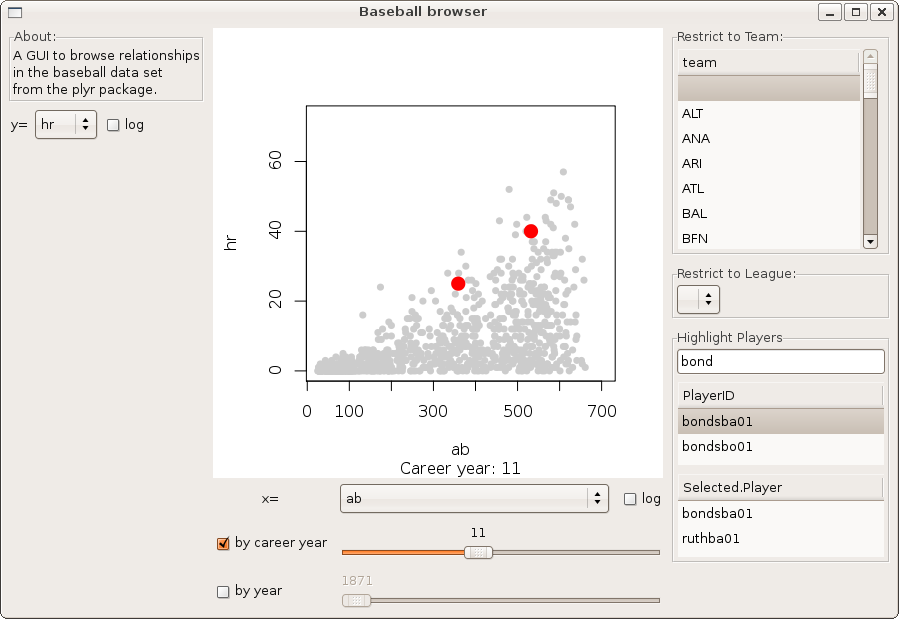
\includegraphics[width=.8\textwidth]{fig-gWidgets-baseball-gui.png}
  \caption{A \pkg{RGtk2} GUI for exploring the \code{baseball} data set of the \code{plyr} package. One can subset by year or career year through the slider widgets.}
  \label{fig:ex-gWidgets-baseball}
\end{figure}

This example creates a GUI to explore the \code{baseball} data set of
the \pkg{plyr} package.  The baseball data set contains information by
year for players who had 15-year or longer careers. Several
interesting things can be seen by looking at specific players, such as
Babe Ruth (coded \code{ruthba01}) or Barry Bonds (\code{bondsba01}).
Before beginning, we follow an example from the \pkg{plyr} package to create a
new variable to hold the career year of a player.
\begin{Schunk}
\begin{Sinput}
 data(baseball, package="plyr")
 calc <- function(df) 
   transform(df,
             cyear = year - min(year),
             cpercent = (year - min(year))/(max(year) - min(year)))
 b <- ddply(baseball, .(id), calc)
 b <- subset(b, ab >= 25) 
 nVars <- names(b)[-c(1:5,23:24)]    # numeric variables
\end{Sinput}
\end{Schunk}

This example uses the \pkg{hash} package to store our data and an environment to store our widgets.
\begin{Schunk}
\begin{Sinput}
 require(hash)
 dat <- hash()
 e <- new.env()
\end{Sinput}
\end{Schunk}

The following function transfers values from the GUI to our data
store, \code{dat}, returning \code{TRUE} if all goes well. The widgets
are all stored in an environment, \code{e} below, using names which
are again used as keys to the hash. We also define a function
\code{plotIt} to produce a graphic based on the current state of the
data store, but don't reproduce it here.
\begin{Schunk}
\begin{Sinput}
 transferData <- function() {
   out <- try(sapply(e, svalue, drop=TRUE), silent=TRUE)
   if(inherits(out,"try-error"))
     return(FALSE)
   dat[[names(out)]] <- out              # hash keys
   dat$id <- e$id[]                      # not svalue
   return(TRUE)                          # works!
 }
\end{Sinput}
\end{Schunk}


We now create a GUI so that the user can select which graphic to
make. Our GUI will have a main plot window to show a scatter plot, and
controls to adjust the variables that are plotted, and to filter the cases
considered.

Our layout will use box containers to split the top-level window into
three panes. The middle one holds the graphic, so we set it to
\code{expand} when the window is resized.
\begin{Schunk}
\begin{Sinput}
 w <- gwindow("Baseball browser", visible=FALSE)
 g <-  ggroup(cont=w, horizontal=TRUE)
 lp <- ggroup(cont=g, horizontal=FALSE)
 cp <- ggroup(cont=g, horizontal=FALSE, expand=TRUE)
 rp <- ggroup(cont=g, horizontal=FALSE, spacing=10)
\end{Sinput}
\end{Schunk}

The left panel holds a short description and a combobox to select the $y$-variable plotted.
\begin{Schunk}
\begin{Sinput}
 f <- gframe("About:", cont=lp)
 l <- glabel(paste("A GUI to browse relationships",
              "in the baseball data set",
              "from the plyr package.",
              sep="\n"),
        cont=f)
 g1 <- ggroup(cont=lp)
 l <- glabel("y=", cont=g1)
 e$y <- gcombobox(nVars, selected=4, cont=g1)
 e$ylog <- gcheckbox("log", checked=FALSE, cont=g1)
\end{Sinput}
\end{Schunk}

The center panel holds the \code{ggraphics} object, along wtih controls
to select the $x$ variable. As well, we add controls to filter out the
display by either the year a player played and/or their career year. A \code{gtable} instance is used for layout.
\begin{Schunk}
\begin{Sinput}
 gg <- ggraphics(cont=cp)
 tbl <- glayout(cont=cp)
 tbl[1,1] <- "x="
 tbl[1,2, expand=TRUE] <- (e$x <- gcombobox(nVars, selected=2, 
            cont=tbl))
 tbl[1,3] <- (e$xlog <- gcheckbox("log", checked=FALSE, 
                                  cont=tbl))
 ##
 tbl[2,1] <- (e$doCareerYear <- gcheckbox("by career year", 
                                          checked=TRUE, cont=tbl))
 tbl[2,2:3, expand=TRUE] <- (e$cyear <- 
              gslider(min(b$cyear), max(b$cyear), by=1, cont=tbl))
 enabled(e$cyear) <- TRUE
 ##
 tbl[3,1] <- (e$doYear <- gcheckbox("by year", 
                                    checked=FALSE, cont=tbl))
 tbl[3,2:3, expand=TRUE] <- (e$year <- 
              gslider(min(b$year), max(b$year), by=1, cont=tbl))
 enabled(e$year) <- FALSE
\end{Sinput}
\end{Schunk}

The right panel includes a few means to filter the display of
values. We use a simple \code{gtable} widget to allow the user to
restrict the display to one or more teams. A combobox allows the user
to restrict to one of the historic leagues. To allow certain players
to stand out, a compound widget is made using a \code{gedit} object to
filter values, a \code{gtable} object to show all possible IDs, and a
\code{gtable} object to show the selected IDs to highlight. Frames are
used to visually combine these controls.
\begin{Schunk}
\begin{Sinput}
 rpWidth <- 200
 f <- gframe("Restrict to Team:", cont = rp)
 teams <- data.frame(team=c("", sort(unique(b$team))), 
                     stringsAsFactors=FALSE)
 e$team <- gtable(teams, cont=f, multiple=TRUE, width=rpWidth)
 size(e$team) <- c(200,200)
 svalue(e$team, index=TRUE) <- 1
 ##
 f <- gframe("Restrict to League:", cont=rp)
 leagues <- names(table(b$lg))[-1]       # drop ""
 e$lg <- gcombobox(c("", leagues), cont=f)
 ##
 f <- gframe("Highlight Players", horizontal=FALSE, cont=rp)
 searchPlayer <- gedit("", cont=f)
 listPlayers <- gtable(data.frame("PlayerID"=unique(b$id), 
                                  stringsAsFactors=FALSE),
                       filter.FUN="manual", cont=f)
 e$id <- gtable(data.frame("Selected Player"=character(0), 
                           stringsAsFactors=FALSE), cont=f)
\end{Sinput}
\end{Schunk}

We define several handlers to make the GUI responsive to user
output. Rather than write an \code{updateUI} function to update the
GUI at periodic intervals, we use an event-driven model. These first
two handlers, simply toggle whether the user can control the display
by year or career year.
\begin{Schunk}
\begin{Sinput}
 f <- function(h,...) {
   val <- ifelse(svalue(h$obj), TRUE, FALSE)
   enabled(h$action) <- val
 }
 addHandlerChanged(e$doYear, handler=f, action=e$year)
 addHandlerChanged(e$doCareerYear, handler=f, action=e$cyear)
\end{Sinput}
\end{Schunk}
This next handler updates the graphic when any of several widgets is changed.
\begin{Schunk}
\begin{Sinput}
 f <- function(h, ...) transferdata() && plotIt()
 QT <- sapply(list(e$x, e$xlog, e$y, e$ylog, e$year, e$cyear,
                   e$doYear, e$doCareerYear, e$lg), 
              function(i) addHandlerChanged(i, handler=f))
\end{Sinput}
\end{Schunk}

For \code{gtable} objects, it is more natural here to bind to a single
mouse click, rather than the default double click.

\begin{Schunk}
\begin{Sinput}
 QT <- sapply(list(e$team, e$id), function(i)
        addHandlerClicked(i, handler=function(h, ...) 
                          transferData() && plotIt()))
\end{Sinput}
\end{Schunk}
These handlers are used to select the  IDs to highlight.
\begin{Schunk}
\begin{Sinput}
 addHandlerKeystroke(searchPlayer, handler=function(h, ...) {
   cur <- svalue(h$obj)
   ind <- grep(cur, unique(b$id))
   tmp <- rep(FALSE, length(unique(b$id)))
   if(length(ind) > 0) {
     tmp[ind] <- TRUE
     visible(listPlayers) <- tmp
   } else if(grepl("^\\s$", cur)) {
     visible(listPlayers) <- !tmp
   } else {
     visible(listPlayers) <- tmp
   }
 })
 addHandlerChanged(listPlayers,handler=function(h, ...) {
   val <- svalue(h$obj)
   e$id[] <- sort(c(val, e$id[]))
 })
 addHandlerChanged(e$id, handler=function(h, ...) {
   val <- svalue(h$obj)
   cur <- e$id[]
   e$id[] <- setdiff(cur, val)
 })
\end{Sinput}
\end{Schunk}

Finally, we implement functionality similar to the \code{locator}
function for the graphic. This handler labels the point nearest to a mouse click in
the plot area.
\begin{Schunk}
\begin{Sinput}
 distance <- function(x,y)  {
   ds <- apply(y, 1, function(i) sum((x-i)^2))
   ds[is.na(ds)] <- max(ds, na.rm=TRUE)
   ds
 }
 addHandlerClicked(gg, function(h,...) {
   x <- c(h$x, h$y)
   ds <- distance(x, curdf[,2:3])
   ind <- which(ds == min(ds))
   ids <- curdf[ind, 1]
   points(y[ind,1], y[ind,2], cex=2, pch=16, col="blue")
   text(y[ind,1], y[ind,2], label=ids, adj=c(-.25,0))
 })
\end{Sinput}
\end{Schunk}

To end, we show the GUI and initialize the plot.
\begin{Schunk}
\begin{Sinput}
 visible(w) <- TRUE
 QT <- transferData() && plotIt()
\end{Sinput}
\end{Schunk}

The \pkg{traitr} package, an add on for \pkg{gWidgets}, can simplify
the construction of such GUIs. The package vignette provides an example.
\end{example}


\section{Dialogs}
\label{sec:gWidgets-modal-dialogs}

The \pkg{gWidgets} package provides a few constructors to quickly make
some basic  dialogs for showing messages or gathering
information. Mostly these are modal dialogs that take control of the
eventloop, not allowing any other part of the GUI to be active for
programmatic interaction. As such, the constructors do not return an
object to manipulate through its methods, but rather the value of the
dialog specified by the user. Hence, they are used differently than
other constructors. For example, the \code{gfile} dialog, previously described, is
a modal dialog that pops up a means to select a file returning
the selected file path or \code{NA}.


\begin{table}
\centering
\label{tab:gWidgets-basic-dialogs}
\caption{Table of constructors for basic dialogs in \pkg{gWidgets}}
\begin{tabular}{@{}lp{0.7\textwidth}@{}}
\toprule

Constructor&Description\\
\midrule
\constructor{gfile}&File and directory selection dialog\\\constructor{gmessage}&Dialog to show a message\\\constructor{galert}&Unobtrusive (non-modal) dialog to show a message\\\constructor{gconfirm}&Confirmation dialog\\\constructor{ginput}&Dialog allowing user input\\\constructor{gbasicdialog}&Flexible modal dialog
\\ \bottomrule
\end{tabular}
\end{table}% \begin{table}
%   \centering
%  \begin{tabular}{l@{\quad}p{.75\textwidth}}
% %   \toprule
%     \constructor{gfile} & File and directory selection dialog\\
%     \constructor{gmessage} & Dialog to show a message\\
%     \constructor{galert} & Unobtrusive (non-modal) dialog to show a message\\
%     \constructor{gconfirm} & Confirmation dialog\\
%     \constructor{ginput} & Dialog allowing user input\\
%     \constructor{gbasicdialog} & Flexible modal dialog \\
%     \bottomrule
%   \end{tabular}
%   \caption{Table of basic dialogs in \pkg{gWidgets}}
%   \label{tab:gWidgets-modal-dialogs}
% \end{table}

Most of these dialogs pop up a window with a common appearance. The
constructors have arguments \argument{message}{gmessage} for a
message; \argument{title}{gmessage} for the window title; and
\argument{icon}{gmessage} to specify an icon, whose value is one of
\qcode{info}, \qcode{warning}, \qcode{error}, or
\qcode{question}. Buttons will appear at the bottom of the dialog,
and are determined by choice of the constructor. The
\argument{parent}{gmessage} argument will place the dialog near the
\pkg{gWidgets} instance specified. Otherwise, placement will be
controlled by the window manager.

The dialogs, except for \code{galert}, have the standard
\code{handler} and \code{action} arguments, for calling a handler, but
typically it is easier to use the return value when programming.

\paragraph{A message dialog}
The simplest dialog is produced by \code{gmessage}, which is used to
display a message. The user has a cancel button to dismiss the dialog.

\paragraph{An alert dialog}
The \code{galert} dialog is similar to \code{gmessage} only it is meant
to be less obtrusive, so it is non-modal. It does not take the focus and vanishes after a time delay.

\paragraph{A confirmation dialog}
The constructor \constructor{gconfirm} produces a dialog that allows
the user to confirm the message. This dialog returns \code{TRUE} or
\code{FALSE} depending on the user's selection.


\paragraph{An input dialog}
The \constructor{ginput} constructor produces a dialog which allows
the user to input a single line of text. If the user confirms the
dialog, the value of the string is returned, otherwise if the user
cancels the dialog through the button a value of \code{NA} is returned.




\paragraph{A basic dialog}
The \constructor{gbasicdialog} constructor allows one to place an
arbirary widget within a modal window with \kbd{OK} and
\kbd{Cancel}. The handler, if specified, will be called if the user
clicks the \kbd{OK} button. This allows users to create their own
modal dialogs.

As with the others, the argument \argument{title}{gbasicdialog} is
used to specify the window title, but there is no \code{icon} or
\code{message} arguments, as there is no standard appearance. Rather,
the \argument{widget}{gbasicdialog} argument specifies a widget to
pack into the dialog. This can be a simple control, or a container
containing other widgets. 

As with \code{gconfirm}, this widget returns \code{TRUE} or
\code{FALSE} depending on the user's selection. To do something more complicated than \code{gconfirm}, a handler should be specified at construction. If the user selects
\kbd{OK}, the handler, if specified, is called before the value \code{TRUE}
is returned. 

This dialog is called a bit awkwardly, to allow it to work when controls need a
parent container specified at construction time (e.g., \pkg{tcltk}). The construction is in
three stages: an initial call to \code{gbasicdialog} to return a container which is used as
the parent container for a child component; a construction of the dialog; then a call to the
\code{visible} method on the dialog with \code{set=TRUE} value (not though \code{visible(obj) \ASSIGN\/ TRUE}).


\begin{example}{Modal dialogs}{ex-gWidgets-modal-dialogs}
The basic message dialog requires just the first argument.
\begin{Schunk}
\begin{Sinput}
 gmessage("Message goes here", title="example dialog")
\end{Sinput}
\end{Schunk}

Here we use the question icon for a confirmation dialog, as the message is a question.
\begin{Schunk}
\begin{Sinput}
 ret <- gconfirm("Really delete file?", icon="question")
\end{Sinput}
\end{Schunk}

This illustrates how to use the return value.
\begin{Schunk}
\begin{Sinput}
 ret <- ginput("Enter your name", icon="info")
 if(!is.na(ret)) 
   cat("Hello",ret,"\n")
\end{Sinput}
\end{Schunk}

The \code{gbasicdialog} constructor can be used to make modal
dialogs. This example will force the user to
select a color before proceeding with anything else. 
\begin{Schunk}
\begin{Sinput}
 ## create a parent container
 dlg <- gbasicdialog("Pick a color", handler = 
                     function(h,...) print(svalue(widget)))
 ## create the dialog using dlg as the parent container
 widget <- gtable(colors(), cont = dlg)
 ## show the modal dialog (not visible(dlg) <- TRUE)
 visible(dlg, set=TRUE)    
\end{Sinput}
\end{Schunk}

\end{example}
















\section{\pkg{gWidgets}: Compound widgets}
\label{sec:compound-widgets}
The \pkg{gWidgets} package provides some \R\/ specific widgets for
producing GUIs. Table~\ref{tab:gWidgets-compound-widgets} lists them.


\begin{table}
\centering
\label{tab:gWidgets-compound-widgets}
\caption{Table of constructors for compound widgets in \pkg{gWidgets}}
\begin{tabular}{@{}lp{0.7\textwidth}@{}}
\toprule

Constructor&Description\\
\midrule
\constructor{gvarbrowser}&GUI for browsing variables in the workspace\\\constructor{gcommandline}&Command line widget\\\constructor{gformlayout}&Uses list to specify layout of a GUI\\\constructor{ggenericwidget}&Creates a GUI for a function based on its formal arguments or a defining list
\\ \bottomrule
\end{tabular}
\end{table}
% \begin{table}
%   \centering
%   \begin{tabular}{l@{\quad}p{.75\textwidth}}
% %    \toprule
%     \constructor{gcommandline} & Command line widget\\ 
%     \constructor{gvarbrowser} & GUI for browsing variables in the workspace\\
% %    \constructor{gdfnotebook} & A notebook of data frames\\
% %    \constructor{ggraphicsnotebook} & A notebook for graphics objects\\
%     \constructor{ghelp} & GUI for a help page\\
%     \constructor{ghelpbrowser} & A help browser\\
%     \constructor{gformlayout} & Uses list to specify layout of a GUI\\
%     \constructor{ggenericwidget} & Creates a GUI for a function based
%     on its formal arguments or a defining list\\
%     \bottomrule
%   \end{tabular}
%   \caption{Table of compound widgets provided by \pkg{gWidgets}}
%   \label{tab:gWidgets-compound-widgets}
% \end{table}


\subsection{Workspace browser}
\label{sec:gWidgets-workspace-browser}

A workspace browser is constructed by \code{gvarbrowser}, providing a
means to browse and select the objects in the current global environment. The
quality of the implementation varies depending on the toolkit. The
default \code{handler} object calls \code{do.call} on the object for
the function specified through the \argument{action}{gvarbrowser}
argument. The default is to print a \code{summary} of the object. This
handler is called on a double click. A single click is used for
selection. The name of the currently selected value is returned by the
\method{svalue}{gvarbrowser} method.

% \subsection{Help browser}
% \label{sec:gWidgets-help-browser}

% The \constructor{ghelp} constructor produces a widget for showing help
% pages using a notebook container. This widget does not use the html
% help pages or the chm help pages, so it may not work for all operating
% systems. (For Windows, the help browser of the GUI is much better
% anyways.) To add a help page, the \method{add}{ghelp} method is used,
% where the \code{value} argument describes the desired page. This can
% be a character string containing the topic, a character string of the
% form \code{package:::topic} to specify the package, or a list with
% named components \code{package} and \code{topic}.  The
% \method{dispose}{ghelp} method of notebooks can be used to remove the
% current tab.

% The \constructor{ghelpbrowser} constructor produces a stand-alone
% GUI for displaying help pages, running examples from the help pages or
% opening vignettes provided by the package. This GUI provides its own
% top-level window and does not return a value for which methods are defined.



\subsection{Command line widget}
\label{sec:gWidgets-command-line-widget}

A simple command line widget is created by the
\constructor{gcommandline} constructor. This is not meant as a
replacement for \R's typical commandlines, but is provided for
lightweight usage. A text box allows users to to type in \R\/
commands. The programmer may issue commands to be evaluated and
displayed through the \method{svalue\ASSIGN}{gcommandline} method. The
\code{value} assigned is a character string holding the commands. If
there is a names attribute, the results will be assigned to a variable
in the global workspace with that name. The \code{svalue} and \code{[}
methods return the command history.

\subsection{Simplifying creation of dialogs}
\label{sec:gWidgets-designing-forms}

The \pkg{gWidgets} package has two means to simpify the creation of
GUIs. The \code{gformlayout} constructor takes a list defining a
layout and produces a GUI, the \code{ggenericwidget} constructor can
take a function name and produce a GUI based on the formal arguments
of the function. This too uses a list, that can be modified by the
user before the GUI is constructed. 

\subsubsection{Laying out a form}
\label{sec:gWidgets-laying-out-form}

The \constructor{gformlayout} constructor takes a list defining a
layout and creates the specified widgets. The design borrows from the
\code{extjs} javascript libraries for web programming, where a similar
function can be used to specify the layout of web forms. Several
toolkits have a means to specify a layout using XML (eg. \GTK's
Builder and \Qt's assistant), this implementation uses a list,
assuming this is more familiar to the \R\/ user. By defining the
layout ahead of time, pieces of the layout can be recycled for other
layouts.


To define the layout, each component is specified using a list with
named components. The component \code{type} indicates what component
to be created, as a string. This can be a the name of a container
constructor, a widget constructor or the special value
\code{"fieldset"}. Field sets are used to group a set of common
controls. If the component \code{name} is specified, then the
component that is created will be stored in the list returned by the
\code{[} method.

The \code{label} component can be specified to
add a descriptive label to the layout. When used, the component
\code{label.pos} can be tale a value \code{"top"} to have the label
on top of the widget, or \code{"side"} to place the label on the side
(the default positioning). The \code{label.font} component can be used
to specify the label's font properties using a label's \meth{font\ASSIGN} method.

If the type is a container or fieldset, then the \code{children}
component is a list whose components specify the children as
above. Except for fieldsets, these children can contain other
containers or components. Fieldsets only allow components as children.

Whether a widget is enabled or not can be controlled by specifying
values for \code{depends.on}, \code{depends.FUN}, and
\code{depends.signal}. If the component \code{depends.on} specifies
the name of a previous component, then the function \code{depends.FUN}
will be consulted when the signal specified by \code{depends.signal}
is emitted. This uses the \code{addHandlerXXX} names with a default
value of \code{addHandlerChanged}. The \code{depends.FUN} function has
a single argument consisting of the value returned by \code{svalue}
when called on the widget specified through \code{depends.on}. This
function should return a logical indicating if the widget is enabled
or not.

\paragraph{Methods}
The constructor returns an object with a few methods. The
\method{[}{gformlayout} method will return a list with
components being the widgets that were named in the defining list. The
\method{svalue}{gformlayout} method simply applies the \code{svalue}
method for each component of the list returned by the \code{[}
method. The \method{names}{gformlayout} method returns the names of the widgets in the list.


\begin{example}{The \code{gformlayout} constructor}{ex-gWidgets-gformlayou}
This example uses \code{gformlayout} to make a GUI for a $t$-test (Figure~\ref{fig:ex-gWidgets-formlayout}). The
first task is to define the list that will set up the GUI. We do this
in pieces. This first piece will define the part of the GUI where the
null and alternative hypotheses are specified. The null is specified
as a numeric value with a default of 0. We use the \code{gedit} widget
which by default will return a character value, so the
\code{coerce.with} argument is specified. For the alternative, this
requires a selection for just 3 possibilities, so a combo box is
employed.
\begin{figure}
  \centering
  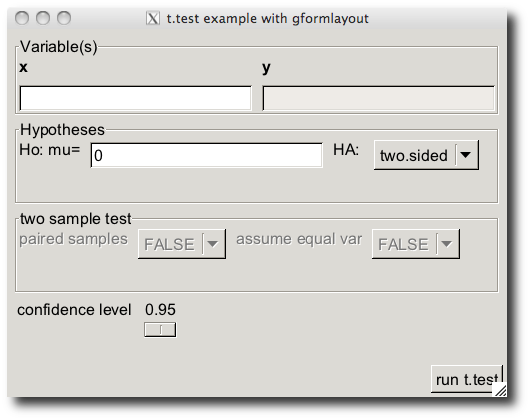
\includegraphics[width=.65\textwidth]{ex-gWidgets-formlayout}
  \caption{A dialog to collect arguments for a $t$-test made with \code{gformlayout}.}
  \label{fig:ex-gWidgets-formlayout}
\end{figure}


\begin{Schunk}
\begin{Sinput}
 hypotheses <- 
   list(type = "fieldset",
        label = "Hypotheses",
        columns = 2, 
        children = list(
          list(type="gedit",                            
               name="mu", label="Ho: mu=",
               text="0", coerce.with=as.numeric),
          
          list(type="gcombobox",
               name="alternative", label="HA: ",
               items=c("two.sided","less","greater")
               )))
\end{Sinput}
\end{Schunk}

Basic usage of the \code{t.test} function allows for an \code{x}, or
\code{x} and \code{y} variable to be specified. Here we disable the
\code{y} variable until the \code{x} one has been entered. The
\code{addHandlerChanged} method is called when the enter key is
pressed after the \code{x} value is specified.

\begin{Schunk}
\begin{Sinput}
 variables <- 
   list(type="fieldset",
        columns = 2,
        label = "Variable(s)",
        label.pos = "top",
        label.font = c(weight="bold"),
        children = list(
          list(type = "gedit",
               name = "x", label = "x",
               text = ""),
          list(type = "gedit",
               name = "y", label = "y",
               text = "",
               depends.on = "x",
               depends.FUN = function(value) nchar(value) > 0,
               depends.signal = "addHandlerChanged"
               )))
\end{Sinput}
\end{Schunk}

If a \code{y} value is specified, then the two-sample options make sense. This enables them dependent on that happening.

\begin{Schunk}
\begin{Sinput}
 two.sample <-  
   list(type = "fieldset",
        label = "two sample test",
        columns = 2,
        depends.on = "y",
        depends.FUN = function(value) nchar(value) > 0,
        depends.signal = "addHandlerChanged",                     
        children = list(
          list(type = "gcombobox",
               name = "paired", label = "paired samples",
               items = c(FALSE, TRUE)
               ),
          list(type = "gcombobox",
               name = "var.equal", label = "assume equal var",
               items = c(FALSE, TRUE)
               )))
\end{Sinput}
\end{Schunk}

The confidence interval specification is specified using a slider for variety.

\begin{Schunk}
\begin{Sinput}
 conf.level <- 
   list(type = "fieldset",
        columns = 1,
        children = list(
          list(type = "gslider",
               name = "conf.level", label = "confidence level",
               from=0.5, to=1.0, by=.01, value=0.95
               )))
\end{Sinput}
\end{Schunk}
Finally, the constituent pieces are placed inside a box container.
\begin{Schunk}
\begin{Sinput}
 tTest <- list(type = "ggroup",
               horizontal = FALSE,
               children = list(
                 variables,
                 hypotheses,
                 two.sample,
                 conf.level
                 ))
\end{Sinput}
\end{Schunk}

The layout of the GUI is primarily done by the \code{gformlayout}
call. The following just places the values in a top-level window and adds a
button to initiate the call to \code{t.test}.

\begin{Schunk}
\begin{Sinput}
 w <- gwindow("t.test example with gformlayout")
 g <- ggroup(horizontal=FALSE, cont=w)
 fl <- gformlayout(tTest, cont=g, expand=TRUE)
 bg <- ggroup(cont=g)
 addSpring(bg)
 b <- gbutton("Run t.test", cont=bg)
\end{Sinput}
\end{Schunk}

The handler is very simple, as the names chosen match the argument
names of \code{t.test}, so the list returned by the \meth{svalue}
method can be used with \code{do.call}. The only needed adjustment is
for the one-sample case.

\begin{Schunk}
\begin{Sinput}
 addHandlerChanged(b, function(h, ...) {
   out <- svalue(fl)
   out$x <- svalue(out$x) # turns text string into numbers
   if(out$y == "") {
     out$y <- out$paired <- NULL 
   } else {
    out$y <- svalue(out$y)
   }
   print(do.call("t.test", out))
 })
\end{Sinput}
\end{Schunk}

\end{example}

\subsubsection{Automatically creating a GUI}
\label{sec:gWidgets-autom-creat-gui}

The \constructor{ggenericwidget} constructor can create a basic GUI
for a function using the function's formal arguments as a guide for
the proper widget to use to collect values for an argument of the
function. The \pkg{fgui} package provides a similar function using
just the \pkg{tcltk} package, only it improves \code{ggenericwidget} by
parsing the function's help page.

The implementation actually has two stages, the first creates a list
specifying the layout of the GUI and the second a call to layout the
GUI. This list is different from that used by \code{gformlayout}. It
does not provide as much flexibility and is described in the help page
for \code{ggenericwidget}. This list can be edited if desired and then
used directly.

The formal arguments of an S3 method may be different from those of
its generic. For instance, those for the \code{t.test} generic are
much different (and less useful for this purpose) than the
\code{t.test.default} method for numeric values for \code{x}. Knowing
this, a useful GUI can be quickly created for the \code{t.test} with
the commands:
\begin{Schunk}
\begin{Sinput}
 w <- gwindow("t.test through ggenericwidget")
 f <- stats:::t.test.default; 
 widget <- ggenericwidget("f", cont=w)
\end{Sinput}
\end{Schunk}



\XXX{Need to have an example with drag and drop}


%\section{End of chapter notes}
%\label{sec:gWidgets:eoc}








%% RGtk2
%%\part{The \pkg{RGtk2} package}
\label{chap:RGtk2}

% XXX- discuss GtkBin; which widgets have a window, which do not --image and label do not, and we mightwant them too,
%   modify_bg() only affects widgets that have an associated gtk.gdk.Window.
% > Widgets that do not have an associated window include .... gtk.Arrow,
% > gtk.Bin, gtk.Box, gtk.Button, gtk.CheckButton, gtk.Fixed , gtk.Image ,
% > gtk.Label , gtk.MenuItem , gtk.Notebook , gtk.Paned , gtk.RadioButton ,
% > gtk.Range , gtk.ScrolledWindow , gtk.Separator , gtk.Table , gtk.Toolbar ,
% > gtk.AspectFrame , gtk.Frame , gtk.VBox , gtk.HBox , gtk.VSeparator ,
% > gtk.HSeparator . These widgets can be added to a gtk.EventBox to overcome
% > this limitation.




%% RGtk2 chapter
\chapter{RGtk2: Overview}
%%\section{Introduction}
\label{sec:RGtk2-Introduction}
%% intorduction

%% Technical, but short beginning

As the name implies, the \pkg{RGtk2} package is an interface, or
binding, between \R\/ and \GTK, a mature, cross-platform GUI
toolkit. The letters \emph{GTK} stand for the \emph{GIMP ToolKit},
with the word \emph{GIMP} recording the origin of the library as part
of the GNU Image Manipulation Program. \pkg{GTK+} provides the same
widgets on every platform, though it can be customized to emulate
platform-specific look and feel. The library is written in
\proglang{C}, which facilitates access from languages like
\proglang{R} that are also implemented in \proglang{C}. \pkg{GTK+} is
licensed under the \textit{Lesser GNU Public License} (LGPL), while
\pkg{RGtk2} is under the \textit{GNU Public License} (GPL).
The package is available from the Comprehensive \proglang{R} Archive
Network (CRAN) at \url{http://CRAN.R-project.org/package=RGtk2}.

The name \pkg{RGtk2} also implies that there exists a package named
\pkg{RGtk}, which is indeed the case. The original \pkg{RGtk} is bound
to the previous generation of \pkg{GTK+}, version 1.2. \pkg{RGtk2} is
based on \pkg{GTK+ 2.0}, the current generation. This book covers
\pkg{RGtk2} specifically, although many of the fundamental features of
\pkg{RGtk2} are inherited from \pkg{RGtk}. 

\pkg{RGtk2} provides virtually all of the functionality in \GTK\/ to
the \R\/ programmer. In addition, \pkg{RGtk2} interfaces with several
other libraries in the \GTK\/ stack: Pango for font rendering; Cairo
for vector graphics; GdkPixbuf for image manipulation; GIO for
synchronous and asynchronous input/output for files and network
resources; ATK for accessible interfaces; and GDK, an abstraction over
the native windowing system, supporting either X11 or Windows. These
libraries are multi-platform and extensive and have been used for many
major projects, such as the Linux versions of Firefox and Open Office.

The API of each of these libraries is mapped to \R\/ in a way that is
consistent with \R\/ conventions and familiar to the \R\/
user. Much of the \pkg{RGtk2} API consists of autogenerated \R\/
functions that call into one of the underlying libraries. For
example, the \R\/ function \function{gtkContainerAdd} eventually calls
the C function \code{gtk\_container\_add}. The naming convention is
that the C name has its underscores removed and each following letter
capitalized (camelback style).

The full API for \GTK\/ is quite large, and complete documentation of
it is beyond our scope. However, the \GTK\/ documentation is
algorithmically converted into the \R\/ help format during the
generation of \pkg{RGtk2}. This conveniently allows the programmer to
refer to the appropriate documentation within an \R\/ session, without
having to consult a web page, such as
\url{http://library.gnome.org/devel/gtk/stable/}, which lists the
\proglang{C} API of the stable version of \GTK.

In this chapter, we give an overview of how \pkg{RGtk2} maps the
\GTK\/ API, including its classes, constructors, methods, properties,
signals and enumerations, to an \R-level API that is relatively
familiar to, and convenient for, an \R\/ user. 
% A simple GUI will be
% gradually constructed to demonstrate the API.

%%% ------- OOP --------------

\section{Synopsis of the \pkg{RGtk2} API}

Constructing a GUI with \pkg{RGtk2} generally proceeds by constructing
a widget and then configuring it by calling methods and setting
properties. Handlers are connected to signals, and the widget is
combined with other widgets to form the GUI. For example:
\begin{Schunk}
\begin{Sinput}
 button <- gtkButton("Click Me")
 button['image'] <- gtkImage(stock = "gtk-apply", size = "button")
 gSignalConnect(button, "clicked", function(x) message("Hello World!"))
 window <- gtkWindow(show = FALSE)
 window$add(button)
 window$showAll()
\end{Sinput}
\end{Schunk}
% 
Once one understands the syntax and themes of the above example, it is
only a matter of reading through the proceeding chapters and the
documentation to discover all of the widgets and their features. The
rest of this chapter will explain these basic components of the API.

\section{Objects and Classes}

In any toolkit, all widget types have functionality in common. For
example, they are all drawn on the screen in a consistent style. They
can be hidden and shown again. To formalize this relationship and to
simplify implementation by sharing code between widgets, \pkg{GTK+},
like many other toolkits, defines an inheritance hierarchy for its
widget types. In the parlance of object-oriented programming, each
type is represented by a \textit{class}.

For specifying the hierarchy, \pkg{GTK+} relies on \pkg{GObject}, a
\proglang{C} library that implements a class-based, single-inheritance
object-oriented system. A \pkg{GObject} class encapsulates behaviors
that all instances of the class share. Every class has at most one
parent through which it inherits the behaviors of its ancestors. A
subclass can override some specific inherited behaviors. The interface
defined by a class consists of constructors, methods, properties,
and signals. 

The type system supports reflection, so we can, for example, obtain a
list of the ancestors for a given class:
\begin{Schunk}
\begin{Sinput}
 gTypeGetAncestors("GtkWidget")
\end{Sinput}
\begin{Soutput}
[1] "GtkWidget"         "GtkObject"         "GInitiallyUnowned"
[4] "GObject"          
\end{Soutput}
\end{Schunk}
%
For those familiar with object-oriented programming in R, the returned
character vector could be interpreted as it were a class attribute on
an S3 object.

Single inheritance can be restrictive when a class performs multiple
roles in a program. To circumvent this, \pkg{GTK+} adopts the popular
concept of the \textit{interface}, which is essentially a contract
that specifies which methods, properties and signals a class must
implement. As with languages like Java and \proglang{C\#}, a class can
\textit{implement} multiple interfaces, and an interface can be
composed of other interfaces. An interface allows the programmer to
treat all instances of implementing classes in a similar way. However,
unlike class inheritance, the implementation of the methods,
properties and signals is not shared. For example, we list the
interfaces implemented by \class{GtkWidget}:
\begin{Schunk}
\begin{Sinput}
 gTypeGetInterfaces("GtkWidget")
\end{Sinput}
\begin{Soutput}
[1] "GtkBuildable"        "AtkImplementorIface"
\end{Soutput}
\end{Schunk}

We explain the constructors, methods, properties and signals of
classes and interfaces in the following sections and demonstrate them
in the construction of a simple ``Hello World'' GUI, shown in
Figure~\ref{fig:hello-world}. A more detailed and technical
explanation of \pkg{GObject} is available in
Section~\ref{sec:gobject-primer}.

\begin{figure}[h!tbp]
  \begin{center}
    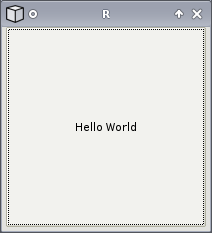
\includegraphics[width=2in]{hello-world.png}
    \caption{\label{fig:hello-world}``Hello World'' in GTK+. 
      A window containing a single button displaying a label with the text
      \code{Hello World}.}
  \end{center}
\end{figure}

\section{Constructors}

The next few sections will contribute to a unifying example that
displays a button in a window. When clicked, the button will print a
message to the R console. The first step in our example is to create a
top-level window to contain our GUI.  Creating an instance of a GTK\/
widget requires calling a single \R\/ function, known as a
constructor. Following \R\/ conventions, the constructor for a class
has the same name as the class, except the first character is
lowercase. The following statement constructs an instance of the
\code{GtkWindow} class:
\begin{Schunk}
\begin{Sinput}
 window <- gtkWindow("toplevel", show = FALSE)
\end{Sinput}
\end{Schunk}
%
The first argument to the constructor for \code{GtkWindow} instructs
the window manager to treat the window as top-level.  The \code{show}
argument is the last argument for every widget constructor. It
indicates whether the widget should be made visible immediately after
construction.  The default value of \code{show} is \code{TRUE}. In
this case we want to defer showing the window until after we finish
constructing our simple GUI.

At the \GTK\/ level, a class usually has multiple constructors, each
implemented as a separate C function. In \pkg{RGtk2}, the names of
these functions all end with \code{New}. The ``meta'' constructor
\function{gtkWindow}, called above, automatically delegates to one of
the low-level constructors, based on the provided arguments.
We prefer these shorter, more flexible constructors, such as
\function{gtkWindow} or \function{gtkButton}, but note their
documentation is provided by the \R\/ package author and is in
addition to the formal API. These constructors can take many
arguments, and only some subsets of the arguments may be specified at
once. For example, this call
\begin{Schunk}
\begin{Sinput}
 gtkImage(stock = "gtk-apply", size = "button")
\end{Sinput}
\end{Schunk}
% 
uses only two arguments, \argument{stock}{gtkImage} and
\argument{size}{gtkImage}, which always must be specified
together. The entire signature is more complex:
\begin{Schunk}
\begin{Sinput}
 args(gtkImage)
\end{Sinput}
\begin{Soutput}
function (size, mask = NULL, pixmap = NULL, image = NULL, filename, 
    pixbuf = NULL, stock.id, icon.set, animation, icon, show = TRUE) 
NULL
\end{Soutput}
\end{Schunk}

A \GTK\/ object created by the \R\/ user has an \R-level object as its
proxy. Thus, \code{window} is a reference to a \class{GtkWindow}
instance. A reference object will not be copied before
modification. This is different from the behavior of most \R\/
objects. For example, calling \function{abs} on a numeric vector does
not change the value assigned to the original symbol:
\begin{Schunk}
\begin{Sinput}
 a <- -1
 abs(a)
\end{Sinput}
\begin{Soutput}
[1] 1
\end{Soutput}
\begin{Sinput}
 a
\end{Sinput}
\begin{Soutput}
[1] -1
\end{Soutput}
\end{Schunk}
% 
Setting the text label on our button, however, will change the
original value:
\begin{Schunk}
\begin{Sinput}
 gtkButtonSetLabel(button, "New text")
 gtkButtonGetLabel(button)
\end{Sinput}
\begin{Soutput}
[1] "New text"
\end{Soutput}
\end{Schunk}
% 
If this widget were displayed on the screen, the label would also be
updated.

The class hierarchy of an object is represented by the
\code{class} attribute. One interprets the attribute according to S3
conventions, so that the class names are in order from most to least
derived:
\begin{Schunk}
\begin{Sinput}
 class(window)
\end{Sinput}
\begin{Soutput}
[1] "GtkWindow"         "GtkBin"            "GtkContainer"     
[4] "GtkWidget"         "GtkObject"         "GInitiallyUnowned"
[7] "GObject"           "RGtkObject"       
\end{Soutput}
\end{Schunk}
%
We find that the \class{GtkWindow} class inherits methods,
properties, and signals from the \class{GtkBin}, \class{GtkContainer},
\class{GtkWidget}, \class{GtkObject}, \class{GInitiallyUnowned}, and
\class{GObject} classes. Every type of \pkg{GTK+} widget inherits from
the base \code{GtkWidget} class, which implements the general
characteristics shared by all widget classes, e.g., properties storing
the location and background color; methods for hiding, showing and
painting the widget. We can also query \code{window} for the
interfaces it implements:
\begin{Schunk}
\begin{Sinput}
 interface(window)
\end{Sinput}
\begin{Soutput}
[1] "GtkBuildable"        "AtkImplementorIface"
\end{Soutput}
\end{Schunk}

When the underlying \GTK\/ object is destroyed, i.e., deleted
from memory, the class of the proxy object is set to \class{<invalid>},
indicating that it can no longer be manipulated.

\section{Methods}

The next steps in our example are to create a ``Hello World'' button
and to place the button in the window that we have already
created. This depends on an understanding of how of one
programmatically manipulates widgets by invoking methods.  Methods are
functions that take an instance of their class as the first argument
and instruct the widget to perform an action.

Although class information is stored in the style of S3, \pkg{RGtk2}
introduces its own mechanism for method dispatch.  The call
\code{obj\$method(...)}  resolves to a function call
\code{f(obj,...)}. The function is found by looking for any function
that matches the pattern \emph{classNameMethodName}, the concatenation
of one of the names from \code{class(obj)} or \code{interface(obj)}
with the method name. The search begins with the interfaces and
proceeds through each character vector in order.

For instance, if \code{win} is a \function{gtkWindow} instance, then
to resolve the call \code{win\$add(widget)} \pkg{RGtk2} considers
\function{gtkBuildableAdd}, \function{atkImplementorIfaceAdd},
\function{gtkWindowAdd}, \function{gtkBinAdd} and finally finds
\function{gtkContainerAdd}, which is called as
\code{gtkContainerAdd(win, widget)}. The \method{\$}{GObject} method
for \pkg{RGtk2} objects does the work.

We take advantage of this convenience when we add the ``Hello World''
button to our window and set its size:
\begin{Schunk}
\begin{Sinput}
 button <- gtkButton("Hello World")
 window$add(button)
 window$setDefaultSize(200, 200)
\end{Sinput}
\end{Schunk}
%
The above code calls the \function{gtkContainerAdd} and
\function{gtkWindowSetDefaultSize} functions with less typing and less
demands on the memory of the user.

Understanding this mechanism allows us to add to the \pkg{RGtk2}
API. For instance, we can add to the button API with
\begin{Schunk}
\begin{Sinput}
 gtkButtonSayHello <- function(obj, target) 
   obj$setLabel(paste("Hello", target))
 button$sayHello("World")
 button$getLabel()
\end{Sinput}
\begin{Soutput}
[1] "Hello World"
\end{Soutput}
\end{Schunk}

%% common methods
Some common methods are inherited by most widgets, as they are defined
in the base \class{GtkWidget} class. These include the methods 
\method{show}{GtkWidget} to specify that the widget should be drawn;
\method{hide}{GtkWidget} to hide the widget until specified;
\method{destroy}{GtkWidget} to destroy a widget and clear up any
references to it; \method{getParent}{gtkWidget} to find the parent
container of the widget; \method{modifyBg}{GtkWidget} to modify the
background color of a widget; and \method{modifyFg}{GtkWidget} to
modify the foreground color.


\section{Properties}


%% --------- Properties ------------
The \GTK\/ API uses properties to store object state. Properties are
similar to R attributes and even more so to S4 slots. They are
inherited, typed, self-describing and encapsulated, so that an object
can intercept access to the underlying data. A list of properties
definitions belonging to the widget is returned by its
\method{getPropInfo}{GObject} method. Calling \function{names} on the
object returns the property names. Auto-completion of property names
is gained as a side effect.  For the button just defined, we can see
the first eight properties listed with:
\begin{Schunk}
\begin{Sinput}
 head(names(button), n=8)                 # or b$getPropInfo()
\end{Sinput}
\begin{Soutput}
[1] "use-action-appearance" "related-action"       
[3] "user-data"             "name"                 
[5] "parent"                "width-request"        
[7] "height-request"        "visible"              
\end{Soutput}
\end{Schunk}

Some common properties are: \code{parent}, to store the parent widget
(if any); \code{user-data}, which allows one to store arbitrary data
with the widget; and \code{sensitive}, to control whether a widget can
receive user events. 

There are a few different ways to access these properties. The methods
\method{get}{GObject} and \method{set}{GObject} get and set properties
of a widget, respectively. The set funtion treats the argument names
as the property names, and setting multiple properties at once is
supported. Here we add an icon to the top-left corner of our window
and set the title:
\begin{Schunk}
\begin{Sinput}
 image <- gdkPixbuf(filename = imagefile("rgtk-logo.gif"))[[1]]
 window$set(icon = image, title = "Hello World 1.0")
\end{Sinput}
\end{Schunk}

Additionally, most user-accessible properties have specific \code{get} and
\code{set} methods defined for them. For example, to set the title of
the window, we could have used the \method{setTitle}{GtkWindow} method
and verified the change with \method{getTitle}{GtkWindow}.
\begin{Schunk}
\begin{Sinput}
 window$setTitle("Hello World 1.0")
 window$getTitle()
\end{Sinput}
\begin{Soutput}
[1] "Hello World 1.0"
\end{Soutput}
\end{Schunk}

\pkg{RGtk2} provides the convenient and familiar \code{[} and
\code{[$<$-} methods to get and access the properties. In our example,
we might check the window to ensure that it is not yet visible:
\begin{Schunk}
\begin{Sinput}
 window["visible"]
\end{Sinput}
\begin{Soutput}
[1] FALSE
\end{Soutput}
\end{Schunk}
Finally, we can make our window visible by setting the ``visible'' property,
although calling \function{gtkWidgetShow} is more conventional:
\begin{Schunk}
\begin{Sinput}
 window["visible"] <- TRUE 
 window$show() # same effect
\end{Sinput}
\end{Schunk}

For ease of referencing the appropriate help pages, we tend to use the
full method name in the examples, although at times the move \R-like
vector notation will be used for commonly accessed properties.

%%% ------ Signals ----------

\section{Events and signals}

In \pkg{RGtk2}, a user action, such as a mouse click, key press or
drag and drop motion triggers the widget to emit a corresponding
signal.  A GUI can be made interactive by specifying a callback
function to be invoked upon the emission of a particular signal.

The signals provided by a class or interface are returned by the
function \function{gTypeGetSignals}. For example
\begin{Schunk}
\begin{Sinput}
 names(gTypeGetSignals("GtkButton"))
\end{Sinput}
\begin{Soutput}
[1] "pressed"  "released" "clicked"  "enter"    "leave"   
[6] "activate"
\end{Soutput}
\end{Schunk}
shows the ``clicked'' signal in addition to others. Note that this
only lists the signals provided directly by the \class{GtkButton}. To
list all inherited signals, we need to loop over the hierarchy, but it
is not common to do this in practice, as the documentation includes
information on the signals.

The \function{gSignalConnect} function adds a callback to a widget's
signal. Its signature is
\begin{Schunk}
\begin{Sinput}
 args(gSignalConnect)
\end{Sinput}
\begin{Soutput}
function (obj, signal, f, data = NULL, after = FALSE, user.data.first = FALSE) 
NULL
\end{Soutput}
\end{Schunk}
%
The basic usage is to call \function{gSignalConnect} to connect a
callback function \argument{f}{gSignalConnect} to the signal named
\argument{signal}{gSignalConnect} belonging to the object
\argument{obj}{gSignalConnect}. The function returns an identifier for
managing the connection. This is not usually necessary but will be
discussed later.

We demonstrate this usage by adding a callback to our ``Hello World''
example, so that ``Hello World'' is printed to the console when the
button is clicked:
\begin{Schunk}
\begin{Sinput}
 gSignalConnect(button, "clicked", 
                function(widget) print("Hello world!"))
\end{Sinput}
\end{Schunk}
%

The \argument{data}{gSignalConnect} argument allows arbitrary data to
be passed to the callback.  The
\argument{user.data.first}{gSignalConnect} argument specifies if the
\argument{data}{gSignalConnect} argument should be the first argument
to the callback or (the default) the last.

The \argument{after}{gSignalConnect} argument is a logical value
indicating if the callback should be called after the default handler
(see \command{?gSignalConnect}).

%% the callback
The signature for the callback varies for each signal. Unless
\code{user.data.first} is \code{TRUE}, the first argument is the
widget. Other arguments are possible depending on the signal type. For
window events, the second argument is a \class{GdkEvent} type, which
can carry with it extra information about the event that occurred. The
\GTK\/ API lists the signature of each signal.

Is important to note that the widget, and possibly other arguments,
are references, so their manipulation has side effects outside of the
callback. This is obviously a critical feature, but it is one that
may be surprising to the \R\/ user.

\begin{Schunk}
\begin{Sinput}
 w <- gtkWindow(); w['title'] <- "test signals"
 x <- 1; 
 b <- gtkButton("click me"); w$add(b)
 ID <- gSignalConnect(b, signal = "clicked", 
                      f = function(widget) {
                        widget$setData("x", 2)
                        x <- 2
                        return(TRUE)
                      })
\end{Sinput}
\end{Schunk}
Then after clicking, we would have

\begin{Schunk}
\begin{Sinput}
 cat(x, b$getData("x"), "\n") # 1 and 2
\end{Sinput}
\begin{Soutput}
1 2 
\end{Soutput}
\end{Schunk}

Callbacks for signals emitted by window manager events are expected to
return a logical value. Failure to do so can cause errors to be
raised. A return value of \code{TRUE} indicates that no further
callbacks should be called, whereas \code{FALSE} indicates that the
next callback should be called. In other words, the return value
indicates whether the handler has consumed the event. In the following
example, only the first two callbacks are executed when the user
clicks the button:
\begin{Schunk}
\begin{Sinput}
 b <- gtkButton("click")
 w <- gtkWindow()
 w$add(b)
 id1 <- gSignalConnect(b, "button-press-event", 
 function(b, event, data) {
   print("hi"); return(FALSE)
 })
 id2 <- gSignalConnect(b, "button-press-event", 
 function(b, event, data) {
   print("and"); return(TRUE)
 })
 id3 <- gSignalConnect(b, "button-press-event", 
 function(b, event, data) {
   print("bye"); return(TRUE)
 })
\end{Sinput}
\end{Schunk}

%% multiple callbacks; remove; block
Multiple callbacks can be assigned to each signal. They will be
processed in the order they were bound to the signal.  The
\function{gSignalConnect} function returns an ID that can be used to
disconnect a handler, if desired, using
\function{gSignalHandlerDisconnect}. To temporarily block a handler,
call \function{gSignalHandlerBlock} and then
\function{gSignalHandlerUnblock} to unblock. The man page for
\function{gSignalConnect} gives the details on this.

%%% ------ constants --------

\section{Enumerated types and flags}

At the beginning of our example, we constructed the window thusly: 
\begin{Schunk}
\begin{Sinput}
 window <- gtkWindow("toplevel", show = FALSE)
\end{Sinput}
\end{Schunk}
%
The first parameter indicates the window type. The set of possible
window types is specified by what in C is known as an
\textit{enumeration}. A value from an enumeration can be thought of as a
length one factor in \R. The possible values defined by the
enumeration are analogous to the factor levels.  Since enumerations
are foreign to R, \pkg{RGtk2} accepts string
representations of enumeration values, like \code{"toplevel"}. 

For every \GTK\/ enumeration, \pkg{RGtk2} provides an R
vector that maps the nicknames to the underlying numeric values.  In
the above case, the vector is named \class{GtkWindowType}.
\begin{Schunk}
\begin{Sinput}
 GtkWindowType
\end{Sinput}
\begin{Soutput}
An enumeration with values:
toplevel    popup 
       0        1 
\end{Soutput}
\end{Schunk}
%
The names of the vector indicate the allowed nickname for each value
of the enumeration. It is rarely necessary to explicitly use the
enumeration vectors; specifying the nickname will work in most cases,
including all method invocations, and is preferable as it is easier
for human readers to comprehend.

Flags are an extension of enumerations, where the value of each member
is a unique power of two, so that the values can be combined
unambiguously. An example of a flag enumeration is
\class{GtkWidgetFlags}.
\begin{Schunk}
\begin{Sinput}
 GtkWidgetFlags
\end{Sinput}
\begin{Soutput}
A flag enumeration with values:
        toplevel        no-window         realized 
              16               32               64 
          mapped          visible        sensitive 
             128              256              512 
parent-sensitive        can-focus        has-focus 
            1024             2048             4096 
     can-default      has-default         has-grab 
            8192            16384            32768 
        rc-style  composite-child      no-reparent 
           16384           131072           262144 
   app-paintable receives-default  double-buffered 
          524288          1048576          2097152 
     no-show-all 
         4194304 
\end{Soutput}
\end{Schunk}
%
\class{GtkWidgetFlags} represents the possible flags that can be set
on a widget. We can retrieve the flags currently set on our window:



\begin{Schunk}
\begin{Sinput}
 window$flags()
\end{Sinput}
\end{Schunk}
\begin{Soutput}
GtkWidgetFlags: toplevel, realized, mapped, visible, 
         sensitive, parent-sensitive, double-buffered
\end{Soutput}
%
Flag values can be combined using 
%% JV: \function{\\|}, 
\verb+|+
the bitwise
\textit{OR}. The \function{\&} function, the bitwise \textit{AND},
allows one to check whether a value belongs to a combination. For
example, we could check whether our window is top-level:
\begin{Schunk}
\begin{Sinput}
 (window$flags() & GtkWidgetFlags["toplevel"]) > 0
\end{Sinput}
\begin{Soutput}
[1] TRUE
\end{Soutput}
\end{Schunk}

%% --------- Event Loop

\section{The event loop}

\pkg{RGtk2} integrates the \GTK\/ and \R\/ event loops by treating the
\R\/ loop as the master and iterating the \GTK\/ event loop whenever R
is idle.  During a long calculation, the GUI can seem unresponsive. To
avoid this, the following construct should be inserted into the long
running algorithm in order to ensure that \GTK\/ events are
periodically processed:
\begin{Schunk}
\begin{Sinput}
 while(gtkEventsPending()) 
   gtkMainIteration()
\end{Sinput}
\end{Schunk}
This is often useful, for example, to update a progress bar.

If one runs an \pkg{RGtk2} script non-interactively, such as by
assigning an icon to launch a GUI under Windows, R will exit after
the script is finished and the GUI will disappear just after it
appears. To work around this, call the function \function{gtkMain} to
run the main loop until the function \function{gtkMainQuit} is
called. Since there is no interactive session, \function{gtkMainQuit}
should be called through some event handler.

%% FIXME: here or in the appendix?
\section{Importing a GUI from Glade}
\label{sec:gtk-glade}

%% Using Glade

This book focuses almost entirely on the direct programmatic
construction of GUIs. Some developers prefer visually constructing a
GUI by pointing, clicking and dragging in another GUI, which one might
call a GUI builder, a type of RAD (Rapid Application Development)
tool. \pkg{Glade} is the primary GUI builder for \GTK/ and
exports an interface as XML that is loadable by \class{GtkBuilder}. It
is freely available for all major platforms from
\url{http://glade.gnome.org/}. Documentation is also at that
location. 

We will assume that the reader has saved an interface as a
\class{GtkBuilder} XML file named \code{buildable.xml} and is ready to
load it with \pkg{RGtk2}:
%% JV XXX no constructor? (un eval=FALSE the next 3)
\begin{Schunk}
\begin{Sinput}
 g <- gtkBuildableNew()
 g$addFromFile("buildable.xml")
\end{Sinput}
\end{Schunk}

The \method{getObject}{gtkBuilder} extracts a widget by its ID, which
is specified by the user through \pkg{Glade}. It normally
suffices to load the top-level widget, named \code{dialog1} in this
example, and show it:
\begin{Schunk}
\begin{Sinput}
 d <- g$getObject("dialog1")
 d$showAll()
\end{Sinput}
\end{Schunk}

In order to add behaviors to the GUI, we need to register R functions
as signal handlers. In \pkg{Glade}, the user should specify the
name of an R function as a handler for some signal. \pkg{RGtk2}
extends \class{GtkBuilder} to look up the functions and connect them
to the appropriate signals. Let us assume that the user has named the
\function{ok\_button\_clicked} function as the handler for the
\signal{clicked} signal on a \class{GtkButton}. The
\method{connectSignals}{GtkBuilder} method will establish that
connection and any others in the interface:
\begin{Schunk}
\begin{Sinput}
 ok_button_clicked <- function(w, userData) {
   print("hello world")
 }
 g$connectSignals()
\end{Sinput}
\end{Schunk}
% 
The GUI should now be ready for use.

%% MOVEME: seems like integration between gWidgets and native toolkits
%% belongs in the gWidgets chapters. Otherwise, each toolkit chapter
%% needs to say the same thing. Better to have it in one place.

% \section{RGtk2 and gWidgetsRGtk2}
% \label{sec:RGtk2:gWidgetsRGtk2}


% The widgets described above, are also available through
% \pkg{gWidgetsRGtk2}. The two packages can be used together, for the
% most part. The \code{add} method of \pkg{gWidgetsRGtk2} can be used to
% add an \pkg{RGtk2} widget to a \code{gWidgetsRGtk2}
% container. Whereas, the \code{getToolkitWidget} method will (usually)
% return the \pkg{RGtk2} component to use within \pkg{RGtk2}.

%% Views example in next chapter?

\chapter{RGtk2: Windows, Containers, and Dialogs}
\label{sec:top-level-windows}
%% JV: 1/14/11: I moved this around following your comments after top
%% level windows: dialogs are now after box containers (as they are
%% needed for the example); discussion on other containers
%% follows. Then I moved the basic controls into a separate chapter,
%% as this one got rather long.




%% JV: 1/27/11 This intro para. needed a rewrte 
% This section covers some of the basic widgets and containers of
% \GTK. We begin with a discussion of top level containers and box
% containers. Then we describe many of the basic controls, and
% conclude with the mention of a few special-case containers.


This chapter covers top-level windows, dialogs and the container
objects provided by \GTK.

\section{Top-level windows}
\label{sec:RGtk2:gtkWindow}

%% constructor Show/Hide
As we saw in our ``Hello World'' example, top-level windows are
constructed by the \constructor{gtkWindow} constructor. This function
has arguments \code{type} to specify the type of window to create. The
default is a top-level window, which we will always use, as the
alternative is for ``popups'' which are meant for internal use, e.g.,
for implementing menus. The second argument is \code{show}, which by
default is \code{TRUE}, indicating that the window should be shown. If
set to \code{FALSE}, the window, like other widgets, can later be
shown by calling its \method{show}{gtkWidget} method. The
\method{showAll}{gtkWidget} method will also show any child
components. These can be reversed with \method{hide}{gtkWidget} and
\method{hideAll}{gtkWidget}.

%% title
As with all objects, windows have several properties. The window title
is stored in the \code{title} property. As usual, this property can be
accessed via the ``get'' and ``set'' methods
\method{getTitle}{gtkWindow} and \method{setTitle}{gtkWindow}, or
using the \function{[} function. To illustrate, the following sets up
a new window with a title.
\begin{Schunk}
\begin{Sinput}
 w <- gtkWindow(show=FALSE)              # use default type
 w$setTitle("Window title")              # set window title
 w['title']                              # or  use getTitle
\end{Sinput}
\begin{Soutput}
[1] "Window title"
\end{Soutput}
\begin{Sinput}
 w$setDefaultSize(250,300)               # 250 wide, 300 high
 w$show()                                # show window
\end{Sinput}
\end{Schunk}

\paragraph{Window size}
The initial size of the window can be set with the
\method{setDefaultSize}{gtkWindow} method, as shown above, which takes a
\argument{width}{gtkWindow} and \argument{height}{gtkWindow} argument
specified in pixels. This specification allows the window to be
resized but must be made before the window is drawn, as the window
then falls under control of the window manager. The
\method{setSizeRequest}{gtkWidget} method will request a minimum size,
which the window manager will usually honor, as long as a maximum
bound is not violated. To fix the size of a window, the
\code{resizable} property may be set to \code{FALSE}.

%% A container
\paragraph{Adding a child component to a window}
A window is a container. \class{GtkWindow} inherits from
\class{GtkBin}, which derives from \class{GtkContainer} and allows
only a single child. As before, this child is added through the
\method{add}{gtkContainer} method. 
We illustrate the basics by adding a simple label to a window.
\begin{Schunk}
\begin{Sinput}
 w <- gtkWindow(show=FALSE); w$setTitle("Hello world")
 l <- gtkLabel("Hello world")
 w$add(l)
\end{Sinput}
\end{Schunk}
%
To display multiple widgets in a
window, one simply needs to add a non-\class{GtkBin} container as the
child widget.

%% delete-event; destroy
\paragraph{Destroying windows}
A window is normally closed by the window manager. Most often, this
occurs in response to the user clicking on a close button in a title
bar.  When the user clicks on the
close button, the window manager requests that the window be deleted,
and the \code{delete-event} signal is emitted. As with any window
manager event, the default handler is overridden if a callback
connected to \code{delete-event} returns \code{TRUE}.  This can be
useful for confirming the intention of the user before closing the
window. For example:
\begin{Schunk}
\begin{Sinput}
 gSignalConnect(w, "delete-event", function(event) {
   gtkMessageDialog(parent=w, flags=0, type="question", buttons=c("yes", "no"),
                    "Are you sure you want to quit?")
   dlg$run() != GtkResponseType["yes"]
 })
\end{Sinput}
\end{Schunk}
%
We describe the use of message dialogs in
Section~\ref{sec:gtk-dialog-message}. The contract of deletion is that
the window should no longer be visible on the screen. It is not
necessary for the actual window object to be removed from memory,
although this is the default behavior. Calling the \code{hideOnDelete}
method configures the window to hide but not destroy itself.

It is also possible to close a window programmatically by calling
its \method{destroy}{gtkWidget} method:
\begin{Schunk}
\begin{Sinput}
 w$destroy()
\end{Sinput}
\end{Schunk}

\paragraph{Transient windows}
New windows may be standalone top-level windows or may be associated
with some other window. For example, a dialog is usually associated
with the primary document window. The
\method{setTransientFor}{gtkWindow} method can be used to specify the
window with which a transient (dialog) window is associated. This
hints to the window manager that the transient window should be kept on
top of its parent. The position relative to the parent window can be
specified with \code{setPostion}, which takes a value from the
\code{GtkWindowPosition} enumeration. Optionally, a dialog can be
set to be destroyed with its parent. For example:
\begin{Schunk}
\begin{Sinput}
 w <- gtkWindow(show=FALSE); w$setTitle("Top level window")
 d <- gtkWindow(show=FALSE); d$setTitle("dialog window")
 d$setTransientFor(w)
 d$setPosition("center-on-parent")
 d$setDestroyWithParent(TRUE)
 w$show()
 d$show()
\end{Sinput}
\end{Schunk}
% 
The above code produces a non-modal dialog window from scratch. Due to
its transient nature, it can hide parts of the top-level window, but,
unlike a modal dialog, it does not prevent that window from receiving
events. \GTK\/ provides a number of convenient high-level dialogs,
discussed in Section~\ref{sec:dialogs}, that support modal operation.

\section{Layout containers}
\label{sec:RGtk2:layout}

Once a top-level window is constructed, it remains to fill the window
with the controls that will constitute our GUI. As these controls are
graphical, they must occupy a specific region on the screen. The
region could be specified explicitly, as a rectangle. However, as a
user interface, a GUI is dynamic and interactive. The size constraints
of widgets will change, and the window will be resized. The programmer
cannot afford to explicitly manage a dynamic layout. Thus, \GTK\/
implements automatic layout in the form of container widgets.

\subsection{Basics}
\label{sec:RGtk2:layout:basics}

In \GTK{}, the widget hierarchy is built when children are added to a
parent container.  In this example, a window is made the parent of a
label: 
\begin{Schunk}
\begin{Sinput}
 w <- gtkWindow(show=FALSE); w$setTitle("Hello world")
 l <- gtkLabel("Hello world")
 w$add(l)
\end{Sinput}
\end{Schunk}

The method \method{getChildren}{GtkContainer} will return the children
of a container as a list. Since in this case the list will be at most
length one, the \method{getChild}{GtkWidget} method may be more
convenient, as it directly returns the only child, if any. For
instance, to retrieve the label text one could do:
\begin{Schunk}
\begin{Sinput}
 w$getChild()['label']
\end{Sinput}
\begin{Soutput}
[1] "Hello world"
\end{Soutput}
\end{Schunk}
%% [[ for container
The \method{[[}{GObject} method 
%% ]]
accesses the child widgets by number, as a convenient wrapper
around the \method{getChildren}{GObject} method:
\begin{Schunk}
\begin{Sinput}
 w[[1]]['label']
\end{Sinput}
\begin{Soutput}
[1] "Hello world"
\end{Soutput}
\end{Schunk}
%
Conversely, the \code{getParent} method for \GTK\/ widgets will
return the parent container of a widget.

Every container supports removing a child with the
\method{remove}{gtkWidget} method. The child can later be re-added.
For instance
\begin{Schunk}
\begin{Sinput}
 w$remove(l)
 w$add(l)
\end{Sinput}
\end{Schunk}
% 
To remove a widget from the screen but not its container, use the
\method{hide}{gtkWidget} method on the widget. The
\method{reparent}{gtkWidget} method is a convenience for moving a
widget between containers that ensures the child is not garbage
collected during the transition.

\subsection{Widget size negotiation}
\label{sec:RGtk2:layout:size}

We have already seen perhaps the simplest automatic layout container,
\class{GtkWindow}, which fills all of its space with its
child. Despite the apparent simplicity, there is a considerable amount
of logic for calculating the size of the widget on the screen. The
child will first inform the parent of its desired natural size. For
example, a label might ask for the dimensions necessary to display all
of its text. The container then decides whether to allocate the
requested size or to allocate more or less than the requested
amount. The child then consumes the allocated space. Consider the
previous example of adding a label to a window:
\begin{Schunk}
\begin{Sinput}
 w <- gtkWindow(); w$setTitle("Hello world")
 l <- gtkLabel("Hello world")
 w$add(l)
\end{Sinput}
\end{Schunk}

%% Oddly this is choking for me
% <<layout-window-show-first>>=
% <<basic-window-label>>
% @
%
The window is shown before the label is added, and the default size is
likely much larger than the space the label needs to display ``Hello
world''. However, as the window size is now controlled by the window
manager, \class{GtkWindow} will not adjust its size. Thus, the label
is allocated more space than it requires.
\begin{Schunk}
\begin{Sinput}
 l$getAllocation()$allocation
\end{Sinput}
\end{Schunk}
% JV: We tighten up the output here:
\begin{Schunk}
\begin{Soutput}
     x      y  width height 
    -1     -1      1      1 
\end{Soutput}
\end{Schunk}
%
If, however, we avoid showing the window until the label is added, the
window will size itself so that the label has its natural size:
\begin{Schunk}
\begin{Sinput}
 w <- gtkWindow(show=FALSE); w$setTitle("Hello world")
 l <- gtkLabel("Hello world")
 w$add(l)
 w$show()
 l$getAllocation()$allocation
\end{Sinput}
\end{Schunk}
\begin{Schunk}
\begin{Soutput}
     x      y  width height 
     0      0     79     18 
\end{Soutput}
\end{Schunk}
%
One might notice that it is not possible to decrease the size of the
window further. This is due to \class{GtkLabel} asserting a minimum
size request that is sufficient to display its text. The
\method{setSizeRequest}{GtkWidget} sets a user-level minimum size 
request for any widget. It is obvious from the method name, however,
that this is still strictly a request. It may not be satisfied, for
example, if the maximum window size constraint of the window manager
is violated. More importantly, setting a minimum size request is
generally discouraged, as it decreases the flexibility of the layout.

Any non-trivial GUI will require a window containing multiple
widgets. Let us consider the case where the child of the window is
itself a container, with multiple children.  Essentially the same
negotiation process occurs between the container and its children (the
grandchildren of the window). The container calculates its size
request based on the requests of its children and communicates it to
the window. The size allocated to the container is then distributed to
the children according to its layout algorithm. This process is the
same for every level in the container hierarchy.

\subsection{Box containers}
\label{sec:RGtk2:layout:box}

The most commonly used multi-child container in \GTK\/ is the box,
\class{GtkBox}, which packs its children as if they were in a
box. Instances of \class{GtkBox} are constructed by \function{gtkHBox}
or \function{gtkVBox}.  These produce horizontal or vertical boxes,
respectively. Each child widget is allocated a cell in the box.  The
cells are arranged in a single column (\class{GtkVBox}) or row
(\class{GtkHBox}). This one dimensional stacking is usually all that a
layout requires. The child widgets can be containers themselves,
allowing for very flexible layouts. For special cases where some
widgets need to span multiple rows or columns and align themselves in
both dimensions, \GTK\/ provides the \class{GtkTable} class, which is
discussed later.  Many of the principles we discuss in this section
also apply to \class{GtkTable}.

Here we will explain and demonstrate the use of \class{GtkHBox}, the
general horizontal box layout container. \class{GtkVBox} can be used
exactly the same way; only the direction of stacking is different.
Figure~\ref{fig:packing} illustrates a sampling of the possible
layouts that are possible with a \class{GtkHBox}.

%% JV: Michael, I don't have this figure and am not sure what to put
%% here. Can you show me the code or a figure? THanks.
%% ML: I put the figure in here, but it's somewhat redundant with your
%% example. Could we adjust your example just to show padding? It
%% seems like we could get rid of the fourth row and add a row where
%% fill and expand are TRUE but padding is 10.
\begin{figure}[h!tbp]
  \begin{center}
    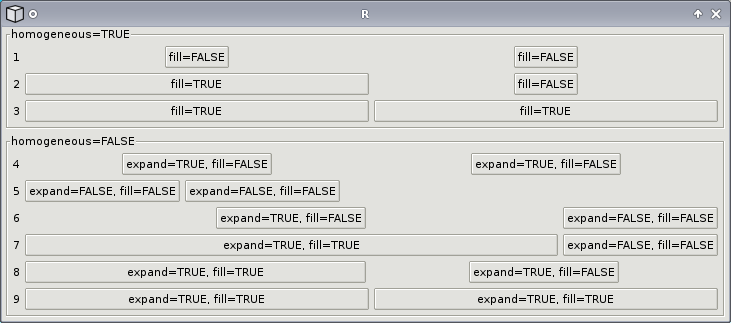
\includegraphics{packing.png}
    \caption{\label{fig:packing}A screenshot demonstrating the effect
      of packing two buttons into \class{GtkHBox} instances using the
      \method{packStart}{GtkBox} method with different combinations of
      the \argument{expand}{gtkBoxPackStart} and
      \argument{fill}{gtkBoxPackStart} settings.  The effect of the
      \argument{homogeneous}{gtkBoxPackStart} spacing setting on the
      \class{GtkHBox} is also shown.}
  \end{center}
\end{figure}

The code for some of these layouts is presented here. We begin by
creating a \class{GtkHBox} widget. We pass \code{TRUE} for the first
parameter, \argument{homogeneous}{gtkHBox}. This means that the
horizontal allocation of the box will be evenly distributed between
the children.  The second parameter directs the box to leave 5 pixels
of space between each child.  The following code constructs the
\class{GtkHBox}:
\begin{Schunk}
\begin{Sinput}
 box <- gtkHBox(TRUE, 5)
\end{Sinput}
\end{Schunk}
The equal distribution of available space is strictly enforced; the
minimum size requirement of a homogeneous box is set such that the box
always satisfies this assertion, as well as the minimum size
requirements of its children.

The \method{packStart}{GtkBox} and \method{packEnd}{GtkBox} methods pack a
widget into a box against the left and right side (top and
bottom for a \class{GtkVBox}), respectively. For this explanation, we
restrict ourselves to \method{packStart}{GtkBox}, since
\method{packEnd}{GtkBox} works the same except for the
direction. Below, we pack two buttons, \code{button\_a} and
\code{button\_b} against the left side:
\begin{Schunk}
\begin{Sinput}
 button_a <- gtkButton("Button A")
 button_b <- gtkButton("Button B")
 box$packStart(button_a, fill = FALSE)
 box$packStart(button_b, fill = FALSE)
\end{Sinput}
\end{Schunk}
%
First, \code{button\_a} is packed against the left side of the box,
and then we pack \code{button\_b} against the right side of
\code{button\_a}. This results in the first row in
Figure~\ref{fig:packing}. The space distribution is homogeneous, but
making the space available to a child does not mean that the child
will fill it. That depends on the natural size of the child, as well
as the value of the \argument{fill}{gtkBoxPackStart} parameter passed
to \method{packStart}{GtkBox}. In this case,
\argument{fill}{gtkBoxPackStart} is \code{FALSE}, so the extra space
is not filled and the widget is aligned in the center of its
space. When a widget is packed with the
\argument{fill}{gtkBoxPackStart} parameter set to \code{TRUE}, the
widget is resized to consume the available space. This results in
rows~$2$ and $3$ in Figure~\ref{fig:packing}.

In many cases, it is desirable to give children unequal amounts of
available space, as in rows~4--9 in Figure~\ref{fig:packing}. 
To create a heterogeneously spaced \class{GtkHBox}, we pass
\code{FALSE} as the first argument to the constructor, as in the
following code:
\begin{Schunk}
\begin{Sinput}
 box <- gtkHBox(FALSE, 5)
\end{Sinput}
\end{Schunk}

A heterogeneous layout is freed of the restriction that all widgets
must be given the same amount of available space; it only needs to
ensure that each child has enough space to meet its minimum size
requirement. After satisfying this constraint, a box is often left
with extra space. The programmer may control the distribution of this
extra space through the \argument{expand}{gtkBoxPackStart} parameter
to \method{packStart}{GtkBox}.  When a widget is packed with
\argument{expand}{gtkBoxPackStart} set to \code{TRUE}, we will call
the widget an \emph{expanding} widget. All expanding widgets in a box
are given an equal portion of the entirety of the extra space. If no
widgets in a box are expanding, as in row~5 of
Figure~\ref{fig:packing}, the extra space is left undistributed. 

It is common to mix expanding and non-expanding widgets in the same
box.
% FIXME: do we use the mirror dialog example or another one?  For
% example, in the CRAN mirrors dialog, the box first ensures that the
% mirror list and the label above it are given enough space to satisfy
% their minimum requirement. Then, since the mirror list is expanding,
% all of the extra space is made available to it, while the label is
% left only with its minimum requirement (i.e., enough space to show
% its text).
An example is given below, where \code{button\_a} is expanding,
while \code{button\_b} is not:
%
\begin{Schunk}
\begin{Sinput}
 box$packStart(button_a, expand = TRUE, fill = FALSE)
 box$packStart(button_b, expand = FALSE, fill = FALSE)
\end{Sinput}
\end{Schunk}
%
The result is shown in row~6 of Figure~\ref{fig:packing}.  The figure
contains several other permutations of the
\argument{homogeneous}{gtkBoxPackStart},
\argument{expand}{gtkBoxPackStart} and
\argument{fill}{gtkBoxPackStart} settings.

\begin{figure}
  \centering
  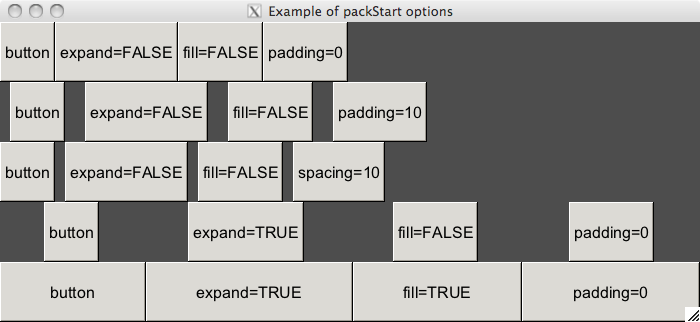
\includegraphics[width=.85\textwidth]{ex-RGtk2-pack-start}
  \caption{Examples of packing widgets into a box container. The top
    row shows no padding, whereas the 2nd and 3rd illustrate the
    difference between \code{padding} (an amount around each child)
    and \code{spacing} (an amount between each child). The last two
    rows show the effect of \code{fill} when \code{expand=TRUE}. This
    illustration follows one in original \GTK\/ tutorial.}
  \label{fig:RGtk2-pack-start}
\end{figure}

There are several ways to add space around widgets in a box container.
The \argument{spacing}{gtkHBox} argument for the constructors
specifies the amount of space, in pixels, between the cells. This
defaults to zero. The \code{pack} methods have a
\argument{padding}{gtkBoxPackStart} argument, also defaulting to zero,
for specifying the padding in pixels on either side of the child. It
is important to note the difference: \code{spacing} is between
children and the same for every boundary, while the \code{padding} is
specific to a particular child and occurs on either side, even on the
ends. The spacing between widgets is the sum of the \code{spacing}
value and the two \code{padding} values when the children are added.
Example~\ref{eg:RGtk2:mac-buttons} provides an example and
Figure~\ref{fig:RGtk2-pack-start} an illustration.

The \method{reorderChild}{gtkBox} method reorders the child
widgets. The new position of the child is specified using 0-based
indexing. This code will move the third child of \code{g} to the second position:
\begin{Schunk}
\begin{Sinput}
 b3 <- g[[3]]
 g$reorderChild(b3, 2 - 1)               # second is 2 - 1
\end{Sinput}
\end{Schunk}

\subsection{Alignment}
\label{sec:RGtk2:layout:align}

We began this section with a simple example of a window containing a
label:
\begin{Schunk}
\begin{Sinput}
 w <- gtkWindow(); w$setTitle("Hello world")
 l <- gtkLabel("Hello world")
 w$add(l)
\end{Sinput}
\end{Schunk}
%% again giving me issues
% <<basic-layout-align-window>>=
% <<basic-window-label>>
% @ 
%
The window allocates all of its space to the label, despite the actual
text consuming a much smaller region. The size of the text is fixed,
according to the font size, so it could not be expanded. Thus, the
label decided to center the text within itself (and thus the
window). A similar problem is faced by widgets displaying images. The
image cannot be expanded without distortion. Widgets that display
objects of fixed size inherit from \class{GtkMisc}, which provides
methods and properties for tweaking how the object is aligned within
the space of the widget. For example, the \code{xalign} and
\code{yalign} properties specify how the text is aligned in our label
and take values between $0$ and $1$, with $0$ being left and
top. Their defaults are $0.5$, for centered alignment. We modify them
below to make our label left justified:
\begin{Schunk}
\begin{Sinput}
 l["xalign"] <- 0
\end{Sinput}
\end{Schunk}

Unlike a block of text or an image, a widget usually does not have a
fixed size. However, the user may wish to tweak how a widget fills
the space allocated by its container.  \GTK\/ provides the
\class{GtkAlignment} container for this purpose. For example, rather
than adjust the justification of the label text, we could have
instructed the layout not to expand but to position itself against the
left side of the window:
\begin{Schunk}
\begin{Sinput}
 w <- gtkWindow(); w$setTitle("Hello world")
 a <- gtkAlignment()
 a$set(xalign = 0, yalign = 0.5, xscale = 0, yscale = 1)
 w$add(a)
 l <- gtkLabel("Hello world")
 a$add(l)
\end{Sinput}
\end{Schunk}

\section{Dialogs}
\label{sec:dialogs}

\GTK\/ provides a number of convenient dialogs for the common use
cases, as well as general infrastructure for constructing custom
dialogs.  A dialog is a window that generally consists of an icon, a
content area, and an action area containing a row of buttons
representing the possible user responses.  Typically, a dialog belongs
to a main application window and might be modal, in which case input
is blocked to other parts of the GUI.  \class{GtkDialog}
represents a generic dialog and serves as the base class for all
special purpose dialogs in \GTK.

\subsection{Message dialogs}
\label{sec:gtk-dialog-message}

Communicating textual messages to the user is perhaps the most common
application of a dialog. \GTK\/ provides the
\constructor{gtkMessageDialog} convenience wrapper for
\class{GtkDialog} for creating a message dialog showing a primary and
secondary message.  We construct one presently:
\begin{Schunk}
\begin{Sinput}
 w <- gtkWindow(); w['title'] <- "Parent window"
 #
 dlg <- gtkMessageDialog(parent=w, 
                         flags="destroy-with-parent",
                         type="question", 
                         buttons="ok",
                         "My message")
 dlg['secondary-text'] <- "A secondary message"
\end{Sinput}
\end{Schunk}
%

The \argument{flags}{gtkMessageDialog} argument allows one to specify
a combination of values from \code{GtkDialogFlags}. These include
\code{destroy-with-parent} and \code{modal}. Here, the dialog will be
destroyed upon destruction of the parent window. The
\argument{type}{gtkMessageDialog} argument specifies the message type,
using one of the $4$ values from \code{GtkMessageType}, which
determines the icon that is placed adjacent to the message text. The
\argument{buttons}{gtkMessageDialog} argument indicates the set of
response buttons with a value from \code{GtkButtonsType}. The
remaining arguments are pasted together into the primary message.  The
dialog has a \code{secondary-text} property that can be set to give a
secondary message.

Dialogs are optionally modal. Below, we enable modality by calling the
\method{run}{gtkDialog} method, which will additionally block the \R\/
session:
\begin{Schunk}
\begin{Sinput}
 response <- dlg$run()
 if(response == GtkResponseType["cancel"] || # for other buttons
    response == GtkResponseType["close"] ||
    response == GtkResponseType["delete-event"]) {
   ## pass
 } else if(response == GtkResponseType["ok"]) {
   print("Ok")
 }
\end{Sinput}
\begin{Soutput}
[1] "Ok"
\end{Soutput}
\begin{Sinput}
 dlg$Destroy()
\end{Sinput}
\end{Schunk}
%
The return value can then be inspected for the action, such as what
button was pressed. \class{GtkMessageDialog} will return response
codes from the \code{GtkResponseType} enumeration. We will see an
example of asynchronous response handling in the next section.

\subsection{Custom dialogs}
\label{sec:custom-dialogs}

The \constructor{gtkDialog} constructor returns a generic dialog
object which can be customized, in terms of its content and response
buttons.  Usually, a \class{GtkDialog} is constructed with
\constructor{gtkDialogNewWithButtons}, as a dialog almost always
contains a set of response buttons, such as \kbd{Ok}, \kbd{Yes},
\kbd{No} and \kbd{Cancel}.  In this example, we will create a simple
dialog showing a label and text entry:
\begin{Schunk}
\begin{Sinput}
 dlg <- gtkDialogNewWithButtons(title="Enter a value", 
                        parent=NULL, flags=0,
                        "gtk-ok", GtkResponseType["ok"],
                        "gtk-cancel", GtkResponseType["cancel"],
                        show=FALSE)
\end{Sinput}
\end{Schunk}
%
Buttons are added with a label and a response id, and their order is
taken from their order in the call. There is no automatic ordering
based on an operating system's conventions.  When the button label
matches a stock ID, the icon and text are taken from the stock
definition. We used standard responses from \code{GtkResponseType},
although in general the codes are simply integer values;
interpretation is up to the programmer.

The dialog has a content area, which is an instance of
\class{GtkVBox}. To complete our dialog, we place a labeled text entry
into the content area:
\begin{Schunk}
\begin{Sinput}
 hb <- gtkHBox()
 hb['spacing'] <- 10
 #
 hb$packStart(gtkLabel("Enter a value:"))
 entry <- gtkEntry()
 hb$packStart(entry)
 #
 vb <- dlg$getContentArea()
 vb$packStart(hb)
\end{Sinput}
\end{Schunk}
%
The content is placed above the button box, with a separator between them.

In the message dialog example, we called the \method{run}{GtkDialog}
method to make the dialog modal. To make a non-modal dialog, do not
call \method{run}{GtkDialog} but connect to the \code{response} signal
of the modal dialog. The response code of the clicked button is passed
to the callback:
\begin{Schunk}
\begin{Sinput}
 ID <- gSignalConnect(dlg, "response", 
                      f=function(dlg, resp, user.data) {
                        if(resp == GtkResponseType["ok"])
                          print(entry$getText()) # Replace this
                        dlg$Destroy()
                      })
 dlg$showAll()
 dlg$setModal(TRUE)
\end{Sinput}
\end{Schunk}

\subsection{File chooser}
\label{sec:RGtk2:file-chooser}

A common task in a GUI is the selection of files and directories, for
example to load or save a document. \class{GtkFileChooser} is an
interface shared by widgets that choose files. \GTK\/ provides three
such widgets. The first is \class{GtkFileChooserWidget}, which may be
placed anywhere in a GUI. The other two are based on the
first. \class{GtkFileChooserDialog} embeds the chooser widget in a
modal dialog, while \class{GtkFileChooserButton} is a button that
displays a file path and launches the dialog when clicked.

\begin{example}{An open file dialog}{ex:RGtk2:open-file}
  Here, we demonstrate the use of the dialog, the most commonly used
  of the three.  An open file dialog can be created with:
\begin{Schunk}
\begin{Sinput}
 dlg <- gtkFileChooserDialog(title="Open a file", 
                             parent=NULL, action="open",
                             "gtk-ok", GtkResponseType["ok"],
                             "gtk-cancel", GtkResponseType["cancel"],
                             show=FALSE)
\end{Sinput}
\end{Schunk}
  % 
  The dialog constructor allows one to specify a title, a parent and an
  action, either \code{open}, \code{save}, \code{select-folder} or
  \code{create-folder}. In addition, the dialog buttons must be
  specified, as with the last example using
  \code{gtkDialogNewWithButtons}.

  We connect to the \signal{response} signal
\begin{Schunk}
\begin{Sinput}
 gSignalConnect(dlg, "response", f=function(dlg, resp, data) {
   if(resp == GtkResponseType["ok"]) {
     filename <- dlg$getFilename()
     print(filename)
   }
   dlg$destroy()
 })
\end{Sinput}
\end{Schunk}
  % 
  The file selected is returned by
  \method{getFilename}{gtkFileChooser}. If multiple selection is enabled
  (via the \code{select-multiple} property) one should call the
  plural \method{getFilenames}{gtkFileChooser}.

  For the open dialog, one may wish to specify one or more filters that
  narrow the available files for selection:
\begin{Schunk}
\begin{Sinput}
 fileFilter <- gtkFileFilter()
 fileFilter$setName("R files")
 fileFilter$addPattern("*.R")
 fileFilter$addPattern("*.Rdata")
 dlg$addFilter(fileFilter)
\end{Sinput}
\end{Schunk}
  % 
  The \constructor{gtkFileFilter} function constructs a filter, which is
  given a name and a set of file name patterns, before being added to
  the file chooser. Filtering by mime type is also supported.

\end{example}

The save file dialog would be similar. The initial filename could be
specified with \method{setFilename}{gtkFileChooser}, or folder with
\method{setFolder}{gtkFileChooser}. The
\code{do-overwrite-confirmation} property controls whether the user is
prompted when attempting to overwrite an existing file.

Other features not discussed here, include embedding of preview and
other custom widgets, and specifying shortcut folders.

\subsection{Other choosers}

There are several other types of dialogs for making common types of
selections. These include \code{GtkCalendar} for picking dates,
\code{GtkColorSelectionDialog} for choosing colors, and
\code{GtkFontSelectionDialog} for fonts. These are very high-level
dialogs that are trivial to construct and manipulate, at a cost of
flexibility.

\subsection{Print dialog}

Rendering documents for printing is outside our scope; however, we
will mention that \class{GtkPrintOperation} can launch the native,
platform-specific print dialog for customizing a printing
operation. See Example~\ref{sec:gtk-printing-graphics} for an example
of printing R graphics using \pkg{cairoDevice}.


\section{Special-purpose Containers}
\label{sec:containers}

In Section~\ref{RGtk2:layout}, we presented \class{GtkBox} and
\class{GtkAlignment}, the two most useful layout containers in
\GTK. This section introduces some other important containers. These
include the merely decorative \class{GtkFrame}; the interactive
\class{GtkExpander}, \class{GtkPaned} and \class{GtkNotebook}; and the
grid-style layout container \class{GtkTable}. All of these widgets are
derived from \class{GtkContainer}, and so share many methods.

\subsection{Framed containers}
\label{sec:RGtk2:gtkFrame}

The \constructor{gtkFrame} function constructs a container that draws
a decorative, labeled frame around its single child:
\begin{Schunk}
\begin{Sinput}
 frame <- gtkFrame("Options")
 vbox <- gtkVBox()
 vbox$packStart(gtkCheckButton("Option 1"), FALSE)
 vbox$packStart(gtkCheckButton("Option 2"), FALSE)
 frame$add(vbox)
\end{Sinput}
\end{Schunk}
%
A frame is useful for visually segregating a set of conceptually
related widgets from the rest of the GUI. The type of decorative
shadow is stored in the \code{shadow-type} property.  The
\method{setLabelAlign}{gtkFrame} aligns the label relative to the
frame. This is to the left, by default.

\subsection{Expandable containers}
\label{sec:RGtk2:gtkExpander}

The \class{GtkExpander} widget provides a button that hides and shows
a single child upon demand. This is often an effective mechanism for
managing screen space. Expandable containers are constructed by
\function{gtkExpander}:
\begin{Schunk}
\begin{Sinput}
 expander <- gtkExpander("Advanced")
 expander$add(frame)
\end{Sinput}
\end{Schunk}
%
Use \function{gtkExpanderNewWithMnemonic} if a mnemonic is desired.
\code{expanded} property, which can be accessed with
\method{getExpanded}{gtkExpander} and
\method{setExpanded}{gtkExpander}, represents the visible state of the
widget.  When the \code{expanded} property changes, the
\signal{activate} signal is emitted.

\subsection{Notebooks}
\label{sec:RGtk2:gtkNotebook}

The \constructor{gtkNotebook} constructor creates a notebook
container, a widget that displays an array of buttons resembling
notebook tabs. Each tab corresponds to a widget, and when a tab is
selected, its widget is made visible, while the others are hidden. If
\class{GtkExpander} is like a check button, \class{GtkNotebook} is
like a radio button group. 

We create a notebook and add some pages:
\begin{Schunk}
\begin{Sinput}
 nb <- gtkNotebook()
 nb$appendPage(gtkLabel("Page 1"), gtkLabel("Tab 1"))
\end{Sinput}
\begin{Soutput}
[1] 0
\end{Soutput}
\begin{Sinput}
 nb$appendPage(gtkLabel("Page 2"), gtkLabel("Tab 2"))
\end{Sinput}
\begin{Soutput}
[1] 1
\end{Soutput}
\end{Schunk}
%
A page specification consists of a widget for the page and a widget
for the tab. Any type of widget is accepted, although a label is
typically used for the tab.  This allows for more complicated tabs,
such as a box container with a label and close icon.

The tabs can be positioned on any of the four sides of the notebook;
this depends on the \property{tab-pos}{gtkNotebook} property, with a value from
\code{GtkPositionType}: \qcode{left}, \qcode{right}, \qcode{top}, or
\qcode{bottom}. By default, the tabs are on top. We move the current ones to the
bottom:
\begin{Schunk}
\begin{Sinput}
 nb['tab-pos'] <- "bottom"
\end{Sinput}
\end{Schunk}

Methods and properties that affect pages expect the page index,
instead of the page widget. To map from the child widget to the page
number, use the method \method{pageNum}{gtkNotebook}.  The
\property{page}{gtkNotebook} property holds the zero-based index of the active
tab. We make the second tab active:
\begin{Schunk}
\begin{Sinput}
 nb['page'] <- 1
 nb['page']
\end{Sinput}
\begin{Soutput}
[1] 1
\end{Soutput}
\end{Schunk}
%
To move sequentially through the pages, calll the methods
\method{nextPage}{gtkNotebook} and
\method{prevPage}{gtkNotebook}. When the current page changes, the
\signal{switch-page} signal is emitted.

Pages can be reordered using the \method{reorderChild}{gtkNotebook},
although it is usually desirable to allow the user to reorder
pages. The \method{setTabReorderable}{GtkNotebook} enables drag and
drop reordering for a specific tab. It is also possible for the user
to drag and drop pages between notebooks, as long as they belong to
the same group, which depends on the \property{group-id}
property. Pages can be deleted using the method
\method{removePage}{gtkNotebook}.

\paragraph{Managing Many Pages}

By default, a notebook will request enough space to display all of its
tabs. If there are many tabs, space may be wasted. \class{GtkNotebook}
solves this with the scrolling idiom. If the
property \code{scrollable} is set to \code{TRUE}, arrows will be added
to allow the user to scroll through the tabs. In this case, the tabs
may become difficult to navigate. Setting the \code{enable-popup}
property to \code{TRUE} enables a right-click popup menu listing all
of the tabs for direct navigation.

\begin{example}{Adding a page with a close button}{eg:RGtk2-notebook-close-icon}
  A familiar element of notebooks in many web browsers is a tab close
  button. The following defines a new method
  \method{insertPageWithCloseButton}{gtkNotebook} that will use the
  themeable stock close icon.  The callback passes both the notebook
  and the page through the \code{data} argument, so that the proper
  page can be deleted.

\begin{Schunk}
\begin{Sinput}
 gtkNotebookInsertPageWithCloseButton <- 
   function(object, child, label.text="", position=-1) {
     label <- gtkHBox()
     label$packStart(gtkLabel(label.text))
     icon <- gtkImage(pixbuf = 
             object$renderIcon("gtk-close", "button", size="menu"))
     closeButton <- gtkButton()
     closeButton$setImage(icon)
     closeButton$setRelief("none")
     label$packEnd(closeButton)
     gSignalConnect(closeButton, "clicked", function(b) {
       index <- nb$pageNum(child)
       nb$removePage(index)
     })
     object$insertPage(child, label, position)
   }
\end{Sinput}
\end{Schunk}

Here is a simple demonstration of its usage:
\begin{Schunk}
\begin{Sinput}
 w <- gtkWindow()
 nb <- gtkNotebook(); w$add(nb)
 nb$insertPageWithCloseButton(gtkButton("hello"), 
                              label.text="page 1")
 nb$insertPageWithCloseButton(gtkButton("world"), 
                              label.text="page 2")
\end{Sinput}
\end{Schunk}
  
\end{example}


\subsection{Scrollable windows}
\label{sec:RGtk2:scroll-windows}

The \class{GtkExpander} and \class{GtkNotebook} widgets support
efficient use of screen real estate. However, when a widget is always
too large to fit in a GUI, partial display is necessary. A
\class{GtkScrolledWindow} supports this by providing scrollbars for
the user to adjust the visible region of a single child. The range,
step and position of \class{GtkScrollbar} are controlled by an
instance of \class{GtkAdjustment}, just as with the slider and spin
button. Scrolled windows are most often used with potentialy large
widgets like table views and when displaying images and graphics.

Our example will embed an R graphics device in a scrolled window and
allow the user to zoom in and out and pull on the scroll bars to pan
the view. First, we create an R graphics device using the
\pkg{cairoDevice} package
\begin{Schunk}
\begin{Sinput}
 library(cairoDevice)
 device <- gtkDrawingArea()
 device$setSizeRequest(600, 400)
 asCairoDevice(device)
\end{Sinput}
\begin{Soutput}
[1] TRUE
\end{Soutput}
\end{Schunk}
%
and then embed it within a scrolled window
\begin{Schunk}
\begin{Sinput}
 scrolled <- gtkScrolledWindow()
 scrolled$addWithViewport(device)
\end{Sinput}
\end{Schunk}
%
The widget in a scrolled window must know how to display only a part
of itself, i.e., it must be scrollable. Some widgets, including
\class{GtkTreeView} and \class{GtkTextView}, have native scrolling
support. Other widgets, like our \class{GtkDrawingArea}, must be
embedded within the proxy \class{GtkViewport}. The
\class{GtkScrolledWindow} convenience method
\method{addWithViewport}{GtkScrolledWindow} allows the programmer to
skip the \class{GtkViewport} step.


Next, we define a function for scaling the plot:
\begin{Schunk}
\begin{Sinput}
 zoomPlot <- function(x = 2.0) {
   allocation <- device$getAllocation()$allocation
   device$setSizeRequest(allocation$width * x, allocation$height * x)
   updateAdjustment <- function(adj) {
     adj$setValue(x * adj$getValue() + (x - 1) * adj$getPageSize() / 2)
   }
   updateAdjustment(scrolled$getHadjustment())
   updateAdjustment(scrolled$getVadjustment())
 }
\end{Sinput}
\end{Schunk}
%
The function gets the current size allocation from the device, scales
it by \qcode{x} and requests the new size. It then scrolls the window
to preserve the center point. The state of each scroll bar is
represented by a \class{GtkAdjustment}.  We will update the value of
the horizontal and vertical adjustments to scroll the window.  The
value of an adjustment corresponds to the left/top position of the
window, so we to adjust by half the page size after scaling the value.

We had key press events, so that pressing \kbd{+} zooms in and
pressing \kbd{-} zooms out:
\begin{Schunk}
\begin{Sinput}
 gSignalConnect(scrolled, "key-press-event", function(x, event) {
   key <- event[["keyval"]]
   if (key == GDK_plus)
     zoomPlot(2.0)
   else if (key == GDK_minus)
     zoomPlot(0.5)
   TRUE
 })
\end{Sinput}
\end{Schunk}

Despite its name, the scrolled window is not a top-level window. Thus,
it needs to be added to a top-level window:
\begin{Schunk}
\begin{Sinput}
 win <- gtkWindow(show = FALSE)
 win$add(scrolled)
 win$showAll()
\end{Sinput}
\end{Schunk}
 
Finally, a basic scatterplot is displayed in the viewer:
\begin{Schunk}
\begin{Sinput}
 plot(mpg ~ hp, data = mtcars)
\end{Sinput}
\end{Schunk}

The properties \code{hscrollbar-policy} and \code{vscrollbar-policy}
determine when the scrollbars are drawn. By default, they are always
drawn. The \qcode{automatic} value from the \code{GtkPolicyType}
enumeration draws the scrollbars only if needed, i.e, if the child
widget requests more space than can be allocated. The
\method{setPolicy}{gtkScrolledWindow} method allows both to be set at
once.

% \begin{example}{Scrolled window example}{eg:RGtk2:scrolled-window}
%   \SweaveInput{ex-RGtk2-scrolled-window}
% \end{example}

\subsection{Divided containers}
\label{sec:RGtk2:gtkPanedWindow}

The \constructor{gtkHPaned} and \constructor{gtkVPaned} constructors
create containers that contain two widgets, arranged horizontally or
vertically and separated by a handle.  The user may adjust the
position of the handle to apportion the allocation between the
widgets. We will demonstrate only the horizontal pane
\class{GtkHPaned} here, without loss of generality.
% An example is presented in Example \ref{eg:RGtk2:using-tree-content}. 

First, we construct an instance of \class{GtkHPaned}:
\begin{Schunk}
\begin{Sinput}
 paned <- gtkHPaned()
\end{Sinput}
\end{Schunk}

The two children may be added two different ways. The simplest
approach calls \method{add1}{gtkPaned} and
\method{add2}{gtkPaned} for adding the first and second child,
respectively. 
\begin{Schunk}
\begin{Sinput}
 paned$add1(gtkLabel("Left (1)"))
 paned$add2(gtkLabel("Right (2)"))
\end{Sinput}
\end{Schunk}
%
This configures the container such that both children are allowed to
shrink and only the second widget can expand. Such a configuration is
appropriate for a GUI with main widget and a side pane to the
left. More flexibility is afforded by the methods
\method{pack1}{gtkPaned} and \method{pack2}{gtkPaned}, which have
arguments for specifying whether the child should expand
(\qcode{resize}) and/or \qcode{shrink}. Here we add the children such
that both can expand and shrink:
\begin{Schunk}
\begin{Sinput}
 paned$pack1(gtkLabel("Left (1)"), resize = TRUE, shrink = TRUE)
 paned$pack2(gtkLabel("Right (2)"), resize = TRUE, shrink = TRUE)
\end{Sinput}
\end{Schunk}
%
After children are added, they can be retrieved from the container
through the \method{getChild1}{gtkPaned} and
\method{getChild2}{gtkPaned} methods.

The screen position of the handle can be set with the
\method{setPosition}{gtkPaned} method.  The properties
\code{min-position} and \code{max-position} are useful for converting
a percentage into a screen position. The \signal{move-handle} signal
is emitted when the gutter position is changed.

\subsection{Tabular layout}
\label{sec:RGtk2:gtkTable}

\class{GtkTable} is a container for laying out objects in a tabular
(or grid) format. It is \emph{not} meant for displaying tabular
data. The container divides its space into cells of a grid, and a
child widget may occupy one or more cells. The allocation of space
within a row or column follows logic similar to that of box
layouts. The most common use case of a \class{GtkTable} is form
layout, which we will demonstrate in our example.

\begin{example}{Dialog layout}{ex-RGtk2-dialog-layout}
This example shows how to layout a form in a dialog with some
attention paid to how the widgets are aligned and how they respond to
resizing of the window.

\begin{figure}
  \centering
  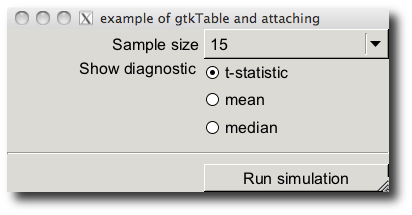
\includegraphics[width=.5\textwidth]{ex-RGtk2-dialog-layout}
  \caption{A basic dialog using a \code{gtkTable} container for layout.}
  \label{fig:RGtk2-dialog-layout}
\end{figure}

Our form layout will require $3$ rows and $2$ columns:
\begin{Schunk}
\begin{Sinput}
 tbl <- gtkTable(rows=3, columns=2, homogeneous=FALSE)
\end{Sinput}
\end{Schunk}
%
By default, the cells are allowed to have different sizes. This may be
overridden by passing \qcode{homogeneous = TRUE} to the constructor,
which forces all cells to have the same size.

We construct the widgets that will be placed in the form:
\begin{Schunk}
\begin{Sinput}
 sizeLabel <- gtkLabel("Sample size:")
 sizeCombo <- gtkComboBoxNewText()
 sapply(c(5, 10, 15, 30), sizeCombo$appendText)
 diagLabel <- gtkLabel("Diagnostic:")
 diagRadios <- gtkVBox()
 rb <- list()
 rb$t <- gtkRadioButton(label="t-statistic")
 rb$mean <- gtkRadioButton(rb, label="mean")
 rb$median <- gtkRadioButton(rb, label="median")
 sapply(rb, diagRadios$packStart)
 submitBox <- gtkVBox()
 submitBox$packEnd(gtkButton("Run simulation"), expand = FALSE)
\end{Sinput}
\end{Schunk}

The labels need to be aligned to the right, up against their
corresponding entry widgets, which should be left-aligned:
\begin{Schunk}
\begin{Sinput}
 sizeLabel['xalign'] <- 1
 diagLabel['xalign'] <- 1; diagLabel['yalign'] <- 0
 diagAlign <- gtkAlignment(xalign = 0)
 diagAlign$add(diagRadios)
\end{Sinput}
\end{Schunk}
% 
The labels are aligned through the \class{GtkMisc} functionality
inherited by \class{GtkLabel}. The \class{GtkVBox} with the radio
buttons does not support this, so we need to embed it within a
\class{GtkAlignment}. We have aligned the diagnostic label to the top
of its cell; otherwise, it would have been in the middle. The radio
buttons are left aligned, up against the label.

Child widgets are added to a table through the
\method{attach}{gtkTable} method.  The child can span more than one
cell. The arguments \argument{left.attach}{gtkTableAttach} and
\argument{right.attach}{gtkTableAttach} specify the horizontal bounds
of the child in terms of its left column and right column,
respectively. Analogously, \argument{top.attach}{gtkTableAttach} and
\argument{bottom.attach}{gtkTableAttach} define the vertical bounds.
By default, the widgets will expand into and fill the available space,
much as if \argument{expand}{gtkBoxPackStart} and
\argument{fill}{gtkBoxPackStart} were passed as \code{TRUE} to
\method{packStart}{GtkBox} (see
Section~\ref{sec:RGtk2:layout:box}). There is no padding between
children by default. Both the resizing behavior and padding may be
overridden by specifying additional arguments to
\method{attach}{GtkTable}.

The following attaches the combo box, radio buttons and their labels
to the table:
\begin{Schunk}
\begin{Sinput}
 tbl$attach(sizeLabel, left.attach=0,1, top.attach=0,1, 
            xoptions = c("expand", "fill"), yoptions="")
 tbl$attach(sizeCombo, left.attach=1,2, top.attach=0,1, 
            xoptions="fill", yoptions="")
 #
 tbl$attach(diagLabel, left.attach=0,1, top.attach=1,2, 
            xoptions = c("expand", "fill"), 
            yoptions=c("expand", "fill"))
 #
 tbl$attach(diagAlign, left.attach=1,2, top.attach=1,2, 
            xoptions=c("expand", "fill"), yoptions = "")
 #
 tbl$attach(submitBox, left.attach=1,2, top.attach=2,3, 
            xoptions="", yoptions=c("expand", "fill"))
\end{Sinput}
\end{Schunk}
%
The labels are allowed to expand and fill in the $x$ direction,
because correct alignment, to the right, requires them to have the
same size. The combo box is instructed to fill its space, as it would
otherwise be undesirably small, due to its short menu items. 

One can add spacing to the right of cells in a particular row or
column. Here we add $5$ pixels of space to the right of the label
column:
\begin{Schunk}
\begin{Sinput}
 tbl$setColSpacing(0, 5)
\end{Sinput}
\end{Schunk}

We complete the example by placing the table into a window:
\begin{Schunk}
\begin{Sinput}
 w <- gtkWindow(show=FALSE)
 w['border-width'] <- 14
 w$setTitle("GtkTable Example")
 w$add(tbl)
\end{Sinput}
\end{Schunk}

\end{example}


\chapter{RGtk2: Basic Components}
\label{sec:basic-components}


\section{Buttons}
\label{sec:RGtk2:gtkButton}

The button is the very essence of a GUI. It communicates its purpose
to the user and executes a command in response to a simple click or
key press. In \GTK\/, a basic button is usually constructed using
\constructor{gtkButton}, as the following example demonstrates.

\begin{example}{Button constructors}{eg:RGtk2:button-constructors}
\begin{Schunk}
\begin{Sinput}
 w <- gtkWindow(show=FALSE)
 w$setTitle("Various buttons")
 w$setDefaultSize(400, 25)
 g <- gtkHBox(homogeneous=FALSE, spacing=5)
 w$add(g)
 b <- gtkButtonNew() 
 b$setLabel("long way")
 g$packStart(b)
 g$packStart(gtkButton(label="label only") )
 g$packStart(gtkButton(stock.id="gtk-ok") )
 g$packStart(gtkButtonNewWithMnemonic("_Mnemonic") )
 w$show()
\end{Sinput}
\end{Schunk}
\end{example}

\begin{figure}
  \centering
  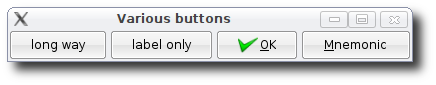
\includegraphics[width=.8\textwidth]{RGtk2-various-button}
  \caption{Various buttons}
  \label{fig:RGtk2:various-buttons}
\end{figure}

A \class{GtkButton} is simply a clickable region on the screen that is
rendered as a button. \class{GtkButton} is a subclass of
\class{GtkBin}, so it will accept any widget as an indicator of its
purpose. By far the most common button decoration is a label. The
first argument of \constructor{gtkButton},
\argument{label}{gtkButton}, accepts the text for an automatically
created \class{GtkLabel}. We have seen this usage in our ``Hello
World'' example and others.

Passing the \argument{stock.id}{gtkButton} argument to
\function{gtkButton} will use decorations associated with a so-called
stock identifier, see Section~\ref{sec:RGtk2:stock-icons}. For
example, ``gtk-ok'' would produce a button with a theme-dependent
image (such as a checkmark) and the ``Ok'' label, with the appropriate
mnemonic (see below) and language translation.  The available stock
identifiers are listed by \function{gtkStockListIds}.

The \constructor{gtkButtonNewWithMnemonic} constructor creates a
button with a mnemonic. A mnemonic is a key press that will activate
the button and is indicated by prefixing the character with an
underscore. In our example, we pass the string ``_Mnemonic'', so
pressing \kbd{Alt-M} will effectively press the button.

%% signals
\paragraph{Signals}

The \signal{clicked} signal is emitted when the button is clicked with
the mouse, when the associated mnemonic is pressed or when the button
has focus and the \kbd{enter} key is pressed. A callback can listen
for this event to perform a command when the button is clicked.

\begin{example}{Callback example for
    \code{gtkButton}}{eg:RGtk2:gtkButton-callback}

\begin{Schunk}
\begin{Sinput}
 w <- gtkWindow(); b <- gtkButton("click me");
 w$add(b)
 ID <- gSignalConnect(b,"button-press-event",   # just mouse
                      f = function(w,e,data) {
                        print(e$getButton())    # which button
                        return(FALSE)           # propagate
                      })
 ID <- gSignalConnect(b,"clicked",              # keyboard too
                      f = function(w,...) {
                        print("clicked")
                      })
\end{Sinput}
\end{Schunk}
\end{example}

As buttons are intended to call an action immediately after being
clicked, it is advisable to make them insensitive to user input when
the action is not possible. For example, we could set our button to be
insensitive: 
\begin{Schunk}
\begin{Sinput}
 b$setSensitive(FALSE)
\end{Sinput}
\end{Schunk}

%% Buttons initiate actions
Windows often have a default action. For example, if a window contains
a form, the default action submits the form. If a button
executes the default action for the window, the button can be
set so that it is activated when the user presses \kbd{enter} while
the parent window has the focus. To implement this, the property
\code{can-default} must be \code{TRUE} and the widget method
\method{grabDefault}{gtkWidget} must be called. (This is not specific
to buttons, but any widget that can be activatable.) The
\class{GtkDialog} widget and its derivatives facilitate the use of
buttons in this manner, see Section~\ref{sec:dialogs}.

If the action that a button initiates is to be represented elsewhere
in the GUI, say a menu bar, then a \code{GtkAction} object may be
appropriate. Action objects are covered in
Section~\ref{sec:RGtk2:UIManager}.

\begin{example}{Spacing between buttons}{eg:RGtk2:mac-buttons}
This example shows how to pack buttons into a box so that the spacing
between the similar buttons is 12 pixels, while potentially dangerous
buttons are separated from the rest by 24 pixels, as per the Mac human
interface guidelines.  

\GTK\/ provides the widget \class{GtkHButtonBox} for organizing
buttons in a manner consistent across an application. However, the
default layout modes would not yield the desired spacing. As such, we
will illustrate how to customize the spacing.  We assume that our
parent container, \code{hbox}, is a horizontal box container.


\begin{figure}
  \centering
  
\includegraphics[width=.85\textwidth]{ex-RGtk2-mac-buttons}
  \caption{Example using stock buttons with extra spacing added between the \code{delete} and \code{cancel} buttons.}
  \label{fig:ex-RGtk2-mac-buttons}
\end{figure}

We include standard buttons, so we use the stock names and icons.
\begin{Schunk}
\begin{Sinput}
 cancel <- gtkButton(stock.id="gtk-cancel")
 ok <- gtkButton(stock.id="gtk-ok")
 delete <- gtkButton(stock.id="gtk-delete")
\end{Sinput}
\end{Schunk}

We specify the padding as we pack the widgets into the box, from right
to left, with \method{packEnd}{GtkBox}:
\begin{Schunk}
\begin{Sinput}
 hbox$packEnd(ok, padding=0)
 hbox$packEnd(cancel, padding=12)
 hbox$packEnd(delete, padding=12)
 hbox$packEnd(gtkLabel(""), expand=TRUE, fill=TRUE)
\end{Sinput}
\end{Schunk}
%
The padding occurs to the left and right of the child.  The \code{ok}
button is given no padding. The \code{cancel} button is packed with 12
pixels of spacing, which separates it from the \code{ok}
button. Recognizing the \code{delete} button as potentially
irreversible, we add 12 pixels of separation between it and the
\code{cancel} button, for a total of 24 pixels. The blank label pushes
the buttons against the right side of the box.  We instruct the
\code{ok} button to grab focus, so that it becomes the default
button:
\begin{Schunk}
\begin{Sinput}
 ok$grabFocus()
\end{Sinput}
\end{Schunk}






\end{example}

\section{Static Text and Images}

\subsection{Labels}
\label{sec:RGtk2:gtkLabel}

The primary purpose of a label is to communicate the role of another
widget, as we showed for the button. Labels are created by the
\constructor{gtkLabel} constructor, which takes the label text as its
first argument. This text can be set with either
\method{setLabel}{gtkLabel} or \method{setText}{gtkLabel} and
retrieved with either \method{getLabel}{gtkLabel} or
\method{getText}{gtkLabel}.  The difference being the former
respects formatting marks.

\begin{example}{Label formatting}{eg:RGtk2:label-formatting}
  As most text in a \GTK\/ GUI is ultimately displayed by
  \class{GtkLabel}, there are many formatting options available.  This
  example demonstrates a sample of
  these~(Figure~\ref{fig:RGtk2:label-formatting})
  
  \begin{figure}
    \centering
    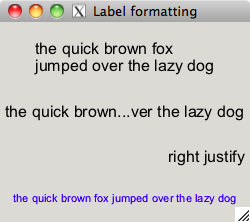
\includegraphics[width=.5\textwidth]{fig-RGtk2-labels}
    \caption{Various formatting for a label: wrapping, alignment,
      ellipsizing, PANGO markup}
    \label{fig:RGtk2:label-formatting}
  \end{figure}
  
\begin{Schunk}
\begin{Sinput}
 string <- "the quick brown fox jumped over the lazy dog"
 ## wrap by setting number of characters
 basicLabel <- gtkLabel(string)
 basicLabel$setLineWrap(TRUE)
 basicLabel$setWidthChars(35)            # no. characters
 ## Set ellipsis to shorten long text
 ellipsized <- gtkLabel(string)
 ellipsized$setEllipsize("middle")
 ## Right justify text lines
 ## use xalign property for aligning entire block
 rightJustified <- gtkLabel("right justify"); 
 rightJustified$setJustify("right")
 rightJustified['xalign'] <- 1
 ## PANGO markup
 pangoLabel <- gtkLabel()
 tmpl <- "<span foreground='blue' size='x-small'>%s</span>"
 pangoLabel$setMarkup(sprintf(tmpl, string))
 #
 sapply(list(basicLabel, ellipsized, rightJustified, pangoLabel), 
        g$packStart, expand = TRUE, fill = TRUE)
 w$showAll()
\end{Sinput}
\end{Schunk}
\end{example}

Many of the text formatting options are demonstrated in
Example~\ref{eg:RGtk2:label-formatting}. Line wrapping is enabled with
\method{setLineWrap}{gtkLabel}. Labels also support explicit line
breaks, specified with ``\code{\backslashn}.'' The
\method{setWidthChars}{gtkLabel} method is a convenience for instructing the
label to request enough space to show a specified number of
characters in a line.  When space is at a premium, long labels can be
ellipsized, i.e., have some of their text replaced with an
ellipsis, ``...''.  By default this is turned off; to enable, call
\method{setEllipsize}{gtkLabel}.  The property \code{justify}, with
values taken from \code{GtkJustification}, controls the alignment of
multiple lines within a label. To align the entire block of text
within the space allocated to the label, modify the \code{xalign}
property, as described in Section~\ref{sec:RGtk2:layout:align}.

\GTK\/ allows markup of text elements using the Pango text attribute
markup language, an XML-based format that resembles basic HTML. The
method \method{setMarkup}{gtkLabel} accepts text in the format. Text
is marked using tags to indicate the style. Some convenient tags are
\code{<b>} for bold, \code{<i>} for italics, \code{<ul>} for
underline, and \code{<tt>} for monospace text. Hyperlinks are possible
with \code{<a>}, as of version 2.18, and similar logic to
\function{browseURL} is implemented for launching a web
browser. Connect to the \signal{activate\_link} signal to
override it. More complicated markup involves the \code{<span>} tag
markup, such as \code{<span color='red'>some text</span>}. As with
HTML, the text may need to be escaped first so that designated
entities replace reserved characters.

Although mostly meant for static text display, \class{GtkLabel} has
some interactive features. If the \code{selectable} property is set to
\code{TRUE}, the text can be selected and copied into the clipboard.
Labels can hold mnemonics for other widgets; this is useful for
navigating forms. The mnemonic is specified at construction time with
\code{gtkLabelNewWithMnemonic}. The
\method{setMnemonicWidget}{gtkLabel} method identifies the widget to
which the mnemonic refers.

For efficiency reasons \class{GtkLabel} does not receive any input
events. It lacks an underlying \class{GdkWindow}, meaning that there
are no window system resources allocated for receiving the
events. Thus, to make a label interactive, one must first embed it
within a \class{GtkEventBox}, which provides the \class{GdkWindow}.

\subsection{Images}
\label{sec:RGtk2:images}

It is often said that a picture can be worth a thousand
words. Applying this to a GUI, images are often a more space efficient
alternative to labels. \class{GtkImage} is the widget that displays
images. The constructor \constructor{gtkImage} creates images from
various in-memory image representations, files, and other sources.
Images can be loaded after construction, as well. For example, the
\method{setFromFile}{gtkImage} method loads an image from a file.

\begin{example}{Using a pixmap to present graphs}{ex:RGtk2:pixbuf}





  This example shows how to use a \class{GtkImage} object to
  embed a graphic within \pkg{RGtk2}, using the
  \pkg{cairoDevice} package. The basic idea is to draw onto an
  off-screen pixmap using \pkg{cairoDevice} and
  then to construct a \class{GtkImage} from the pixmap. 

  We begin by creating a window of a certain size.
\begin{Schunk}
\begin{Sinput}
 w <- gtkWindow(show=FALSE); w$setTitle("Graphic window");
 w$setSizeRequest(400,400)
 hbox <- gtkHBox(); w$add(hbox)
 w$showAll()
\end{Sinput}
\end{Schunk}


The size of the image is taken as the size allocated to the box
\code{hbox}. This allows the window to be resized prior to drawing the
graphic. Unlike an interactive device, after drawing, this graphic
does not resize itself when the window resizes.
\begin{Schunk}
\begin{Sinput}
 theSize <- g$getAllocation()$allocation
 width <- theSize$width; height <- theSize$height
\end{Sinput}
\end{Schunk}

We create a \class{GdkPixmap} of the correct dimensions and
initialize an R graphics device that targets the pixmap. A simple
histogram is then plotted using base R graphics.
\begin{Schunk}
\begin{Sinput}
 require(cairoDevice)
 pixmap <- gdkPixmap(drawable = NULL, 
                     width = width, height = height, depth = 24)
 asCairoDevice(pixmap)
\end{Sinput}
\begin{Soutput}
[1] TRUE
\end{Soutput}
\begin{Sinput}
 hist(rnorm(100))
\end{Sinput}
\end{Schunk}

The final step is to create the \class{GtkImage} widget to display the
pixmap: 
\begin{Schunk}
\begin{Sinput}
 image <- gtkImage(pixmap = pixmap)
 hbox$packStart(image, expand=TRUE, fill = TRUE)
\end{Sinput}
\end{Schunk}

\end{example}


The image widget, like the label widget, does not have a parent
\class{GdkWindow}, which means it does not receive window events. As
with the label widget, the image widget can be placed inside a
\class{GtkEventBox} container if one wishes to connect to such
events.

\subsection{Stock icons}
\label{sec:RGtk2:stock-icons}

In \GTK\/, standard icons, like the one on the ``OK'' button, can be
customized by themes. This is implemented by a database that maps a
\textit{stock} identifier to an icon image. The stock identifier
corresponds to a commonly performed type of action, such as the ``OK''
response or the ``Save'' operation. There is no hard-coded set of
stock identifiers, however \GTK\/ provides a default set for the most
common operations. These identifiers are all prefixed with
``gtk-''. Users may register new types of stock icons.
%% ML: I believe there is an example of this in the RGtk2 demos

As mentioned previously, the full list of stock icons are returned in
a list by \function{gtkStockListIds}. The first $3$ are:
\begin{Schunk}
\begin{Sinput}
 head(unlist(gtkStockListIds()), n=3)   
\end{Sinput}
\begin{Soutput}
[1] "gtk-zoom-out" "gtk-zoom-in"  "gtk-zoom-fit"
\end{Soutput}
\end{Schunk}

The use of stock identifiers over specific images is encouraged, as it
allows an application to be customized through themes. The
\constructor{gtkButton} and \constructor{gtkImage} constructors accept
a stock identifier passed as \code{stock.id} argument, and the icons in
toolbars and menus are most conveniently specified by stock
identifier. 

% ML: Sorry, but I am not sure if this illustrates an important concept


% In the example below, we use the method \method{renderIcon}{gtkWidget} to
% return a pixbuf containing the icon that can be used with the
% constructor \constructor{gtkImageNewFromPixbuf} to display the
% icon. Here the stock id and size are specified to the
% \method{renderIcon}{gtkWidget} method.

% \begin{example}{\constructor{gtkButtonNewFromStock} -- the hard way}{ex:RGtk2:stock-icon}
% \SweaveInput{ex-RGtk2-button-new-stock-hardway}
% \end{example}

% ML: Could this example be in the book, but marked as optional or advanced?
%% JV Only for the package?? This will be placed in the package as an example.
% \begin{example}{Adding to the stock icons}{ex:RGtk2:add-stock-icons}
%   \SweaveInput{ex-RGtk2-add-stock-icon}
% \end{example}



%% Alertpanel application 
%% JV replaced this with one using reference Classes 
%% JV: This shows event boxes and reference classes, not a bad
%% thing but otherwise is just an info bar which isnow added. Should
%% we comment out?
%% ML: this is a fairly complicated example for a concept that is not
%% so important (GtkEventBox). I don't see how it's useful for
%% show/hide, which are pretty obvious.
%% JV: killed
% \begin{example}{An alert panel}{eg:RGtk2:alert-panel}
%   \SweaveInput{ex-RGtk2-alert-panel-2}
% \end{example}

\section{Input Controls}

\subsection{Text entry}
\label{sec:RGtk2:gtkEntry}

The widgets explained thus far are largely static. For example, \GTK\/
does not yet support editable labels. \GTK\/ has two different widgets
for editing text. One is optimized for multi-line text documents, the
other for single line entry. We will discuss complex multi-line text
editing in Section~\ref{sec:RGtk2:textviews}. For entering a single
line of text, the \class{GtkEntry} widget is appropriate:
\begin{Schunk}
\begin{Sinput}
 e <- gtkEntry()
\end{Sinput}
\end{Schunk}

The \code{text} property stores the text. This can be set with the
method \method{setText}{gtkEntry} and retrieved with
\method{getText}{gtkEntry}.  When the user has committed an entry,
e.g. by pressing the \kbd{enter} key, the \signal{activate} signal is
emitted. We connect to the signal and obtain the entered text upon
activation:
\begin{Schunk}
\begin{Sinput}
 gSignalConnect(e, "activate", function() {
   message("Text entered: ", e$getText())
 })
\end{Sinput}
\end{Schunk}

Sometimes the length of the text needs to be constrained to some
number of characters. The \argument{max}{gtkEntry} argument to
\function{gtkEntry} specifies this, but that usage is
deprecated. Instead, one should call \method{setMaxLength}{GtkEntry}.

\paragraph{The \class{GtkEditable} Interface}

Editing text programmatically relies on the \class{GtkEditable}
interface, which \class{GtkEntry} implements. The method
\method{insertText}{GtkEditable} inserts text before a position
specified by a $0$-based index. The return value is a list with the
component \code{position} indicating the position \textit{after} the
new text. The \method{deleteText}{GtkEditable} method deletes text
between two positions.

The example shows how to insert and then delete text:
\begin{Schunk}
\begin{Sinput}
 e$setText("Where did that guy go?")
 add.pos <- regexpr("guy", e['text']) - 1 # before "guy"
 ret <- e$insertText("@$#%! ", position = add.pos)
 e$getText()                             # or e['text']
\end{Sinput}
\begin{Soutput}
[1] "Where did that @$#%! guy go?"
\end{Soutput}
\begin{Sinput}
 e$deleteText(start = add.pos, end = ret$position)
 e$getText()
\end{Sinput}
\begin{Soutput}
[1] "Where did that guy go?"
\end{Soutput}
\end{Schunk}
% 

The \class{GtkEditable} interface supports three signals:
\signal{changed} when text is changed, \signal{delete-text} for delete
events, and \signal{insert-text} for insert events. It is possible to
prevent the insertion or deletion of text by connecting to the
corresponding signal and stopping the signal propagation with
\function{gSignalStopEmission}. 

\paragraph{Advanced \class{GtkEntry} Features}

\class{GtkEntry} has a number of features beyond basic text entry,
including: completion, buffer sharing, icons, and progress
reporting. We discuss completion in
Section~\ref{sec:RGtk2:entry-completion} and shared buffers in
Section~\ref{sec:RGtk2:buffer-sharing}. The progress reporting API,
introduced with version $2.16$, is virtually identical to that of
\class{GtkProgressBar}, introduced in
Section~\ref{sec:progress-bars}. We treat icons here. This feature has
been present since version $2.16$.

One can set an icon on an entry from a \class{GdkPixbuf}, stock ID,
icon name, or \class{GIcon}. Two icons are possible, one at the
beginning (\code{primary}) and one at the end (\code{secondary}). For
example, an entry might listen to its input and update its icon to
indicate whether the entered text is valid (in this case, consisting
only of letters):
%% JV: Cool, I didn't know this. The tooltip doesn't seem to work for
%% my setup.
\begin{Schunk}
\begin{Sinput}
 validatedEntry <- gtkEntry()
 gSignalConnect(validatedEntry, "changed", function(entry) {
   text <- entry$getText()
   if (nzchar(gsub("[a-zA-Z]", "", text))) {
     entry$setIconFromStock("primary", "gtk-no")
     validatedEntry$setIconTooltipText("primary", "Only letters are allowed")
   }
   else { 
     entry$setIconFromStock("primary", "gtk-yes")
     validatedEntry$setIconTooltipText("primary", NULL)
   }
 })
 validatedEntry$setIconFromStock("primary", "gtk-yes")
\end{Sinput}
\end{Schunk}
%
We add a tooltip on the error icon to indicate the nature of the
problem to the user. Icons can also be made clickable and used as a
source for drag and drop operations.

\subsection{Check button}
\label{sec:RGtk2:gtkCheckbox}

Very often, the action performed by a button simply changes the value
of a state variable in the application. \GTK\/ defines several types
of buttons that explicitly manage and display one aspect of the
application state. The simplest type of state variable is binary
(boolean/logical) and is usually proxied by a \class{GtkCheckButton}.

A \class{GtkCheckButton} is constructed by
\function{gtkCheckButton}:
\begin{Schunk}
\begin{Sinput}
 cb <- gtkCheckButton("Option")
\end{Sinput}
\end{Schunk}
%
The state of the binary variable is represented by the
\code{active} property. We check our button:
\begin{Schunk}
\begin{Sinput}
 cb['active']
\end{Sinput}
\begin{Soutput}
[1] FALSE
\end{Soutput}
\begin{Sinput}
 cb['active'] <- TRUE
\end{Sinput}
\end{Schunk}

When the state is changed the \signal{toggle} signal is emitted. The
callback should check the \code{active} property to determine if the
button has been enabled or disabled:
\begin{Schunk}
\begin{Sinput}
 gSignalConnect(cb, "toggled", function(x) {
   message("Button is ", if (x$active) "active" else "inactive")
 })
\end{Sinput}
\end{Schunk}

An alternative to \class{GtkCheckButton} is the lesser used
\class{GtkToggleButton}, which is actually the parent class of
\class{GtkCheckButton}. A toggle button is drawn as an ordinary
button. It remains depressed while the state variable is \code{TRUE},
instead of relying on a check box to communicate the binary value.

\subsection{Radio button groups}
\label{sec:RGtk2:gtkRadioButton}

\GTK\/ provides two widgets for discrete state variables that accept
more than two possible values: combo boxes, discussed in the next
section, and radio buttons. The \function{gtkRadioButton} constructor
creates an instance of \class{GtkRadioButton}, an extension of
\class{GtkCheckButton}. Each radio button belongs to a group and only
one button in a group may be active at once.

\begin{example}{Basic Radio Button Usage}{eg:gtk:radio-group-group-list} 
  When we construct a radio button, we need to add it to a
  group. There is no explicit group object; rather, the buttons are
  chained together as a linked list. By default, a newly constructed
  button is added to its own group. If the group list is passed to the
  constructor, the newly created button is added to the group:
\begin{Schunk}
\begin{Sinput}
 labels <- c("two.sided", "less", "greater")
 radiogp <- list()                                 # list for group
 radiogp[[labels[1]]] <- gtkRadioButton(label=labels[1]) # group = NULL
 for(label in labels[-1]) 
   radiogp[[label]] <- gtkRadioButton(radiogp, label=label)  # group is a list
\end{Sinput}
\end{Schunk}
%
As a convenience, there are constructor functions ending with
\code{FromWidget} that determine the group from a radio button
belonging to the group. As we will see in our second example, this
allows for a more natural \function{sapply} idiom that avoids the need
to allocate a list and populate it in a \code{for} loop.

We add each button to a vertical box:
\begin{Schunk}
\begin{Sinput}
 w <- gtkWindow(); w$setTitle("Radio group example")
 g <- gtkVBox(FALSE, 5); w$add(g)
 sapply(radiogp, gtkBoxPackStart, object = g)
\end{Sinput}
\end{Schunk}

We can set and query which button is active:
\begin{Schunk}
\begin{Sinput}
 g[[3]]$setActive(TRUE)           
 sapply(radiogp, `[`, "active") 
\end{Sinput}
\begin{Soutput}
two.sided      less   greater 
    FALSE     FALSE      TRUE 
\end{Soutput}
\end{Schunk}

The \code{toggle} signal is emitted when a button is toggled. We need
to connect a handler to each button:
\begin{Schunk}
\begin{Sinput}
 sapply(radiogp, gSignalConnect, "toggled",     # connect each
        f = function(w, data) {
          if(w['active']) # set before callback
            message("clicked", w$getLabel(),"\n")
        })
\end{Sinput}
\end{Schunk}
\end{example}

\begin{example}{Radio Group via a \function{FromWidget}
    Constructor}{eg:gtk:radio-group-get-group}
  In this example, we illustrate using the
  \constructor{gtkRadioButtonNewWithLabelFromWidget} function to add
  new buttons to the group:
\begin{Schunk}
\begin{Sinput}
 radiogp <- gtkRadioButton(label=labels[1])
 btns <- sapply(labels[-1], gtkRadioButtonNewWithLabelFromWidget, 
                group = radiogp)
 w <- gtkWindow()
 w['title'] <- "Radio group example"
 g <- gtkVBox(); w$add(g)
 sapply(rev(radiogp$getGroup()), gtkBoxPackStart, object = g)
\end{Sinput}
\end{Schunk}
%
The \method{getGroup}{gtkRadioButton} method returns a list containing
the radio buttons in the same group. However, it is in the reverse
order of construction (newest first). This results from an internal
optimization that prepends, rather than appends, the buttons to a
linked list. Thus, we need to call \function{rev} to reverse the list
before packing the widgets into the box.

\end{example}

\subsection{Combo boxes}
\label{sec:RGtk2:basic:combobox}

The combo box is a more space efficient alternative to radio buttons
and is better suited for when there are a large number of options. A
basic, text-only \class{GtkComboBox} is constructed by
\constructor{gtkComboBoxNewText}. In
Section~\ref{sec:RGtk2:mvc:combobox} we will discuss combo boxes that
are based on an external data model.

We construct and populate a simple combo box:
\begin{Schunk}
\begin{Sinput}
 combo <- gtkComboBoxNewText()
 sapply(c("two.sided", "less", "greater"), combo$appendText)
\end{Sinput}
\end{Schunk}
%

The index of the currently active item is stored in the
\property{active}{gtkComboBox} property. The index, as usual, is $0$-based,
and a value of $-1$ indicates that no value is selected:
\begin{Schunk}
\begin{Sinput}
 combo['active']
\end{Sinput}
\begin{Soutput}
[1] -1
\end{Soutput}
\end{Schunk}
%
The \method{getActiveText}{gtkComboBox} method retrieves
the text shown by the basic combo box.

When the active index changes, the \signal{changed} signal is
emitted. The handler then needs to retrieve the active index:
\begin{Schunk}
\begin{Sinput}
 gSignalConnect(combo, "changed",
                f = function(w, ...) {
                  if(w$getActive() < 0) 
                    cat("No value selected\n")
                  else
                    cat("Value is", w$getActiveText(), "\n")
                })
\end{Sinput}
\end{Schunk}

Although combo boxes are much more space efficient than radio buttons,
it can be difficult to use a combo box when there are a large number
of items. The \method{setWrapWidth}{gtkComboBox} method specifies
the preferred number of columns for displaying the items.

\begin{example}{Using one combo box to populate another}{ex:RGtk2-comboboxes}
%
The goal of this example is to populate a combo box of variables
whenever a data frame is selected in another. We use two convenience
functions from the \pkg{ProgGUIInR} package to find the possible data
frames, and for a data frame to find its variables.

We create the two combo boxes and the enclosing window:
\begin{Schunk}
\begin{Sinput}
 w <- gtkWindow(show=FALSE)
 w$setTitle("gtkComboBox example")
 df_combo <- gtkComboBoxNewText()
 var_combo <- gtkComboBoxNewText()
\end{Sinput}
\end{Schunk}
%

Our layout uses boxes. To add a twist, we will hide our variable combo box
until after a data frame has been initially selected.
\begin{Schunk}
\begin{Sinput}
 g <- gtkVBox(); w$add(g)
 #
 g1 <- gtkHBox(); g$packStart(g1)
 g1$packStart(gtkLabel("Data frames:"))
 g1$packStart(df_combo)
 #
 g2 <- gtkHBox(); g$packStart(g2)
 g2$packStart(gtkLabel("Variable:"))
 g2$packStart(var_combo)
 g2$hide()
\end{Sinput}
\end{Schunk}
%

Finally, we configure the combo boxes. When a data frame is selected, we
first clear out the variable combo box and then populate it:
\begin{Schunk}
\begin{Sinput}
 sapply(avail_dfs(), df_combo$appendText)
 df_combo$setActive(-1)
 #
 gSignalConnect(df_combo, "changed", function(w, ...) {
   var_combo$getModel()$clear()
   sapply(find_vars(w$getActiveText()),  var_combo$appendText)
   g2$show()
 })
\end{Sinput}
\end{Schunk}
%


\end{example}

An extension of \class{GtkComboBox}, \class{GtkComboBoxEntry},
replaces the main button with a text entry. This supports the entry of
arbitrary values, in addition to those present in the menu.

\subsection{Sliders}
\label{sec:RGtk2:sliders}

The slider widget and spin button widget allow selection from a
regularly spaced, semi-continuous list of values.
\class{GtkScale} implements a slider and may be oriented
either horizontally or vertically. This depends on the class:
\class{GtkHScale} or \class{GtkVScale}.  

\begin{example}{A slider controlling histogram bin selection}{ex:RGtk2:sliders}
  We demonstrate a slider for controlling the bin size of a
  histogram. First, we create and configure the horizontal slider:
\begin{Schunk}
\begin{Sinput}
 slider <- gtkHScale(min = 1, max = 100, step = 1)
 slider$setValue(10)
 slider['value-pos'] <- "bottom"
\end{Sinput}
\end{Schunk}
%
We specify the minimum, maximum and step values for the scale.  This
set of values is formally represented by the \class{GtkAdjustment}
structure, which could serve as a data model for synchronizing multiple
sliders or other scale-based widgets. Ordinarily, it is not necessary
to construct a \class{GtkAdjustment} explicitly. Instead, one passes
the values as parameters to the constructor. The initial value is set
to $10$, and the value will be rendered in a label beneath the slider,
according to the \property{value-pos}{GtkScale} property.

The \signal{value-changed} signal is emitted whenever the slider is
adjusted. Our handler updates the histogram:
\begin{Schunk}
\begin{Sinput}
 gSignalConnect(slider, "value-changed",
                f = function(w, ...) {
                  val <- w$getValue() 
                  drawHistogram(val)
                })
\end{Sinput}
\end{Schunk}

Finally, we load the data, define the \function{drawHistogram}
function, and finish the GUI:
\begin{Schunk}
\begin{Sinput}
 data <- rnorm(100)
 library(lattice)
 drawHistogram <- function(val) print(histogram(data, nint = val))
 drawHistogram(slider$getValue())        
 w <- gtkWindow(); w$setTitle("Histogram bin selection")
 w$add(slider)
\end{Sinput}
\end{Schunk}
\end{example}

%% properties
A few properties define the appearance of the slider widget.  The
\code{digits} property controls the number of digits after the decimal
point.  The property \code{draw-value} toggles the drawing of the
selected value near the slider. Finally, \code{value-pos},
demonstrated above, specifies where this value will be drawn using
values from \code{GtkPositionType}. The default is \code{top}.

\subsection{Spin buttons}
\label{sec:RGtk2:spinboxes}

The spin button widget is very similar to the slider widget,
conceptually and in terms of the \GTK\/ API. Spin buttons are
constructed with \constructor{gtkSpinButton}. As with sliders, this
constructor requires specifying adjustment values, either as a
\class{GtkAdjustment} or individually.  The methods
\method{getValue}{gtkSpinButton} and \method{setValue}{gtkSpinButton}
once again get and set the value. The \code{value-changed}
signal is emitted when the spin button value is changed.

\begin{example}{A range widget}{ex:RGtk2-range-widget}
This example shows how to make a range widget that combines both the
slider and spinbutton to choose a single number. Such a widget is
useful, as the slider is better at large changes and the spin button
better at finer changes. In \GTK\/ we use the same
\class{GtkAdjustment} model, so changes to one widget propagate
without effort to the other.


We name our scale parameters according to the corresponding arguments
to the \function{seq} function:
\begin{Schunk}
\begin{Sinput}
 from <- 0; to <- 100; by <- 1
\end{Sinput}
\end{Schunk}

The slider is drawn without a value, as the value is already displayed
by the spin button. The call to \constructor{gtkHScale} implicitly
creates an adjustment for the slider. The spin button is then created
with the same adjustment.
\begin{Schunk}
\begin{Sinput}
 slider <- gtkHScale(min=from, max=to, step=by)
 slider['draw-value'] <- FALSE
 adjustment <- slider$getAdjustment()
 spinbutton <- gtkSpinButton(adjustment = adjustment)
\end{Sinput}
\end{Schunk}
%
Our layout places the two widgets in a horizontal box container with
the slider, but not the spin button, set to expand into the available
space.
\begin{Schunk}
\begin{Sinput}
 g <- gtkHBox()
 g$packStart(slider, expand=TRUE, fill=TRUE, padding=5)
 g$packStart(spinbutton, expand=FALSE, padding=5)
\end{Sinput}
\end{Schunk}


\end{example}

A spin button has a few additional features. The property
\code{snap-to-ticks} can be set to \code{TRUE} to force the new value
to belong to the sequence of values in the adjustment. The \code{wrap}
property indicates whether the sequence will ``wrap'' around at the
bounds.

\section{Progress Reporting}

\subsection{Progress bars}
\label{sec:progress-bars}

It is common to use a progress bar to indicate the progress of a long
running computation. This implemented by \class{GtkProgressBar}. A
text label describes the current operation, and the progress bar
communicates the fraction completed:
\begin{Schunk}
\begin{Sinput}
 w <- gtkWindow(); w$setTitle("Progress bar example")
 pb <- gtkProgressBar()
 w$add(pb)
 #
 pb$setText("Please be patient...")
 for(i in 1:100) {
   pb$setFraction(i/100)
   Sys.sleep(0.05) ## replace with a step in the process
 }
 pb$setText("All done.")
\end{Sinput}
\end{Schunk}

Progress bars can also show indefinite activity by periodically
pulsing the bar: 
\begin{Schunk}
\begin{Sinput}
 pb$pulse()
\end{Sinput}
\end{Schunk}

\subsection{Spinners}

Related to a progress bar is the \class{GtkSpinner} widget, which is a
graphical heartbeat to assure the user that the application is still
alive during long-running operations. Spinners are commonly found in
web browsers. The basic usage is straightforward:
\begin{Schunk}
\begin{Sinput}
 spinner <- gtkSpinner()
 spinner$start()
 spinner$stop()
\end{Sinput}
\end{Schunk}


\section{Wizards}
\labe{sec:gtk-wizards}

The \class{GtkAssistant} class provides a wizard widget for \GTK. The
basic setup is one adds pages to the assistant object and they are
navigated in a linear manner. In our example, we will see how to
override this. 


Wizard pages have a certain type which must be declared. These are
enumerated in \code{GtkAssistantPageType} and set by \method{setPageType}{gtkAssistant}. The last page must be of
type \qcode{confirm}, \qcode{summary}, or \qcode{progress}.
Each wizard page has a content area and buttons.  As well, each page
in the assistant object has an optional side image, header image
and/or page title that may be customized. The buttons allow the user
to navigate through the wizard. The content area of a wizard page is
simply an instance of class \class{GtkWidget} (e.g., some container) and are
added to the assistant through the \method{appendPage}{gtkAssistant},
\method{insertPage}{gtkAssistant}, or
\method{prependPage}{gtkAssistant} methods. Pages are referred to by
the \class{GtkWidget} object or their page index, $0$-based. The
\code{forward} button on a page must be made sensitive by calling
\method{setPageComplete}{gtkAssistant} with the widget and logical
value.

%% signal
\paragraph{signals}
The \code{cancel} button emits a \signal{cancel} signal that can be
connected to for destroying the wizard widget. The \signal{apply}
signal is emitted on a page change. The \signal{prepare} signal is
emitted just before a page is made visible. This is needed to create
dynamically generated pages.

\begin{example}{An \code{install.packages} wizard}{eg-RGtk2-install-packages}

This example wraps the \function{install.packages} function into a
wizard with different pages for the (optional) selection of a CRAN
mirror, the selection of the package to install, the configuration
options provided and feedback. In general, wizards are quite common
for software installation.

We begin by defining our assistant and connecting to its
\signal{cancel} signal.
\begin{Schunk}
\begin{Sinput}
 asst <- gtkAssistant(show=FALSE)
 asst$setSizeRequest(500, 500)
 gSignalConnect(asst, "cancel", function(asst) asst$destroy())
\end{Sinput}
\end{Schunk}

Our pages will be computed dynamically. here we populate the pages
using box containers and specify their respective types. 
\begin{Schunk}
\begin{Sinput}
 pages <- lapply(1:5, gtkVBox, spacing=5, homogeneous=FALSE)
 page_types <- c("intro", rep("confirm",3), "summary")
 sapply(pages, gtkAssistantAppendPage, object=asst)
 sapply(pages, gtkAssistantSetPageType, object=asst, type=page_types)
\end{Sinput}
\end{Schunk}
%
We customize each page with a logo, using a side log here.
\begin{Schunk}
\begin{Sinput}
 image <- gdkPixbuf(filename = imagefile("rgtk-logo.gif"))[[1]]
 sapply(pages, gtkAssistantSetPageSideImage, object=asst, pixbuf=image)
\end{Sinput}
\end{Schunk}

When a page is about to be called we check and see if it has any
children, if not we call a function to create the page. These
functions are stored in a list so that they can be called by page index.
\begin{Schunk}
\begin{Sinput}
 populatePage <- list()                
 gSignalConnect(asst, "prepare", function(a, w, data) {
   page_no <- which(sapply(pages, identical, w))
   if(!length(w$getChildren()))
     populatePage[[page_no]]()
 })
\end{Sinput}
\end{Schunk}

Although we don't show how to create the CRAN selection page
(cf. Example~\ref{ex:RGtk2-add-toggle-to-df} for a similar
construction) we call \method{setForwardPageFunc}{gtkAssistant} to set
a function that will skip this page if it is not needed. This function
simply returns an integer with the next page number based on the last one.
\begin{Schunk}
\begin{Sinput}
 asst$setForwardPageFunc(function(i, data) {
   if(i == 0 && have_CRAN()) return(2L) else return(as.integer(i+1))
 }, data=NULL)
\end{Sinput}
\begin{Soutput}
NULL
\end{Soutput}
\end{Schunk}

We have a few script globals that allow us to pass data between pages.
\begin{Schunk}
\begin{Sinput}
 CRAN_package <- NA
 install_options <- list() #type, dependencies, lib
\end{Sinput}
\end{Schunk}






We now show how some of the pages are populated. The initial screen is
a welcome and simply shows a label. It is immediately complete.

\begin{Schunk}
\begin{Sinput}
 populatePage[[1]] <- function() {
   asst$setPageTitle(pages[[1]], "Install a CRAN package")
   pages[[1]]$packStart(l <- gtkLabel())
   pages[[1]]$packStart(gtkLabel(), expand=TRUE) # a spring
   
   l$setMarkup(paste("<span font='x-large'>Install a CRAN package</span>",
                     "This wizard will help install a package from <b>CRAN</b>",
                     "If you have not already specified a CRAN repository, one",
                     "you will be prompted to do so.",
                     sep="\n"))
   asst$setPageComplete(pages[[1]], TRUE)
 }
\end{Sinput}
\end{Schunk}


  
  

We skip showing the pages to select a CRAN site and a package, as they
are based on the forthcoming \class{GtkTreeView} class. On the
fourth page is a summary of the package taken from CRAN and a chance
for the user to configure a few options for \function{install.packages}.
\begin{Schunk}
\begin{Sinput}
 populatePage[[4]] <- function() {
   asst$setPageTitle(pages[[4]], "Install CRAN package")
   #
   get_desc <- function(pkgname) {
     x <- readLines(sprintf("http://cran.r-project.org/web/packages/%s/DESCRIPTION", pkgname))
     f <- tempfile(); cat(paste(x, collapse="\n"), file=f)
     read.dcf(f)
   }
   pkg_desc <- get_desc(CRAN_package)
   #
   l <- gtkLabel()
   l$setMarkup(paste(
                     sprintf("Install package: <b>%s</b>", pkg_desc[1, 'Package']),
                     "\n",
                     sprintf("%s", pkg_desc[1, 'Description']),
                     sep="\n"))
   
   pages[[4]]$packStart(l)
   #
   tbl <- gtkTable()
   pages[[4]]$packStart(tbl, expand=FALSE)
   pages[[4]]$packStart(gtkLabel(), expand=TRUE)
   
   #
   combo <- gtkComboBoxNewText()
   pkg_types <- c("source", "mac.binary", "mac.binary.leopard", "win.binary", "win64.binary")
   sapply(pkg_types, combo$appendText)
   combo$setActive(which(getOption("pkgType") == pkg_types) - 1)
   gSignalConnect(combo, "changed", function(w, ...) {
     install_options[['type']] <<- pkg_types[1 + w$getActive()]
   })
   tbl$attachDefaults(gtkLabel("Package type:"), 0, 1, 0, 1)
   tbl$attachDefaults(combo, 1, 2, 0, 1)
 
   #
   cb <- gtkCheckButton()
   cb$setActive(TRUE)
   gSignalConnect(cb, "toggled", function(w) {
     install_options[['dependencies']] <<- w$getActive()
   })
   tbl$attachDefaults(gtkLabel("Install dependencies"), 0, 1, 1, 2)
   tbl$attachDefaults(cb, 1, 2, 1, 2)
 
   #
   fc <- gtkFileChooserButton("Select a directory...", "select-folder")
   fc$setFilename(.libPaths()[1])
   gSignalConnect(fc, "selection-changed", function(w) {
     dir <- w$getFilename()
     install_options[['lib']] <<- dir
   })
   tbl$attachDefaults(gtkLabel("Where"), 0, 1, 2, 3)
   tbl$attachDefaults(fc, 1, 2, 2, 3)
 
   asst$setPageComplete(pages[[4]], TRUE)
 }
\end{Sinput}
\end{Schunk}

Our last page, where the selected package is installed, would
naturally be of type \code{progress}, but there is no means to
interrupt the flow of \function{install.packages} to update the
page. A real application would reimplement that. Instead we just set a
message once the package install attempt is done.
\begin{Schunk}
\begin{Sinput}
 populatePage[[5]] <- function() {
   asst$setPageTitle(pages[[5]], "Done")
   install_options$pkgs <- CRAN_package
   out <- try(do.call("install.packages", install_options), silent=TRUE)
 
   l <- gtkLabel(); pages[[5]]$packStart(l)
   if(!inherits(out, "try-error")) {
     l$setMarkup(sprintf("Package %s installed successfully", CRAN_package))
   } else {
     l$setMarkup(paste(sprintf("Package %s failed to install", CRAN_package),
                       paste(out, collapse="\n"),
                       sep="\n"))
   }
 
   asst$setPageComplete(pages[[5]], FALSE)
 }
\end{Sinput}
\end{Schunk}

To finish we simply need to populate the first page and call the
assistant's \meth{show} method.
\begin{Schunk}
\begin{Sinput}
 populatePage[[1]]()
 asst$show()
\end{Sinput}
\end{Schunk}
\end{example}

\section{Embedding R Graphics}
\label{sec:gtk-widget-graphics}

%% using cairoDevice to embed graphics
%% cairoDevice

The package \pkg{cairoDevice} is an R graphics device based on the
Cairo graphics library.  It supports alpha-blending and antialiasing
and reports user events through the \function{getGraphicsEvent}
function. \pkg{RGtk2} and \pkg{cairoDevice} are integrated through the
\function{asCairoDevice} function. If a \class{GtkDrawingArea},
\class{GdkDrawable}, \class{Cairo} context, or \class{GtkPrintContext}
is passed to \function{asCairoDevice}, an R graphics device will be
initialized that targets its drawing to the object. For simply
displaying graphics in a GUI, the \class{GtkDrawingArea} is the best
choice. 

This is the simplest usage:
\begin{Schunk}
\begin{Sinput}
 library(cairoDevice)
 device <- gtkDrawingArea()
 asCairoDevice(device)
\end{Sinput}
\begin{Soutput}
[1] TRUE
\end{Soutput}
\begin{Sinput}
 win <- gtkWindow(show=FALSE)
 win$add(device)
 win$showAll()
 plot(mpg ~ hp, data = mtcars)
\end{Sinput}
\end{Schunk}
%
We create the \class{GtkDrawingArea}, coerce it to a Cairo-based
graphics device, and place it in a window. Finally, we display a
scatterplot. Example~\ref{sec:RGtk2:scroll-windows} goes further by
embedding the drawing area into a scrolled window to support zooming
and panning.

For more complex use cases, such as compositing a layer above or below
the R graphic, one should pass an off-screen \class{GdkDrawable}, like
a \class{GdkPixmap}, or a \class{Cairo} context. The off-screen
drawing could then be composited with other images when
displayed. Example~\ref{ex:RGtk2:pixbuf} generates an icon by pointing
the device to a pixmap. Finally, passing a \class{GtkPrintContext} to
\function{asCairoDevice} allows printing R graphics through the \GTK\/
printing dialogs.

\begin{example}{Printing R Graphics}{eg:RGtk2:printing-graphics}
  This example will show how to use the printing support in \GTK\/ for
  printing an R plot. 
  
  A print operation is encapsulated by \class{GtkPrintOperation}:
\begin{Schunk}
\begin{Sinput}
 printOp <- gtkPrintOperation()
\end{Sinput}
\end{Schunk}
%
A print operation may perform several different actions: print
directly, print through a dialog, show a print preview and export to a
file. Before performing any such action, we need to implement the
rendering of our document into printed form. This is accomplished by
connecting to the \signal{draw-page} signal. The handler is passed a
\class{GtkPrintContext}, which contains the target Cairo context. In
general, one would call Cairo functions to render the document, which
is beyond our scope. In this case, though, we can pass the context
directly to \pkg{cairoDevice} for rendering the R plot:
\begin{Schunk}
\begin{Sinput}
 gSignalConnect(printOp, "draw-page", function(x, context, page_nr) {
   asCairoDevice(context)
   plot(mpg ~ wt, data = mtcars)
 })
\end{Sinput}
\end{Schunk}
%
  The final step is to run the operation to perform one of the
  available actions. In this example, we launch a print dialog:
\begin{Schunk}
\begin{Sinput}
 printOp$run(action = "print-dialog", parent = NULL)
\end{Sinput}
\end{Schunk}
% 
  When the user confirms the dialog, the
  \signal{draw-page} handler is invoked, and the
  rendered page is sent to the printer.
\end{example}

\section{Drag and drop}
\label{sec:RGtk2:dnd}

%% ------------ Drag and Drop

A drag and drop operation is the movement of data from a source widget
to a target widget. The source widget serializes the selected item as
MIME data, and the destination interprets that data to perform some
operation, often creating an item of its own. Our task is to configure
the source and destination widgets, so that they listen for the
appropriate events and understand each other. As a trivial example, we
allow the user to drag the text from one button to another.

\subsection{Initiating a Drag}

When a drag and drop is initiated, different types of data may be
transferred. We need to define a target type for each type of data, as
a \class{GtkTargetEntry} structure:
\begin{Schunk}
\begin{Sinput}
 TARGET.TYPE.TEXT   <- 80                 
 TARGET.TYPE.PIXMAP <- 81                  
 widgetTargetTypes <- 
   list(text = gtkTargetEntry("text/plain", 0, 
          TARGET.TYPE.TEXT),
        pixmap = gtkTargetEntry("image/x-pixmap", 0, 
          TARGET.TYPE.PIXMAP))
\end{Sinput}
\end{Schunk}
%
The first component of \class{GtkTargetEntry} is the name, which is often
a MIME type. The flags come next, which are usually left at $0$, and
finally we specify an arbitrary identifier for the target. We will
only use the \qcode{text} target in this example.

We construct a button and call \function{gtkDragSourceSet} to instruct
it to act as a drag source:
\begin{Schunk}
\begin{Sinput}
 w <- gtkWindow(); w['title'] <- "Drag Source"
 dragSourceWidget <-  gtkButton("Text to drag")
 w$add(dragSourceWidget)
 gtkDragSourceSet(dragSourceWidget,
        start.button.mask=c("button1-mask", "button3-mask"),
        targets=widgetTargetTypes[["text"]],
        actions="copy")
\end{Sinput}
\end{Schunk}
%
The \argument{start.button.mask}{gtkDragSourceSet}, with values from
\class{GdkModifierType}, indicates the modifier buttons that need to
be pressed to initiate the drag. The allowed target is \qcode{text} in
this case. The \argument{actions}{gtkDragSourceSet} argument lists the
supported actions, such as \code{copy} or \code{move}, from the
\class{GdkDragAction} enumeration.

When a drag is initiated, we will receive the \signal{drag-data-get}
signal, which needs to place some data into the passed
\class{GtkSelectionData} object:
\begin{Schunk}
\begin{Sinput}
 gSignalConnect(dragSourceWidget, "drag-data-get", 
                function(widget, context, sel, tType, eTime) {
                  sel$setText(widget$getLabel()) 
                })
\end{Sinput}
\end{Schunk}
%
If we had allowed the \code{move} action, we would also need to
connect to \signal{drag-data-delete}, in order to delete the data that
was moved away.

\subsection{Handling Drops}

In a separate window from the drag source button, we construct another
button and call \function{gtkDragDestSet} to mark it as a drag target:
\begin{Schunk}
\begin{Sinput}
 w <- gtkWindow(); w['title'] <- "Drop Target"
 dropTargetWidget <- gtkButton("Drop here")
 w$add(dropTargetWidget)
 gtkDragDestSet(dropTargetWidget,
                flags="all", 
                targets=widgetTargetTypes[["text"]],
                actions="copy")
\end{Sinput}
\end{Schunk}
%
The signature is similar to that of \function{gtkDragSourceSet},
except for the \argument{flags}{gtkDragDestSet} argument, which
indicates which operations, of the set \code{motion}, \code{highlight}
and \code{drop}, \GTK\/ will handle with reasonable default
behavior. Specifying \code{all} is the most convenient course, in
which case we only need to implement the extraction of the data from
the \class{GtkSelectionData} object. For a drop to occur, there must be a
non-empty intersection between the targets passed to
\function{gtkDragSourceSet} and those passed to
\function{gtkDragDestSet}.

When data is dropped, the destination widget emits the
\signal{drag-data-received} signal. The handler is responsible for
extracting the dragged data from \argument{selection} and performing some
operation with it. In this case, we set the text on the button:
\begin{Schunk}
\begin{Sinput}
 gSignalConnect(dropTargetWidget, "drag-data-received", 
        function(widget, context, x, y, sel, tType, eTime) {
          dropdata <- sel$getText()
          widget$setLabel(rawToChar(dropdata))
        })
\end{Sinput}
\end{Schunk}
%
The \argument{context} argument is a \class{GdkDragContext},
containing information about the drag event. The \argument{x} and
\argument{y} arguments are integer valued and represent the position
in the widget where the drop occurred. The text data is returned by
\function{getText} as a \code{raw} vector, so it is converted with
\function{rawToChar}.

%% JV: This could be expanded -- motion is not covered, as is done with
%% tcltk, but I don't think it is needed without a compelling use case.

%% ML: agreed

\chapter{RGtk2: Widgets Using Data Models}
\label{sec:RGtk2:widgets-with-models}

%% Possible outline:
%% - Displaying tabular data (GtkTreeView)
%%   - Loading data frame
%%   - Displaying data frame
%%   - Accessing GtkTreeModel (to set up selection, and hierarchical data)
%%   - Selection (an important concept, but common to hierarchical, below)
%%   - Sorting/filtering
%%   - Cell renderer details
%% - Displaying hierarchical data (GtkTreeView)
%%   - Loading hierarchical data
%%   - Displaying data as a tree
%% - Model-based combo boxes
%% - Text entry completion
%% - Icon views (currently omitted, probably OK)
%% - Text views

%% TODO: we need a unified example in the main text that spans loading
%% a data frame to sorting a model, at least.

Many widgets in \GTK\/ use the model, view, controller (MVC)
paradigm. For most, like the button, the MVC pattern is implicit;
however, widgets that primarily display data explicitly incorporate
the MVC pattern into their design. The data model is factored out as a
separate object, while the widget plays the role of the view and
controller. The MVC approach adds a layer of complexity but
facilitates the display of the dynamic data in multiple, coordinated
views.

\section{Display of tabular data}
\label{sec:RGtk2:tabular-heirarchical-data}

Widgets that display lists, tables and trees are all based on the same
basic data model, \class{GtkTreeModel}. Although its name suggests a
hierarchical structure, \class{GtkTreeModel} is also tabular. We first
describe the display of an \R\/ data frame in a list or table
view. The display of hierarchical data, as well as further details of
the \class{GtkTreeModel} framework, are treated subsequently.

\subsection{Loading a data frame}
\label{sec:tabular-stores-tree}

As an interface, \class{GtkTreeModel} may be implemented in any number
of ways. \GTK\/ provides simple in-memory implementations for
hierarchical and non-hierarchical data. For improved speed,
convenience and familiarity, \pkg{RGtk2} includes a custom
\class{GtkTreeModel} implementation called \class{RGtkDataFrame}, which
is based on an \R\/ data frame. For non-hierarchical data, this is
usually the model of choice, so we discuss it first.

\R\/ uses data frames to hold tabular data, where each column is of a
certain class, and each row is related to some observational
unit. This fits the structure of \class{GtkTreeModel} when there is no
hierarchy. As such it is natural to have a means to map a data frame
into a store for a tree view. \class{RGtkDataFrame} implements
\class{GtkTreeModel} to perform this role and is constructed with the
\constructor{rGtkDataFrame} function. Populating a
\class{RGtkDataFrame} is far faster than for a \GTK\/ model, because
data is retrieved from the data frame on demand. There is no need to
copy the data row by row into a separate data structure. Such an
approach would be especially slow if implemented as a loop in \R. The
constructor takes a data frame as an argument. The column classes are
important, so even if this data frame is empty, the user should
specify the desired column classes upon construction.

An object of class \class{RGtkDataFrame} supports the familiar S3
methods \method{[}{RGtkDataFrame}, \method{[\ASSIGN}{RGtkDataFrame},
\method{dim}{RGtkDataFrame}, and
\method{as.data.frame}{RGtkDataFrame}. The \code{[$<$-} method does
not have quite the same functionality as it does for a data
frame. Columns can not be removed by assigning values to \code{NULL},
and column types should not be changed. These limitations are inherit
in the design of \GTK: columns may not be removed from
\class{GtkTreeModel}, and views expect the data type to remain the
same.

\begin{example}{Defining and manipulating a \class{RGtkDataFrame}}{eg-RGtk2-manipulate-rGtkDataframe}
  The basic data frame methods are similar.
\begin{Schunk}
\begin{Sinput}
 data(Cars93, package="MASS")             # mix of classes
 model <- rGtkDataFrame(Cars93)
 model[1, 4] <- 12
 model[1, 4]                              # get value
\end{Sinput}
\begin{Soutput}
[1] 12
\end{Soutput}
\end{Schunk}
%
As with a data frame, assignment to a factor must be from one of the
possible levels.

\end{example}

The data frame combination functions \Rfunction{rbind} and
\Rfunction{cbind} are unsupported, as they would create a new data
model, rather than modify the model in place. Thus, one should add
rows with \method{appendRows}{rGtkDataFrame} and add columns with
\method{appendColumns}{rGtkDataFrame} (or sub-assignment, 
\method{[\ASSIGN}{RGtkDataFrame}).

The \method{setFrame}{rGtkDataFrame} method replaces the underlying
data frame.
\begin{Schunk}
\begin{Sinput}
 model$setFrame(Cars93[1:5, 1:5])
\end{Sinput}
\end{Schunk}
%
Replacing the data frame is the only way to remove rows, as this is
not possible with the conventional data frame sub-assignment
interface. Removing columns or changing their types remains
impossible. The new data frame cannot contain more columns and rows
than the current one. If the new data frame has more rows or columns,
then the appropriate \code{append} method should be used first.

\subsection{Displaying data as a list or table}
\label{sec:RGtk2:mvc:GtkTreeView}

%% intro
\class{GtkTreeView} is the primary view of \class{GtkTreeModel}.  It
serves as the list, table and tree widget in \GTK. A tree view is
essentially a container of columns, where every column has the same
number of rows. If the view has a single column, it is essentially a
list. If there are multiple columns, it is a table. If the rows are
nested, it is a tree table, where every node has values on the same
columns.

%% constructor
A tree view is constructed by \constructor{gtkTreeView}:
\begin{Schunk}
\begin{Sinput}
 view <- gtkTreeView(model)
\end{Sinput}
\end{Schunk}
Usually, as in the above, the model is passed to the
constructor. Otherwise, the model may be accessed with
\method{setModel}{gtkTreeView} and \method{getModel}{gtkTreeView}.

A newly created tree view displays zero columns, regardless of the
number of columns in the model. Each column, an instance of
\class{GtkTreeViewColumn}, must be constructed, inserted into the view and
instructed to render content based on one or more columns in the data
model:
\begin{Schunk}
\begin{Sinput}
 vc <- gtkTreeViewColumn()
 vc$setTitle("Manufacturer")
 cr <- gtkCellRendererText()
 vc$packStart(cr)
 vc$addAttribute(cr, "text", 0)
 view$insertColumn(vc, 0)
\end{Sinput}
\end{Schunk}
%
A column with the title ``Manufacturer'' is inserted at the first,
$0$-based, position. For displaying a simple data frame, we only need
to render text. Each row in a column consists of one or more cells,
managed in a layout. The number of cells and how each cell is rendered
is uniform down a column. As an implementation of
\class{GtkCellLayout}, \class{GtkTreeViewColumn} delegates the
responsibility of rendering to one or more \class{GtkCellRenderer}
objects. The cell renderers are packed into the column, which behaves
much like a box container. Rendering of text cells is the role of
\class{GtkCellRendererText}; we create an instance with
\constructor{gtkCellRendererText}. There are several properties that
control how the text is rendered. A so-called \textit{attribute} links
a model column to a renderer property. The most important property is
\code{text}, the text itself. In the example, we bind the \code{text}
property to the first ($0$-indexed) column in the model.

\class{GtkTreeView} provides the
\method{insertColumnWithAttributes}{gtkTreeView} convenience method to
perform all of these steps with a single call. We invoke it to add a
second column in our view:
\begin{Schunk}
\begin{Sinput}
 view$insertColumnWithAttributes(position = -1, 
      title = "Model", cell = gtkCellRendererText(), text = 1)
\end{Sinput}
\end{Schunk}
% 
The $-1$ passed as the first argument indicates that the column should
be appended. Next, we specify the column title, a cell renderer, and
an attribute that links the \code{text} renderer property to the
second column in the model. In general, any number of attributes may
be defined after the third argument.  We will use the above idiom in
all of the following examples, as it is much more concise than
performing each step separately.

To display the entire Cars93 data frame, we insert a view column for
every column in the data frame. Here, we reconstruct the view, inserting
a view column for every column in the data frame, i.e., the model.
\begin{Schunk}
\begin{Sinput}
 view <- gtkTreeView(model)
 mapply(view$insertColumnWithAttributes,  -1, colnames(model), 
        list(gtkCellRendererText()), 
        text = seq_len(ncol(model)) - 1)
\end{Sinput}
\end{Schunk}
%
Although it was relatively easy to create a \class{GtkTreeModel} for
the data frame using \class{RGtkDataFrame}, the complexity of
\class{GtkTreeView} complicates the task of displaying the data frame
in a simple, textual table. When this is all that is necessary, one
might consider \function{gtable} from \pkg{gWidgets}. For those
who wish to render text in each row differently (e.g., in a different
color) or fill cells with images, check boxes, progress bars and the
like, direct use of the \class{GtkTreeView} API is required.

\paragraph{Manipulating view columns}
The \class{GtkTreeView} widget is essentially a collection of
columns. Columns are added to the tree view with the methods
\method{insertColumn}{gtkTreeView} or, as shown above,
\method{insertColumnWithAttributes}{gtkTreeView}.  A column can be
moved with the \method{moveColumnAfter}{gtkTreeView} method, and
removed with the \method{removeColumn}{gtkTreeView} method. The
\method{getColumns}{gtkTreeView} method returns a list containing all
of the tree view columns.

There are several properties for controlling the behavior and
dimensions of a \class{GtkTreeViewColumn} instance. The property
\qcode{resizable} determines whether the user can resize a column, by
dragging with the mouse. The size properties \qcode{width},
\qcode{min-width}, and \qcode{fixed-width} control the size. The
visibility of the column can be adjusted through the
\method{setVisible}{gtkTreeViewColumn} method.

\paragraph{Additional Features}

Tree views have several special features, including sorting,
incremental search and drag-n-drop reordering. Sorting is discussed in
Section~\ref{sec:RGtk2:mvc:proxies}. To turn on searching,
\code{enable-search} should be \code{TRUE} (the default) and the
\code{search-column} property should be set to the column to be
searched. The tree view will popup a search box when the user types
\kbd{control-f}. To designate an arbitrary text entry widget as the
search box, call \method{setSearchEntry}{GtkTreeView}. The entry can
be placed anywhere in the GUI. Columns are always reorderable by drag
and drop. Reordering rows through drag-and-drop is enabled by the
\code{reorderable} property.

\paragraph{Aesthetic properties}

\class{GtkTreeView} is capable of rendering some visual guides. The
\code{rules-hint}, if \code{TRUE}, will instruct the theme to draw
rows in alternating colors. To show grid lines, set
\code{enable-grid-lines} to \code{TRUE}.

\subsection{Accessing \class{GtkTreeModel}}
\label{sec:RGtk2:mvc:iterators}

Although \class{RGtkDataFrame} provides a familiar interface for
manipulating the data in a \class{GtkTreeModel}, it is often necessary
to directly interact with the \GTK\/ API, such as when using another
type of data model or interpreting user selections. There are two
primary ways to index into the rows of a tree model: paths and
iterators.

To index directly into an arbitrary row, a \class{GtkTreePath} is
appropriate. For a table, a tree path is essentially the row number,
$0$-based; for a tree it is a sequence of integers referring to the
offspring index at each level. The sequence of integers may be
expressed as either a numeric vector or a string, using
\constructor{gtkTreePathNewFromIndices} or
\constructor{gtkTreePathNewFromString}, respectively. For a flat table
model, there is only one integer in the sequence:
\begin{Schunk}
\begin{Sinput}
 secondRow <- gtkTreePathNewFromIndices(2)
\end{Sinput}
\end{Schunk}
%
Referring to a row in a hierarchy is slightly more complex:
\begin{Schunk}
\begin{Sinput}
 abcPath <- gtkTreePathNewFromIndices(c(1, 3, 2))
 abcPath <- gtkTreePathNewFromString("1:3:2")
\end{Sinput}
\end{Schunk}
%
In the above, both paths refer to the second child of the third child
of the first top-level node. To recover the integer or string
representation of the path, use \method{getIndices}{GtkTreePath} or
\method{toString}{GtkTreePath}, respectively.

%% iters

The second means of row indexing is through an iterator,
\class{GtkTreeIter}, which is better suited for traversing a model.
While a tree path is an intuitive, transparent row index, an iterator
is an opaque index that is efficiently incremented. It is
probably most common for a model to be accessed in an iterative
manner, so all of the data accessor methods for \class{GtkTreeModel}
expect \class{GtkTreeIter}, not \class{GtkTreePath}. The \GTK\/
designers imagined that the typical user would obtain an iterator for
the first row and visit each row in sequence:
\begin{Schunk}
\begin{Sinput}
 iter <- model$getIterFirst()
 manufacturer <- character()
 while(iter$retval) {
   manufacturer <- c(manufacturer, model$get(iter$iter, 0)[[1]])
   iter$retval <- model$iterNext(iter$iter)
 }
\end{Sinput}
\end{Schunk}
%
In the above, we recover the manufacturer column from the Cars93 data
frame. Whenever a \class{GtkTreeIter} is returned by a
\class{GtkTreeModel}, the return value in \R\/ is a list of two
components: \code{retval}, a logical indicating whether the iterator
is valid, and \code{iter}, the pointer to the underlying C data
structure. The call to \method{get}{GtkTreeModel} also returns a list,
with an element for each column index passed as an argument. The
method \method{iterNext}{gtkTreeStore} updates the passed iterator in
place, i.e., by reference, to point to the next row. Thus, no new
iterator is returned. This is unfamiliar behavior in \R. Instead, the
method returns a logical value indicating whether the iterator is
still valid, i.e. \code{FALSE} is returned if no next row exists.

It is clear that the above usage is designed for languages like C,
where multiple return values are conveniently passed by reference
parameters. The iterator design also prevents the use of the apply
functions, which are generally preferred over the \code{while} loop
for reasons of performance and clarity. An improvement would be to
obtain the number of children, generate the sequence of row indices
and access the row for each index:
\begin{Schunk}
\begin{Sinput}
 nrows <- model$iterNChildren(NULL)
 manufacturer <- sapply(seq(nrows), function(i) {
   iter <- model$iterNthChild(NULL, i)
   model$get(iter$iter, 0)[[1]]
 })
\end{Sinput}
\end{Schunk}
%
Here we use \code{NULL} to refer to the virtual root node that sits
above the rows in our table. Unfortunately, this usage too is
unintuitive and slow, so the benefits of \class{RGtkDataFrame} should
be obvious.

One can convert between paths and iterators. The method
\method{getIter}{GtkTreeModel} on \class{GtkTreeModel} returns an
iterator for a path. A shortcut from the string representation of the
path to an iterator is \method{getIterFromString}{GtkTreeModel}. The
path pointed to by an iterator is returned by
\method{getPath}{GtkTreeModel}.

One final point: \class{GtkTreeIter} is created and managed by the
model, while \class{GtkTreePath} is model independent. It is not
possible to use iterators across models or even across modifications
to a model. After a model changes, an iterator is invalid. A tree path
may still point to a valid row, though it will not in general be the
same row from before the change. To refer to the same row across tree
model changes, use a \class{GtkTreeRowReference}.

\subsection{Selection}
%% selection: none, single browse multiple, getSelected

There are multiple modes of user interaction with a tree view: if the
cells are not editable, then selection is the primary mode.  A single
click selects the value, and a double click is often used to initiate
an action. If the cells are editable, then a double click or a click
on an already selected row will initiate editing of the
content. Editing of cell values is a complex topic and is handled by
derivatives of \class{GtkCellRenderer}, see
Section~\ref{sec:RGtk2:cellrenderers}. Here, we limit our discussion
to selection of rows.

\GTK\/ provides the class \class{GtkTreeSelection} to manage row
selection. Every tree view has a single instance of
\class{GtkTreeSelection}, returned by the
\method{getSelection}{gtkTreeView} method.

The usage of the selection object depends on the selection mode, i.e.,
whether multiple rows may be selected. The mode is configured with the
\method{setMode}{gtkTreeSelection} method, with values from
\code{GtkSelectionModel}, including \qcode{multiple} for allowing more
than one row to be selected and \qcode{single} for limiting selections
to a single row, or none. For example, we create a view and limit it
to single selection:
\begin{Schunk}
\begin{Sinput}
 model <- rGtkDataFrame(mtcars)
 view <- gtkTreeView(model)
 selection <- view$getSelection()
 selection$setMode("single")
\end{Sinput}
\end{Schunk}

When only a single selection is possible, the method
\method{getSelected}{gtkTreeSelection} returns the selected row as a
list, with components \code{retval} to indicate success, \code{model}
pointing to the tree model and \code{iter} representing an iterator to
the selected row in the model.
\begin{Schunk}
\begin{Soutput}
[1] 1
\end{Soutput}
\end{Schunk}
%
If our tree view is shown and a selection made, this code will
return the value in the first column:
\begin{Schunk}
\begin{Sinput}
 curSel <- selection$getSelected()
 with(curSel, model$getValue(iter, 0)$value)
\end{Sinput}
\begin{Soutput}
[1] 21.4
\end{Soutput}
\end{Schunk}
%
When multiple selection is permitted, then the method
\method{getSelectedRows}{gtkTreeSelection} returns a list with
the \code{model} and \code{retval}, a list
of tree paths.

To respond to a selection, connect to the \signal{changed} signal on
\class{GtkTreeSelection}. Upon a selection, this handler will print
the selected values in the first column:
\begin{Schunk}
\begin{Sinput}
 gSignalConnect(selection, "changed", function(selection) {
   curSel <- selection$getSelectedRows()
   if(length(curSel$retval)) {
     rows <- sapply(curSel$retval, gtkTreePathGetIndices) + 1L
     curSel$model[rows, 1]
   }
 })
\end{Sinput}
\end{Schunk}

%% double click
When a row is not editable, then the double-click event or a keyboard
command triggers the \signal{row-activated} signal for the tree
view. The callback has arguments \code{tree.view} pointing to the
widget that emits the signal, \code{path} storing a tree path of the
selected row, and \code{column} containing the tree view column. The
column number is not returned. If that is of interest, it can be
passed in via the user data argument, or matched against the children
of the tree view through a command like
\begin{Schunk}
\begin{Sinput}
 sapply(view$getColumns(), function(i) i == column)
\end{Sinput}
\end{Schunk}

\subsection{Sorting}
\label{sec:RGtk2:mvc:proxies}

A common GUI feature is sorting a table widget by column. By
convention, the user clicks on the column header to toggle
sorting. \class{GtkTreeView} supports this interaction, although the
actual sorting occurs in the model. Any model that implements the
\class{GtkTreeSortable} interface supports
sorting. \class{RGtkDataFrame} falls into this category. When
\class{GtkTreeView} is directly attached to a sortable model, it is
only necessary to inform each view column of the model column to use
for sorting when the header is clicked:
\begin{Schunk}
\begin{Sinput}
 vc <- view$getColumn(0)
 vc$setSortColumnId(0)
\end{Sinput}
\end{Schunk}
%
In the above, clicking on the header of the first view column,
\code{vc}, will sort by the first model column. Behind the scenes,
\class{GtkTreeViewColumn} will set its sort column as the sort column
on the model, i.e.:
\begin{Schunk}
\begin{Sinput}
 model$setSortColumnId(0, "ascending")
\end{Sinput}
\end{Schunk}

Some models, however, do not implement \class{GtkTreeSortable}, such
as \class{GtkTreeModelFilter}, introduced in the next section. Also,
sorting a model permanently changes the order of its rows, which may
be undesirable in some cases. The solution is to proxy the original
model with a sortable model. The proxy obtains all of its data from the
original model and reorders the rows according to the order of the
sort column. \GTK\/ provides \class{GtkTreeModelSort} for this:
\begin{Schunk}
\begin{Sinput}
 store <- rGtkDataFrame(mtcars)
 sorted <- gtkTreeModelSortNewWithModel(store)
 view <- gtkTreeView(sorted)
 view$insertColumnWithAttributes(0, "Click to sort", 
                                 gtkCellRendererText(), text=0)
 view$getColumn(0)$setSortColumnId(0)
\end{Sinput}
\end{Schunk}
%
When the user sorts the table, the underlying \code{store} will not be
modified. 

The default sorting function can be changed by calling the method
\method{setSortFunc}{gtkTreeSortable} on a sortable model.  The
following function shows how the default sorting might be implemented.
\begin{Schunk}
\begin{Sinput}
 f <- function(model, iter1, iter2, user.data) {
   column <- user.data
   val1 <- model$getValue(iter1, column)$value
   val2 <- model$getValue(iter2, column)$value
   as.integer(val1 - val2)
 }
 sorted$setSortFunc(sort.column.id=0, sort.func=f)
\end{Sinput}
\end{Schunk}


\subsection{Filtering}
\label{sec:RGtk2:mvc:filtering}

The previous section introduced the concept of a proxy model in
\class{GtkTreeModelSort}. Another common application of proxying is
filtering.  For filtering via a proxy model, \GTK\/ provides the
\class{GtkTreeModelFilter} class. The basic idea is that an extra
column in the base model stores logical values to indicate if a row
should be visible. The index of that column is passed to the filter
model, which provides only those rows where the filter column is
\code{TRUE}.

This is the basic usage:
\begin{Schunk}
\begin{Sinput}
 df <- data.frame(col=letters[1:3], vis=c(TRUE, TRUE, FALSE))
 store <- rGtkDataFrame(df)
 filtered <- store$filter()
 filtered$setVisibleColumn(1)            # 0-based
 view <- gtkTreeView(filtered)
\end{Sinput}
\end{Schunk}
%
The constructor of the filter model is \function{gtkTreeModelFilter},
which, somewhat coincidentally, also works as a method on the base
model, i.e., \code{model\$filter()}. To retrieve the original model
from the filter, call its \code{getModel} method. The method
\method{setVisibleColumn}{gtkTreeModelFilter} specifies which column
in the model holds the logical values.  To customize filtering, one
can register a function with \method{setVisibleFunc}. The callback,
given a row pointer, should return \code{TRUE} if the row passes the
filter, see Example~\ref{ex:RGtk2-variable-selection}. A filter model
may be treated as any other tree model, including attachment to a
\class{GtkTreeView}.


%% filter


\begin{example}{Using filtering}{ex:RGtk2-filtered}
This example shows how to use \class{GtkTreeModelFilter} to filter
rows according to whether they match a value entered into a text entry
box. The end result is similar to an entry widget with completion.


\begin{figure}
  \centering
  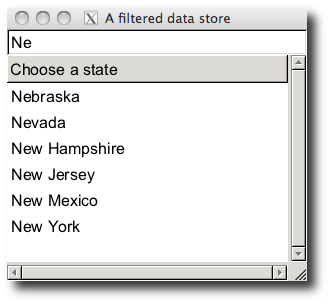
\includegraphics[width=.45\textwidth]{ex-RGtk2-filtered}
  \caption{Example of a data store filtered by values typed into a
    text-entry widget.}
  \label{fig:RGtk2-filtered}
\end{figure}

First, we create a data frame. The
\code{visible} column will be added to the \code{rGtkDataFrame}
instance to adjust the visible rows.
\begin{Schunk}
\begin{Sinput}
 df <- data.frame(state.name)
 df$visible <- rep(TRUE, nrow(df))
 store <- rGtkDataFrame(df)
\end{Sinput}
\end{Schunk}

The filtered store needs to have the column specified that contains
the logical values; in this example, it is the last column.
\begin{Schunk}
\begin{Sinput}
 filteredStore <- store$filter()
 filteredStore$setVisibleColumn(ncol(df)-1)      # offset
 view <- gtkTreeView(filteredStore)
\end{Sinput}
\end{Schunk}

Next, we create a basic view of a single column:
\begin{Schunk}
\begin{Sinput}
 view$insertColumnWithAttributes(0, "Col", 
                  gtkCellRendererText(), text = 0)
\end{Sinput}
\end{Schunk}

An entry widget will be used to control the filtering. In the
callback, we adjust the \code{visible} column of the
\code{rGtkDataFrame} instance to reflect the rows to be shown. When
\code{val} is an empty string, the result of \function{grepl} is 
\code{TRUE}, so all rows will be shown.
\begin{Schunk}
\begin{Sinput}
 e <- gtkEntry()
 gSignalConnect(e, "changed", function(w, data) {
   pattern <- w$getText()
   df <- data$getModel()
   values <- df[, "state.name"]
   df[, "visible"] <- grepl(pattern, values)
 }, data=filteredStore)
\end{Sinput}
\end{Schunk}


Figure~\ref{fig:RGtk2-filtered} shows the two widgets placed within a
simple GUI.
\end{example}

\subsection{Cell renderer details}
\label{sec:RGtk2:cellrenderers}

The values in a tree model are rendered in a rectangular cell by the
derivatives of \class{GtkCellRenderer}. Cell renderers are
interactive, in that they also manage editing and activation of cells.

A cell renderer is independent of any data model. Its rendering role
is limited to drawing into a specified rectangular region according to
its current property values. An object that implements the
\class{GtkCellLayout} interface, like \class{GtkTreeViewColumn} and
\class{GtkComboBox} (see Section~\ref{sec:RGtk2:mvc:combobox}),
associates a set of \emph{attributes} with a cell renderer. An
attribute is a link between an aesthetic property of a cell renderer
and a column in the data model. When the \class{GtkCellLayout} object
needs to render a particular cell, it configures the properties of the
renderer with the values from the current model row, according to the
attributes. Thus, the mapping from data to visualization depends on
the class of the renderer instance, its explicit property settings,
and the attributes associated with the renderer in the cell layout.

For example, to render text, a \class{GtkCellRendererText} is
appropriate. The \code{text} property is usually linked via an
attribute to a text column in the model, as the text would vary from
row to row. However, the background color (the \code{cell-background}
property) might be common to all rows in the column and thus is set
explicitly, without use of an attribute:
\begin{Schunk}
\begin{Sinput}
 renderer <- gtkCellRendererText()
 renderer['cell-background'] <- "gray"
\end{Sinput}
\end{Schunk}

The base class \class{GtkCellRenderer} defines a number of properties
that are common to all rendering tasks. The \code{xalign} and
\code{yalign} properties specify the alignment, i.e., how to position
the rendered region when it does not fill the entire cell. The
\code{cell-background} property indicates the color for the entire
cell background.

The rest of this section describes each type of cell renderer, as well
as some advanced features.

%% text/ numbers
\paragraph{Text cell renderers}

\constructor{GtkCellRendererText} displays text and numeric
values. Numeric values in the model are shown as strings.  The most
important property is \code{text}, the actual text that is
displayed. Other properties control the display of the text, such as
the font \code{family} and \code{size}, the \code{foreground} and
\code{background} colors, and whether to \code{ellipsize} or
\code{wrap} the text if there is not enough space for display. The
\code{wrap} attribute can be specified as \code{TRUE}, if the entries
are expected to be long. There are several other attributes that can
changed.  We display right-aligned text in a Helvetica font:
\begin{Schunk}
\begin{Sinput}
 cr <- gtkCellRendererText()
 cr['xalign'] <- 1                    # default 0.5 = centered
 cr['family'] <- "Helvetica"  
\end{Sinput}
\end{Schunk}

When an attribute links the \code{text} property to a numeric column
in the model, the property system automatically converts the number to
its string representation. This occurs according to the same logic
that \R\/ follows to print numeric values, so options like
\code{scipen} and \code{digits} are considered. See the ``Overriding
attribute mappings'' paragraph below for further customization.

%% perhaps could be adapted to demonstrate the above
% \begin{example}{A basic usage of displaying a data frame using a tree view}{ex:RGtk2-minimal-rGtkDataFrame}
%   \SweaveInput{ex-RGtk2-minimal-rGtkDataFrame}
% \end{example}

%% combo
\paragraph{Editable text renderers}

\class{GtkCellRendererCombo} and \class{GtkCellRendererSpin} allow
editing a text cell with a combo box or spin button,
respectively. Populating the combo box menu requires specifying two
properties: \code{model} and \code{text-column}. The menu items are
retrieved from the \class{GtkTreeModel} given by \code{model} at the
column index given by \code{text-column}.  If \code{has-entry} is
\code{TRUE}, a combo box entry is displayed.
\begin{Schunk}
\begin{Sinput}
 cr <- gtkCellRendererCombo()
 store <- rGtkDataFrame(state.name)
 cr['model'] <- store
 cr['text-column'] <- 0
 cr['editable'] <- TRUE                  # needed
\end{Sinput}
\end{Schunk}
%
The spin button editor is configured by setting a
\class{GtkAdjustment} on the \code{adjustment} property.


%% pixbuf
\paragraph{Pixbuf cell renderers}

To display an image in a cell, \class{GtkCellRendererPixbuf} is
appropriate. The image is specified through one of these properties:
\code{stock-id}, a stock identifier; \code{icon-name}, the name of a
themed icon; or \code{pixbuf}, an actual \code{GdkPixbuf} object,
holding an image in memory. Using a \class{list}, one can store a
\class{GdkPixbuf} in a \class{data.frame}, and thus an
\class{RGtkDataFrame}. This is demonstrated in the next example.

% <<rgtk2-mvc-pixbuf-in-df>>=
% library(RGtk2)
% apple <- gdkPixbuf(filename = imagefile("apple-red.png"))[[1]]
% floppy <- gdkPixbuf(filename = imagefile("floppybuddy.gif"))[[1]]
% logo <- gdkPixbuf(filename = imagefile("rgtk-logo.gif"))[[1]]
% rdf <- rGtkDataFrame(data.frame(image = I(list(apple, floppy, logo))))
% view <- gtkTreeView(rdf)
% view$insertColumnWithAttributes(0, "image", gtkCellRendererPixbuf(), pixbuf = 0)
% win <- gtkWindow()
% win$add(view)
% @


%% JV redid, a tighter programmed
\begin{example}{A variable selection widget}{ex:RGtk2-variable-selection}

%% ML: John, I changed this to explicitly treat the selected and
%% unselected widgets, instead of looping over the pairs. It just
%% seemed like looping over two discrete things added unnecessary
%% complexity. Sure, the code is a little more verbose now, but it's
%% probably more readable. The other big change was using one model
%% and a custom filter.

This example shows how to create a GUI for selecting variables from a
data frame. The GUI is based on two lists. The left one indicates the
variables that can be selected, and the right shows the variables that
have been selected. An icon, indicating the variable type, is placed
next to the variable name. A similar mechanism is part of the SPSS
model specification GUI of
Figure~\ref{fig:GUI:spss-11-term-selection}. For illustration purposes
we use the \code{Cars93} data set.
\begin{Schunk}
\begin{Sinput}
 df <- get(data(Cars93, package="MASS"))
\end{Sinput}
\end{Schunk}

First, we render an icon for each variable.  The \code{make\_icon}
function from the \pkg{ProgGUIinR} package creates an icon as a
\pkg{grid} object, which we render with \pkg{cairoDevice}:
% 
\begin{Schunk}
\begin{Sinput}
 make_icon_pixmap <- function(x, ...) {
   require(grid); require(cairoDevice)
   pixmap <- gdkPixmap(drawable=NULL, width=16, height=16, 
   depth=24)
   asCairoDevice(pixmap)
   grid.newpage()
   grid.draw(make_icon(x))
   dev.off()
   gdkPixbufGetFromDrawable(NULL, pixmap, NULL, 0,0,0,0,-1,-1)
 }
\end{Sinput}
\end{Schunk}

The two list views are based on the same underlying data model, which
contains three columns: the variable name, the icon, and
whether the variable has been selected. We construct the corresponding
data frame and wrap it in a \class{RGtkDataFrame}:
\begin{Schunk}
\begin{Sinput}
 mdf <- data.frame(Variables = I(sort(names(df))),
                   icon = I(sapply(df, make_icon_pixmap)),
                   selected = rep(FALSE, ncol(df)))
 model <- rGtkDataFrame(mdf)
\end{Sinput}
\end{Schunk}

The first view shows only unselected variables, while the other is
limited to selected variables. Thus, each view will be based on a
different filter:
\begin{Schunk}
\begin{Sinput}
 selectedFilter <- model$filter()
 selectedFilter$setVisibleColumn(2)
 unselectedFilter <- model$filter()
 unselectedFilter$setVisibleFunc(function(model, iter) {
   !model$get(iter, 2)[[1]]
 })
\end{Sinput}
\end{Schunk}
%
The selected filter is relatively easy to define, using
\code{selected} as the visible column. For the unselected filter, we
need to define a custom visible function that inverts the
\code{selected} column.

Next, we create a view for each filter:
\begin{Schunk}
\begin{Sinput}
 unselectedView <- gtkTreeView(unselectedFilter)
 selectedView <- gtkTreeView(selectedFilter)
 unselectedView$getSelection()$setMode('multiple')
 selectedView$getSelection()$setMode('multiple')
\end{Sinput}
\end{Schunk}

Each cell needs to display both an icon and a label.  This is achieved
by packing two cell renderers into the column:
\begin{Schunk}
\begin{Sinput}
 make_view_column <- function() {
   vc <- gtkTreeViewColumn()
   vc$setTitle("Variable")
   cr <- gtkCellRendererPixbuf()
   vc$packStart(cr)
   vc$addAttribute(cr, "pixbuf", 2)
   cr <- gtkCellRendererText()
   vc$packStart(cr)
   vc$addAttribute(cr, "text", 0)
   vc
 }
 unselectedView$insertColumn(make_view_column(), 0)
 selectedView$insertColumn(make_view_column(), 0)
\end{Sinput}
\end{Schunk}

For later use we extend the API for a tree view -- one method to find
the selected indices ($1$-based) and one to indicate if there is a
selection: 
\begin{Schunk}
\begin{Sinput}
 gtkTreeViewSelectedIndices <- function(object) {
   paths <- object$getSelection()$getSelectedRows()$retval
   out <- sapply(paths, function(i) {
     model <- object$getModel()          # Filtered!
     model$convertPathToChildPath(i)$toString()
   })
   if(length(out) == 0)
     integer(0)
   else
     as.numeric(out) + 1                             # 1-based
 }
 #
 gtkTreeViewHasSelection <- function(obj) length(obj$selectedIndices()) > 0
\end{Sinput}
\end{Schunk}

Now we create the buttons and connect to the \code{clicked}
signal. The handler moves the selected values to the other list by
toggling the \code{selected} variable:
\begin{Schunk}
\begin{Sinput}
 selectButton <- gtkButton(">")
 unselectButton <- gtkButton("<")
 toggleSelectionOnClick <- function(button, view) {
   gSignalConnect(button, "clicked", function (x) {
     ind <- view$selectedIndices()
     model[ind, "selected"] <- !model[ind, "selected"]
   })
 }
 toggleSelectionOnClick(selectButton, unselectedView)
 toggleSelectionOnClick(unselectButton, selectedView)
\end{Sinput}
\end{Schunk}
%
We only want our buttons sensitive if there is a possible move. This
is determined by the presence of a selection:
\begin{Schunk}
\begin{Sinput}
 selectButton['sensitive'] <- FALSE
 unselectButton['sensitive'] <- FALSE
 trackSelection <- function(button, view)
   gSignalConnect(view$getSelection(), "changed", 
                  function(x) button['sensitive'] <- view$hasSelection())
 trackSelection(selectButton, unselectedView)
 trackSelection(unselectButton, selectedView)
\end{Sinput}
\end{Schunk}

We now layout our GUI using a horizontal box, into which is packed the
views and a box holding the selection buttons. The views
will be scrollable, so we place them in scrolled windows:
\begin{Schunk}
\begin{Sinput}
 w <- gtkWindow(show=FALSE)
 w$setDefaultSize(600, 400)
 g <- gtkHBox()
 w$add(g)
 selectedScroll <- gtkScrolledWindow()
 selectedScroll$add(selectedView)
 selectedScroll$setPolicy("automatic", "automatic")
 unselectedScroll <- gtkScrolledWindow()
 unselectedScroll$add(unselectedView)
 unselectedScroll$setPolicy("automatic", "automatic")
 buttonBox <- gtkVBox()
 centeredBox <- gtkVBox()
 buttonBox$packStart(centeredBox, expand = TRUE, fill = FALSE)
 centeredBox$setSpacing(12)
 centeredBox$packStart(selectButton, expand = FALSE)
 centeredBox$packStart(unselectButton, expand = FALSE)
 g$packStart(unselectedScroll, expand=TRUE)
 g$packStart(buttonBox, expand=FALSE)
 g$packStart(selectedScroll, expand=TRUE)
\end{Sinput}
\end{Schunk}

Finally, we show the top-level window:
\begin{Schunk}
\begin{Sinput}
 w$show()
\end{Sinput}
\end{Schunk}


\end{example}

% %% ping pong
% \begin{example}{A widget for variable selection}{ex:RGtk2-pingpong}
%   \SweaveInput{ex-RGtk2-pingpong}
% \end{example}

\paragraph{Toggle cell renderers}

Binary data can be represented by a toggle. The
\constructor{gtkCellRendererToggle} will create a check box in the
cell that will appear checked if the \code{active} property is
\code{TRUE}. If an attribute is defined for the property, then changes
in the model will be reflected in the view. More work is required to
modify the model in response to user interaction with the view. The
\code{activatable} attribute for the cell must be \code{TRUE} in order
for it to receive user input. The programmer then needs to connect to the
\signal{toggled} to update the model in response to changes in the
active state.
\begin{Schunk}
\begin{Sinput}
 cr <- gtkCellRendererToggle()
 cr['activatable'] <- TRUE             # cell can be activated
 cr['active'] <- TRUE
 gSignalConnect(cr, "toggled", function(w, path) {
   model$active[as.numeric(path) + 1] <- w['active']
 })
\end{Sinput}
\end{Schunk}

To render the toggle as a radio button instead of a check box, set the
\code{radio} property to \code{TRUE}. Again, the programmer is
responsible for implementing the radio button logic via the
\code{toggled} signal.

\begin{example}{Displaying a check box column in a tree
    view}{ex:RGtk2-add-toggle-to-df}
This example demonstrates the construction of a GUI for selecting one
or more rows from a data frame. We will display a list of the installed
packages that can be upgraded from CRAN, although this code is
trivially generalizable to any list of choices. The user selects a row
by clicking on a 
check box produced by a toggle cell renderer.


To get the installed packages that can be upgraded, we use some of the
functions provided by the  \pkg{utils} package.
\begin{Schunk}
\begin{Sinput}
 d <- old.packages()[,c("Package", "Installed", "ReposVer")]
 d <- as.data.frame(d)
\end{Sinput}
\end{Schunk}


This function will be called on the selected rows. Here, we simply
call \function{install.packages} to update the selected packages.
\begin{Schunk}
\begin{Sinput}
 doUpdate <- function(d)  install.packages(d$Package)
\end{Sinput}
\end{Schunk}

To display the data frame, we first append a column to the data frame
to store the selection information and then create a corresponding
\class{RGtkDataFrame}.
\begin{Schunk}
\begin{Sinput}
 n <- ncol(d)
 nms <- colnames(d)
 d$.toggle <- rep(FALSE, nrow(d))
 store <- rGtkDataFrame(d)
\end{Sinput}
\end{Schunk}

Our tree view shows each text column using a simple text cell renderer,
except for the first column that contains the check boxes for selection.
\begin{Schunk}
\begin{Sinput}
 view <- gtkTreeView()
 # add toggle
 cr <- gtkCellRendererToggle()
 view$insertColumnWithAttributes(0, "", cr, active = n)
 cr['activatable'] <- TRUE
 gSignalConnect(cr, "toggled", function(cr, path, user.data) {
   view <- user.data
   row <- as.numeric(path) + 1
   model <- view$getModel()
   n <- dim(model)[2]
   model[row, n] <- !model[row, n]
 }, data=view)
\end{Sinput}
\end{Schunk}

The text columns are added in one go:
\begin{Schunk}
\begin{Sinput}
 mapply(view$insertColumnWithAttributes, -1, nms, 
        list(gtkCellRendererText()), text = 1:n-1)
\end{Sinput}
\end{Schunk}
%
Finally, we connect the store to the model.
\begin{Schunk}
\begin{Sinput}
 view$setModel(store)
\end{Sinput}
\end{Schunk}
%
To allow the user to initiate the action, we create a button and
assign a callback. We pass in the view, rather than the model, in case
the model would be recreated by the \code{doUpdate} call. In a real
application, once a package is upgraded it would be removed from the
display.
\begin{Schunk}
\begin{Sinput}
 b <- gtkButton("Update packages")
 gSignalConnect(b, "clicked", function(w, data) {
   view <- data
   model <- view$getModel()
   n <- dim(model)[2]
   vals <- model[model[, n], -n, drop=FALSE]
   doUpdate(vals)
 }, data=view)
\end{Sinput}
\end{Schunk}


Our basic GUI places the view into a box container that also holds the
button to initiate the action.
\begin{Schunk}
\begin{Sinput}
 w <- gtkWindow(show=FALSE)
 w$setTitle("Installed packages that need upgrading")
 w$setSizeRequest(300, 300)
 g <- gtkVBox(); w$add(g)
 sw <- gtkScrolledWindow()
 g$packStart(sw, expand=TRUE, fill=TRUE)
 sw$add(view)
 sw$setPolicy("automatic", "automatic")
 g$packStart(b, expand=FALSE)
 w$show()
\end{Sinput}
\end{Schunk}
\end{example}

%% progress bars
\paragraph{Rendering progress in cells}

To visually communicate progress within a cell, both progress bars and
spinner animations are supported. These modes correspond to
\class{GtkCellRendererProgress} and \class{GtkCellRendererSpinner},
respectively.

In the case of \class{GtkCellRendererProgress}, its \code{value}
property takes a value between $0$ and $100$ indicating the amount
finished, with a default value of $0$. Values out of this range will
be signaled by an error message.  For example,
\begin{Schunk}
\begin{Sinput}
 cr <- gtkCellRendererProgress()
 cr["value"] <- 50
\end{Sinput}
\end{Schunk}

For indicating progress in the absence of a definite end point,
\class{GtkCellRendererSpinner} is more appropriate. The spinner is
displayed when the \code{active} property is \code{TRUE}. Increment
the \code{pulse} property to drive the animation.

%% numbers
\paragraph{Overriding attribute mappings}

The default behavior for mapping model values to a renderer property
is simple: values are extracted from the model and passed directly to
the cell renderer property. If the data types are different, such as a
numeric value for a string property, the value is converted using
low-level routines defined by the property system. It is sometimes
desirable to override this mapping with more complex logic.

For example, conversion of numbers to strings is a non-trivial
task. Although the logic in the \R\/ print system often performs
acceptably, there is certainly room for customization. One example is
aligning floating point numbers by fixing the number of decimal
places. This could be done in the model (e.g., using
\function{sprintf} to format and coerce to character
data). Alternatively, one could preserve the integrity of the data and
perform the conversion during rendering. This requires intercepting
the model value before it is passed to the cell renderer. 

In the specific case \class{GtkTreeView}, it is possible to specify a
callback that overrides this step.  The callback, of type
\class{GtkTreeCellDataFunc}, is passed arguments for the tree view
column, the cell renderer, the model, an iterator pointing to the row
in the model and, optionally, an argument for user data. The function
is tasked with setting the appropriate attributes of the cell
renderer. For example, this callback would format floating point
numbers:
\begin{Schunk}
\begin{Sinput}
 func <- function(viewCol, cellRend, model, iter, data) {
   curVal <- model$getValue(iter, 0)$value
   fVal <- sprintf("%.3f", curVal)
   cellRend['text'] <- fVal
   cellRend['xalign'] <- 1
 }
\end{Sinput}
\end{Schunk}
%
The function then needs to be registered with a
\class{GtkTreeViewColumn} that is rendering a numeric column from the model:
\begin{Schunk}
\begin{Sinput}
 view <- gtkTreeView(rGtkDataFrame(data.frame(rnorm(100))))
 cr <- gtkCellRendererText()
 view$insertColumnWithAttributes(0, "numbers", cr, text = 0)
 vc <- view$getColumn(0)
 vc$setCellDataFunc(cr, func)
\end{Sinput}
\end{Schunk}
%
The last line is the key: calling
\method{setCellDataFunc}{GtkTreeViewColumn} registers our custom
formatting function with the view column.

One drawback with the use of such functions is that \R\/ code is
executed every time a cell is rendered. If performance matters,
consider pre-converting the data in the model or tweaking the
\code{options} in \R\/ for printing real numbers, namely \code{scipen}
and \code{digits}.

For customizing rendering further, and in the general case beyond
\class{GtkTreeView}, one could implement a new type of
\class{GtkCellRenderer}.  See Section~\ref{sec:gtk:extending-classes}
for more details on extending \GTK\/ classes.

%% This function will be set for the tree view column and illustrated in Example~\ref{ex:RGtk2:rGtk2DataFrame}.
%% editable cells 

\paragraph{Editable cells} When the \code{editable} property of a text
cell (or \code{activatable} property of a toggle cell) is set to
\code{TRUE}, then the cell contents can be changed. This allows the
user to make changes to the underlying model through the GUI. Although
the view automatically reflects changes made to the model, the reverse
is not true. A callback must be assigned to the \code{editable}
(\code{toggled}) signal for the cell renderer to implement the
change. The callback for the \qcode{edited} signal has arguments
\code{renderer}, \code{path} for the path of the selected row (as a
string), and \code{new.text} containing the value of the edited text
as a string. The tree view object and the column index are not passed
to the callback, unless one uses a closure or user data.
For example, here is how one can update an \code{RGtkDataFrame} model
from within the callback:
\begin{Schunk}
\begin{Sinput}
 cr['editable'] <- TRUE
 ID <- gSignalConnect(cr, "edited", 
 f=function(cr, path, newtext, user.data) {
   i <- as.numeric(path) + 1
   j <- user.data$column
   model <- user.data$model
   model[i, j] <- newtext
 }, data=list(model=store, column=1))
\end{Sinput}
\end{Schunk}
%
Before using editable cells to create a data frame editor, one should
see if the editor provided by the \function{gtkDfEdit} in the
\pkg{RGtk2Extras} package satisfies the requirements.

\paragraph{Moving the cursor}

Users may expect that once a cell is edited, the next cell is then set
up to be edited. In order to do this, one must advance the cursor and
activate editing of the next cell. For \class{GtkTreeView}, this is
implemented by the \method{setCursor}{gtkTreeView} method. The
\code{path} argument takes a tree path instance, the \code{column}
argument should be a tree view column object, and the flag
\code{start.editing} indicates whether to initiate editing.


\begin{example}{Using a table to gather arguments}{ex:RGtk2-options-in-table}

This example shows one way to gather arguments or options using an
editable cell in a table, rather than a separate text entry
widget. Tables can provide compact entry areas in a familiar
interface.

For this example we collect values for arguments to the
\function{title} function. We first create a data frame with the
argument name and default value, along with some additional values:
\begin{Schunk}
\begin{Sinput}
 opts <- c("main","sub","xlab","ylab", "line","outer")
 df <- data.frame(option=opts,
                  value=c("","","","","0","FALSE"),
                  class=c(rep("character", 4), "integer", "logical"),
                  edit_color=rep("gray95", 6),
                  dirty = rep(FALSE, 6),
                  stringsAsFactors=FALSE)
\end{Sinput}
\end{Schunk}
%
Unfortunately, we need to coerce the default values to character, in
order to store them in a single column. We preserve the class in the
\code{class} column, for coercion later. The \code{edit\_color} and
\code{dirty} columns are related to editing and explained later.
%

Now we create our model 
\begin{Schunk}
\begin{Sinput}
 m <- rGtkDataFrame(df)
 v <- gtkTreeView(m)
\end{Sinput}
\end{Schunk}
%
and configure the first column
\begin{Schunk}
\begin{Sinput}
 cr <- gtkCellRendererText()
 cr['background'] <- 'gray80'
 v$insertColumnWithAttributes(position=-1,
                              title="Option",
                              cell=cr,
                              text=1 - 1)
\end{Sinput}
\begin{Soutput}
[1] 1
\end{Soutput}
\end{Schunk}
%
The first column has a special background color which we specify
below, which indicates that the cells are not editable.
The second column is editable and has a background color that is
state dependent and indicates if a cell has been edited:
\begin{Schunk}
\begin{Sinput}
 cr <- gtkCellRendererText()
 cr['editable'] <- TRUE
 v$insertColumnWithAttributes(position = -1,
                              title = "Value",
                              cell = cr,
                              text = 2 - 1,
                              background = 4 - 1
                              )
\end{Sinput}
\end{Schunk}

To attach the view to the model, we connect the cell renderer to the
\signal{edited} signal. Here we use the \code{class} value to format
the text and then set the background color and \code{dirty} flag of the
entry. The latter allows one to easily find the values which were edited.
\begin{Schunk}
\begin{Sinput}
 gSignalConnect(cr, "edited", function(cr, path, new.text, 
                                       user.data) {
   m <- user.data$model
   i <- as.numeric(path) + 1; j <- user.data$column
   m[i,j] <- as(as(new.text, m[i, 'class']), "character")   # format
   m[i, 'dirty'] <- TRUE                                    # mark dirty
   m[i, 'edit_color'] <- 'gray70'                           # change color
 }, data=list(model=m, column=2))
\end{Sinput}
\end{Schunk}

A simple window displays our GUI.
\begin{Schunk}
\begin{Sinput}
 w <- gtkWindow(show=FALSE)
 w['title'] <- "Option editor"
 w$setSizeRequest(300,500)
 sw <- gtkScrolledWindow()
 w$add(sw)
 sw$add(v)
 w$show()
\end{Sinput}
\end{Schunk}

Implementing this into a GUI requires writing a function to map the
model values into the appropriate call to the \function{title} function. The
\code{dirty} flag makes this easy, but this is a task we do not pursue
here. Instead we add a bit of extra detail by providing a tooltip.

%% ML: This section makes me uncomfortable, since it's relying on very
%% volatile code. Internal routines from a package in active
%% development, which in turn rely on undocumented and internal
%% features of R.
\paragraph{Tooltips}
For this example, our function has built-in documentation. Below we
use the \pkg{helpr} function to extract the description for
each of the arguments. We leave this in a list, \code{descs}, for later
lookup.  
\begin{Schunk}
\begin{Sinput}
 require(helpr, quietly=TRUE)
 package <- "graphics"; topic <- "title"
 rd <- helpr:::parse_help(helpr:::pkg_topic(package, topic), 
                          package = package)
 descs <- rd$params$args
 names(descs) <- sapply(descs, function(i) i$param)
\end{Sinput}
\end{Schunk}

It is important to note that we are calling internal routines of a
package still under active development, which in turn relies on
volatile features of R. The purpose of this example is only to
demonstrate tooltips on a tree view.  For many widgets, adding a
tooltip is as easy as calling
\method{setTooltipText}{GtkWidget}. However, it is more complicated in
a tree view, as each cell should get a different tip.  To add tooltips
to the tree view we first indicate that we want tooltips, then connect
to the \signal{query-tooltip} signal to implement the tooltip:
\begin{Schunk}
\begin{Sinput}
 v["has-tooltip"] <- TRUE
 gSignalConnect(v, "query-tooltip", 
        function(w, x, y, key_mode, tooltip, user.data) {
          out <- w$getTooltipContext(x, y, key_mode)
          if(out$retval) {
            m <- w$getModel()
            i <- as.numeric(out$path$toString()) + 1
            val <- m[i, "option"]
            txt <- descs[[val]]$desc
            txt <- gsub("code>","b>", txt)  # no code in PANGO
            tooltip$setMarkup(txt)
            TRUE
          } else {
            FALSE                           # no tooltip
          }
        })
\end{Sinput}
\end{Schunk}
%
Within this callback we check if we have the appropriate context (we
are in a row), then, if so, use the path to find the description to
set in the tooltip. The descriptions use HTML for markup, but the
tooltip only uses PANGO. As the \code{code} tag is not PANGO, we
change to a bold tag using \function{gsub}.
\end{example}

%% XXX JV Add in an editable table example here, mention
%% RGtk2Extras:::gtkDfEdit

\section{Display of hierarchical data}
\label{sec:RGtk2:mvc:GtkTreeStore}

Although the \code{RGtkDataFrame} model is a convenient implementation
of \class{GtkTreeModel}, it has its limitations. Primary among them is
its lack of support for hierarchical data. \GTK\/ implements
\class{GtkTreeModel} with \class{GtkListStore} and
\class{GtkTreeStore}, which respectively store non-hierarchical and
hierarchical tabular data. \class{GtkListStore} is a flat table,
while \class{GtkTreeStore} organizes the table into a hierarchy. Here,
we discuss \class{GtkTreeStore}.

\subsection{Loading hierarchical data}
  
%% ML: I'm pretty sure that RGtkDataFrame will support the same types
%% of values as GtkListStore. It's just a little tricky to get a
%% column of GdkPixbuf externalptr's into a data.frame. Much easier to
%% use a character vector and associate it with the stock.id property
%% of GtkCellRendererPixbuf, as long as the images are registered icons.

%% construction
A tree store is constructed using \constructor{gtkTreeStore}. The
column types are specified through a character vector at the time of
construction. The specification uses ``GTypes'' such as
\code{gchararray} for character data, \code{gboolean} for logical
data, \code{gint} for integer data, \code{gdouble} for numeric data,
and \code{GObject} for \GTK\/ objects, such as pixbufs.

\begin{example}{Defining a tree}{eg:RGtk2:tree-store}
  Below, we create a tree based on the \code{Cars93} dataset, where
  the car models are organized by manufacturer, i.e., each model row
  is the child of its manufacturer row:
\begin{Schunk}
\begin{Sinput}
 tstore <- gtkTreeStore("gchararray")
 by(Cars93, Cars93$Manufacturer, function(df) {
   piter <- tstore$append()              # parent
   tstore$setValue(piter$iter, column = 0, value = df$Manufacturer[1])
   sapply(df$Model, function(model) {
     sibiter <- tstore$append(parent = piter$iter) # child
     if (is.null(sibiter$retval)) 
       tstore$setValue(sibiter$iter, column = 0, value = model)
   })
 })
\end{Sinput}
\end{Schunk}
  To retrieve a value from the tree store using its path we have:
\begin{Schunk}
\begin{Sinput}
 iter <- tstore$getIterFromString("0:0")
 tstore$getValue(iter$iter, column = 0)$value
\end{Sinput}
\begin{Soutput}
[1] "Integra"
\end{Soutput}
\end{Schunk}
This obtains the first model from the first manufacturer.

\end{example}

As shown in this example, populating a tree store relies on two
functions: \method{append}{GtkTreeStore}, for appending rows, and
\method{setValue}{GtkTreeStore}, for setting row values. The iterator
to the parent row is passed to \method{append}{GtkTreeStore}. A parent
of \code{NULL}, the default, indicates that the row should be at the
top level. It would also be possible to insert rows using
\method{insert}{GtkTreeStore}, \method{insertBefore}{GtkTreeStore}, or
\method{insertAfter}{GtkTreeStore}. The
\method{setValue}{GtkTreeStore} method expects the row iterator and
the column index, $0$-based.

An entire row can be assigned through the \method{set}{gtkTreeStore}
method. The method uses positional arguments to specify the column and
the value. The column index appears as an even argument (say $2k$) and
the corresponding value in the odd argument (say $2k+1$).  Values are
returned by the \method{getValue}{gtkListStore} method, in a list with
component \code{value} storing the value.

Traversing a tree store is most easily achieved through the use of
\class{GtkTreeIter}, introduced previously in the context of flat
tables. Here we perform a depth-first traversal of our \code{Cars93}
model to obtain the model values: 
\begin{Schunk}
\begin{Sinput}
 iter <- tstore$getIterFirst()
 models <- NULL
 while(iter$retval) {
   child <- tstore$iterChildren(iter$iter)
   while(child$retval) {
     models <- c(models, tstore$get(child$iter, 0)[[1]])
     child$retval <- tstore$iterNext(child$iter)
   }
   iter$retval <- tstore$iterNext(iter$iter)
 }
\end{Sinput}
\end{Schunk}
%
The hierarchical structure introduces the method
\method{iterChildren}{GtkTreeModel} for obtaining an iterator to the
first child of a row. As with other methods returning iterators, the
return value is a list, with the \code{retval} component indicating
the validity of the iterator, stored in the \code{iter} component. The
method \method{iterParent}{GtkTreeModel} performs the reverse,
iterating from child to parent.

\begin{figure}
  %% \centering
  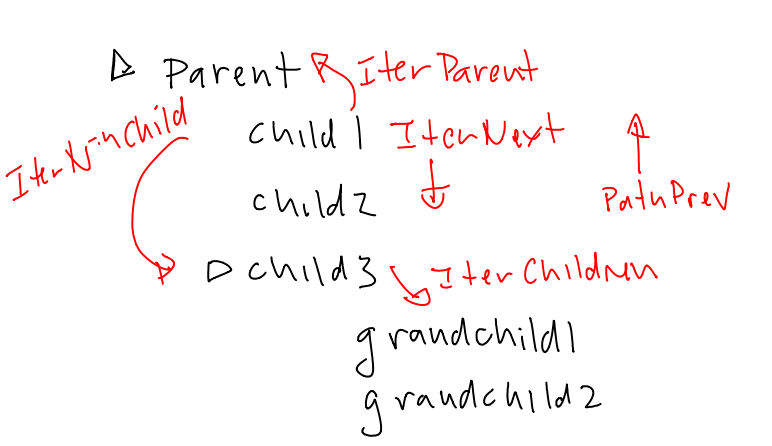
\includegraphics[width=.7\textwidth]{traverse-tree}
  \caption{[REPLACEME!] Graphical illustration of the functions used
    by iters to traverse a tree store. }
  \label{fig:traverse-iter}
\end{figure}

Rows within a store can be rearranged using several methods. Call
\method{swap}{gtkTreeStore} to swap rows referenced by their
iterators.  The methods \method{moveAfter}{gtkTreeStore} and
\method{moveBefore}{gtkTreeStore} move one row after or before
another, respectively.  The \method{reorder}{gtkTreeStore} method
totally reorders the rows under a specified parent given a vector of
row indices, like that returned by \function{order}.

%% clearing contents
Once added, rows may be removed using the
\method{remove}{gtkTreeStore} method. To remove every row, call the
\method{clear}{gtkTreeStore} method.

\subsection{Displaying data as a tree}
\label{sec:RGtk2:mvc:display-tree}

Once a hierarchical dataset has been loaded into a
\class{GtkTreeModel} implementation like \class{GtkTreeStore}, it can
be passed to a \class{GtkTreeView} widget for display as a
tree. Indeed, this is the same widget that displayed our flat data
frame in the previous section. As before, \class{GtkTreeView}
displays the \class{GtkTreeModel} as a table; however, it now adds
controls for expanding and collapsing nodes where rows are nested.

The user can click to expand or collapse a part of the tree. These
actions correspond to the signals \code{row-expanded} and
\code{row-collapsed}, respectively.

\begin{example}{A simple tree display}{eg:RGtk2-simple-tree}
Here, we demonstrate the application of \class{GtkTreeView} to the
display of hierarchical data. We will use the model constructed in
Example~\ref{eg:RGtk2:tree-store} from the \code{Cars93} dataset.  In
that example we defined a simple tree store from a data frame, with a
level for manufacturer and make for different cars. We refer to that
model by \code{tstore} below.



Now, we make a simple rectangular store for the model information with
the following:
\begin{Schunk}
\begin{Sinput}
 store <- rGtkDataFrame(Cars93[,"Model", drop=FALSE])
\end{Sinput}
\end{Schunk}

Creating a basic view is similar to that for rectangular data already presented:
\begin{Schunk}
\begin{Sinput}
 view <- gtkTreeView()
 view$insertColumnWithAttributes(0, "Make", 
            gtkCellRendererText(), text = 0)
\end{Sinput}
\begin{Soutput}
[1] 1
\end{Soutput}
\end{Schunk}


Finally, we illustrate that the same view can be used with either model:
\begin{Schunk}
\begin{Sinput}
 view$setModel(store)               # the rectangular store
 view$setModel(tstore)              # or the tree store
\end{Sinput}
\end{Schunk}
\end{example}

%% ## dynamic. 
%% JV: Is this too much? Perhaps leave for the package?
%% ML: Probably should move this to the package.
\begin{example}{Dynamically growing a tree}{eg:RGtk2:tree-dynamic}
This example uses a tree to explore an \R\/ list object, such as that
returned by one of \R's modeling functions.  As the depth of these
lists is not specified in advance, we use a dynamic approach to
that populates the tree store when a node is expanded and removes
nodes when their parent is collapsed.


We begin by defining our tree store and an accompanying tree
view. This example allows sorting, and so creates a sort proxy model:
\begin{Schunk}
\begin{Sinput}
 store <- gtkTreeStore(rep("gchararray", 2))
 sstore <- gtkTreeModelSort(store)
\end{Sinput}
\end{Schunk}

We create a root row:
\begin{Schunk}
\begin{Sinput}
 iter <- store$append(parent=NULL)$iter
 store$setValue(iter, column=0, "GlobalEnv")
 store$setValue(iter, column=1, "environment")
 iter <- store$append(parent=iter)
\end{Sinput}
\end{Schunk}
%
It is necessary to append an empty row to the root so that root
becomes expandable.

We now define the tree view and allow for multiple selection:
\begin{Schunk}
\begin{Sinput}
 view <- gtkTreeView(sstore)
 view$getSelection()$setMode("multiple")
\end{Sinput}
\end{Schunk}

The basic idea is to create child nodes when the parent is expanded
and to delete the children when the parent is collapsed. This relies
on the \code{row-expanded} and \code{row-collapsed} signals,
respectively. First, we define the expansion handler:
\begin{Schunk}
\begin{Sinput}
 gSignalConnect(view, signal = "row-expanded",
                f = function(view, iter, tpath, user.data) {
                  sortedModel <- view$getModel()
                  iter <- pathToIter(sortedModel, tpath)
                  path <- iterToRPath(sortedModel, iter)
                  children <- getChildren(path)
                  addChildren(store, children, parentIter=iter)
                  ## remove errant offspring, cf. addChildren
                  ci <- store$iterChildren(iter)
                  if(ci$retval) store$remove(ci$iter)
                })
\end{Sinput}
\end{Schunk}
%
The callback calls several helper functions to map the tree path to an
R object, get the child components of the object and add them to the
tree. The details are in the definitions of the helper functions.

The \function{pathToIter} function finds the iterator in the base tree
model for a tree path in the sorted proxy.
\begin{Schunk}
\begin{Sinput}
 pathToIter <- function(sstore, tpath) {
   store <- sstore$getModel()
   uspath <- sstore$convertPathToChildPath(tpath)
   store$getIter(uspath)$iter
 }
\end{Sinput}
\end{Schunk}

We now need to convert the iterator to an ``R path,'' which is made up
of the names of each component in the list. This function returns such
a path given an iterator:
\begin{Schunk}
\begin{Sinput}
 iterToRPath <- function(sstore, iter) {
   store <- sstore$getModel()
   indices <- store$getPath(iter)$getIndices()
   iter <- NULL
   path <- sapply(indices, function(i) {
     iter <<- store$iterNthChild(iter, i)$iter
     store$getValue(iter, 0)$value
   })
   return(path[-1])
 }
\end{Sinput}
\end{Schunk}

The \function{getChildren} function obtains the child components of a
given \R\/ object path. If the path is empty, the children are the
objects in the global environment, the root. The return value is a
\class{data.frame} with three columns: object name, object class and
whether the object is recursive.
\begin{Schunk}
\begin{Sinput}
 getChildren <- function(path=character(0)) {
   hasChildren <- function(obj) 
     (is.list(obj) || is.environment(obj)) && 
   !is.null(names(as.list(obj)))
   
   getType <- function(obj) head(class(obj), n=1)
 
   obj <- 
     if (!length(path)) {
       .GlobalEnv
     } else {
       x <- get(path[1], envir=.GlobalEnv)
       if(length(path) > 1)
         get(path[1], envir=.GlobalEnv)[[path[-1]]]
       else
         x
     }
 
   children <- as.list(obj)
   
   d <- data.frame(children = names(children),
                   class = sapply(children, getType),
                   offspring = sapply(children, hasChildren))
   
   ## filter out Gtk ones
   d[!grepl("^Gtk", d$class), ]
 }
\end{Sinput}
\end{Schunk}

The final step in the expansion handler is to add the children to the
tree store with the \function{addChildren} function.  Its one quirk is
the addition of a dummy child row when the item has children. This
makes the node expandable, i.e., the tree view draws an icon for the
user to click to request the expansion.
\begin{Schunk}
\begin{Sinput}
 addChildren <- function(store, children, parentIter = NULL) {
   if(nrow(children) == 0) 
     return(NULL)
   for(i in 1:nrow(children)) {
     iter <- store$append(parent=parentIter)$iter
     sapply(1:(ncol(children) - 1), function(j)              
            store$setValue(iter, column = j-1, children[i, j]))
     ## Add a branch if there are children
     if(children[i, "offspring"])
       store$append(parent=iter)
   }
 }
\end{Sinput}
\end{Schunk}

Next, we define a handler for the \code{row-collapsed} signal, which
has a similar signature as the \code{row-expanded} signal. The handler
removes the children of the newly collapsed node, so that we can add
them again when the node is expanded.
\begin{Schunk}
\begin{Sinput}
 gSignalConnect(view, signal = "row-collapsed",
        f = function(view, iter, tpath, user.data) {
          sortedModel <- view$getModel()
          iter <- pathToIter(sortedModel, tpath)
          n = store$iterNChildren(iter)
          if(n > 1) { ## n=1 gets removed when expanded
            for(i in 1:(n-1)) {
              child.iter <- store$iterChildren(iter)
              if(child.iter$retval)
                store$remove(child.iter$iter)
            }
          }
        })
\end{Sinput}
\end{Schunk}


Our last handler simply demonstrates the retrieval of an object when its
row is activated, i.e., double-clicked:
\begin{Schunk}
\begin{Sinput}
 gSignalConnect(view, signal = "row-activated",
        f = function(view, tpath, tcol) {
          sortedModel <- view$getModel()
          iter <- pathToIter(sortedModel, tpath)
          path <- iterToRPath(sortedModel, iter)
          sel <- view$getSelection()
          out <- sel$getSelectedRows()
          if(length(out) == 0) return(c()) # nothing
          vals <- c()
          for(i in out$retval) {  # multiple selections
            iter <- sortedModel$getIter(i)$iter
            newValue <- sortedModel$getValue(iter, 0)$value
            vals <- c(vals, newValue)
          }
          print(vals)  # [Replace this]
        })
\end{Sinput}
\end{Schunk}
 
To finish this example, we would need to populate the tree view with
columns and display the view in a window.



\end{example}
%% % ## mapes a list, shows how to update text view
% \SweaveInput{ex-RGtk2-tree-show}

\section{Model-based combo boxes}
\label{sec:RGtk2:mvc:combobox}

Basic combo box usage was discussed in
Section~\ref{sec:RGtk2:basic-combobox}; here we discuss the more
flexible and complex approach of using an explicit data model for
storing the menu items. The item data is tabular, although it is
limited to a single column. Thus, \class{GtkTreeModel} is again the
appropriate model, and \class{RGtkDataFrame} is usually the
implementation of choice.

To construct a \class{GtkComboBox} based on a user-created model, one
should pass the model to the constructor
\constructor{gtkComboBox}. This model may be changed or set through
the \method{setModel}{gtkComboBox} method and is returned by
\method{getModel}{gtkComboBox}. It remains to instruct the combo box
how to display one or more data columns in the menu. Like
\class{GtkTreeViewColumn}, \class{GtkComboBox} implements the
\class{GtkCellLayout} interface and thus delegates the rendering of
model values to \class{GtkCellRenderer} instances that are packed into
the combo box.

The \method{getActiveIter}{gtkComboBox} returns a list containing the iterator
pointing to the currently selected row in the model.  If no row has been
selected, the \code{retval} component of the list is \code{FALSE}.
The \method{setActiveIter}{gtkComboBox} sets the currently selected
item by iterator. As discussed previously, the
\method{getActive}{gtkComboBox} and \method{setActive}{gtkComboBox}
behave analogously with $0$-based indices.

As introduced in the previous chapter, the \class{GtkComboBoxEntry}
widget extends \class{GtkComboBox} to provide an entry widget for the
user to enter arbitrary values. To construct a combo box entry on top
of a tree model, one should pass the model, as well as the column
index that holds the textual item labels, to the
\constructor{gtkComboBoxEntry} constructor. It is not necessary to
create a cell renderer for displaying the text, as the entry depends
on having text labels and thus enforces their display. It is still
possible, of course, to add cell renderers for other model columns.

When a user selects a value with the mouse, the \code{changed} signal
is emitted. For combo box entry widgets, the \code{changed} signal
will also be emitted when a new value has been entered. To detect when
the user has finished entering text, one needs to retrieve the
underlying \class{GtkEntry} widget with \method{getChild}{GtkBin} and
connect to its \code{activate} signal.

\begin{example}{A combo box with memory}{eg:RGtk2-combobox-entry}

This example uses an editable combo box as an simple interface to the
\R\/ help system. Along the way, we record the number of times the
user searches for a page.

Our model for the combo box will be an \class{RGtkDataFrame} instance
with three columns: a function name, a string describing the
number of visits and an integer to record the number of visits. We
create the combo box with this model using the first column for the text:
\begin{Schunk}
\begin{Sinput}
 m <- rGtkDataFrame(data.frame(fname=character(0), visits=character(0), 
                               novisits=integer(0), stringsAsFactors=FALSE))
 cb <- gtkComboBoxEntryNewWithModel(m, text.column=0)
\end{Sinput}
\end{Schunk}

It is not currently possible to put tooltip information on the drop
down elements of a combo box, as was done with a tree view. Instead,
we borrow from popular web browser interfaces and add textual
information about the number of visits to the drop down menu. This
requires us to pack in a new cell renderer to accompany the original
label provided by the \code{gtkComboBoxEntry} widget:
\begin{Schunk}
\begin{Sinput}
 cr <- gtkCellRendererText()
 cb$packStart(cr)
 cb$addAttribute(cr, "text", 1)
 cr['foreground'] <- "gray50"
 cr['ellipsize'] <- "end"
 cr['style'] <- "italic"
 cr['alignment'] <- "right"
\end{Sinput}
\end{Schunk}

%% JV: This first point seems like a misunderstanding on my part, but
%% I tried:
%% > m =rGtkDataFrame(data.frame(a=character(0), b=character(0), stringsAsFactors=FALSE))
%% > sapply(m[,], class)          a           b 
%% "character" "character" 
%% > m$appendRows(list(a="a", b="b"))
%% <pointer: 0x11eda4e30>
%% attr(,"interfaces")
%% [1] "GtkTreeModel"    "GtkTreeSortable"
%% attr(,"class")
%% [1] "RGtkDataFrame" "GObject"       "RGtkObject"   
%% > sapply(m[,], class)
%%        a        b 
%% "factor" "factor" 

%% ML: Just pass a data.frame to the appendRows function. The updating
%% dimensions comment was false. It was just a bug in RGtkDataFrame
%% that is now fixed in svn.

This helper function will be called each time a help page is
requested. It first updates the visit information, selects the
text for easier editing the next time round, then calls \function{help}.
\begin{Schunk}
\begin{Sinput}
 callHelpFunction <- function(cb, value) {
   model <- cb$getModel()
   ind <- match(value,model[,1, drop=TRUE])
   n <- model[ind, "novisits"] <- model[ind, "novisits"] + 1
   model[ind, "visits"] <- 
     sprintf(ngettext(n, "%s visit", "%s visits"), n)
   ## select for easier editing
   cb$getChild()$selectRegion(start=0,end=-1)
   help(value)
 }
 gSignalConnect(cb, "changed", f=function(w, ...) {
   if(cb$getActive() >= 0) {
     val <- w$getActiveText()
     callHelpFunction(w, val)
   }
 })
\end{Sinput}
\end{Schunk}
%

When the user enters a new value in the entry, we need to check if we
have previously accessed the item. If not, we add the value to our model.
\begin{Schunk}
\begin{Sinput}
 gSignalConnect(cb$getChild(), "activate", 
                f = function(cb, entry, ...) {
   val <- entry$getText()
   if(!any(val == cb$getModel()[,1, drop=TRUE])) {
     model <- cb$getModel()
     model$appendRows(data.frame(fname=val, visits="", novisits=0,
                                 stringsAsFactors = FALSE))
   }
   callHelpFunction(cb, val)
 }, data=cb, user.data.first=TRUE)
\end{Sinput}
\end{Schunk}

We place this in a minimal GUI with a label:
\begin{Schunk}
\begin{Sinput}
 w <- gtkWindow(show=FALSE)
 w['border-width'] <- 15
 g <- gtkHBox(); w$add(g)
 g$packStart(gtkLabel("Help on:"))
 g$packStart(cb, expand=TRUE, fill=TRUE)
 #
 w$show()
\end{Sinput}
\end{Schunk}

An alternative approach would be to use the completion support of
\class{GtkEntry}, presented next, but we leave that as an exercise to
the reader.

\end{example}


%% JV, moved this to the first intro of comoboboxes
% \begin{example}{Modifying the values in a combobox}{eg-RGtk2-combobox-dynamic}
%   \SweaveInput{ex-RGtk2-combobox-dynamic}
% \end{example}

%% JV this is in the menu section, not really needed here
% \begin{example}{A color selection widget}{eg:RGtk2:combobox}
%   \SweaveInput{ex-RGtk2-combobox}
% \end{example}


\section{Text entry widgets with completion}
\label{sec:RGtk2:entry-completion}

Often, the number of possible choices is too large to list in a combo
box. One example is a web-based search engine: the possible search
terms, while known and finite in number, are too numerous to list. The
auto-completing text entry has emerged as an alternative to a combo
box and might be described as a sort of dynamic combo box entry widget. 
When a user enters a string, partial matches to the string are
displayed in a menu that drops down from the entry. 

The \class{GtkEntryCompletion} object implements text completion in
\GTK. An instance is constructed with
\constructor{gtkEntryCompletion}. The underlying database is a
\class{GtkTreeModel}, like \class{RGtkDataFrame}, set via the
\method{setModel}{gtkEntryCompletion} method. To connect a
\class{GtkEntryCompletion} to an actual \class{GtkEntry} widget, call
the \method{setCompletion}{gtkEntry} method on \class{GtkEntry}.  The
\code{text-column} property specifies the column containing the
completion candidates. 

There are several properties that can be adjusted to tailor the
completion feature; we mention some of them. Setting the property
\code{inline-selection} to \code{TRUE} will place the top completion
suggestion to the entry inline as the completions are scrolled
through; \code{inline-completion} will add the common prefix
automatically to the entry widget; \code{popup-single-match} is a
logical indicating if a popup is displayed on a single match;
\code{minimum-key-length} takes an integer specifying the number of
characters needed in the entry before completion is checked (the
default is $1$).

By default, the rows in the data model that match the current value of
the entry widget in a case insensitive manner are displayed. This
matching function can be overridden by setting a new \R\/ function through
the \method{setMatchFunc}{gtkEntryCompletion} method. The signature of
this function is the completion object, the string from the entry
widget (lower case), an iterator pointing to a row in the model and
optionally user data that is passed through the \code{func.data}
argument of the \code{setMatchFunc} method. This callback should
return \code{TRUE} or \code{FALSE} depending on whether that row
should be displayed in the set of completions.

%% TODO: work this example into the above
\begin{example}{Text entry with completion}{eg:RGtk2:text-entry-comletion}
This example illustrates the steps to add completion to a text entry.


We create an entry with a completion database:
\begin{Schunk}
\begin{Sinput}
 entry <- gtkEntry()
 completion <- gtkEntryCompletion()
 entry$setCompletion(completion)
\end{Sinput}
\end{Schunk}

We will use an \code{RGtkDataFrame} instance for our completion model,
taking a convenient list of names for our example.  We set the model
and text column index on the completion object and then set some
properties to customize how the completion is handled:
\begin{Schunk}
\begin{Sinput}
 store <- rGtkDataFrame(state.name)
 completion$setModel(store)
 completion$setTextColumn(0)
 completion['inline-completion'] <- TRUE
 completion['popup-single-match'] <- FALSE
\end{Sinput}
\end{Schunk}

We wish for the text search to match against any part of a string, not
only the beginning, so we define our own match function:
\begin{Schunk}
\begin{Sinput}
 matchAnywhere <- function(comp, str, iter, user.data) {
   model <- comp$getModel()
   rowVal <- model$getValue(iter, 0)$value # column 0 in model
   
   str <- comp$getEntry()$getText()      # case sensitive
   grepl(str, rowVal)
 }
 completion$setMatchFunc(matchAnywhere)
\end{Sinput}
\end{Schunk}
%
We get the string from the entry widget, not the passed value, as the
latter has been standardized to lower case.




\end{example}

\section{Sharing Buffers Between Text Entries}
\label{sec:RGtk2:buffer-sharing}

As of \GTK\/ version $2.18$, multiple instances of \class{GtkEntry}
can synchronize their text through a shared buffer. Each entry obtains
its text from the same underlying model, a
\class{GtkEntryBuffer}. Here, we construct two entries, with a shared
buffer:
%% JVXXX needed to put in intial.chars, n.initial.chars into
%% constructor. No defaults, but could be
%% JV XXX does gtkEntry now have a buffer argument? I had to call
%% other constructor below to run
%% ML: The following should work eventually. I just have to re-run the code
%% generator.
\begin{Schunk}
\begin{Sinput}
 buffer <- gtkEntryBuffer()        
 entry1 <- gtkEntry(buffer = buffer)
 entry2 <- gtkEntry(buffer = buffer)
 entry1$setText("echo")
 entry2$getText()
\end{Sinput}
\end{Schunk}
%
The change of text in \qcode{entry1} has been reflected in
\qcode{entry2}.

\section{Text views} %% text buffer
\label{sec:RGtk2:textviews}

Multiline text areas are displayed through \class{GtkTextView}
instances. These provide a view of an accompanying
\class{GtkTextBuffer}, which is the model that stores the text and
other objects to be rendered. The view is responsible for the display
of the text in the buffer and has methods for adjusting tabs, margins,
indenting, etc. The text buffer stores the actual text, and its
methods are for adding and manipulating the text.

A text view is created with \constructor{gtkTextView}.  The underlying
text buffer can be passed to the constructor. Otherwise, a buffer is
automatically created.  This buffer is returned by the method
\method{getBuffer}{gtkTextView} and may be set with the
\method{setBuffer}{gtkTextView} method. Text views provide native
scrolling support and thus are easily added to a scrolled window
(Section~\ref{sec:RGtk2:scroll-windows}). 

\begin{example}{Basic \constructor{gtkTextView} usage}{eg:RGtk2:textview-basics}
  The steps to construct a text view consist of:
\begin{Schunk}
\begin{Sinput}
 w <- gtkWindow()
 w['border-width'] <- 15
 #
 tv <- gtkTextView()
 sw <- gtkScrolledWindow()
 sw$setPolicy("automatic", "automatic")
 #
 w$add(sw)
\end{Sinput}
\end{Schunk}
%
To set all the text in the buffer requires accessing the underlying
buffer:
\begin{Schunk}
\begin{Sinput}
 buffer <- tv$getBuffer()
 buffer$setText("Lorem ipsum dolor sit amet ...")
\end{Sinput}
\end{Schunk}

Manipulating the text requires an understanding of how positions are
referred to within the buffer (iterators or marks). As an indicator,
to get the contents of the buffer may be done as follows:
\begin{Schunk}
\begin{Sinput}
 start <- buffer$getStartIter()$iter    
 end <- buffer$getEndIter()$iter
 buffer$getText(start, end)
\end{Sinput}
\begin{Soutput}
[1] "Lorem ipsum dolor sit amet ..."
\end{Soutput}
\end{Schunk}

\end{example}

%% simple use -- replace, Append, insert at cursor

Text may be added programmatically through various methods of the text
buffer. The most basic \method{setText}{gtkTextBuffer}, which simply
replaces the current text, is shown in the example above. The method
\method{insertAtCursor}{gtkTextBuffer} will add the text to the buffer
at the current position of the cursor.  Other means are described in
the following sections.

By default, the text in a view is editable. This can be disabled
through the \property{editable}{QTextView} property. Typically, one
then sets the \property{cursor-visible}{QTextView} property to
\qcode{FALSE} so that the cursor is hidden:
\begin{Schunk}
\begin{Sinput}
 tv['editable'] <- FALSE
 tv['cursor-visible'] <- FALSE
\end{Sinput}
\end{Schunk}

%% properties: editable, ...
\paragraph{Formatting}
The text view supports several general formatting options. Automatic
line wrapping is enabled through \method{setWrapMode}{gtkTextView},
which takes values from \code{GtkWrapMode}: \qcode{none},
\qcode{char}, \qcode{word}, or \qcode{word\_char}. The justification
for the entire buffer is controlled by the \code{justification}
property which takes values of \qcode{left}, \qcode{right},
\qcode{center}, or \qcode{fill} from \code{GtkJustification}.  The
global value may be overridden for parts of the text buffer through
the use of text tags, see Section~\ref{sec:gtk-mvc-text-tags}. The
left and right margins are adjusted through the \code{left-margin} and
\code{right-margin} properties.

%% buffer - wide font
\paragraph{Fonts}
%% ML: do we need a general overview of Pango fonts?
The size and font can be globally set for a text view using the
\method{modifyFont}{gtkWidget} method. To set the font for specific
regions, use text tags, see Section~\ref{sec:gtk-mvc-text-tags}. The
font is specified as a Pango font description, which may be generated
from a string through \code{pangoFontDescriptionFromString}. These
strings may contain up to 3 parts: the first is a comma-separated list
of font families, the second a white-space separated list of style
options, and the third a size in points or pixels if the units ``px''
are included. A typical value might look like \code{"serif, monospace
  bold italic condensed 16"}. The various style options are enumerated
in \code{PangoStyle}, \code{PangoVariant}, \code{PangoWeight},
\code{PangoStretch}, and \code{PangoGravity}. The help page for
\code{PangoFontDescription} contains more information.

%% ML: stuff that could be described: automatic scrolling, and mapping
%% locations to text iterators. Already mentioned in the example though.

\section{Text buffers}
\label{sec:RGtk2:text-buffers}

Text buffer properties include \code{text} for the stored text and
\code{has-selection} to indicate if text is currently selected in a
view. The buffer also tracks if it has been modified. This information
is available through the buffer \method{getModified}{gtkTextBuffer}
method, which returns \code{TRUE} if the buffer has changed. To clear
this state, such as when a buffer has been saved to disk, one can pass
\code{FALSE} to \method{setModified}{gtkTextBuffer}.

In order to do more with a text buffer, such as retrieve a selection,
or modify text attributes, one needs to become familiar with the two
mechanism for referencing text in a buffer: iterators and marks.  A
text iterator is an opaque, transient pointer to a region of text,
whereas a text mark specifies a location that remains valid across
buffer modifications.

\subsection{Iterators}

%% text iters. GetStartIterm GetEndIter, GetSelectionBounds
%% transient

%% An iterator
An \dfn{iterator} is a programming object used to traverse through
some data, such as a text buffer or table of values. Iterators are
typically transient, in the sense that they are invalidated when their
source is modified. An iterator is often updated by reference,
behavior that is atypical in \R\/ programming.  In \GTK{} a \dfn{text
  iterator} is the primary means of specifying a position in a buffer.

%% methods to return an iterator
Several methods of the text buffer return iterators marking positions
in the buffer.  Iterators are returned as lists with two components:
\code{iter}, which represents the actual C iterator object, and
\code{retval}, a logical value indicating whether the iterator is
valid.  The beginning and end of the buffer are returned by the
methods \method{getStartIter}{gtkTextBuffer} and
\method{getEndIter}{gtkTextBuffer}. Both of these iterators are
returned together in a list by the method
\method{getBounds}{gtkTextBuffer}.  For example:
\begin{Schunk}
\begin{Sinput}
 bounds <- buffer$getBounds()
 bounds
\end{Sinput}
\begin{Soutput}
$retval
NULL

$start
<pointer: 0x1057bce60>
attr(,"interfaces")
character(0)
attr(,"class")
[1] "GtkTextIter" "GBoxed"      "RGtkObject" 

$end
<pointer: 0x1057bcf50>
attr(,"interfaces")
character(0)
attr(,"class")
[1] "GtkTextIter" "GBoxed"      "RGtkObject" 
\end{Soutput}
\end{Schunk}
%
The current selection is returned by the method
\method{getSelectionBounds}{gtkTextBuffer}, as a list of the same
structure. If there is no selection, then the component \code{retval}
will be \code{FALSE}, otherwise it is \code{TRUE}.

One can also obtain an iterator for a specific position in a
document. The method \method{getIterAtLine}{gtkTextBuffer} will return an
iterator pointing to the start of the line, which is specified by
$0$-based line number. The method
\method{getIterAtLineOffset}{gtkTextBuffer} has an additional argument
to specify the offset for a given line. An offset counts the number of
individual characters and keeps track of the fact that the text
encoding, UTF-8, may use more than one byte per character. For
example, we might request the seventh character of the first line:
\begin{Schunk}
\begin{Sinput}
 buffer$getIterAtLineOffset(0, 6)$getChar()


% \chapter{RGtk2 Example: Extending the data frame class}
% \label{chap:RGtk2}
% \input{ch-RGtk2Example/ch-RGtk2Example}

% %% RwxWidgets
% \chapter{RwxWidgets}
% \label{chap:RwxWidgets}
% \input{ch-RwxWidgets/ch-RwxWidgets}

%% tcltk
%%\part{The \pkg{tcltk} package}
\label{chap:tcltk}
%% gWidgets introduction
 
%%\newcommand{\ONLYIN}[1]{[only in #1]}
\newcommand{\Event}[1]{$<$#1$>$}
\newcommand{\VirtualEvent}[1]{$<<$#1$>>$}

\XXX{add in tcl(``source''); external TCL packages}
\XXX{comment about scope -- no user data}


% makeIconTcltk(w, gifFile) {
%   if(as.character(tkwinfo("class", w)) == "Toplevel" &&
%      file.exists(giffile)) {
%     tkimage.create("photo","::icon::name", file=giffile)
%     tcl("wm","iconphoto", w, "::icon::name")
%   }
% }
\chapter{Tcl Tk: Overview}

\TCL\/ (``tool command language'') is a scripting language and
interpreter of that language.  Originally developed in the late 80s by
John Ousterhout as a ``glue'' to combine two or more complicated
applications together, it evolved overtime to find use not just as
middleware, but also as a standalone development tool.

\TK\/ is an extension of \TCL\/ that provides GUI components through
\TCL.  This was first developed in 1990, again by John
Ousterhout. \TK\/ quickly found widespread usage, as it made
programming GUIs for X11 easier and faster. Over the years, other
graphical toolkits have evolved and surpassed this one, but \TK\/
still has numerous users.

\TK\/ has a large number of bindings available for it, e.g. Perl, Python,
Ruby, and through the \pkg{tcltk} package, \R. The \pkg{tcltk} package
was developed by Peter Dalgaard, and  included in \R\/ from version
1.1.0. Since then, the package has been used in a number of GUI 
projects for \R,  most notably, the \pkg{Rcmdr} GUI.

\TK\/ had a major change between version 8.4 and 8.5, with the latter
introducing themed widgets. Many widgets were rewritten, and their API
dramatically simplified. In \pkg{tcltk} there can be two different
functions to construct a similar widget. For example,
\function{tklabel} or \function{ttklabel}. The latter, with the
\code{ttk} prefix, would be for the newer themed widget. We assume the
\TK\/ version is 8.5 or higher, as this was a major step forward. As
of version 2.7.0, \R\/ for windows has been bundled with this \TK\/
version, so there are no installation issues for that platform. As of
writing, some linux distributions and \OSX\/ still come with 8.4 which
would need to be upgraded for the following.



%%\section{Overview}
%%\label{sec:tcltk:overview}
\XXX{Where to put loading in external TCL source, packages, ...}
\XXX{tcl("update","idletasks")}
\XXX{use svMisc -- atleast comment on Parse, Complete, CompletePlus}

\section{Interacting with \TCL}
\label{sec:tcltk:interacting-with-tcl}


%% Tclk
 The basic syntax of \TCL\/ is a bit unlike \R. For
example a simple string assignment would be made at tclsh, the \TCL\/
shell with (using \code{\%} as a prompt)
\begin{verbatim}
% set x {hello world}
hello world
\end{verbatim}
Unlike \R\/ where braces are used to form blocks, this example shows
how \TCL\/ uses braces instead of quotes to group the words as a
single string. The use of braces, instead of quotes, in this example
is optional, but in general isn't, as expressions within braces are
not evaluated.  

The example above assigns to the variable \code{x} the
value of \code{hello world}. Once assignment has been made, one can
call commands on the value stored in \code{x} using the \code{\$}
prefix:
\begin{verbatim}
% puts $x
hello world
\end{verbatim}
The \code{puts} command, in this usage, simply writes back its argument to the terminal. Had
we used braces the argument would not have been substituted:
\begin{verbatim}
% puts {$x}
$x
\end{verbatim}

More typical within the \pkg{tcltk} package is the idea of a subcommand. For
example, the \code{string} command provides the subcommand
\code{length} to return the number of characters in the string.
\begin{verbatim}
% string length $x
11
\end{verbatim}

%% .Tcl
The \pkg{tcltk} package provides the low-level function \function{.Tcl} for dircect
access to the \TCL\/ interpreter:
\begin{Schunk}
\begin{Sinput}
 library(tcltk)
 .Tcl("set x {some text}")               # assignment
\end{Sinput}
\begin{Soutput}
<Tcl> some text 
\end{Soutput}
\begin{Sinput}
 .Tcl("puts $x")                         # print
 .Tcl("string length $x")                # call a command
\end{Sinput}
\begin{Soutput}
<Tcl> 9 
\end{Soutput}
\end{Schunk}

the \function{.Tcl} function simply sends a command as a text string
to the \TCL\/ interpreter and returns the result as an object of class
\code{tclObj} (cf. \code{?.Tcl}). These objects print with the leading
\code{<Tcl>} (which we suppress here when there is no output). To coerce
these values into characters, the \function{tclvalue} function is used or the \function{as.character} function. They differ in how they treat spaces and new lines. 
Conversion to numeric values is also possible through \code{as.numeric}, but conversion to logical requires two steps.

The \function{.Tcl} function can be used to read in \TCL\/ scripts as with \code{.Tcl("source filename")}. This can be used to run arbitrary \TCL\/ scripts within an \R\/ session.

The \TK\/ extensions to \TCL\/ have a complicated command structure, and thankfully, \pkg{tcltk} provides some more conveniently named functions. To illustrate, the \TCL\/ command to set the text value for a label object (\code{.label}) would look like
\begin{verbatim}
% .label configure -text "new text"
\end{verbatim}
The \pkg{tcltk} provides a corresponding function \code{tkconfigure}. 
Although the \TCL\/ statement appears to have the object oriented form of ``object method arguments,'' behind the scenes \TCL\/ creates a command with the same name as the widget with
\code{configure} as a subcommand. This is followed by options 
passed in using the form \texttt{-key value}.  The \TK\/ API for \code{ttklabel}'s \code{configure} subcommand is

\begin{quotation}
  \textit{pathName} \textbf{configure} \textit{?option? ?value option value ...?}
\end{quotation}

The \textit{pathName} is the ID of the label widget. In the \TK\/ documentation
paired question marks indicate optional values. In this case, one can
specify nothing, returning a list of all options; just an option, to query the configured value; the option
with a value, to modify the option; and possibly do more than one at at time.
For commands such as \code{configure}, if possible, there will correspond a
function in \R\/ of the same name with a \code{tk} prefix, in this case
\function{tkconfigure}.  (The package \pkg{tcltk} was written before
namespaces, so the ``tk'' prefix serves that role.) To make consulting the \TK\/ manual pages easier in the text we would describe the configure subcommand as \subcommanda{configure}{ttklabel}{[options]}. (The \R\/ manual pages simply redirect you to the original \TK\/ documentation, so understanding this is important for reading the API.) However, if such a function is present, we will use the \R\/ function equivalent when we illustrate code. Some subcommands have further subcommands. An example is to set the selection. In the \R\/ function, the second command is appended with a dot, as in \code{tkselection.set}. (There are just a few exceptions to this.)

\paragraph{The tcl function} Within \pkg{tcltk}, the \function{tkconfigure} function is defined by

\begin{Sinput}
function(widget, ...) tcl(widget, "configure", ...)
\end{Sinput}

The \function{tcl} function is the workhorse function used to piece
together \TCL\/ commands.  Behind the scenes it turns an \R\/ object,
\code{widget}, into the \textit{pathName} above (using its ID component),
converts \R\/ \code{key=value} pairs into \code{-key value} options for
\TCL, and adjusts any callback functions. The \function{tcl} function
uses position to create its command, the order of the subcommands
needs to match that of the \TK\/ API. 

\begin{figure}
  \centering
\begin{verbatim}
 tcl(widget, subcommand, key=value, callback)
    /            |           |           \
widget$ID  subcommand   -key value   makeCallback
\end{verbatim}
  \caption{How the \code{tcl} function maps its arguments}
  \label{fig:tcl-function-map}
\end{figure}

Often, the \R\/ object is first, but
this is not always the case. As named arguments are only for the
\code{-key value} expansion, we follow the \TCL\/ language and call
the arguments ``options'' in the following.  The \function{tcl} function
returns an object of class \code{tclObj}.

To use the \function{tkconfigure} function to change a labels \code{text}
attribute is done as follows (assuming \code{l} is a label object):


\begin{Schunk}
\begin{Sinput}
 tkconfigure(l, text="new text")
\end{Sinput}
\end{Schunk}



%% constructors

\section{Constructors}
\label{sec:tcltk:constructors}

In this chapter, we will stick to a few basic widgets: labels and
buttons; and top-level containers to illustrate the basic usage of
\pkg{tcltk}, leaving for later chapters more detail on containers and
widgets. 

Unlike \GTK, say, the construction of widgets in \pkg{tcltk} is tightly linked to the widget heirarchy. \TK\/ widgets are constructed as children of a parent container with the parent specified to the constructor. When the \TK\/ shell, wish, is used or the \TK\/ package is loaded through the \TCL\/ command \code{package require Tk}, a top level window named ``\code{.}'' is created. In the variable name \code{.label}, from above, the dot refers to the top level window. 
In \pkg{tcltk} a top-level window is created separately through the \constructor{tktoplevel} constructor, as with
\begin{Schunk}
\begin{Sinput}
 w <- tktoplevel()
\end{Sinput}
\end{Schunk}

Top-level windows will be explained in more detail in Section~\ref{sec:tcltk:containers}. For now, we just use one to construct a label widget. Like all other constructors, the label constructor (\constructor{ttklabel}) requires a specification of the parent container (\code{w}) and any other options that are desired. A typical usage would look like:
\begin{Schunk}
\begin{Sinput}
 l <- ttklabel(w, text="label text")
\end{Sinput}
\end{Schunk}

\paragraph{Options}
The first argument of a constructor is the parent container, subsequent arguments are
used to specify the options for the constructor given as \code{key=value} pairs. The \TK\/ API lists
these options along with their description.

For a simple label, the following options are possible:
\code{anchor}, \code{background}, \code{font}, \code{foreground}, \code{justify}, \code{padding}, \code{relief}, \code{text},
and \code{wraplength}.  This is in addition to the standard options \code{class},
\code{compound}, \code{cursor}, \code{image}, \code{state}, \code{style}, \code{takefocus}, \code{text}, \code{textvariable},
\code{underline}, and \code{width}. (Although clearly lengthy, this list is significantly reduced from the options for \code{tklabel} where options for the many style properties are also included.)

Many of the options are clear from their name.  The
\argument{padding}{ttklabel} argument allows the specification of
space in pixels between the text of the label and the widget
boundary. This may be set as four values \code{c(left, top, right,
  bottom)}, or fewer, with \code{bottom} defaulting to \code{top}, \code{right} to \code{left} and
\code{top} to \code{left}. The \argument{relief}{ttklabel} argument specifies how a
3-d effect around the label should look if specified. Possible values
are \qcode{flat}, \qcode{groove}, \qcode{raised}, \qcode{ridge}, \qcode{solid}, or \qcode{sunken}.

\paragraph{The functions tkcget, tkconfigure}

Option values may be set through the constructor, or adjusted
afterwards by \function{tkconfigure}. A listing (in \TCL\/ code) of possible options
that can be adjusted may be seen by calling \function{tkconfigure}
with just the widget as an argument.

\begin{Schunk}
\begin{Sinput}
 head(as.character(tkconfigure(l)))
\end{Sinput}
\begin{Soutput}
[1] "-background frameColor FrameColor {} {}"   
[2] "-foreground textColor TextColor {} {}"     
[3] "-font font Font {} {}"                     
[4] "-borderwidth borderWidth BorderWidth {} {}"
[5] "-relief relief Relief {} {}"               
[6] "-anchor anchor Anchor {} {}"               
\end{Soutput}
\end{Schunk}

The \function{tkcget} function returns the value of an
option (again as a \code{tclObj} object). The option can be specified
two different ways. Either using the \TK\/ style of a leading dash or
using the convention that \code{NULL} values mean to return the value,
and not set it.


\begin{Schunk}
\begin{Sinput}
 tkcget(l, "-text")                      # retrieve text property
\end{Sinput}
\begin{Soutput}
<Tcl> label text 
\end{Soutput}
\begin{Sinput}
 tkcget(l, text=NULL)                    # alternate syntax
\end{Sinput}
\begin{Soutput}
<Tcl> label text 
\end{Soutput}
\end{Schunk}

\paragraph{Coercion to character}
The \code{tclObj} objects can be coerced to character class two ways.
The conversion through \code{as.character} breaks the return value along whitespace:
\begin{Schunk}
\begin{Sinput}
 as.character(tkcget(l, text=NULL))
\end{Sinput}
\begin{Soutput}
[1] "label" "text" 
\end{Soutput}
\end{Schunk}
The \function{tclvalue} function can also be used to extract the value from a \code{tclObj}, in this case not breaking along white space.
\begin{Schunk}
\begin{Sinput}
 tclvalue(tkcget(l, text=NULL))
\end{Sinput}
\begin{Soutput}
[1] "label text"
\end{Soutput}
\end{Schunk}



\paragraph{Buttons}
Buttons are constructed using the \constructor{ttkbutton} constructor.
\begin{Schunk}
\begin{Sinput}
 b <- ttkbutton(w, text="click me")
\end{Sinput}
\end{Schunk}

Buttons and labels share many of the same options. However, buttons
have a\argument{command}{ttkbutton} option to specify a callback for
when it is clicked. Callbacks will be explained in
Section~\ref{sec:tcltk:callbacks}.  Furthermore, buttons have the
option \argument{default}{ttkbutton} to specify which button of a
dialog will get the \texttt{Return} signal when the \kbd{enter} key is
pressed. A callback can then be set to respond to this signal. This
value for \code{default} may be \qcode{active}, indicating the button
will get the signal; \qcode{normal}; or \qcode{disabled}, to draw the
button without space to indicate it


\paragraph{tkwidget}
Constructors call the \function{tkwidget} function which returns an
object of class \code{tkwin}. (In \TK\/ the term ``window'' is used to
refer to the drawn widget and not just a top-level window)

\begin{Schunk}
\begin{Sinput}
 str(b)
\end{Sinput}
\begin{Soutput}
List of 2
 $ ID : chr ".2.2"
 $ env:<environment: 0xcb6fe4> 
 - attr(*, "class")= chr "tkwin"
\end{Soutput}
\end{Schunk}

The returned widget objects are lists with two components an ID and an
environment. The \code{ID} component keeps a unique ID of the
constructed widget. This is a character string, such as ``.1.2.1''
coming from the the widget heirarchy of the object. This value is
generated behind the scenes by the \pkg{tcltk} package using numeric
values to keep track of the heirarchy. The \code{env} component
contains an environment that keeps track of subwindows, the parent
window and any callback functions. This helps ensure that any copies
of the widget refer to the same object~\citep{Dalgaard-DSC}. As the
construction of a new widget requires the \code{ID} and environment of
its parent, the first argument to \function{tkwidget}, \code{parent},
must be an \R\/ \TK\/ object, not simply its character ID, as is
possible for the \function{tcl} function. The latter is useful in
callback, as only the ID may be known to the callback function.


\subsection{Geometry managers}
\label{sec:tcltk:overview:geometry-managers}

As with \GTK, when a new widget is constructed it is not automatically mapped. \TK\/ uses geometry managers to specify how the widget will be drawn within the parent container. We will discuss two such geometry managers in Section~\ref{sec:tcltk:containers}, but for now, we note that the simplest way to view a widget in its parent window is through \function{tkpack}:
\begin{Schunk}
\begin{Sinput}
 tkpack(l)
 tkpack(b)
\end{Sinput}
\end{Schunk}

This command packs the widgets into the top-level window (the parent
in this case) in a box-like manner. Unlike \GTK\/ more than one child
can be packed into a top-level window, although we don't demonstrate
this further, as later we will use an intermediate \function{ttkframe}
box container so that themes are properly displayed.

\subsection{\TCL\/ variables}
\label{sec:tcltk:overview:textvariables}


%% textvariables
For several \TK\/ widgets, there is an option \code{textvariable} for
a \TCL\/ variable. These variables are dynamically bound to the
widget, so that changes to the variable are propogated to the
GUI. (The \TCL\/ variable is a model and the widget a view of the
model.)  The basic functions involved are \function{tclVar} to create
a \TCL\/ variable, \function{tclvalue} to get the assigned value and
\function{tclvalue\ASSIGN} to modify the value.

\begin{Schunk}
\begin{Sinput}
 textvar <- tclVar("another label")
 l2 <- ttklabel(w, textvariable=textvar)
 tkpack(l2)
 tclvalue(textvar)
\end{Sinput}
\begin{Soutput}
[1] "another label"
\end{Soutput}
\begin{Sinput}
 tclvalue(textvar) <- "new text"         
\end{Sinput}
\end{Schunk}

The advantages of \TCL\/ variables are like those of the MVC paradigm
-- a single data source can have its changes propogated to several
widgets automatically. If the same text is to appear in different
places, their usage is recommended.  One disadvantage, is that in a
callback, the variable is not passed to the callback and must be found
through \R's scoping rules.

\subsection{Colors and fonts}
\label{sec:tcltk:overview:colors-fonts}

The label color can be set through its \code{foreground}
property. Colors can be specified by name -- for common colors -- or
by hex RGB values which are common in web programming.
\begin{Schunk}
\begin{Sinput}
 tkconfigure(l, foreground="red")
 tkconfigure(l, foreground="#00aa00")
\end{Sinput}
\end{Schunk}

To find the hex RGB value, one can use the \code{rgb} function to
create RGB values from intensities in $[0,1]$.  The \R\/ function
\function{col2rgb} can translate a named color into RGB values. The
\code{as.hexmode} function will display an integer in hexadecimal
notation.

%% fonts
\paragraph{Fonts}
Fonts are more involved than colors. \TK\/ version 8.5 made it more
difficult to change style properties of individual widgets. This
following the practice of centralizing style options for consistency,
ease of maintaining and ease of theming.  To set a font for a label,
rather than specify the font properties, one configures the \code{font} using a pre-defined font name, such as
\begin{Schunk}
\begin{Sinput}
 tkconfigure(l, font="TkFixedFont")
\end{Sinput}
\end{Schunk}

The \qcode{TkFixedFont} value is one of the standard font names, in
this case to use a fixed-width font. A complete list of the standard
names is provided in Table~\ref{tab:tcltk-std-fonts}. Each theme sets
these defaults accordingly.
\begin{table}
\centering
\label{tab:tcltk-std-fonts}
\caption{Standard font names defined by a theme.}
\begin{tabular}{@{}ll@{}}
\toprule

\\
\midrule
TkDefaultFont&The default for all GUI items not otherwise specified.\\TkTextFont&Font for text widgets\\TkFixedFont&Fixed-width font.\\TkMenuFont&Menu bar fonts\\TkHeadingFont&Font for column headings\\TkCaptionFont&Caption font (dialogs)\\TkSmallCaptionFont&Smaller caption font\\TkIconFont&Icon and text font
\\ \bottomrule
\end{tabular}
\end{table}
The \function{tkfont.create} function can be used to create a new font, as with the following commands:
\begin{Schunk}
\begin{Sinput}
 tkfont.create("ourFont", family="Helvetica", size=12, 
               weight="bold")
\end{Sinput}
\begin{Soutput}
<Tcl> ourFont 
\end{Soutput}
\begin{Sinput}
 tkconfigure(l, font="ourFont")
\end{Sinput}
\end{Schunk}

Available font families are system dependent. Only \qcode{Courier}, \qcode{Times} and
\qcode{Helvetica} are guaranteed to be there. A list of available
font families is returned by the function \function{tkfont.families}.
Figure~\ref{fig:fig-tcltk-all-fonts} shows a display of some available font families on a Mac
OS X machine.  See Example~\ref{ex:tcltk-scrollable-frame} for details.

The arguments for \function{tkfont.create} are optional. The
\argument{size}{tkfont.create} argument specifies the pixel size. The
\argument{weight}{tkfont.create} argument can be used to specify
\qcode{bold} or \qcode{normal}.  Additionally, a
\argument{slant}{tkfont.create} argument can be used to specify either
\qcode{roman} (normal) or \qcode{italic}. Finally,
\argument{underline}{tkfont.create} and
\argument{overstrike}{tkfont.create} can be set with a \code{TRUE} or
\code{FALSE} value.


\begin{figure}
  \centering
  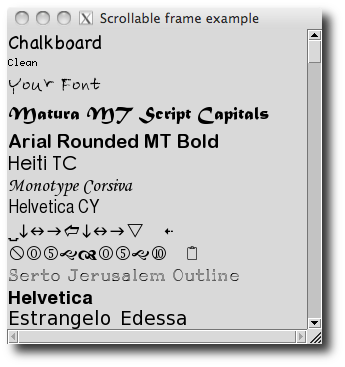
\includegraphics[width=.4\textwidth]{fig-tcltk-all-fonts.png}
  \caption{A scrollable frame widget (cf. Example~\ref{ex:tcltk-scrollable-frame}) showing the available fonts on a system.}
  \label{fig:fig-tcltk-all-fonts}
\end{figure}


\paragraph{Font metrics}
The average character size is important in setting the width and height of some components. The can be found through the \function{tkfont.measure} and \function{tkfont.metrics} functions as follows:
\begin{Schunk}
\begin{Sinput}
 tmp <- tkfont.measure("TkTextFont",paste(c(0:9,LETTERS),collapse=""))
 fontWidth <- ceiling(as.numeric(tclvalue(tmp))/36)
 tmp <- tkfont.metrics("TkTextFont","linespace"=NULL)
 fontHeight <- as.numeric(tclvalue(tmp))
 c(width=fontWidth, height=fontHeight)
\end{Sinput}
\begin{Soutput}
 width height 
     9     16 
\end{Soutput}
\end{Schunk}


\subsection{Images}
\label{sec:tcltk:overview:images}


Many \pkg{tcltk} widgets, including both labels and buttons, can show
images. In these cases, either with or without an accompanying text
label. Constructing images to display is similar to constructing new fonts, in
that a new image object is created and can be reused by various
widgets. The \function{tkimage.create} function is used to create image
objects. The following command shows how an image object can be made from the
file \code{tclp.gif} in the current directory:

\begin{Schunk}
\begin{Sinput}
 tkimage.create("photo", "::img::tclLogo", file = "tclp.gif")
\end{Sinput}
\begin{Soutput}
<Tcl> ::img::tclLogo 
\end{Soutput}
\end{Schunk}


The first argument, \qcode{photo} specifies that a full color image is
being used. This option could also be \qcode{bitmap} but that is more
a legacy option. The second argument specifies the name of the
object. We follow the advice of the \TK\/ manual and preface the name
with \code{::img::} so that we don't inadvertently overwrite any
existing \TCL\/ commands. The third argument
\argument{file}{tkimage.create} specifies the graphic file. The basic
\TK\/ \code{image} command only can show GIF and PPM/PNM
images. Unfortunately, not many \R\/ devices output in these
formats. (The \code{GDD} device driver can.) One may need system
utilities to convert to the allowable formats.

To use the image, one can specify the name for the \option{image}{ttklabel} option.
\begin{Schunk}
\begin{Sinput}
 l <- ttklabel(w, image="::img::tclLogo", text="logo text", 
               compound = "top")
\end{Sinput}
\end{Schunk}
By default the text will not show. The \argument{compound}{ttklabel} argument takes a value of either \qcode{text}, \qcode{image} (default), \qcode{center}, \qcode{top}, \qcode{left}, \qcode{bottom}, or \qcode{right} specifying where the label is in relation to the text.

\paragraph{Image manipulation}
Once an image is created, there are several options to manipulate the
image. These are found in the \TK\/ man page for \code{photo}, not
\code{image}. For instance, to change the palette so that instead of
\code{fullcolor} only 16 shades of gray are used to display the icon,
one could issue the command
\begin{Schunk}
\begin{Sinput}
 tkconfigure("::img::tclLogo", palette=16)
\end{Sinput}
\end{Schunk}

Another useful manipulation to draw attention to an image is to change the \code{gamma} value when something happens, such as a mouse-over event.


\subsection{Themes}
\label{sec:tcltk:overview:themes}


%% themes -- ttkframe
The themed widgets have a style that determines how they are drawn. The separation of style properties from the widget, as opposed to having these set for each construction of a widget, makes it much easier to change the look of a GUI and easier to maintain the code. A collection of styles makes up a theme. The available themes depend on the system. The default theme should enable a GUI to have the native look and feel of the operating system. (This was definitely not the case for the older \TK\/ widgets.) There is no built in command to return the theme, so we use \code{.Tcl} to call the appropriate \TCL\/ command. The \code{names} sub command will return the available themes and the \code{use} sub command can be used to set the theme.

\begin{Schunk}
\begin{Sinput}
 .Tcl("ttk::style theme names")
\end{Sinput}
\begin{Soutput}
<Tcl> aqua clam alt default classic 
\end{Soutput}
\begin{Sinput}
 .Tcl("ttk::style theme use classic")
\end{Sinput}
\end{Schunk}

The writing of themes will not be covered, but in Example~\ref{ex-tcltk-toolbar} we show how to create a new style for a button.

The example we have shown so far, would not look quite right, as the toplevel window is not a themed widget. To work around that, a \function{ttkframe} widget is usually used to hold the child components of the top-level window. The following shows how to place a frame inside the window, with some arguments to be explained later that allow it to act reasonably if the window is resized.
\begin{Schunk}
\begin{Sinput}
 w <- tktoplevel()
 f <- ttkframe(w, padding=c(3,3,12,12))  # a little breathing room
 tkpack(f, expand=TRUE, fill="both")     # handle window expansion
 l <- ttklabel(f, image="::img::tclLogo", text="label", compound="top")
 tkpack(l)
\end{Sinput}
\end{Schunk}

\subsection{Window properties and state: \code{tkwinfo}}
\label{sec:tcltk:overview:widget-properties}

Widgets have options which can be set through \code{tkconfigure} and
additionally, when mapped, the ``window'' they are rendered to has
properties, such as a class or size. These properties are queried
through the \function{tkwinfo} function.  There are several such
properties, and may take different forms. If the API is of the form

\begin{quotation}
\texttt{winfo subcommand\_name window}  
\end{quotation}
the specification to \function{tkwinfo} is in the same order (the widget is not the first argument). For instance, the class of a label is returned by the \texttt{class} subcommand as

\begin{Schunk}
\begin{Sinput}
 tkwinfo("class", l)
\end{Sinput}
\begin{Soutput}
<Tcl> TLabel 
\end{Soutput}
\end{Schunk}

The window, in this example \texttt{l}, can be specified as an \R\/ object, or by its character ID. This is useful, as the return value of some functions is the ID. For instance, the \texttt{children} subcommand returns IDs. Below the \code{as.character} function will coerce these into a vector of IDs.

\begin{Schunk}
\begin{Sinput}
 (children <- tkwinfo("children",f))
\end{Sinput}
\begin{Soutput}
<Tcl> .3.1.1 
\end{Soutput}
\begin{Sinput}
 sapply(as.character(children), function(i) tkwinfo("class", i))
\end{Sinput}
\begin{Soutput}
$`.3.1.1`
<Tcl> TLabel 
\end{Soutput}
\end{Schunk}

There are several possible subcommands, here we list a few. The
\subcommand{geometry}{tkwinfo} sub command returns the location and
size of the wigets' window in the form \code{width x height + x + y};
the sub commands \subcommand{height}{tkwinfo},
\subcommand{width}{tkwinfo}, \subcommand{x}{tkwinfo}, or
\subcommand{y}{tkwinfo} can be used to return just those parts. The
\subcommand{exists}{tkwinfo} command returns 1 (\code{TRUE}) if the
window exists and 0 otherwise; the \subcommand{ismapped}{tkwinfo} sub
command returns 1 or 0 if the window is currently mapped (drawn); the
\subcommand{viewable}{tkwinfo} sub command is similar, only it checks
that all parent windows are also mapped.  For traversing the widget
heirarchy, one has available the \subcommand{parent}{tkwinfo} sub
command which returns the immediate parent of the component,
\subcommand{toplevel}{tkwinfo} which returns the ID of the top-level
window, and \subcommand{children}{tkwinfo} which returns the IDs of
all the immediate child components, if the object is a container, such
as a top-level window.



\section{Events and Callbacks}
\label{sec:tcltk:overview:events-callbacks}

The button widget has the \code{command} option for assigning a callback for when the user clicks the mouse button on the button. In addition to this, one can specify callbacks for many other events that the user may initiate. 


\subsection{Callbacks}
\label{sec:tcltk:callbacks}
%% \XXX{ use of tcl(``eval'',''break'') to avoid calling subsequent callbacks} -- doesn't work
%% See PD's comments here on callbacks http://article.gmane.org/gmane.comp.lang.r.general/136705

The \pkg{tcltk} package implements callbacks in a manner different
from \TK, as the callback functions are \R\/ functions, not \TK\/
procedures. This is much more convenient, but introduces some slight
differences.  In \pkg{tcltk} these callbacks can be expressions
(unevaluated calls) or functions. We use only the latter, for more
clarity. The basic callback function need not have any arguments. For
instance, here we show how to print a message when the user clicks a
button:
\begin{Schunk}
\begin{Sinput}
 w <- tktoplevel()
 callback <- function() print("hi")
 b <- ttkbutton(w, text="Click me", command = callback)
  tkpack(b)
\end{Sinput}
\end{Schunk}


%% scope of callback?
The callback's return value is generally not important, although we
shall see with validation in Section~\ref{sec:tcltk:entry-widgets}, it
can matter. This is not the case in \Tk. As well, in \Tk\/ callbacks
are evaluated in the global environment, but this is not so in
\pkg{tcltk}.

\begin{Schunk}
\begin{Soutput}
<Tcl> .w 
\end{Soutput}
\begin{Soutput}
<Tcl> .w.b 
\end{Soutput}
\end{Schunk}
\subsection{Events}
\label{sec:tcltk:events}

%% (Unlike \pkg{RGtk2}, that the event triggers a widget to emit a signal that a callback listens for is notneeded)

When a user interacts with a GUI, they initiate events. The \pkg{tcltk} package allows the programmer to bind callbacks to these events, through the \function{tkbind} function. This function is called as \code{tkbind(tag, events, command)}. The \code{command} is a callback, as described above.

The \code{tag} argument allows for quite a bit of flexibility. It can be:

\begin{description}
\item[the name of a widget] in which the command will be bound to that widget;
\item[q top-level window] in which case the command will be be bound to the event for the window and all its internal widgets;

\item[a class of widget] such as \qcode{TButton}, in which case all such widgets will get the binding; or 
\item[the value \qcode{all}] in which case all widgets in the application will get the binding.
\end{description}
%% possible events
%% keys
The possible events (or sequences of events) vary from widget to widget. Events can be specified in a few ways. A single keypress event, can be assigned by specifying the ASCII character generated. For instance, to bind to  \kbd{C} for the ``Click me'' button above using the same callback could be done with
\begin{Schunk}
\begin{Sinput}
  tkbind(b, "C", callback)
  tkfocus(b)
\end{Sinput}
\end{Schunk}
The \function{tkfocus} function is used to set the focus to the button so that it will receive the keypress.

%% tkbind(widget,''<modifier-modifier-type-detail'>'', command)
\paragraph{Events with modifiers}
More complicated events can be described with the pattern 

\begin{quotation}
\code{\Event{modifier-modifier-type-detail}}.   
\end{quotation}

Examples are \code{\Event{KeyPress}},  \code{\Event{ButtonPress}}, \code{\Event{Double-Button-1}},  or \code{\Event{Control-c}}.
The full list of modifiers and types are described in the man page for \code{bind}. Some familiar modifiers are \code{Control}, \code{Alt}, \code{Button1} (or its shortening \code{B1}), \code{Double} and \code{Triple}. The event types are the standard X event types along with some abbreviations. These are also listed in the \code{bind} man page. Some commonly used ones are \code{ButtonPress}, \code{ButtonRelease}, \code{KeyPress}, \code{KeyRelease}, \code{FocusIn}, and \code{FocusOut}. The detail may be a button number or key, such as \code{a} or \code{C}.

\paragraph{Window manager events}
Some events are based on window manager events. The \Event{Configure}
event happens when a component is resized. The \Event{Map} and
\Event{Unmap} events happen when a component is drawn or undrawn.

\paragraph{Virtual events}
Finally, the event may be a ``virtual event.'' These are represented with \code{\VirtualEvent{EventName}}. There are predefined virtual events listed in the \code{event} man page. These include \code{\VirtualEvent{MenuSelect}} when working with menus,  \code{\VirtualEvent{Modified}} for text widgets, \code{\VirtualEvent{Selection}} for text widgets, and \code{\VirtualEvent{Cut}}, \code{\VirtualEvent{Copy}} and \code{\VirtualEvent{Paste}} for working with the clipboard. New virtual events can be produced with the \code{tkevent.add} function. This takes atleast two arguments, an event name and a sequence that will initiate that event. The \code{event} man page has these examples coming from the Emacs world:
\begin{Schunk}
\begin{Sinput}
  tkevent.add("<<Paste>>", "<Control-y>")
  tkevent.add("<<Save>>", "<Control-x><Control-s>")
\end{Sinput}
\end{Schunk}
In addition to virtual events occuring when the sequence is performed, the \function{tkevent.generate} can be used to force an event for a widget. This function requires a widget (or its ID) and the event name. Other options can be used to specify substitution values, described below. To illustrate, this command will generate the \code{\VirtualEvent{Save}} event for the button \code{b}:
\begin{Schunk}
\begin{Sinput}
 tkevent.generate(b, "<<Save>>")
\end{Sinput}
\end{Schunk}



In \pkg{tcltk} only one callback can be associated with a widget and event through the call \code{tkbind(widget,event,callback)}. (Although, callbacks for the widget associated with classes or toplevel windows can differ.) Calling \code{tkbind} another time will replace the callback. To remove a callback, simply assign a new callback which does nothing.~\footnote{This event handling can prevent being able to port some \Tk\/ code into \pkg{tcltk}. In those cases, one may consider sourcing in \Tcl\/ code directly.}



\subsection{\% Substitutions}
\label{sec:tcltk-percent-substitutions}
\TK\/ provides a mechanism called \defn{percent substitution} to pass
information about the event to callbacks bound to the event. The basic
idea is that in the \TCL\/ callback expressions of the type \code{\%X}
for different characters \code{X} will replaced by values coming from
the event. In \pkg{tcltk}, if the callback function has an argument
\code{X}, then that variable will correspond to the value specified by
\code{\%X}. The complete list of substitutions is in the \code{bind}
man page. Useful ones are \code{x} and \code{X} to specify the
relative or absolute $x$-postion of a mouse click (the difference can
be found through the \code{rootx} property of a widget), \code{y} and
\code{Y} for the $y$ position, \code{k} and \code{K} for the keycode
(ASCII) and key symbol of a \Event{KeyPress} event, and \code{W} to
refer to the ID of the widget that signaled the event the callback is
bound to. Example~\ref{ex-tcltk-dnd} will illustrate some of these.

%% After
\paragraph{The after command}
The \TCL\/ command \code{after} will execute a command after a certain delay (specified in milliseconds as an integer) while not interupting the control flow while it waits for its delay. The function is called in a manner like:
\begin{Schunk}
  \begin{Sinput}
afterID <- tcl("after", 1000, function() print("1 second passed"))    
  \end{Sinput}
\end{Schunk}
The ID returned by \code{after} may be used to cancel the command before it executes.




\begin{example}{Drag and Drop}{ex-tcltk-dnd}
This example shows how to implement drag and drop between two widgets. Steps are needed to make a widget a drop source, and other steps are needed to make a widget a drop target. The basic idea is that when a value is being dragged, virtual events are generated for the widget the cursor is over. If that widget has callbacks bound to these events, then the drag and drop can be processed. The idea for the code below originated with \url{http://wiki.tcl.tk/416}.


To begin, we create a simple GUI to hold three widgets. We use buttons
for drag and drop, but only because we haven't yet discussed more
natural widgets such as the text widgets. 

\begin{Schunk}
\begin{Sinput}
 w <- tktoplevel()
 bDrag <- ttkbutton(w, text="Drag me")
 bDrop <- ttkbutton(w, text="Drop here")
 tkpack(bDrag)
 tkpack(ttklabel(w, text="Drag over me"))
 tkpack(bDrop)
\end{Sinput}
\end{Schunk}


Before beginning, we define three global variables that can be shared
among drop sources to keep track of the drag and drop state. A more
elegant example might store these in an environment.
\begin{Schunk}
\begin{Sinput}
 .dragging <- FALSE                      # currently dragging?
 .lastWidgetID <- ""                     # last widget dragged over
 .dragValue <- ""                        # value to transfer
\end{Sinput}
\end{Schunk}


To set up a drag source, we bind to three events: a mouse button press, mouse motion, and a button release. For the button press, we set the values of the three global variables.
\begin{Schunk}
\begin{Sinput}
 tkbind(bDrag,"<ButtonPress-1>",function(W) {
   .dragging <<-  TRUE
   .lastWidgetID <<- as.character(W)
   .dragValue <<- as.character(tkcget(W,text=NULL))
 })
\end{Sinput}
\end{Schunk}


For mouse motion, we do several things. First we set the cursor to
indicate a drag operation. The choice of cursor is a bit outdated. The
commented code shows how one can put in a custom cursor from an xbm
file, but this doesn't work for all platforms (e.g.,  OS X). After setting the cursor, we find the ID of the widget the cursor is over. This uses \function{tkwinfo} to find the widget containing the $x,y$-coordinates of the cursor position.  We then generate the \VirtualEvent{DragOver} virtual event for this widget, and if this widget is different from the previous last widget, we generate the \VirtualEvent{DragLeave} virtual event.

%%  ## This failed with OS X: "
%%  ##  .Tcl(paste(as.character(bDrag$ID),' configure -cursor "@', getwd(),'/cursor.xbm black"', sep=""))

\begin{Schunk}
\begin{Sinput}
 tkbind(bDrag,"<B1-Motion>",function(W,X,Y) {
   if(!.dragging) return()
   ## see cursor help page in API for more
   ## For custom cursors cf. http://wiki.tcl.tk/8674. 
   tkconfigure(W, cursor="coffee_mug")    # set cursor
 
   w = tkwinfo("containing", X, Y)       # widget mouse is over
   if(as.logical(tkwinfo("exists", w)))   # does widget exist?
     tkevent.generate(w, "<<DragOver>>")
 
   ## generate drag leave if we left last widget
   if(as.logical(tkwinfo("exists", w)) &&
      length(as.character(w)) > 0 &&
      length(as.character(.lastWidgetID)) > 0
      ) {
     if(as.character(w)[1] != .lastWidgetID) 
       tkevent.generate(.lastWidgetID, "<<DragLeave>>")
   }
   .lastWidgetID <<- as.character(w)
 })
\end{Sinput}
\end{Schunk}


Finally, if the button is released, we generate the virtual events
\VirtualEvent{DragLeave} and most importantly \VirtualEvent{DragDrop} for the
widget we are over.
\begin{Schunk}
\begin{Sinput}
  tkbind(bDrag,"<ButtonRelease-1>",function(W, X, Y) {
   if(!.dragging) return()
   w = tkwinfo("containing", X, Y)
     
   if(as.logical(tkwinfo("exists", w))) {
     tkevent.generate(w, "<<DragLeave>>")
     tkevent.generate(w, "<<DragDrop>>")
     tkconfigure(w, cursor="")
   }
   .dragging <<- FALSE
   tkconfigure(W, cursor="")
 })
\end{Sinput}
\end{Schunk}


To set up a drop target, we  bind callbacks for the virtual events generated above to the widget. For the \VirtualEvent{DragOver} event we make the widget \code{active} so that it appears ready to receive a drag value.
\begin{Schunk}
\begin{Sinput}
 tkbind(bDrop,"<<DragOver>>",function(W) {
   if(.dragging) 
     tkconfigure(W, default="active")
 })
\end{Sinput}
\end{Schunk}
If the drag event leaves the widget without dropping, we change the state back to \code{normal}.
\begin{Schunk}
\begin{Sinput}
 tkbind(bDrop,"<<DragLeave>>", function(W) {
   if(.dragging)  {
     tkconfigure(W, cursor="")
     tkconfigure(W, default="normal")  
    }
 })
\end{Sinput}
\end{Schunk}
Finally, if the \VirtualEvent{DragDrop} virtual event occurs, we set the widget value to that stored in the global variable \code{.dragValue}.
\begin{Schunk}
\begin{Sinput}
 tkbind(bDrop,"<<DragDrop>>", function(W) {
   tkconfigure(W, text=.dragValue)
   .dragValue <- ""
 })
\end{Sinput}
\end{Schunk}
\end{example}


\section{Rcmdr}
\label{sec:tcltk:rcmdr}

[Adding to the Rcmdr. Write me.]


\section{Other sources of documentation}
\label{sec:tcltk:other-sourc-docum}

%% Docs
In writing this chapter we used the a few primary resources. The \TK\/
API~\citep{TclTk:API} lays out the details of each widget in a clear
concise manner. There is an excellent tutorial demonstrating the
themed widgets by Mark Roseman~\citep{TclTk:Tutorial}.  The \TCL\/
language is written about in several books. We used the authorative
text by Welch, Jones and Hobbs~\citep{beedub}. The \pkg{tcltk} package
was described in three very informative articles by the package Peter
Dalgaard~\citep{Dalgaard-DSC}, \citep{Rnews:Dalgaard:2001a}, and
\citep{Rnews:Dalgaard:2002}. Finally, a number of examples of the
package compiled by James Wettenhall may be seen
at~\citep{Wettenhall}.



\chapter{Tcl Tk: Containers and Layout}
\label{sec:tcltk:basic-containers}
%% parent windows, frames etc.
%% Example

\section{Top-level windows}
\label{sec:top-level-windows}
%%\XXX{Window Styles}

%% constructor
Top level windows are created through the \function{tktoplevel}
constructor. The arguments \argument{width}{tktoplevel} and \argument{height}{tktoplevel} may be
specified to give a requested size. Negative values means the window
will not request any size. Top-level windows can have a menubar specified through the \argument{menu}{tktoplevel} argument. Menus will be covered
in Section~\ref{sec:tcltk:menus}.

The \function{tkdestroy} function can be called to destroy the window
and its child components.

The \TK\/ command \code{wm} is used to interact with top-level
windows. This command has several subcommands, leading to \pkg{tcltk}
functions with names such as \function{tkwm.title}. This function is
used to set the window title. As with all such functions, either the
top-level window object, or its ID must be the first argument. In this
case, the new title is the second.

When a top-level window is constructed there is no option for it not
to be shown.  However, one can use the \function{tclServiceMode}
function to suspend/resume drawing of any widget through \TK. This
function takes a logical value to change the state. After a window is
drawn. To iconify an already drawn window can be down through the
\function{tkwm.withdraw} function and reversed with the
\function{tkwm.deiconify} function. Together these can be useful to
use in the construction of complicated GUIs, as the drawing of the
widgets can seem slow. (The same can be done through the
\function{tkwm.state} function with an option of \qcode{withdraw} or
\qcode{normal}.)
 
\paragraph{Window sizing}
The preferred size of a top-level window can be configured through the \code{width} and \code{height} options. The absolute size and position of a top-level window in pixels can be queried of specified through the \function{tkwm.geometry}
function. The geometry is specified as a string in the form \code{=wxh+x+y} (or \code{-}) where any of \code{=}, \code{wxh} or \code{+x+y} can be omitted. The value for \code{x} (if using \code{+})
indicates how many pixels to the right from the left edge should the window be
placed (if using \code{-} then the left side of the screen is used as
a reference). For \code{y} the top (or bottom) of the screen is the reference.

%% sizegrip
The \constructor{ttksizegrip} widget can be used to add a visual area (usually the lower right corner) for the user to grab on to with their mouse for resizing the window. On some OSes (e.g., Mac OS X) these are added by the window manager automatically. 

%%
The \function{tkwm.resizable} function can be used to prohibit the
resizing of a top-level window. The syntax allows either the width or
height to be constrained. The following command would  prevent
resizing of both the width and height of the toplevel window \code{w}. 

\begin{Schunk}
  \begin{Sinput}
tkwm.resizable(w, FALSE, FALSE)    # width first
  \end{Sinput}
\end{Schunk}

When a window is resized, you can constrain the minimun and maximum sizes with \function{tkwm.minsize} and \function{tkwm.maxsize}. The aspect ratio (width/height) can be set through \function{tkwm.aspect}.


%% overridedirect
For some uses it may be desirable to not have the window manager
decorate the window with a title bar etc. Tooltips, for example, can
be constructed using this approach. The command \subcommanda{wm
  overrideredirect}{tktoplevel}{logical} takes a logical value
indicating if the window should be decorated. Though, not all window
managers respect this.



%% binginds
\paragraph{bindings}
Bindings for top-level windows are shared by all of their child widgets. If a common binding is desired for all the children, then it need only be specified once for the top-level window.


%% wm protocol
The \function{tkwm.protocol} function is used to assign commands to
window manager events, most commonly, the delete event when the user
clicks the close button on the windows decorations. A top-level window
can be removed through the \function{tkdestroy} function, or through
the user clicking on the correct window decorations. When the window decoration is clicked, the window manager issues a \qcode{WM\_DELETE\_WINDOW} event. To bind to this, a command of thie form \code{tkwm.protocol(win,"WM\_DELETE\_WINDOW",  callback)} is used. 

To illustrate, if \code{w} is a top-level window, and
\code{e} a text entry widget
(cf. Section~\ref{sec:tcltk:multi-line-text}) then the following
snippet of code would check to see if the text widget has been
modified before closing the window. This uses a modal message box
described in Section~\ref{sec:tcltk:dialogs}.



\begin{Schunk}
\begin{Sinput}
 tkwm.protocol(w,"WM_DELETE_WINDOW", function() {
   modified <- tcl(e, "edit", "modified")
   if(as.logical(modified)) {
     response <- 
       tkmessageBox(icon="question",
                    message="Really close?",
                    detail="Changes need to be saved",
                    type="yesno",
                    parent=w)
     if(as.character(response) == "no")
       return()
   }
   tkdestroy(w)                          # otherwise close
 })
\end{Sinput}
\end{Schunk}

%% transient
Sometimes, say with dialogs, a top-level window should be related to
a different top-level window. The function \function{tkwm.transient}
allows one to specify the master window as its second argument. The
new window will mirror the state of the master window, including if
the master is withdrawn.

%% decorations

%% stack of windows
A window can be made to always be the topmost window through the
\code{attributes} subcommand of the \code{wm} command. However, there
is no direct \pkg{tcltk} function, so if \code{w} was to be on top, one would use the \function{tcl}
function as follows: 
\begin{Schunk}
\begin{Sinput}
tcl("wm", "attributes", w, topmost=TRUE)  
\end{Sinput}
\end{Schunk}

% When more than top-level window is in use, there is a stacking order
% describing how they are displayed. This stacking order is returned
% through the IDs of the windows through the \code{stackorder}
% subcommand of the \code{wm} command. There is no \pkg{tcltk} function
% for this, but the command \code{tcl("wm","stackorder", win)}, where
% \code{win} is the top-level window object will return the list.

% Stackign order of others; topmost
%% \begin{example}{A window constructor}{ex-tcltk-window}
%%\end{example}

\section{Frames}
\label{sec:tcltk:frames}

The \function{ttkframe} constructor produces a themable box container
that can be used to organize visible components within a GUI. It is
often the first thing packed within a top-level window.

The options include \option{width}{ttkframe} and
\option{height}{ttkframe} to set the requested size,
\option{borderwidth}{ttkframe} to specify a border around the frame of
a given width, and \option{relief}{ttkframe} to set the border
style. The value of \code{relief} is chosen from the default
\qcode{flat}, \qcode{groove}, \qcode{raised}, \qcode{ridge},
\qcode{solid}, or \qcode{sunken}.  The \option{padding}{ttkframe}
option can be used to to put space within the border between the
border and subsequent children.

\subsection{Label Frames}
\label{sec:tcltk:label-frames}

The \constructor{ttklabelframe} constructor produces a frame with an
optional label that can be used to set off and organize components of
a GUI. The label is set through the option
\option{text}{ttklabelframe}. Its position is determined by the option
\option{labelanchor}{ttklabelframe} taking values labeled by compass
headings (combinations of \code{n}, \code{e}, \code{w}, \code{s}. The
default is theme dependent, although typically \qcode{nw} (upper
left).

\paragraph{Separators}
To use a single line to separate out areas in a GUI, the
\constructor{ttkseparator} widget can be used. The lone
widget-specific option is \option{orient}{ttkseparator} which takes
values of \qcode{horizontal} (the default) or \qcode{vertical}. This
widget must be told to stretch when added to a container, as described
in the next section.

\section{Geometry Managers}
\label{sec:tcltk:geometry-managers}

\TCL\/ uses geometry managers to place child components within their
parent windows. There are three such managers, but we describe only
two, leaving the lower-level \code{place} command for the official documentation. The use of
geometry managers, allows \TK\/ to quickly reallocate space to a GUI's
components when it is resized.  The \function{tkpack} function will
place children into their parent in the box-like manner. We have seen
in several examples throughout the text, that through the use of
nested boxes, one can construct quite flexible layouts, and
Example~\ref{ex-tcltk-non-modal-dialog} will illustrate that once
again. When simultaneous horizontal and vertical alignment of child
components is desired, the \function{tkgrid} function can be used to
manage the components.

%% warn against mixing
A GUI may use a mix of pack and grid to mangage the child components,
but all siblings in the widget heirarchy must be managed the same
way. Mixing the two will typically result in a lockup of the \R\/
session.


\subsection{Pack}
\label{sec:tcltk:pack}

%%\XXX{Is there a method to redraw the GUI?}
%%\XXX{Comment that pack can pack into other parent?}

%% side
We have illustrated how \constructor{tkpack} can be used to manage how
child components are viewed within their parent. The basic usage
\code{tkpack(child)} will pack in the child components from top to
bottom. The \option{side}{tkpack} option can take a value of
\qcode{left}, \qcode{right}, \qcode{top} (default), or \qcode{bottom}
to adjust where the children are placed. These can be mixed and
matched, but sticking to just one direction is easier to
understand. Using nested frames is a more transparent approach.

\paragraph{after, before}
The \option{after}{tkpack} and \option{before}{tkpack} options can be
used to place the child before or after another component. These are
used as with \code{tkpack(child1, after=child2)}. The object
\code{child2} can be the \R\/ object or an ID. The latter might be
useful, say when all the children are listed using the command
\code{tkwinfo("children",parent)} which returns the IDs of the
immediate child components.

\paragraph{padding}

\begin{figure}
  \centering
  \begin{tabular}[c@{\quad}c@{\quad}]{ccc}
    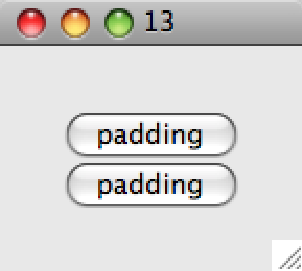
\includegraphics[width=.25\textwidth]{fig-pack-padding} &
    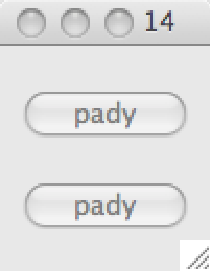
\includegraphics[width=.25\textwidth]{fig-pack-pady} &
    \includegraphics[width=.25\textwidth]{fig-pack-ipady}
  \end{tabular}
  \caption{Various ways to put padding between widgets using a box container and \function{tkpack}. The \code{padding} option for the box container puts padding around the cavity for all the widgets. The \code{pady} option for \function{tkpack} puts padding around the top and bottom on the border of each widget. The \code{ipady} option for \function{tkpack} puts padding within the top and bottom of the border for each child (modifying the theme under Mac OS X).}
  \label{fig:fig-pack-example}
\end{figure}

\begin{Schunk}
\begin{Sinput}
 ## Code to make padding/pady/ipady figure
 ## padding
 w <- tktoplevel();f <- ttkframe(w, padding=20 + 10);tkpack(f, expand=TRUE, fill="both")
 tkpack(ttkbutton(f, text="padding"))
 tkpack(ttkbutton(f, text="padding"))
 ##  pady outside border
 w <- tktoplevel();f <- ttkframe(w, padding=10);tkpack(f, expand=TRUE, fill="both")
 tkpack(ttkbutton(f, text="pady"), pady=10)
 tkpack(ttkbutton(f, text="pady"), pady=10)
 ## ipady within border
 w <- tktoplevel();f <- ttkframe(w, padding=10);tkpack(f, expand=TRUE, fill="both")
 tkpack(ttkbutton(f, text="ipady"), ipady=10)
 tkpack(ttkbutton(f, text="ipady"), ipady=10)
\end{Sinput}
\end{Schunk}

In addition to the \code{padding} option for a frame container, the
\option{ipadx}{tkpack}, \option{ipady}{tkpack}, \option{padx}{tkpack},
and \option{pady}{tkpack} options can be used to add space around the
child components. Figure~\ref{fig:fig-pack-example} has an
example. The \code{x} and \code{y} indicate left-right space or
top-bottom space. The \code{i} stands for internal padding that is
left on the sides or top and bottom of the child within the border,
for \code{padx} the external padding added around the border of the
child component. The value can be a single number or pair of numbers
for asymmetric padding.


This sample code shows how one can easily add padding around all the
children of the frame \code{f} using the
\subcommand{"configure"}{tkpack} subcommand.


\paragraph{Cavity model}
The packing algorithm, as described in the \Tk\/ documentation, is based
on arranging where to place a slave into the rectangular unallocated
space called a cavity. We use the nicer terms child component and box
to describe these. When a child is placed inside the box, say on the
top, the space allocated to the child is the rectangular space with
width given by the width of the box, and height the sum of the
requested height of the child plus twice the \code{ipady} amount (or
the sum if specified with two numbers). The packer then chooses the
dimension of the child component, again from the requested size plus
the \code{ipad} values for \code{x} and \code{y}. These two spacess
may, of course, have different dimensions.


\paragraph{anchor}
By default, the child  will be placed centered along the edge of
the box within the allocated space and blank space, if any, on both
sides.  If there is not enough space for the child in the allocated
space, the component can be drawn oddly. Enlarging the top-level
window can adjust this. When there is more space in the box than
requested by the child component, there are other options. The
\option{anchor}{tkpack} option can be used to anchor the child to a
place in the box by specifying one of the valid compass points
(eg. \code{"n"} or \code{"se"} leaving blank space around the
child. Padding between the child and the box can be set through the
\code{padx} and \code{pady} options.

\paragraph{expand, fill}
When there is more space in the original box than needed by the
children the extra space will be left blank unless some children have
the option \option{expand}{tkpack} set to \code{TRUE}. In this case,
the extra space is allocated evenly to each child with this set. The
\code{fill} option is often used when \code{expand} is set.  The
\option{fill}{tkpack} option is used to base the size of the child on
the available cavity in the box -- not on the requested size of the
child. The \code{fill} option can be \qcode{x}, \qcode{y} or
\qcode{both}. The former expanding the child's size in just one
direction, the latter in both.

\paragraph{forget}
Child components can be forgotten by the window manager, unmapping them but not destroying them, with the \subcommand{forget}{tkpack} subcommand, or the convenience function \function{tkpack.forget}. After a child component is removed this way, it can be re-placed in the GUI using a geometry manager. In \pkg{gWidgetstcltk} this is used to create a \code{gexpandgroup} container, as such a container is not provided by \TK.

\paragraph{Introspection}
The subcommand \subcommand{slaves}{tkpack} will return a list of the child components packed into a frame. Coercing these return values to character via \code{as.character} will produce the IDs of the child components. The subcommand \subcommand{info}{tkpack} will provide the packing info for a child.

\begin{example}{Packing dialog buttons}{ex-tcltk-pack}


This example shows how one can pack in action buttons, such as when a
dialog is created.

\begin{figure}
  \centering
  \includegraphics[width=.5\textwidth]{fig-tcltk-pack-buttons.png}
  \caption{Demonstration of using \code{tkpack} options showing
    effects of using the \code{side}
    and \code{padx} options to create
    dialog buttons.}
  \label{fig:tcltk-pack-buttons}
\end{figure}


The first example just uses \code{tkpack} without any arguments except
the side to indicate the buttons are packed in left to right, not top
to bottom.
\begin{Schunk}
\begin{Sinput}
 f1 <- ttklabelframe(f, text="plain vanilla")
 tkpack(f1, expand=TRUE, fill="x")
 l <- list(ttkbutton(f1, text="cancel"), ttkbutton(f1, text="ok"))
 QT <- sapply(l, function(i) tkpack(i, side="left"))
\end{Sinput}
\end{Schunk}

Typically the buttons are right justified. One way to do this is to
pack in using \code{side} with a value of \qcode{right}. This shows
how to use a blank expanding label to take up the space on the left.
\begin{Schunk}
\begin{Sinput}
 f2 <- ttklabelframe(f, text="push to right")
 tkpack(f2, expand=TRUE, fill="x")
 l <- list(ttkbutton(f2, text="cancel"), ttkbutton(f2, text="ok"))
 tkpack(ttklabel(f2, text=" "), expand=TRUE, fill="x", side="left")
 QT <- sapply(l, function(i) tkpack(i, side="left"))
\end{Sinput}
\end{Schunk}

Finally, we add in some padding to conform to Apple's design specification that such
buttons should have a 12 pixel separation.
\begin{Schunk}
\begin{Sinput}
 f3 <- ttklabelframe(f, text="push to right with space")
 tkpack(f3, expand=TRUE, fill="x")
 tkpack(ttklabel(f3, text=" "), expand=TRUE, fill="x", side="left")
 l <- list(ttkbutton(f3, text="cancel"), ttkbutton(f3, text="ok"))
 QT <- sapply(l, function(i) tkpack(i, side="left", padx=6))
\end{Sinput}
\end{Schunk}
\end{example}

\begin{example}{A non-modal dialog}{ex-tcltk-non-modal-dialog}
This example shows how to use  window, frames,  labels, buttons,
icons, packing and bindings to create a non-modal dialog. 

\begin{figure}
  \centering
  \includegraphics[width=.4\textwidth]{fig-tcltk-simple-dialog.png}
  \caption{Example of a simple dialog}
  \label{fig:fig-tcltk-simple-dialog}
\end{figure}

Although not written as a function, we set aside the values that would
be passed in were it.
\begin{Schunk}
\begin{Sinput}
 title <- "message dialog"
 message <- "Do you like tcltk so far?"
 parent <- NULL
 QT <- tkimage.create("photo", "::img::tclLogo", 
                      file = system.file("images","tclp.gif",
                        package="ProgGUIinR"))
\end{Sinput}
\end{Schunk}

The main top-level window is then given a title, then withdrawn while the GUI is created.
\begin{Schunk}
\begin{Sinput}
 w <- tktoplevel(); tkwm.title(w, title)
 tkwm.state(w, "withdrawn")
\end{Sinput}
\end{Schunk}

If the parent is non-null and is viewable, then the dialog is made
transient to a parent, The parent need not be a top-level window, so
\function{tkwinfo} if used to find the parent's top-level window. For Mac OS X, we use the \code{notify} attribute to bounce the dock icon until the mouse enters the window area.

\begin{Schunk}
\begin{Sinput}
 if(!is.null(parent)) {
   parentWin <- tkwinfo("toplevel", parent)
   if(as.logical(tkwinfo("viewable", parentWin))) {
     tkwm.transient(w, parent)
     tcl("wm","attributes",parentWin, notify=TRUE) # bounce
     tkbind(parentWin,"<Enter>", function() 
       tcl("wm","attributes",parentWin, notify=FALSE)) #stop
   }
 }
\end{Sinput}
\end{Schunk}
Finally, a frame is packed into the top-level window. Since we want the
frame to expand to fill all the space if the window is resized, we use \code{fill="both"}.
\begin{Schunk}
\begin{Sinput}
 ## frame for theme purposes, give some space
 f <- ttkframe(w,  padding=c(5,5,10,10))
 tkpack(f, expand=TRUE, fill="both")
\end{Sinput}
\end{Schunk}

We will use a standard layout for our dialog with an icon on the left,
a message and buttons on the right. We pack the icon into the left side of the frame,
\begin{Schunk}
\begin{Sinput}
 l <- ttklabel(f, image="::img::tclLogo", padding=5) # recycle
 tkpack(l,side="left")
\end{Sinput}
\end{Schunk}

A nested frame will be used to layout the message area and button area. Since the \function{tkpack} default is to pack in top to bottom, no \code{side} specification is made.
\begin{Schunk}
\begin{Sinput}
 f1 <- ttkframe(f)
 tkpack(f1, expand=TRUE, fill="both")
 #
 m <- ttklabel(f1, text=message)
 tkpack(m, expand=TRUE, fill="both")
\end{Sinput}
\end{Schunk}

The buttons have their own frame, as they are layed out horizontally. 
\begin{Schunk}
\begin{Sinput}
 f2 <- ttkframe(f1)
 tkpack(f2)
\end{Sinput}
\end{Schunk}
The callback function for the OK button prints a message then destroys the window.
\begin{Schunk}
\begin{Sinput}
 okCB <- function() {
   print("That's great")
   tkdestroy(w)
 }
 okButton <- ttkbutton(f2, text="OK", default="active")
\end{Sinput}
\end{Schunk}
We bind the callback to both a left mouse click on the button, and if the user presses \kbd{return} when the button has the focus. The \code{default="active"} argument, makes this button the one that gets the \code{Return} event when the \kbd{return} key is pressed.

\begin{Schunk}
\begin{Sinput}
 tkbind(okButton, "<Button-1>", okCB)
 tkbind(okButton, "<Return>", okCB)
 cancelButton <- ttkbutton(f2, text="Cancel", 
                           command=function() tkdestroy(w))
 tkpack(okButton, side="left", padx=12)  # give some space
 tkpack(cancelButton)
\end{Sinput}
\end{Schunk}

Now we bring the dialog back from its withdrawn state, fix the size and set the focus on the OK button.
\begin{Schunk}
\begin{Sinput}
 tkwm.state(w, "normal")
 tkwm.resizable(w, FALSE, FALSE)
 tkfocus(okButton)
\end{Sinput}
\end{Schunk}

Finally, the following bindings make the buttons look active when the keyboard focus is on them, generating a \code{FocusIn} event, then a \code{FocusOut} event. We make a binding for the top-level window, then within the callback check to see if the widget emitting the signal is of a themed button class.
\begin{Schunk}
\begin{Sinput}
 isTButton <- function(W)  
   as.character(tkwinfo("class",W)) == "TButton"
 tkbind(w,"<FocusIn>", function(W) {
   if(isTButton(W)) tkconfigure(W,default="active")
 })
 tkbind(w,"<FocusOut>", function(W) {
   if(isTButton(W)) tkconfigure(W,default="normal")
 })
\end{Sinput}
\end{Schunk}
\end{example}

\subsection{Grid}
\label{sec:tcltk:grid}
The \function{tkgrid} geometry manager is used to place child widgets in rows and columns. 
In its simplest usage, a command like
\begin{Schunk}
  \begin{Sinput}
tkgrid(child1, child2,..., childn)    
  \end{Sinput}
\end{Schunk}
will place the $n$ children in a new row, in columns 1 through $n$. However, the specific row and column can be specified through the \option{row}{tkgrid} and \option{column}{tkgrid} options. Counting of rows and columns starts with 0.  Spanning of multiple rows and columns can be specified with integers 2 or greater by the \option{rowspan}{tkgrid} and \option{colspan}{tkgrid} options. These options, and others can be adjusted through the \function{tkgrid.configure} function.


\paragraph{The tkgrid.rowconfigure, tkgrid.columnconfigure commands}
When the managed container is resized, the grid manager consults
weights that are assigned to each row and column to see how to
allocate the extra space. These weights are configured with the
\function{tkgrid.rowconfigure} and \function{tkgrid.columnconfigure}
functions through the option
\option{weight}{tkgrid.columnconfigure}, The weight is a value
between 0 and 1. If there are just two rows, and the first row has weight
$1/2$ and the second weight 1, then the extra space is allocated twice
as much for the second row. The specific row or column must also be
specified. Rows and columns are referenced starting with 0 not the usual \R-like 1. So to specify
a weight of 1 to the first row would be done with a command like:


\begin{Schunk}
\begin{Sinput}
 tkgrid.rowconfigure(parent, 0, weight=1)
\end{Sinput}
\end{Schunk}

\paragraph{The sticky option}
When more space is available then requested by the child component, the \option{sticky}{tkgrid} option can be used to place the widget into the grid. The value is a combination of the compass points \qcode{n},\qcode{e},\qcode{w}, and \qcode{s}. A specification \qcode{ns} will make the child component ``stick'' to the top and bottom of the cavity that is provided, similar to the \code{fill="y"} option for \function{tkgrid}. Similarly a value of \qcode{news} will make the child component expand in all the direction like \code{fill="both"}. A value of \qcode{w} will anchor the widget on the left side of the cavity

\paragraph{Padding}
As with \function{tkpack}, \function{tkgrid} has options
\option{ipadx}{tkgrid}, \option{ipady}{tkgrid}, \option{padx}{tkgrid},
and \option{padx}{tkgrid} to give internal and external space around a
child.

\paragraph{Size}
The function \function{tkgrid.size} will return the number of columns and rows of the specified parent container that is managed by a grid. This can be useful when trying to position child components through the options \code{row} and \code{column}.

\paragraph{Forget}
To remove a child from the parent, the \function{tkgrid.forget} function can be used with the child object as its argument.


\begin{example}{Using \function{tkgrid} and \function{tkpack} to draw some world flags}{ex-tcltk-flags}
This example shows how the \function{tkpack} the \function{tkgrid} geometry managers can be used to draw some of the world flags. For these, we consulted \url{https://www.cia.gov/library/publications/the-world-factbook/docs/flagsoftheworld.html}.


\begin{figure}
  \centering
  \begin{tabular}{cc}
    \includegraphics[width=.4\textwidth]{fig-tcltk-mali.png}
    & %%  \hfill
    \includegraphics[width=.5\textwidth]{fig-tcltk-lithuania.png}
    \\
    \includegraphics[width=.4\textwidth]{fig-tcltk-benin.png}
    &
    \includegraphics[width=.4\textwidth]{fig-tcltk-togo.png}
  \end{tabular}
  \caption{Example of world flags to illustrate \function{tkpack} and \function{tkgrid} usage. The Mali flag uses \code{expand=TRUE} to allocate space evenly, \code{fill="both"} to have the child fill the space and \code{side="left"} to place the children, whereas Lithuania uses \code{side="top"}. The Benin flag takes advantage of \code{tkgrid} to layout the colors in a grid. The left color has \code{rowspan=2} set. The Togo flag could be done using just \code{grid}, but a mix is demonstrated.}
  \label{fig:tcltk-flags}
\end{figure}



We will make the dimensions of the flags true to the flag proportions. These we found at \url{http://flagspot.net/flags/xf-size.html}. Here we define the proportions for the flags of interest.
\begin{Schunk}
\begin{Sinput}
 dims <- cbind(Benin=2:3, Cameroon=2:3,Guinea=2:3, Mali=2:3,
               Bolivia=2:3, Lithuania=1:2,Congo=2:3, Guyana=1:2,
               Togo= 2:3)
\end{Sinput}
\end{Schunk}

This is a convenience function to create \function{tkframes} with different background colors. We use \function{tkframe} here -- not \function{ttkframe} -- as it has a background property.
\begin{Schunk}
\begin{Sinput}
 makeColors <- function(parent)
   list(green  = tkframe(parent, background="green"),
        red    = tkframe(parent, background="red"),
        yellow = tkframe(parent, background="yellow"))
\end{Sinput}
\end{Schunk}

This convenience function packs a frame into a top-level window.
\begin{Schunk}
\begin{Sinput}
 makeTopLevel <- function(country) {
   w <- tktoplevel()
   tkwm.title(w, country)
   f <- ttkframe(w, padding=c(3,3,3,12))
   tkpack(f, expand=TRUE, fill="both")
   return(list(w=w, f= f, country=country))
 }
\end{Sinput}
\end{Schunk}
This function resizes the toplevel window and forces it to have a fixed proportion using the global \code{dims} defined previously.
\begin{Schunk}
\begin{Sinput}
 resizeWin <- function(win) {
   height <- 200;
   setWidth <- function(h)
     floor(h * dims[2, win$country] / dims[1, win$country])
   width <- setWidth(height)
   tkwm.geometry(win$w, paste(width, height, sep="x"))
   ## constrain the resize to flag proportions
   ## alternate to tkwm.aspect(w, a,b,c,d)
   tkbind(win$w, "<Configure>", function(W) {
     tl <- tkwinfo("toplevel",W)
     geo <- tclvalue(tkwm.geometry(tl))
     geo <- as.numeric(unlist(strsplit(geo,"[^[:digit:]]"))[1:2])
     tkwm.geometry(tl, paste(setWidth(geo[2]), geo[2], sep="x"))
   })
 }
\end{Sinput}
\end{Schunk}

Our first flags are  Cameroon (GRY), Guinea (RYG), and Mali (GYR). These are flags with 3 equal vertical strips of color. We use tkpack with \code{side="left"} to pack in the colors from left to right. The \code{expand=TRUE} option causes extra space to be allocated equally to the three children, preserving the equal sizes in this case.

\begin{Schunk}
\begin{Sinput}
 win <- makeTopLevel("Cameroon")
 w <- win$w; f <- win$f
 l <- makeColors(f)
 tkpack(l$green, l$red, l$yellow, expand=TRUE, 
   fill="both", side="left")
 resizeWin(win)
\end{Sinput}
\end{Schunk}

To create Guinea's flag we simply move the green strip to the end.
\begin{Schunk}
\begin{Sinput}
 ## Guinea just moves colors around
 tkpack("forget", l$green)
 tkpack(l$green, expand=TRUE, fill="both", side="left")
 tkwm.title(win$w, "Guinea")
\end{Sinput}
\end{Schunk}

For Mali, we flip the position of green and red. We pack them in relative to the yellow strip using the \code{before} and \code{after} options to \function{tkpack}.
\begin{Schunk}
\begin{Sinput}
 tkpack("forget", l$green)
 tkpack("forget", l$red)
 tkpack(l$green, before=l$yellow, expand=TRUE, fill="both", side="left")
 tkpack(l$red, after=l$yellow, expand=TRUE, fill="both", side="left")
 tkwm.title(win$w, "Mali")
\end{Sinput}
\end{Schunk}

Lithuania is similar, only the stripes run horizontally. We pack from top to bottom to achieve this.
\begin{Schunk}
\begin{Sinput}
 win <- makeTopLevel("Lithuania")
 l <- makeColors(win$f)
 tkpack(l$yellow, l$green, l$red, expand=TRUE, fill="both", side="top")
 resizeWin(win)
\end{Sinput}
\end{Schunk}

Benin's flag is better suited for the grid geometry manager. We use a combination of \code{rowspan} and \code{columnspan} to get the proper arrangement. In this case, the proportions of the colors are achieved through equal weights when we configure the row and columns.
\begin{Schunk}
\begin{Sinput}
 ## benin is better suited for grid
 win <- makeTopLevel("Benin")
 l <- makeColors(win$f)
 tkgrid(l$green,  row=0, column=0, rowspan=2,    sticky="news")
 tkgrid(l$yellow, row=0, column=1, columnspan=2, sticky="news")
 tkgrid(l$red,    row=1, column=1, columnspan=2, sticky="news")
 ## use grid in equal sizes to get spaing right
 tkgrid.rowconfigure(win$f, 0:1, weight=1)
 tkgrid.columnconfigure(win$f, 0:2, weight=1) 
 resizeWin(win)
\end{Sinput}
\end{Schunk}

Togo is trickier. We could use grid,  as above, with the proper
combinations of row and columnspan. Instead we do this less directly to illustrate the mixing of the \function{tkgrid} and \function{tkpack} geometry managers.

\begin{Schunk}
\begin{Sinput}
 win <- makeTopLevel("Togo")
 f <- win$f
 l <- makeColors(f)
 upperR <- ttkframe(f); bottom <- ttkframe(f)
 tkgrid(l$red, row=0, column=0, sticky="news")
 tkgrid(upperR, row=0, column=1, sticky="news")
 tkgrid(bottom, row=1, column=0, columnspan=2, sticky="news")
 l1 <- makeColors(upperR)
 tkpack(l1$yellow, expand=TRUE, fill="both", side="top")
 tkpack(l1$green, expand=TRUE, fill="both", side="top")
 l2 <- makeColors(bottom)
 tkpack(l2$yellow, expand=TRUE, fill="both", side="top")
 tkpack(l2$green, expand=TRUE, fill="both", side="top")
 tkgrid.rowconfigure(f, 0:1, weight=1)
 tkgrid.columnconfigure(f, 0, weight=8)
 tkgrid.columnconfigure(f, 1, weight=10)  # not quite uniform
 resizeWin(win)
\end{Sinput}
\end{Schunk}


\end{example}


\begin{example}{Using \function{tkgrid} to create a toolbar}{ex-tcltk-toolbar}




\TK\/ does not have a toolbar widget. Here we use \function{tkgrid} to
show how we can add one to a top-level window in a manner that is not
affected by resizing. We begin by packing a frame into a
top-level window.
\begin{Schunk}
\begin{Sinput}
 w <- tktoplevel(); tkwm.title(w, "Toolbar example")
 f <- ttkframe(w, padding=c(3,3,12,12))
 tkpack(f, expand=TRUE, fill="both")
\end{Sinput}
\end{Schunk}
Our example has two main containers: one to hold the toolbar buttons
and one to hold the main content.
\begin{Schunk}
\begin{Sinput}
 tbFrame <- ttkframe(f, padding=0)
 contentFrame <- ttkframe(f, padding=4)
\end{Sinput}
\end{Schunk}
The \function{tkgrid} geometry manager is used to place the toolbar at
the top, and the content frame below. The choice of sticky and the weights ensure that
the toolbar does not resize if the window does.
\begin{Schunk}
\begin{Sinput}
 tkgrid(tbFrame, row=0, column=0, sticky="we")
 tkgrid(contentFrame, row=1, column=0, sticky = "news")
 tkgrid.rowconfigure(f, 0, weight=0)
 tkgrid.rowconfigure(f, 1, weight=1)
 tkgrid.columnconfigure(f, 0, weight=1)
 ## some example to pack into the content area
 tkpack(ttklabel(contentFrame, text="Some content"))
\end{Sinput}
\end{Schunk}

Now to add some buttons to the toolbar. We first show how to create a
new style for a button, slightly modifiying the themed button to set
the font and padding, and eliminate the border if the OS allows. This
\code{makeIcon} function finds stock icons from the \pkg{gWidgets}
package.
\begin{Schunk}
\begin{Sinput}
 tcl("ttk::style","configure","Toolbar.TButton", 
     font="helvetica 12", padding=0, borderwidth=0)
 makeIcon <- function(parent, stockName, command=NULL) {
   iconFile <- system.file("images", 
                           paste(stockName,"gif",sep="."), 
                           package="gWidgets")
   if(nchar(iconFile) == 0) {
     b <- ttkbutton(parent, text=stockName, width=6)
   } else {
     iconName <- paste("::img::",stockName, sep="")
     tkimage.create("photo", iconName, file = iconFile)
     b <- ttkbutton(parent, image=iconName, 
                    style="Toolbar.TButton", text=stockName, 
                    compound="top", width=6)
     if(!is.null(command))
       tkconfigure(b, command=command)
   }
   return(b)
 }
\end{Sinput}
\end{Schunk}

To illustrate, we pack in some icons. Here we use \function{tkpack}.  
One does not use \function{tkpack} and \function{tkgrid} to manage
children of the same parent, but these are children of \code{tbFrame},
not \code{f}.
\begin{Schunk}
\begin{Sinput}
 tkpack(makeIcon(tbFrame, "ok"), side="left")
 tkpack(makeIcon(tbFrame, "quit"), side="left")
 tkpack(makeIcon(tbFrame, "cancel"), side="left")
\end{Sinput}
\end{Schunk}

These two bindings show how to slightly highlight the icon when the
mouse is over that button, so that the user has some extra feedback.
\begin{Schunk}
\begin{Sinput}
 changeGamma <- function(W, gamma=1.0) {
   if(as.character(tkwinfo("class",W)) == "TButton") {
     img <- tkcget(W,"image"=NULL)
     tkconfigure(img, gamma=gamma)
   
   }
 }
 tkbind(w,"<Enter>", function(W) changeGamma(W, gamma=0.5))
 tkbind(w,"<Leave>", function(W) changeGamma(W, gamma=1.0))
\end{Sinput}
\end{Schunk}

\begin{figure}
  \centering
  \includegraphics[width=.4\textwidth]{fig-tcltk-toolbar.png}
  \caption{Illustration of using \code{tkpack} to make a toolbar. }
  \label{fig:fig-tcltk-toolbar}
\end{figure}

\end{example}


\section{Other containers}
\label{sec:tcltk:other-containers}
\TK\/ provides just a few other basic containers, here we describe paned windows and notebooks.

\subsection{Paned Windows}
\label{sec:tcltk:paned-windows}

A paned window  is constructed by the function \constructor{ttkpanedwindow}. The primary option, outside of setting the requested width or height with \option{width}{ttkpanedwindow} and \option{height}{ttkpanedwindow}, is \option{orient}{ttkpanedwindow}, which takes a value of \qcode{vertical} (the default) or \qcode{horizontal}. This specifies how the children are stacked, and is opposite how the sash is drawn.

%% adding
The returned object can be used as a parent container, although one does not use the geometry managers to manage them. Instead, the \method{add}{ttkpandedwindow} command is used. For example:
\begin{Schunk}
\begin{Sinput}
 w <- tktoplevel(); tkwm.title(w, "Paned window example")
 pw <- ttkpanedwindow(w, orient="horizontal")
 tkpack(pw, expand=TRUE, fill="both")
 left <- ttklabel(pw, text="left"); right <- ttklabel(pw, text="right")
 #
 tkadd(pw, left, weight=1)
 tkadd(pw, right, weight=2)
\end{Sinput}
\end{Schunk}
When resizing which child gets the space is determined by the
associated \code{weight}, specified as an integer. The default uses
even weights.  Unlike \GTK\/ more than two children are allowed.

\paragraph{Forget}
The subcommand \subcommand{forget}{ttkpanedwindow} can be used to
unmanage a child component. For the paned window, we have no convenience function, so we call as follows:
\begin{Schunk}
\begin{Sinput}
 tcl(pw, "forget", right)
 tkadd(pw, right, weight=2) ## add back
\end{Sinput}
\end{Schunk}

\paragraph{Sash position}
The sash between two children can be adjusted through the subcommand
\subcommand{sashpos}{ttkpanedwindow}. The index of the sash needs
specifying, as there can be more than one. Counting starts at 0. The
value for \code{sashpos} is in terms of pixel width (or height) of the
paned window. The width can be returned as follows:
\begin{Schunk}
\begin{Sinput}
 tcl(pw, "sashpos", 0, 150)
\end{Sinput}
\begin{Soutput}
<Tcl> 59 
\end{Soutput}
\begin{Sinput}
 as.integer(tkwinfo("width", pw))  # or "height"
\end{Sinput}
\begin{Soutput}
[1] 71
\end{Soutput}
\end{Schunk}

\subsection{Notebooks}
\label{sec:tcltk:notebooks}

%% constructor
The \constructor{ttknotebook} constructor returns a notebook object that can be subsequently manipulated. In \TK\/ the object itself, becomes a command with the subcommands being important. There are no convenience functions for these, so we will use the \function{tcl} function directly.

Notebook pages can be added through the \subcommand{add}{ttknotebook} subcommand or inserted after a page through the \subcommand{insert}{ttknotebook} subcommand. The latter requires a tab ID to be specified, as described below. The tab label is configured similarly to \function{ttklabel} through the options \option{text}{ttknotebook} and the optional \option{image}{ttknotebook}, which if given has its placement determined by \option{compound}{ttknotebook}. 
The placement of the child component within the notebook page is manipulated similarly as \function{tkgrid} through the  \option{sticky}{ttknotebook} option with values specified through compass points. Extra padding around the child can be added through the \option{padding}{ttknotebook} option. Typically, the child components would be containers to hold more complicated layouts. 

\paragraph{Tab identifiers} %%integer (0-based), object (ID), "current", "end"
Many of the commands for a notebook require a specification of a desired tab. This can be given by index, starting at 0; by the values \code{"current"} or \code{"end"}; by the child object added to the tab, either as an \R\/ object or an ID; or in terms of $x$-$y$ coordinates in the form \code{"@x,y"} (likely found through a binding).

%% illustrate add, inser
To illustrate, if \code{nb} is a \code{ttknotebook} object, then these commands would add pages.
\begin{Schunk}
\begin{Sinput}
 iconFile <- system.file("images",paste("help","gif",sep="."),
                         package="gWidgets")
 iconName <- "::tcl::helpIcon"
 QT <- tkimage.create("photo", iconName, file = iconFile)
 l1 <- ttklabel(nb, text="label 1")
 l2 <- ttklabel(nb, text="label 2")
 tkadd(nb, l2, sticky="nswe", text="label 2", 
     image=iconName, compound="right")
 ## put l1 first (tabID is 0)
 tkinsert(nb, 0, l1, sticky="nswe", text="label 1")
\end{Sinput}
\end{Schunk}

There are several useful subcommands to extract information from the notebook object.  For instance, \code{index} to return the page index (0-based), \code{tabs} to return the page IDs, \code{select} to select the displayed page, and \code{forget} to remove a page from the notebook. Except for \code{tabs}, these require a specification of a tab ID.
\begin{Schunk}
\begin{Sinput}
 tcl(nb, "index", "current")           # current page for tabID
\end{Sinput}
\begin{Soutput}
<Tcl> 1 
\end{Soutput}
\begin{Sinput}
 length(as.character(tcl(nb,"tabs")))  # number of pages
\end{Sinput}
\begin{Soutput}
[1] 2
\end{Soutput}
\begin{Sinput}
 tcl(nb, "select", 0)                  # select viewable page by index
 tcl(nb, "forget", l1)                 # forget removes page from notebook
 tcl(nb, "add", l1)                    # can be managed again.
\end{Sinput}
\end{Schunk}


%% keyboard
The notebook state can be manipulated through the keyboard, provided traversal is enabled. This can be done through
\begin{Schunk}
\begin{Sinput}
 QT <- tcl("ttk::notebook::enableTraversal", nb)
\end{Sinput}
\end{Schunk}

If enabled, the shortcuts such as \kbd{control-tab} to move to the
next tab are imlemented. If new pages are added or inserted with the
option \option{underline}{ttknotebook}, which takes an integer value
(0-based) specifying which character in the label is underlined, then
a keyboard accelerator is added for that letter.

\paragraph{bindings}
%% virtualevent
Beyond the usual events, the 
notebook widget also generates a \VirtualEvent{NotebookTabChanged} virtual event after a new tab is selected. 

%% limitations: no easy way to get close buttons (to me anyways); no graceful way to handle too man tabs.
The notebook container in \TK\/ has a few limitations. For instance,
there is no graceful management of too many tabs, as there is with
\GTK, as well there is no easy way to implement close buttons as an
icon.


\chapter{Tcl Tk: Widgets}
\label{sec:tcltk:widgets}

\Tk\/ has widgets for the common GUI controls. As mentioned in
Chapter~\ref{sec:tcltk:overview}, the constructors for these widgets
call the function \function{tkwidget} which calls the appropriate
\TK\/ command and adds in extra information including an ID and an
environment. As with labels and buttons, one primarily uses
\function{tkconfigure} and \function{tkcget} to set and get properties
of the widget.

The label, button and image constructors were discussed in
Section~\ref{sec:tcltk:overview}. For buttons and labels, we saw that
a \TCL\/ variable can be used to store the data for a widget.


\section{Selection Widgets}
\label{sec:tcltk:selection-widgets}

This section covers the many different ways to present data for the
user to select a value. The widgets can use \TCL\/ variables to refer to the value that is displayed or that the user selects. 
Recall, these were constructred through \function{tclVar} and manipulated rhough \code{tclvalue}.
For example, a logical value can be stored as
\begin{Schunk}
\begin{Sinput}
 value <- tclVar(TRUE)
 tclvalue(value) <- FALSE
 tclvalue(value)
\end{Sinput}
\begin{Soutput}
[1] "0"
\end{Soutput}
\end{Schunk}
As \code{tclvalue} coerces the logical into the  character string  \qcode{0} or \qcode{1}, some coercion may be desired.

\subsection{Checkbutton}
\label{sec:tcltk:checkboxes}

The \constructor{ttkcheckbutton} constructor returns a check button
object. The checkbuttons value (\code{TRUE} or \code{FALSE}) is linked
to a \TCL\/ variable which can be specified using a logical value.
The checkbutton label can also be specified through a \TCL\/ variable
using the \option{textvariable}{ttkcheckbutton} option.  Alternately,
as with the \code{ttklabel} constructor, the label can be specified
through the \option{text}{ttkcheckbutton} option. This allows one to
specify an image as well and arrange its display, as is done with
\function{ttklabel}, using the \option{compound}{ttkcheckbutton}
option.

The \option{command}{ttkcheckbutton} argument is used at construction
time to specify a callback when the button is clicked. The callback is
called when the state toggles, so often a callback considers the
state of the widget before proceeding. Binding through \code{\Event{Button-1}} can be
problematic, as the callback is called before the variable is updated,
use \code{\Event{ButtonRelease-1}}.

For example, if \code{f} is a frame, we can create a new check button with the following:

\begin{Schunk}
\begin{Sinput}
 value <- tclVar(TRUE)
 callback <- function() print(tclvalue(value))     # uses global
 labelVar <- tclVar("check button label")
 cb <- ttkcheckbutton(f, variable=value, 
                      textvariable=labelVar, command=callback)
 tkpack(cb)
\end{Sinput}
\end{Schunk}

To avoid using a global variable is not trivial here. There is no easy way to pass user data through to the callback, and there is no easy way to get the \R\/ object from the values passed through the \% substitution values. The variable holding the value can be found through
\begin{Schunk}
\begin{Sinput}
 tkcget(cb, "variable"=NULL)
\end{Sinput}
\begin{Soutput}
<Tcl> ::RTcl3 
\end{Soutput}
\end{Schunk}

But manipulating that is difficult.  A more general strategy within
\R\/ would be to use a function closure to encapsulate the variables
or an environment to store the global values.


% This following code is one way, certainly not the best, to add a callback that allows one to pass in user data. 
% <<addBinding>>=
% addBinding <- function(widget, event="<Button-1>", cb, userData=NULL) {
%   subArgs <- names(formals(cb)[-1])
%   subArgs <- if(length(subArgs)) paste(subArgs, collapse=",") else ""
%   expr <- paste("function(",subArgs,") {",
%                 "h <- list(widget=widget, userData=userData);",
%                 "cb(h",
%                 if(subArgs != "") paste(",",subArgs, collase=""),
%                 ")}", sep="")
%   callback <- eval(parse(text=expr))
%   tkbind(widget,event,callback)
% }
% @ 
% The following uses \code{addBinding} to toggle the checkbutton value when the \kbd{return} key is pressed when the widget has the focus.
% <<>>=
% addBinding(widget=cb, event="<Return>",
%            cb= function(h)  {
%              tclvalue(h$userData) <- !as.numeric(tclvalue(h$userData))
%            },
%            userData=value)
% @ 

% <<>>=
% addBinding(widget=cb, userData=value, event="<Return>",
%            cb= function(h)  {
%              tclvalue(h$userData) <- !as.numeric(tclvalue(h$userData))
%            })
% @ 

\subsection{Radio Buttons}
\label{sec:tcltk:radio-buttons}

Radiobuttons are checkbuttons linked through a shared \TCL\/ variable. Each button is constructed
through the \constructor{ttkradiobutton} constructor. Each button has a value and a
label, which need not be the same. The variable refers to the
value. As with labels, the radio button labels may be specified
through a text variable or the \option{text}{ttkradiobutton} option,
in which case, as with a \code{ttklabel}, an image may also be incorporated through the
\option{image}{ttkradiobutton} and \option{compound}{ttkradiobutton} options. In \TK\/ the placement of the buttons is managed by the programmer.


This small example shows how radio buttons could be used for selection
of an alternative hypothesis, assuming \code{f} is a parent container.

\begin{Schunk}
\begin{Sinput}
 values <- c("less", "greater", "two.sided")
 var <- tclVar(values[3])                # initial value
 callback <- function() print(tclvalue(var))
 for(i in values) {
   rb <- ttkradiobutton(f, text=i, variable=var, value=i,
                        command=callback)
   tkpack(rb, side="top", anchor="w")
 }
\end{Sinput}
\end{Schunk}


\subsection{Comboboxes}
\label{sec:tcltk:comboboxes}

The \constructor{ttkcombobox} constructor returns a combobox object to
select from a list of values, or with the appropriate option, allowing
the user to specify a value. Like radiobuttons and checkbuttons, the
value of the combobox can be specified using a \TCL\/ variable to the
option \option{textvariable}{ttkcombobox}, making the getting and
setting of the displayed value straightforward. The possible values to
select from are specified as a character vector through the
\option{values}{ttkcombobox} option. (This may require one to coerce
the results to the desired class.) Unlike \GTK\/ there is no option to
include images in the displayed text. One can adjust the alignment
through the \option{justify}{ttkcombobox} options.  By default, a user
can add in additional values through the entry widget part of the
combobox. The \option{state}{ttkcombobox} option controls this, with
the default  \qcode{normal} and the value \qcode{readonly} as an
alternative.

To illustrate, again suppose \code{f} is a parent container. Then we
begin by defining some values to choose from and a \TCL\/ variable.


\begin{Schunk}
\begin{Sinput}
 values <- rownames(mtcars)
 var <- tclVar(values[1])
\end{Sinput}
\end{Schunk}

The constructor call is as follows:
\begin{Schunk}
\begin{Sinput}
 cb <- ttkcombobox(f,
                   values=values,
                   textvariable=var,
                   state="normal", # or "readonly"
                   justify="left")
 tkpack(cb)
\end{Sinput}
\end{Schunk}


The possible values the user can select from can be configured after
construction through the \option{values}{ttkcombobox} option.
\begin{Schunk}
\begin{Sinput}
 tkconfigure(cb, values=tolower(values))
\end{Sinput}
\end{Schunk}


\paragraph{Setting the value}
Setting values can be done through the \TCL\/ variable, or by value or index (0-based) using the \subcommand{set}{ttkcombobox} sub command through \function{tkset} or the \subcommand{current}{ttkcombobox} sub command.

\begin{Schunk}
\begin{Sinput}
 tclvalue(var) <- values[2]            # using tcl variable
 tkset(cb, values[4])                  # by value
 tcl(cb, "current", 4)                 # by index
\end{Sinput}
\end{Schunk}
The values can also be retrieved in this manner, but coercing into a usable \R\/ object is not supported in general.

\paragraph{Getting the value}
One can retrieve the selected object in various ways: from the \TCL\/ variable. Additionally, the \subcommand{get}{ttkcombobox} subcommand can be used through \function{tkget}.

\begin{Schunk}
\begin{Sinput}
 tclvalue(var)                           # TCL variable
\end{Sinput}
\begin{Soutput}
[1] "hornet sportabout"
\end{Soutput}
\begin{Sinput}
 tkget(cb)                               # get subcommand
\end{Sinput}
\begin{Soutput}
<Tcl> hornet sportabout 
\end{Soutput}
\begin{Sinput}
 tcl(cb, "current")                      # 0-based index
\end{Sinput}
\begin{Soutput}
<Tcl> 4 
\end{Soutput}
\end{Schunk}

\paragraph{Events}
The virtual event \VirtualEvent{ComboboxSelected} occurs with selection. When the combobox may be edited, a user may expect some action when the \kbd{return} key is pressed. This triggers a \Event{Return} event, so to bind to this event, one can do something like the following:

\begin{Schunk}
\begin{Sinput}
 tkbind(cb, "<Return>", function(W) {
   val <- tkget(W)
   cat(as.character(val), "\n")
 })
\end{Sinput}
\end{Schunk}

For editable comboboxes, the widget also supports some of the
\function{ttkentry} commands discussed in
Section~\ref{ex:tcltk:entry-widgets}.


% \subsection{Listboxes}
% \label{sec:tcltk:listboxes}

% The \constructor{tklistbox} is a non-themed widget that can be used
% to select from a table of values. One can do a similar thing using
% the more general tree widget provided by \function{ttktreeview}
% widget, but the listbox is more convenient to use.



\subsection{Scale widgets}
\label{sec:tcltk:scale-widgets}

The \constructor{ttkscale} constructor to produce a themable scale (slider) control is missing. You can define your own:
\begin{Schunk}
\begin{Sinput}
 ttkscale <- function(parent, ...) tkwidget(parent, "ttk::scale", ...)
\end{Sinput}
\end{Schunk}

The orientation is set through the option \option{orient}{ttkscale}
taking values of \qcode{horizontal} (the default) or
\qcode{vertical}. For sizing the slider, the \option{length}{ttkscale}
option is available.  To set the range, the basic options are
\option{from}{ttkscale} and \option{to}{ttkscale} to set the
range. There is no \code{by} option as of \TK\/ 8.5. The constructor
\constructor{tkscale}, for a non-themable slider, has the option
\option{resolution}{tkscale} to set that. The
\option{variable}{ttkscale} option is used for specifying a \TCL\/
variable to record the value of the slider. Otherwise the
\option{value}{ttkscale} option is available.  The \function{tkget} and \function{tkset} function (using the 
\subcommand{get}{ttkscale} and \subcommand{set}{ttkscale} sub commands)
can be used to get and set the value shown. They are used in the same
manner as the same subcommands for a combobox. Again, the
\option{command}{ttkscale} option can be used to specify a callback
for when the slider is manipulated by the user.


\subsection{Spinboxes}
\label{sec:tcltk:spinboxes}

In \TK\/ version 8.5 there is no themable spinbox widget. In \TK\/ the
\code{spinbox} command produces a non-themable spinbox. Again, there
is no direct \constructor{tkspinbox} constructor, but one can be defined:
\begin{Schunk}
\begin{Sinput}
 tkspinbox <- function(parent, ...) tkwidget(parent, "tk::spinbox", ...)
\end{Sinput}
\end{Schunk}

The non-themable widgets have many more options than the themable ones, as style properties can be set on a per-widget basis. We won't discuss those here. The spinbox can be used to select from a sequence of numeric values or a vector of character values.


The basic options  to set the range for a numeric spinbox are \option{from}{tkspinbox}, \option{to}{tkspinbox}, and \option{increment}{tkspinbox}.  The \option{textvariable}{tkspinbox} option can be used to link the spinbox to a \TCL\/ variable. As usual, this allows the user to easily get and set the value displayed. Otherwise, the \function{tkget} and \function{tkset} functions may be used for these tasks. The option \option{state}{tkspinbox} can be used to specify whether the user can enter values, the default of \qcode{normal}; not edit the value, but simply select one of the given values (\qcode{readonly}), or not select a value (\qcode{disabled}).

In \TK, spinboxes can also be used to select from a list of text values. These are specified through the \option{values}{tkspinbox} option. For the latter, the \option{wrap}{tkspinbox} option, as in \code{wrap=TRUE}, can be used to wrap around the list of values when the end is reached. As with a combobox, when the \TK\/ spinbox displays character data and is in the \qcode{normal} state, the widget can be controlled like the entry widget of Section~\ref{sec:tcltk:entry-widgets}.

% \begin{example}{A GUI for selecting a numeric range}{ex-tcltk-doublescale}
%   \SweaveInput{ex-tcltk-doublescale}
% \end{example}

\begin{example}{A GUI for \code{t.test}}{ex-tcltk-t-test}
This example illustrates how the basic widgets can be combined to make
a dialog for gathering information to run a $t$-test. A realization is shown in Figure~\ref{fig:fig-tcltk-t-test}.

\begin{figure}
  \centering
  \includegraphics[width=.6\textwidth]{fig-tcltk-t-test.png}
  \caption{A dialog to collect values for a t.test.}
  \label{fig:fig-tcltk-t-test}
\end{figure}





We will use a data store to hold the values to be passed to
\code{t.test}. For the data store, we  use an environment to hold \Tcl\/ variables.

\begin{Schunk}
\begin{Sinput}
 ### Data model
 e <- new.env()
 e$x <- tclVar(""); e$f <- tclVar(""); e$data <- tclVar("")
 e$mu <- tclVar(0); e$alternative <- tclVar("two.sided")
 e$conf.level <- tclVar(95); e$var.equal <- tclVar(FALSE)
\end{Sinput}
\end{Schunk}

Our layout is basic. Here we place a label frame into the window to give the dialog a nicer look.
We will use the \code{tkgrid} geometry manager below.

\begin{Schunk}
\begin{Sinput}
 ### GUI
 w <- tktoplevel()
 tkwm.title(w, "t-test Dialog")
 f <- ttkframe(w, padding=c(3,3,3,12))
 tkpack(f, expand=TRUE, fill="both")
 lf <- ttklabelframe(f, text="t.test()", padding=10)
 tkpack(lf, expand=TRUE, fill="both", padx=5, pady=5)
\end{Sinput}
\end{Schunk}


This next function simplifies the task of adding a label.


\begin{Schunk}
\begin{Sinput}
 putLabel <- function(parent, text, row, column) {
   label <- ttklabel(parent, text=text)
   tkgrid(label, row=row, column=column, sticky="e")
 }
\end{Sinput}
\end{Schunk}

Our first widget will be one to select a data frame. For this, a
combobox is used, although if large number of data frames are a possibility, a different widget may be better suited. The \code{getDfs} function is
not shown, but simply returns the names of all data frames in the
global environment. Also not shown are two similar calls to create
comboboxes \code{xCombo} and \code{fCombo} which allow the user to
specify parts of a formula.

\begin{Schunk}
\begin{Sinput}
 putLabel(lf, "data:",0,0)
 dataCombo <- ttkcombobox(lf, values=getDfs(), textvariable=e$data)
 tkgrid(dataCombo, row=0, column=1, sticky="ew", padx=2)
 tkfocus(dataCombo)                      # give focus
\end{Sinput}
\end{Schunk}


\begin{Schunk}
\begin{Sinput}
 ## not shown
 putLabel(lf, "f:",1,2)
 fCombo <-  ttkcombobox(lf, values=getTwoLevelFactor(), textvariable=e$f)
 tkgrid(fCombo, row=1, column=3, sticky="ew", padx=2)
\end{Sinput}
\end{Schunk}

The combobox may not be the most natural widget to gather a numeric value for the mean when the data is continuous, but at this point we haven't discussed the \code{tkentry} widget.
\begin{Schunk}
\begin{Sinput}
 putLabel(lf, "mu:", 2, 0)
 muCombo <-  ttkcombobox(lf, values=c(""), textvariable=e$mu)
 tkgrid(muCombo, row=2, column=1, sticky="ew", padx=2)
\end{Sinput}
\end{Schunk}

The alternative is a natural choice for a combo box, but in \pkg{tcltk} we can use a spin box with \code{wrap=TRUE}. 
\begin{Schunk}
\begin{Sinput}
 putLabel(lf, "alternative:", 3, 0)
 altCombo <- tkspinbox(lf, values=c("two.sided","less","greater"),
                       textvariable=e$alternative, wrap=TRUE)
 tkgrid(altCombo, row=3, column=1, sticky="ew", padx=2)
\end{Sinput}
\end{Schunk}

Here we use two widgets to specify the confidence level. The slider
is quicker to use, but less precise than the spinbox.
\begin{Schunk}
\begin{Sinput}
 putLabel(lf, "conf.level:", 3, 2)
 altFrame <- ttkframe(lf)
 tkgrid(altFrame, row=3, column=3, columnspan=2, 
        sticky="ew", padx=2)
 altScale <- ttkscale(altFrame, from=75, to=100, 
                      variable=e$conf.level)
 tkpack(altScale, expand=TRUE, fill="y", side="left")
 altSpin <- tkspinbox(altFrame, from=75, to=100, increment=1, 
                      textvariable=e$conf.level, width=5)
 tkpack(altSpin, side="left")
\end{Sinput}
\end{Schunk}

A checkbox is used to set the binary variable for \code{var.equal}
\begin{Schunk}
\begin{Sinput}
 putLabel(lf, "var.equal:", 4, 0)
 veCheck <- ttkcheckbutton(lf, variable=e$var.equal)
 tkgrid(veCheck, row=4, column=1, stick="w", padx=2)
\end{Sinput}
\end{Schunk}

When assigning grid weights, we don't want the labels (columns 0 and 2) to expand the same way we want the other columns to do, so we assign different weights.
\begin{Schunk}
\begin{Sinput}
 tkgrid.columnconfigure(lf, 0, weight=1)
 tkgrid.columnconfigure(lf, 1, weight=10)
 tkgrid.columnconfigure(lf, 2, weight=1)
 tkgrid.columnconfigure(lf, 1, weight=10)
\end{Sinput}
\end{Schunk}

The dialog has two control buttons we wish to include.
\begin{Schunk}
\begin{Sinput}
 bf <- ttkframe(f)
 tkpack(bf, fill="x", padx=5, pady=5)
 cancel <- ttkbutton(bf, text="cancel", command=function() {
   tcl("after","cancel",updateID$ID)
   tkdestroy(w)
 })
 ok <- ttkbutton(bf, text="ok")
 tkpack(ttklabel(bf, text=" "), expand=TRUE, fill="y", 
        side="left")
 tkpack(cancel, padx=6, side="left")
 tkpack(ok, padx=6, side="left")
 tkconfigure(ok, default="active")
\end{Sinput}
\end{Schunk}

The \code{ok} button is made to look active. As such we should bind to the button click and \qcode{Return} signals. First we define the callback. The \code{runTTest} function is not shown, but is written to make good use of the structure of the data store.
\begin{Schunk}
\begin{Sinput}
 okCallback <- function() {
   l <- lapply(e, tclvalue)
   runTTest(l)
 }
 tkbind(ok, "<Button-1>", okCallback)
 tkbind(w, "<Return>", okCallback)        # for active binding
\end{Sinput}
\end{Schunk}

Our \code{updateUI} function does two basic things: it searches for
new data frames and it adjusts the controls depending on the current
state.
\begin{Schunk}
\begin{Sinput}
 updateUI <- function() {
   tkconfigure(dataCombo, values=getDfs())
   dfName <- tclvalue(e$data)
 
   if(dfName == "") {
     tkconfigure(xCombo, state="disabled")
   } else {
     df <- get(dfName, envir=.GlobalEnv)
     tkconfigure(xCombo, state="normal", values=getNumericVars(df))
     if(! tclvalue(e$x) %in% getNumericVars(df))
       tclvalue(e$x) <- ""
 
     tkconfigure(fCombo, values=getTwoLevelFactor(df))
     if(!tclvalue(e$f) %in% getTwoLevelFactor(df))
       tclvalue(e$f) <- ""
   }
   
   tkconfigure(fCombo, state=
               ifelse(tclvalue(e$x) == "", "disabled", "normal"))
   
   if(tclvalue(e$f) == "")  {
     tkconfigure(muCombo, state="normal")
     tkconfigure(veCheck, state="disabled")
   } else {
     tclvalue(e$mu) <- 0
     tkconfigure(muCombo, state="disabled")
     tkconfigure(veCheck, state="normal")
   }
 }
\end{Sinput}
\end{Schunk}

We use the \code{after} command to repeat a function call every so often. We also define a flag to stop the polling if desired. When polling, we make sure to test for existence of the parent window. 
\begin{Schunk}
\begin{Sinput}
 updateID <- new.env()
 updateID$flag <- TRUE
 updateID$ID <- NA
 repeatFun <- function() {
   if(updateID$flag && as.logical(tkwinfo("exists",w))) {
     updateUI()
     updateID$ID <- tcl("after",1000, repeatFun)
   }
 }
 repeatFun()
\end{Sinput}
\end{Schunk}
% <<>>=
% updateUI()                              # run once
% tkbind("TCombobox","<<ComboboxSelected>>", updateUI) ## misses update on new data
% @ 

\end{example}


\section{Text widgets}
\label{sec:tcltk:text-widgets}
\Tk\/ provides both single- and mult-line text entry widgets. The section describes both and introduces scrollbars which are often desired for multi-line text entry.

\subsection{Entry Widgets}
\label{sec:tcltk:entry-widgets}

The \constructor{ttkentry} constructor provides a single line text
entry widget. The widget can be associated with a \TCL\/ variable at
construction to facilitate getting and setting the displayed values
through its argument \argument{textvariable}{ttkentry}. The width of
the widget can be adjusted at construction time through the
\argument{width}{ttkentry} argument. This takes a value for the number
of characters to be displayed, assuming average-width characters.  The
text alignment can be set through the \argument{justify}{ttkentry}
argument taking values of \qcode{left} (the default), \qcode{right}
and \qcode{center}. For gathering passwords, the argument
\argument{show}{ttkentry} can be used, such as with \code{show=}\qcode{*},
to show asterisks in place of all the characters.

The following constructs a basic example
\begin{Schunk}
\begin{Sinput}
 eVar <- tclVar("initial value")
 e <- ttkentry(w, textvariable=eVar)
 tkpack(e)
\end{Sinput}
\end{Schunk}

We can get and set values using the \TCL\/ variable.
\begin{Schunk}
\begin{Sinput}
 tclvalue(eVar)
\end{Sinput}
\begin{Soutput}
[1] "initial value"
\end{Soutput}
\begin{Sinput}
 tclvalue(eVar) <- "set value"
\end{Sinput}
\end{Schunk}

The \code{get} command can also be used.
\begin{Schunk}
\begin{Sinput}
 tkget(e)
\end{Sinput}
\begin{Soutput}
<Tcl> set value 
\end{Soutput}
\end{Schunk}

\paragraph{Indices}
The entry widget uses an index to record the different positions within the entry box. This index can be a number (0-based), an $x$-coordinate of the value (\code{@x}), the values \qcode{end} and \qcode{insert} to refer to the end of the current text and the insert as set through the keyboard or mouse. The mouse can also be used to make a selection. In this case the indices \qcode{sel.first} and \qcode{sel.last} describe the selection.

With indices, we can insert  text with the \subcommand{insert}{ttkentry} command
\begin{Schunk}
\begin{Sinput}
 tkinsert(e, "end", "new text")
\end{Sinput}
\end{Schunk}

Or, we can delete a range of text, in this case the first 4
characters, using \subcommand{delete}{ttkentry}. The first value is
the left most index to delete (0-based), the second value the index to
the right of the last value deleted.
\begin{Schunk}
\begin{Sinput}
 tkdelete(e, 0, 4) # e.g., 123456 -> 56
\end{Sinput}
\end{Schunk}

The \subcommand{icursor}{ttkentry} command can be used to set the
cursor position to the specified index.
\begin{Schunk}
\begin{Sinput}
 tkicursor(e, 0)                         # move to beginning
\end{Sinput}
\end{Schunk}

Finally, we note that the selection can be adjusted using the
\subcommand{selection range}{ttkentry} subcommand. This takes two
indices. Like \code{delete}, the first index specifies the first character of
the selection, the second indicates the character to the right of the
selection boundary. The following example would select all the text.
\begin{Schunk}
\begin{Sinput}
 tkselection.range(e, 0, "end")
\end{Sinput}
\end{Schunk}
The \subcommand{selection clear}{ttkentry} subcommand clears the selection and \subcommand{selection present}{ttkentry} signals if a selection is currently made.

\paragraph{Events}
Several useful events include \Event{KeyPress} and \Event{KeyRelease} for a key presses and  \Event{FocusIn} and \Event{FocusOut} for focus events.

The examples show a bit more about the entry widget. The first  shows how styles can be used to adjust the look of an entry widget, and the second how to validate the users data entry in an entry widget.

\begin{example}{Using styles to adjust the look of an entry widget}{ex:tcltk-searchentry}

This example follows one found at \url{http://wiki.tcl.tk/18188} where
a entry widget has its style set so that it resembles a search box for
Mac OS X. This involves setting a background to a gif image to curve
the borders of the entry widget and adding a magnifying class icon. We
show the commands, but do not offer much description. Much more on
using styles is available online in Mark Roseman's \Tk\/ tutorial at
\url{http://www.tkdocs.com/tutorial/}.


\begin{figure}
  \centering
  \includegraphics[width=.4\textwidth]{fig-tcltk-searchentry.png}
  \caption{Illlustration of using Tk styles to configure an entry widget to look like a Mac OS X search entry box.}
  \label{fig:fig-tcltk-searchentry}
\end{figure}


The use of uuencoded gif images allows one to store image data as
text. The variable \code{.imageData} contains this for the background
image of our entry widget. The following commands create two images,
the latter to display when the widget has the focus.
\begin{Schunk}
\begin{Sinput}
 QT <- tkimage.create("photo","::image::search1", 
                      data=.imageData, format="gif -index 0")
 QT <- tkimage.create("photo","::image::search2", 
                      data=.imageData, format="gif -index 1")
\end{Sinput}
\end{Schunk}

The following command creates a new style, \code{Search.field}, which has an image specified for when it is drawn, another for when it has the focus, a border set so that the magnifying glass icon isn't written over with text, and a value of \code{sticky} so that it stretches from left to right -- but not top to bottom -- when resized.
\begin{Schunk}
\begin{Sinput}
 .Tcl(paste("ttk::style element create Search.field ",
            "image {::image::search1 focus ::image::search2} ",
            "-border {22 7 14} -sticky ew",
            sep=""))
\end{Sinput}
\begin{Soutput}
<Tcl> Search.field 
\end{Soutput}
\end{Schunk}

The following lays out the entry style. The search field above is given. It has children of padding and textarea which are simply told to stretch in all directions when resized.
\begin{Schunk}
\begin{Sinput}
 .Tcl(paste("ttk::style layout Search.entry {",
            "Search.field -sticky nswe -border 1 -children {",
            "Entry.padding -sticky nswe -children {",
            "Entry.textarea -sticky nswe",
            "}}}",
            sep="\n"))
\end{Sinput}
\end{Schunk}
Finally, this command configures the background for the \code{Search.entry} style.
\begin{Schunk}
\begin{Sinput}
 tcl("ttk::style", "configure", "Search.entry", 
     background="#b2b2b2")
\end{Sinput}
\end{Schunk}

At this point, we can set up a basic GUI to illustrate the use. First a toplevel window and themed frame are defined.
\begin{Schunk}
\begin{Sinput}
 w <- tktoplevel()
 tkwm.title(w, "Search box example")
 f <- ttkframe(w, padding=c(3,3,3,12)); tkpack(f, expand=TRUE, fill="both")
\end{Sinput}
\end{Schunk}

The entry widget has the style set through its \argument{style}{ttkentry} argument, as follows.
\begin{Schunk}
\begin{Sinput}
 eVar <- tclVar("")
 e <- ttkentry(f, textvariable=eVar, style="Search.entry")
 tkpack(e)
 b <- ttkbutton(f, text="click me"); tkpack(b)
\end{Sinput}
\end{Schunk}

At this point, we define two bindings to insert some intial text into
the widget to give direction to the user. The first handler is called
on the expose event, when the widget is first drawn, and simply sets
the initial text in gray.
\begin{Schunk}
\begin{Sinput}
 initialText <- "Search"
 tkbind(e,"<Expose>", function(W) {
   cur <- as.character(tcl(W,"get"))
   if(length(cur) == 0 || cur == "") {    # first time
     tclvalue(eVar) <- initialText
     tkconfigure(W, foreground="gray50")
   } else {
     tkconfigure(W, foreground="black")
   }
 })
\end{Sinput}
\end{Schunk}
The second binding is to catch the first edit of the entry widget to replace the initial text with the value input by the user.
\begin{Schunk}
\begin{Sinput}
 tkbind(e,"<FocusIn>", function(W) {
   cur <- as.character(tcl(W, "get"))
   if(cur == initialText) {              # searching for initial text?
     tclvalue(eVar) <- ""
     tkconfigure(W, foreground="black")
   }
 })
\end{Sinput}
\end{Schunk}
\end{example}
\begin{example}{Using validation for dates}{ex:tcltk-validation-dates}



There is no native calendar widget in \pkg{tcltk}. This example shows how one can use the validation framework for entry wdgets to check that user-entered dates conform to an expected format. 

%% The entry widget man page has many details.
Validation happens in a few steps.  A validation command is assigned
to some event. This call can come in two forms. Prevalidation is when
a change is validated prior to being committed, for example when each key
is pressed.  Revalidation is when the values is checked
after it is sent to be committed, say when the entry widget loses
focus or the enter key is pressed.

When a validation command is called it should check
whether the current state of the entry widget is valid or not. If
valid, it returns a value of \code{TRUE} and \code{FALSE}
otherwise. These need to be \TCL\/ Boolean values, so in the following,
the command \code{tcl("eval","TRUE")} (or \qcode{FALSE}) is used. If
the validation command returns \code{FALSE}, then a subsequent call to
an invalidation command is made.

%% Put these into a table???
For each callback, a number of substition values are possible, in addition to the standard ones such as \code{W} to refer to the widget. These are: \code{d} for the type of validation being done: 1 for insert prevalidation, 0 for delete prevalidation, or -1 for revalidation; \code{i} for the index of the string to be inserted or deleted or -1; \code{P} for te new value if the edit is accepted (in prevalidation) or the current value in revalidation; \code{s} for the value prior to editing; \code{S} for the string being inserted or deleted' \code{v} for the current value of \code{validate} and \code{V} for the condition that triggered the callback.  

In the following callback definition we use \code{W} so that we can change the entry text color to black and format the data in a standard manner and \code{P} to get the entry widget's value just prior to validations.


To begin,  we define some patterns for acceptable date formats.
\begin{Schunk}
\begin{Sinput}
 datePatterns <- c()
 for(i in list(c("%m","%d","%Y"),
               c("%m","%d","%y"))) {
   for(j in c("/","-"," ") )
       datePatterns[length(datePatterns)+1] <- paste(i,sep="", collapse=j)
 }
\end{Sinput}
\end{Schunk}

\begin{Schunk}
\begin{Sinput}
 isValidDate <- function(W, P) { # P is the current value
   for(i in datePatterns) {
     date <- try( as.Date(P, format=i), silent=TRUE)
     if(!inherits(date, "try-error") && !is.na(date)) {
       tkconfigure(W,foreground="black") #  consult style?
       tkdelete(W,"0","end")
       tkinsert(W,0, format(date, format="%m/%d/%y"))
       return(tcl("expr","TRUE"))        
     } 
   }
   return(tcl("expr","FALSE"))
 }
\end{Sinput}
\end{Schunk}

This callback for when a date is invalid simply sets the text color to \code{red}. 
\begin{Schunk}
\begin{Sinput}
 indicateInvalidDate <- function(W) {
   tkconfigure(W,foreground="red")
   tcl("expr","TRUE")
 }
\end{Sinput}
\end{Schunk}

Now we define a simple GUI to show the entry widget.
\begin{Schunk}
\begin{Sinput}
 w <- tktoplevel(); tkwm.title(w,"Validation of date example")
 f <- ttkframe(w, padding=c(3,3,3,12)); tkpack(f, expand=TRUE, fill="both")
 tkpack(ttklabel(f, text="Enter a date mm/dd/yy"), side="left")
\end{Sinput}
\end{Schunk}
The \argument{validate}{ttkentry} argument is used to specify when the validation command should be called. This can be a value of \qcode{none} for validation when called through the \code{validation} command; \qcode{key} for each key press; \qcode{focusin} for when the widget receives the focus;  \qcode{focusout} for when it loses focus; \qcode{focus} for both of the previous; and \qcode{all} for any of the previous. We use \qcode{focusout} below, so also give a button widget so that the focus can be set elsewhere.
\begin{Schunk}
\begin{Sinput}
 e <- ttkentry(f, validate="focusout",
               validatecommand=isValidDate,
               invalidcommand=indicateInvalidDate)
 tkpack(e, side="left")
 b <- ttkbutton(f,text="click")          # something to focus on
 tkpack(b, side="bottom")
\end{Sinput}
\end{Schunk}
              
\end{example}

\subsection{Scrollbars}
\label{sec:tcltk:scrollbars}

\TK\/ has several scrollable widgets -- those that use scrollbars.
Widgets
which accept a scrollbar (without too many extra steps) have the options \code{xscrollcommand} and
\code{yscrollcommand}.  To use scrollbars in \pkg{tcltk} requires two steps: the scrollbars must be constructed and bound
to some widget, and that widget must be told it has a scrollbar. This
way changes to the widget can update the scrollbar and vice
versa. Suppose, \code{parent} is a container and \code{widget} has these
options, then the following will set up both horizontal and vertical
scrollbars.

The scrollbars are defined as follows using the \option{orient}{ttkscrollbar} option and a command of the following form.
\begin{Schunk}
\begin{Sinput}
 xscr <- ttkscrollbar(parent, orient="horizontal",
                      command=function(...) tkxview(widget, ...))
 yscr <- ttkscrollbar(parent, orient="vertical",
                      command=function(...) tkxview(widget, ...))
\end{Sinput}
\end{Schunk}
The \code{view} commands sets what part of the widget is being shown.

To link the widget back to the scrollbar, the \code{set} command is
used in a callback to the scroll command.  For this example we
configure the options after the widget is constructed, but this can be
done at the time of construction as well. Again, the command takes a
standard form:
\begin{Schunk}
\begin{Sinput}
 tkconfigure(widget,
             xscrollcommand=function(...) tkset(xscr,...),
             yscrollcommand=function(...) tkset(yscr,...))
\end{Sinput}
\end{Schunk}

Although scrollbars can appear anywhere, the conventional place is on the right and lower side of the parent. The following adds scrollbars using the grid manager. The combination of weights and stickiness below will have the scollbars expand as expected if the window is resized. 
\begin{Schunk}
\begin{Sinput}
 tkgrid(widget, row=0, column=0, sticky="news")
 tkgrid(yscr,row=0,column=1, sticky="ns")
 tkgrid(xscr, row=1, column=0, sticky="ew")
 tkgrid.columnconfigure(parent, 0, weight=1)
 tkgrid.rowconfigure(parent, 0, weight=1)
\end{Sinput}
\end{Schunk}
Although a bit tedious, this gives the programmer some flexibility in arranging scrollbars. To avoid doing all this in the sequal, we turn the above into function \function{addScrollbars} (not shown).


\subsection{Multi-line Text Widgets}
\label{sec:tcltk:multi-line-text}

\XXX{Add in bit about fonts!}

The \constructor{tktext} widget creates a multi-line text editing widget. If constructed with no options but a parent container, the widget can have text entered into it by the user. 

%% arguments width, height
The text widget is not a themed widget, hence has numerous arguments to adjust its appearance. We mention a few here and leave the rest to be discovered in the manual page (along with much else). The argument \argument{width}{tktext} and \argument{height}{tktext} are there to set the initial size, with values specifying number of characters and number of lines (not pixels). The actual size if font dependent, with the default for 80 by 24 characters. The  \argument{wrap}{tktext} argument, with a value from \qcode{none}, \qcode{char}, or \qcode{word}, indicates if wrapping is to occur and if so, does it happen at any character or only a word boundary. The argument \argument{undo}{tktext} takes a logical value indicating if the undo mechanism should be used. If so, the subcommand \subcommand{edit}{tktext} can be used to undo a change (or the \kbd{control-z} keyboard combination).

\paragraph{Indices}
As with the entry widget, several commands take indices to specify
position within the text buffer. Only for the multi-line widget both a
line and character are needed in some instances. These indices may be
specified in many ways. One can use row and character numbers
separated by a period in the pattern \code{line.char}. The line is
$1$-based, the column $0$-based (e.g., \code{1.0} says start on the
1st row and first character). In general, one can specify any line
number and character on that line, with the keyword \code{end} used to
refer to the last character on the line. If the $x$-$y$ postion of the
spot is known (through percent substitutions say) the form
\code{\@x,y} may be used. Text buffers may carry transient marks, in
which case the use of this mark indicates the next character after the
mark. The mark \code{insert} tracks the insertion point in the text
buffer were the user to begin typing, whereas the mark \code{current} follows the character closest to the mouse position. As well, pieces of text may be
tagged. The format \code{tag.first} and \code{tag.last} index the
range of the tag \code{tag}. Marks and tags are described in the
following.

Indices can also be adjusted relative to the above. This adjustment can be by a number of characters (\code{chars}), index positions (\code{indices}) or \code{lines}. For example, \code{insert + 1 lines} refers to 1 line under the insert point. The values \code{linestart}, \code{lineend}, \code{wordstart} and \code{wordend} are also available. For instance, \code{insert linestart} is the beginning of the line from the insert point, while \code{end -1 wordstart} and \code{end - 1 chars wordend} refer to the beginning and ending of the last word in the buffer. (The \code{end} index refers to the character just after the new line so we go back 2 steps.)


\paragraph{Inserting text}
Inserting text can be done through the \subcommand{insert}{ttktext}
subcommand by specifying first the index then the text to add. One can use \code{$\backslash$n} to add new lines.
\begin{Schunk}
\begin{Sinput}
 tkinsert(t, "end", "more text\n new line")  
\end{Sinput}
\end{Schunk}
Images and other windows can be added to a text buffer, but we do not discuss that here.

\paragraph{Panning the buffer: tksee}
After text is inserted, the visible part of buffer may not be what is
desired. The \subcommand{see}{ttktext} sub command is used to position
the buffer on the specified index, its lone argument.

\paragraph{Getting text}
%% multiline? tclvalue versus as.character
The \subcommand{get}{tktext} subcommand is used to retrive the text in the buffer. Coercion to character should be done with \function{tclvalue} and not \function{as.character} to preserve the distinction between spaces and line breaks.

\begin{Schunk}
\begin{Sinput}
 value <- tkget(t, "1.0", "end")
 as.character(value)                     # wrong way
\end{Sinput}
\begin{Soutput}
[1] "more" "text" "new"  "line"
\end{Soutput}
\begin{Sinput}
 tclvalue(value)
\end{Sinput}
\begin{Soutput}
[1] "more text\n new line\n"
\end{Soutput}
\end{Schunk}

\paragraph{tags}
Tags are a means to assign a name to characters within the text buffer. Tags may be used to adjust the 
foreground, background and font properties of the tagged characters from those specified globally at the time of construction of the widget, or configured thereafter. Tags can be set when the text is inserted, as with
\begin{Schunk}
\begin{Sinput}
 tkinsert(t, "end", "last words", "lastWords") # lastWords is tag
\end{Sinput}
\end{Schunk}

Tags can be set after the text is added through the
\subcommand{tag add}{tktext} subcommand using indices to specify
location. The following marks the first word:
\begin{Schunk}
\begin{Sinput}
 tktag.add(t,"firstWord","1.0 wordstart", "1.0 wordend")
\end{Sinput}
\end{Schunk}
The \subcommand{tag configure}{tktext} can be used to configure properties of the tagged characters, for example:
\begin{Schunk}
\begin{Sinput}
 tktag.configure(t, "firstWord", foreground="red", font="helvetica 12 bold")
\end{Sinput}
\end{Schunk}
There are several other configuration options for a tag. A cryptic list can be produced by calling the subcommand \subcommand{tag configure}{tktext} without a value for configuration.


\paragraph{selection}
The current selection, if any, is indicated by the \code{sel} tag,
with \code{sel.first} and \code{sel.last} providing indices to refer
to the selection. (Provided the option \code{exportSelection} was not
modified.) These tags can be used with \code{tkget} to retrieve the
currently selected text. An error will be thrown if there is no
current selection. To check if there is a current selection, the following may be used:
\begin{Schunk}
\begin{Sinput}
 hasSelection <- function(W) {
   ranges <- tclvalue(tcl(W, "tag", "ranges", "sel"))
   length(ranges) > 1 || ranges != ""
 }
\end{Sinput}
\end{Schunk}

The cut, copy and paste commands are implemented through the functions
\code{tk\_textCut}, \code{tk\_textCopy} and
\code{tk\_textPaste}. Their lone argument is the text widget. These
work with the current selection and insert point. For example to cut
the current selection, one has
\begin{Schunk}
\begin{Sinput}
 tcl("tk_textCut", t)
\end{Sinput}
\end{Schunk}

\paragraph{marks}
Tags mark characters within a buffer, marks denote positions within a
buffer that can be modified. For example, the marks \code{insert} and
\code{current} refer to the position of the cursor and the current
position of the mouse. Such information can be used to provide
context-sensitive popup menus, as in this code example:
\begin{Schunk}
\begin{Sinput}
 popupContext <- function(W, x, y) {
   ## or use paste("@", x, ",", y, sep="")
   cur <- tkget(W,"current  wordstart", "current wordend") 
   cur <- tclvalue(cur)
   popupContextMenuFor(cur, x, y)        # some function
 }
\end{Sinput}
\end{Schunk}

To assign a new mark, one uses the \subcommand{mark set}{tktext} subcommand pecifying a name and a position through an index. Marks refer to spaces within characters. The \code{gravity} of the mark can be \code{left} or \code{right}. When \code{right} (the default), new text inserted is to the left of the mark. For instance, to keep track of an initial insert point and the current one, the initial point (marked \code{leftlimit} below) can be marked with
\begin{Schunk}
\begin{Sinput}
 tkmark.set(t,"leftlimit","insert")
 tkmark.gravity(t,"leftlimit","left")    # keep onleft
 tkinsert(t,"insert","new text")
 tkget(t, "leftlimit", "insert")
\end{Sinput}
\begin{Soutput}
<Tcl> new text 
\end{Soutput}
\end{Schunk}
The use of the subcommand \subcommand{mark gravity}{tktext} is done so that the mark attaches to the left most character at the insert point. The rightmost one changes as more text is inserted, so would make a poor choice. 


\paragraph{The edit command}
The subcommand \subcommand{edit}{tktext} can be used to undo text. As well, it can be used to test if the buffer has been modified, as follows:
\begin{Schunk}
\begin{Sinput}
 tcl(t, "edit", "undo")                  # no output
 tcl(t, "edit", "modified")              # 1 = TRUE
\end{Sinput}
\begin{Soutput}
<Tcl> 1 
\end{Soutput}
\end{Schunk}



\paragraph{Events}
The text widget has a few important events. 
The widget defines virtual events \VirtualEvent{Modified} and \VirtualEvent{Selection} indicating when the buffer is modified or the selection is changed. Like the single-line text widget, the events \Event{KeyPress} and \Event{KeyRelease} indicate key activity. The \%-substition \code{k} gives the keycode and \code{K} the key symbol as a string (\code{N} is the decimal number).



\begin{example}{Displaying commands in a text buffer}{ex-tcltk-text}
This example shows how a text buffer can be used to display the output
of \R\/ commands, using an approach modified from \pkg{Sweave}. The
following function does the work of evaluating a command chunk then
inserting the values into the text buffer, using different markup to
indicate commands from output.

\begin{Schunk}
\begin{Sinput}
 evalCmdChunk <- function(t, cmds) {
   ## create tags
   tktag.configure(t, "commandTag", foreground="blue", 
                   font="courier 12 italic")
   tktag.configure(t, "outputTag", font="courier 12")
   tktag.configure(t, "errorTag", foreground="red", 
                   font="courier 12 bold")
 
   cmdChunks <- try(parse(text=cmds), silent=TRUE)
   if(inherits(cmdChunks,"try-error")) {
     tkinsert(t, "end", "Error", "errorTag") # add tag for markup
   }
 
   for(cmd in cmdChunks) {
     dcmd <- deparse(cmd, width.cutoff = 0.75 * getOption("width"))
     command <- 
       paste(getOption("prompt"),
             paste(dcmd, collapse=paste("\n", getOption("continue"), 
                           sep="")),
             sep="", collapse="")
     tkinsert(t, "end", command, "commandTag")
     tkinsert(t, "end","\n")
     ## output, should check for errors in eval!
     output <- capture.output(eval(cmd, envir=.GlobalEnv))
     output <- paste(output, collapse="\n")
     tkinsert(t, "end", output, "outputTag")
     tkinsert(t, "end","\n")
   }
 }
\end{Sinput}
\end{Schunk}


We envision this as a piece of a larger GUI which generates the
commands t evaluate. For this example though, we make a simple GUI.

\begin{Schunk}
\begin{Sinput}
 w <- tktoplevel(); tkwm.title(w, "Text buffer example")
 f <- ttkframe(w, padding=c(3,3,3,12))
 tkpack(f, expand=TRUE, fill="both")
 t <- tktext(f, width=80, height = 24)   # default size
 addScrollbars(f, t)
\end{Sinput}
\end{Schunk}
 
This is how it can be used.
\begin{Schunk}
\begin{Sinput}
 evalCmdChunk(t, "2 + 2; lm(mpg ~ wt, data=mtcars)")
\end{Sinput}
\end{Schunk}
\end{example}


\section{Treeview widget}
\label{sec:tcltk:treeview-widget}

The themed treeview widget can be used to display rectangular data,
like a data frame, or heirachical data. The usage is similar for each beyond the need to indicate the heirarchical structure of a tree.

\subsection{Rectangular data}

\XXX{Images -- add comment}

Rectangular data has a row and column structure. In \R, data frames are internally kept in terms of their columns which all must have the same type. The treeview widget is different, it stores all data as character data and one interacts with the data row by row. 

%% constructor
The \constructor{ttktreeview} constructor creates the tree widget. There is no separate model for this widget, but there is a means to filter what is displayed.
The argument \argument{columns}{ttktreeview} is used to specify internal names for the columns and indicate the number of columns. A value of \code{1:n} will work here unless explicit names are desired. The argument \argument{displaycolunms}{ttktreeview} is used to control which of the columns are actually display. The default is \qcode{all}, but a vector of indices or names can be given. 
The size of the widget is specified two different ways. 
The  \argument{height}{ttktreeview} argument is used to adjust the number of visible rows. The width of the widget is determined by the combined widths of each column, whose adjustments are mentioned later. The user may select one or more rows with the mouse, as controlled by the argument \argument{selectmode}{ttktreeview}. Multiple rows may be selected with the default value of \qcode{extended}, a restriction to a single row is specified with \qcode{browse}, and no selection is possible if this is given as \code{none}. 
The treeview widget has an initial column for showing the tree-like aspect with the data. This column is referenced by \code{\#0}. The \argument{show}{ttktreeview} argument controls whether this column is shown. A value of \qcode{tree} leaves just this column shown, \qcode{headings} will show the other columns, but not the first, and the combined value of \code{tree headings} will display both (the default). 
Additionally, the treeview is a scrollable widget, so has the arguments \argument{xscrollcommand}{ttktreeview} and \argument{yscrollcommand}{ttktreeview} for specifying scrollbars. 


If \code{f} is a frame, then the following call will create a widget with just one column showing 25 rows, like the older, non-themed, listbox widget of \Tk.

\begin{Schunk}
\begin{Sinput}
 tr <- ttktreeview(f, 
                   columns=1,            # column identifier is "1"
                   show="headings",      # not "#0"
                   height=25)            
 addScrollbars(f, tr)                    # scrollbar function
\end{Sinput}
\end{Schunk}

\paragraph{Column properties}
%% column properties: heading, width, minwidth, stretch
Once the widget is constructed, its columns can be configured on a
per-column basis. Columns can be referred to by the name specified
through the \code{columns} argument or by number starting at 1 with
\qcode{\#0} referring to the tree column. The column headings can be
set through the \subcommand{heading}{ttktreeview} subcommand. The
heading, similar to the button widget, can be text, an image or
both. The text placement of the heading may be positioned through the
\code{anchor} option. For example, this command will center the text
heading of the one column:
\begin{Schunk}
\begin{Sinput}
 tcl(tr, "heading", 1, text="Host", anchor="center")
\end{Sinput}
\end{Schunk}

The \subcommand{column}{ttktreeview} subcommand can be used to adjust
a column's properties including the size of the column. The option
\code{width} is used to specify the pixel width of the column (the
default is large); As the widget may be resized, one can specify the
minimum column width through the option \code{minwidth}. When more
space is allocated to the tree widget, than is requested by the
columns, column with a \code{TRUE} value specified to the option
\code{stretch} are resized to fill the available space. Within each
column, the placement of each entry within a cell is controlled by the
\code{anchor} option, using the compass points.

For example, this command will adjust properties of the lone column of \code{tr}:
\begin{Schunk}
\begin{Sinput}
 tcl(tr, "column", 1, width=400,  stretch=TRUE, anchor="w")
\end{Sinput}
\end{Schunk}

\paragraph{Adding values}
Values can be added to the widget through the
\subcommanda{insert}{ttktreeview}{parent item [text] [values]}
subcommand. This requires the specification of a parent (always
\qcode{} for rectangular data) and an index for specifying the
location of the new child amongst the previous children. The special
value \qcode{end} indicates placement after all other children, as
would a number larger than the number of children. A value of 0 or a
negative value would put it at the beginning.

There are a number of options for each row. If column \code{\#0} is
present, the \code{text} option is used to specify the text for the
tree row and the option \code{image} can be given to specify an image
to place to the left of the text value. For filling in the columns the
\code{values} option is used. If there is a single column, like the
current example, care needs to be taken that values separated by
spaces are quoted (or in braces), otherwise, they will be split on
spaces and treated like a vector of values truncated on the first
one. Finally, we mention that \code{tag} option for \code{insert} that
can be used to specify a tag for the inserted row. This allows the use
of the subcommand \subcommand{tag configure}{ttktreeview} to configure
the foreground color, background color, font or image of an item.

In the example this is how we can add a list of possible CRAN mirrors
to the treeview display.
\begin{Schunk}
\begin{Sinput}
 x <- getCRANmirrors()
 Host <- paste('"',x$Host,'"', sep="")   # add quotes!
 shade <- c("none", "gray")              # tag names
 for(i in 1:length(Host))
   ID <- tkinsert(tr, "", "end", tag=shade[i %% 2], values=Host[i])
 tktag.configure(tr, "gray", background="gray95") # shade rows
\end{Sinput}
\end{Schunk}

\paragraph{Item IDs}
%% referring to rows ID
Each row has a unique item ID generated by the widget when a row is
added. The base ID is \qcode{} (why this is specified for the value of
\code{parent} for rectangular data). For rectangular displays, the
list of all IDs may be found through the \subcommand{children}{ttktreeview}
sub command, which we will describe in the next section.  Here we see
it used to find the children of the root. As well, we show how the
\subcommand{index}{ttktreeview} command returns the row index.
\begin{Schunk}
\begin{Sinput}
 children <- tcl(tr, "children", "")
 (children <- head(as.character(children)))     # as.character
\end{Sinput}
\begin{Soutput}
[1] "I001" "I002" "I003" "I004" "I005" "I006"
\end{Soutput}
\begin{Sinput}
 sapply(children, function(i) tclvalue(tkindex(tr, i)))
\end{Sinput}
\begin{Soutput}
I001 I002 I003 I004 I005 I006 
 "0"  "1"  "2"  "3"  "4"  "5" 
\end{Soutput}
\end{Schunk}

%% retrieving values
\paragraph{Retreiving values}
The \subcommand{item}{ttktreeview} subcommand can be used to get the
values and other properties stored for each row. One specifies the item and the
corresponding option:
\begin{Schunk}
\begin{Sinput}
 x <- tcl(tr, "item", children[1], "-values") # no tkitem
 as.character(x)
\end{Sinput}
\begin{Soutput}
[1] "Patan.com.ar, Buenos Aires"
\end{Soutput}
\end{Schunk}
The value returned from the \code{item} command can be difficult to parse, as \TCL\/ introduces braces for grouping. The coercion through \code{as.character} works much better at extracting the individaul columns. A possible alternative to using the \code{item} command, is to instead keep the original data frame and use the index of the item to extract the value from the original.

%% deleting values
\paragraph{Moving and deleting items}
The \code{move}{ttktreeview} subcommand can be used to replace a child. As with the \code{insert} command, a parent and an index for where the new child is to go among the existing children is given. The item to be moved is referred to by its ID. The \subcommand{delete}{ttktreeview} and \subcommand{detach}{ttktreeviews} can be used to remove an item from the display, as specified by its ID. The latter command allows for the item to be reinserted at a later time.

%% Events; handlers.
\paragraph{Events and callbacks}
In addition to the keyboard events \Event{KeyPress} and \Event{KeyRelease} and the mouse events \Event{ButtonPress}, \Event{ButtonRelease} and \Event{Motion}, 
the virtual event \VirtualEvent{TreeviewSelect} is generated when
the selection changes.  The current selection marks 0, 1 or more than
1 items if \qcode{extended} is given for the \code{selectmode}
argument. The \subcommand{selection}{ttktreeview} command will return
the current selection. If converted to a string using
\code{as.character} this will be a 0-length character vector, or a
character vector of the selected item IDs. Further subcommands
\code{set}, \code{add}, \code{remove}, and \code{toggle} can be used
to adjust the selection programatically.


Within a key or mouse event callback, the selected column and row can be identified by position, as illustrated in this example callback.
\begin{Schunk}
\begin{Sinput}
 callbackExample <- function(W, x, y) {
   col <- as.character(tkidentify(W, "column", x, y))
   row <- as.character(tkdentify(W, "row", x, y))
   ## do something ...
 }
\end{Sinput}
\end{Schunk}


%% example: filter through data -- table
\begin{example}{Filtering a table}{ex-tcltk-table}

We illustrate the above with a slightly improved GUI for selecting a CRAN mirror. This adds in a text box to filter the possibly large display of items to avoid scrolling through a long list. 
\begin{Schunk}
\begin{Sinput}
 df <- getCRANmirrors()[, c(1,2,5,4)]
\end{Sinput}
\end{Schunk}
We use a text entry widget to allow the user to filter the values in the display as the user types.
\begin{Schunk}
\begin{Sinput}
 w <- tktoplevel()
 tkwm.title(w, "Choose a CRAN mirror")
 f <- ttkframe(w, padding=c(3,3,3,12))
 tkpack(f, expand=TRUE, fill="both")
 f0 <- ttkframe(f); tkpack(f0, fill="x")
 l <- ttklabel(f0, text="filter:"); tkpack(l, side="left")
 filterVar <- tclVar("")
 filterEntry <- ttkentry(f0, textvariable=filterVar)
 tkpack(filterEntry, side="left")
\end{Sinput}
\end{Schunk}

\begin{figure}
  \centering
  \includegraphics[width=.8\textwidth]{fig-tcltk-filter-table.png}
  \caption{Using \code{ttktreeview} to show various CRAN sites. This illustration adds a search-like box to filter what repositories are displayed for selection.}
  \label{fig:fig-tcltk-filter-table}
\end{figure}


The treeview  will only show the first three columns of the data frame, although we store the fourth which contains the URL.
\begin{Schunk}
\begin{Sinput}
 f1 <- ttkframe(f); tkpack(f1, expand=TRUE, fill="both")
 tr <- ttktreeview(f1, columns=1:ncol(df), 
                   displaycolumns = 1:(ncol(df) - 1), 
                   show = "headings",     # not "tree" 
                   selectmode = "browse") # single selection
 addScrollbars(f1, tr)
\end{Sinput}
\end{Schunk}

We configure the column widths and titles as follows:
\begin{Schunk}
\begin{Sinput}
 widths <- c(100, 75, 400)            # hard coded
 nms <- names(df)
 for(i in 1:3) {
   tcl(tr, "heading", i, text=nms[i])
   tcl(tr, "column", i, width=widths[i], stretch=TRUE, anchor="w")
 }
\end{Sinput}
\end{Schunk}
This following helper function is used to fill in the widget with values from a data frame.
\begin{Schunk}
\begin{Sinput}
 fillTable <- function(tr, df) {
   children <- as.character(tcl(tr, "children", ""))
   for(i in children) tcl(tr, "delete", i)
   shade <- c("none", "gray")
   for(i in seq_len(nrow(df))) 
     tcl(tr, "insert", "", "end", tag=shade[i %% 2],text="",  
         values=unlist(df[i,]))
   tktag.configure(tr, "gray", background="gray95")
 }
\end{Sinput}
\end{Schunk}
The initial call populates the table from the entire data frame.
\begin{Schunk}
\begin{Sinput}
 fillTable(tr, df)
\end{Sinput}
\end{Schunk}

The filter works by grepping the user input agains the host value. We
bind to \Event{KeyRelease} (and not \Event{KeyPress}) so we capture the last keystroke.
\begin{Schunk}
\begin{Sinput}
 curInd <- 1:nrow(df)
 tkbind(filterEntry, "<KeyRelease>", function(W, K) {
   val <- tclvalue(tkget(W))
   possVals <- apply(df,1, function(...) paste(..., collapse=" "))
   ind<- grep(val, possVals)
   if(length(ind) == 0) ind <- 1:nrow(df)
   fillTable(tr, df[ind,])
 })
\end{Sinput}
\end{Schunk}
This binding is for capturing a users selection through a double-click
event. In the callback, we set the CRAN option then withdraw the window.
\begin{Schunk}
\begin{Sinput}
 tkbind(tr, "<Double-Button-1>", function(W, x, y) {
   sel <- as.character(tcl(W, "identify", "row", x, y))
   vals <- tcl(W, "item", sel, "-values")
   URL <- as.character(vals)[4]          # not tcltvalue
   repos <- getOption("repos")
   repos["CRAN"] <- gsub("/$", "", URL[1L])
   options(repos = repos)
   tkwm.withdraw(tkwinfo("toplevel", W))
 })
\end{Sinput}
\end{Schunk}
\end{example}


%% Comment on tktable XXX Do I want more XXX
\paragraph{Editing cells of a table}
There is no native widget for editing the cells of tabular data, as is provided by the \function{edit} method for data frames. The \code{tktable} widget (\url{http://tktable.sourceforge.net/}) provides
such an add-on to the base \TK. We don't illustrate its usage here, as we keep to the core set of functions provided by \TK. However, we note that the \code{gdf} function of \pkg{gWidgetstcltk} provides an example of how it can be used.



\subsection{Heirarchical data}

Specifying tree-like or heirarchical data is nearly identical to
specifying rectangular data for the \code{ttktreeview} widget.  The
widget provides column \code{\#0} to display this extra structure. If
an item, except the root, has children, a trigger icon to expand the
tree is shown. This is in addition to any text and/or an icon that is
specified. Children are displayed in an indented manner to indicate
the level of ancestry they have relative to the root.  To insert
heiarchical data in to the widget the same
\subcommand{insert}{ttktreeview} subcommand is used, only instead of
using the root item, \qcode{}, as the parent item, one uses the item
ID corresponding to the desired parent. If the option \code{open=TRUE}
is specified to the \code{insert} subcommand, the children of the item
will appear, if \code{FALSE}, the user can click the trigger icon to
see the children. The programmer can use the
\subcommand{item}{ttktreeview} to configure this state. When the
parent item is opened or closed, the virtual events
\VirtualEvent{TreeviewOpen} and \VirtualEvent{TreeviewClose} will be
signaled.

%% example?
%% tcl(tr, "insert","I001","end", text="child", open=FALSE)
%% tcl(tr, item, "I001", open=TRUE)

%% traversal 

\paragraph{Traversal}
Once a tree is constructed, the programmer can traverse
through the items using the subcommands
\subcommanda{parent}{ttktreeview}{item} to get the ID for the parent of the
item; \subcommanda{prev}{ttktreeview}{item} and
\subcommanda{next}{ttktreeview}{item} to get the immediate siblings of the
item; and \subcommanda{children}{ttktreeview}{item} to return the children of
the item. Again, the latter one will produce a character vector of  IDs for the
children when coerced to character with \code{as.character}.



%% tree example using XML
\begin{example}{Using the treeview widget to show an XML file}{ex-tcltk-tree}
This example shows how to display the heirarchical structure of an XML
document. The \pkg{XML} package is used to parse the document.


We use the \pkg{XML} library to parse a document from the
internet. This example uses just a few functions from this library:
The \function(htmlTreeParse) (similar to \function{xmlInternalTreeParse}) to parse the file, 
\function{xmlRoot} to find the base node,
\function{xmlName} to get the name of a node, 
\function{xmlValue} to get an associated value, and
\function{xmlChildren} to return any child nodes of a node.



\begin{figure}
  \centering
  \includegraphics[width=.7\textwidth]{fig-tcltk-xml-viewer.png}
  \caption{Illustration of using \code{ttktreeview} widget to show
    heirarchical data returned from parsing an HTML document with the
    \pkg{XML} package.}
  \label{fig:fig-tcltk-xml-viewer}
\end{figure}
\begin{Schunk}
\begin{Sinput}
 library(XML)
 fileName <- "http://www.omegahat.org/RSXML/shortIntro.html" # XML's doc
 QT <- function(...) {}  # quiet next call
 doc <- htmlTreeParse(fileName, useInternalNodes=TRUE, error=QT)
 root <- xmlRoot(doc)
\end{Sinput}
\end{Schunk}
Our GUI is primitive, with just a treeview instance added.
\begin{Schunk}
\begin{Sinput}
 w <- tktoplevel()
 tkwm.title(w, "Treeview example with XML")
 f <- ttkframe(w, padding=c(3,3,3,12))
 tkpack(f, expand=TRUE, fill="both")
 tr <- ttktreeview(f, displaycolumns="#all", columns=1)
 addScrollbars(f, tr)                    
\end{Sinput}
\end{Schunk}

We configure our columns headers and set a minimum
width below. Recall, the tree column is designated \qcode{\#0}.
\begin{Schunk}
\begin{Sinput}
 tcl(tr, "heading", "#0", text="Name")
 tcl(tr, "column", "#0", minwidth=20)
 tcl(tr, "heading", 1, text="value")
 tcl(tr, "column", 1, minwidth=20)
\end{Sinput}
\end{Schunk}

To map the tree-like structure of the XML document into the widget, we
define the following function to recursively add to the treeview
instance.  We only add to the \code{value} column (through the
\code{values} option) when the node does not have children, dren. We
use \code{do.call}, as a convenience, to avoid constructing two
different calls to the \code{insert} subcommand. The \code{quoteIt}
function used is not shown, but similar to \function{shQuote} only
escaping with double quotes, as single quotes are treated differently
by \TCL. (Otherwise the \code{ttktreeview} widget will split values on
spaces.)
\begin{Schunk}
\begin{Sinput}
 insertChild <- function(tr, node, parent="") {
   l <- list(tr, "insert", parent, "end", text=xmlName(node))
   children <- xmlChildren(node)
   if(length(children) == 0) {           # add in values
     values <- paste(xmlValue(node), sep=" ", collapse=" ")
     values <- gsub("\n", " ", values)   # treeview doesn't like
     values <- quoteIt(values)           # \n and spaces
     l$values <- values
   }
   treePath <- do.call("tcl", l)
 
   if(length(children))                  # recurse
     for(i in children) insertChild(tr, i, treePath)
 }
 insertChild(tr, root)
\end{Sinput}
\end{Schunk}

At this point, the GUI will allow one to explore the structure of the
XML file. We continue this example to show two things of general
interest, but are really artificial for this example.

%%\XXX{Use index parent to place at same level just below}

\paragraph{Drag and drop}
First, we show how one might introduce drag and drop to rearrange the
rows. We begin by defining two global variables that store the row
that is being dragged  and a flag to indicate if a drag event is ongoing.
\begin{Schunk}
\begin{Sinput}
 .selectedID <- ""                       # globals
 .dragging <- FALSE
\end{Sinput}
\end{Schunk}
We provide callbacks for three events: a mouse click, mouse motion and mouse release.
This first callback sets the selected row on a mouse click.
\begin{Schunk}
\begin{Sinput}
 tkbind(tr, "<Button-1>", function(W,x,y) {
   .selectedID <<- as.character(tcl(W, "identify","row", x, y))
 })  
\end{Sinput}
\end{Schunk}
The motion callback configures the cursor to indicate a drag event and sets
the dragging flag. One might also put in code to highlight
any drop areas.
\begin{Schunk}
\begin{Sinput}
 tkbind(tr, "<B1-Motion>", function(W, x, y, X, Y) {
   tkconfigure(W, cursor="diamond_cross")
   .dragging <<-TRUE
 })
\end{Sinput}
\end{Schunk}

When the mouse button is released we check that the widget we are over
is indeed the tree widget. If so, we then move the rows. One can't
move a parent to be a child of its own children, so we wrap the
\subcommand{move}{ttktreeview} sub command within \code{try}. The
\code{move} command places the new value as the first child of the
item it is being dropped on. If a different action is desired, the
\qcode{0} below would need to be modified.
\begin{Schunk}
\begin{Sinput}
 tkbind(tr, "<ButtonRelease-1>", function(W, x, y, X, Y) {
   if(.dragging && .selectedID != "") {
     w = tkwinfo("containing", X, Y)
     if(as.character(w) == as.character(W)) {
       dropID <- as.character(tcl(W, "identify","row", x, y))
       try(tkmove(W, .selectedID, dropID, "0"), silent=TRUE)
     }
   }
   .dragging <<- FALSE; .selectedID <<- "" # reset
 })
\end{Sinput}
\end{Schunk}

\paragraph{Walking the tree}
Our last item of general interest is a function that shows one way to
walk the structure of the treeview widget to generate a list
representing the structure of the data.  A potential use of this might
be to allow a user to rearrange an XML document through drag and drop.
The subcommand \subcommand{children}{ttktreeview} proves useful here,
as it is used to identify the heirarchical structure. When there are children a recursive call is made.



\begin{Schunk}
\begin{Sinput}
 treeToList <- function(tr) {
   l <- list()
   walkTree <- function(child, l) {
     l$name <- tclvalue(tcl(tr,"item", child, "-text"))
     l$value <- tclvalue(tcl(tr,"item", child, "-values"))
     children <- as.character(tcl(tr, "children", child)) 
     if(length(children)) {
       l$children <- list()
       for(i in children) 
         l$children[[i]] <- walkTree(i, list()) # recurse
     }
     return(l)
   }
   l <- walkTree("",l)
   return(l)
 }
\end{Sinput}
\end{Schunk}
\end{example}



\section{Menus}
\label{sec:tcltk:menus}

Menu bars and popup menus in \Tk\/ are constructed with \constructor{tkmenu}. The 
parent argument depends on what the menu is to do. A toplevel menu bar, such as appears at the top of a window has a toplevel window as its parent; a submenu of a menu bar  uses the parent menu; and a popup menu uses a widget.
The menu widget in \Tk\/ has an option to be ``torn off.'' This features was at one time common in GUIs, but now is rarely seen so it is recommended that this option be disabled. The \argument{tearoff}{tkmenu} option can be used at
construction time to override the default behaviour. Otherwise, the following command will do so globally:
\begin{Schunk}
\begin{Sinput}
 tcl("option","add","*tearOff",0)       # disable tearoff menus
\end{Sinput}
\end{Schunk}

A toplevel menu bar is to attached to top-level window using \code{tkconfigure}
to set the \code{menu} property of the window. For the aqua \TK\/
libraries for Mac OS X, this menu will appear on the top menu bar when
the window has the focus. For other operating systems, it appears at
the top of the window. For Mac OS X, a default menu bar with no
relationship to your application will will shown if a menu is not
provided for a toplevel window. Testing for native Mac OS X may be done via
the following function:
\begin{Schunk}
\begin{Sinput}
 usingMac <- function()  
   as.character(tcl("tk", "windowingsystem")) == "aqua"
\end{Sinput}
\end{Schunk}

The \function{tkpopup} function facilitates the creation of a popup
menu.  This function has arguments for the menu bar, and the postion
where the menu should be popped up. For example, the following code
will bind a popup menu, \code{pmb}, to the right click event for a
button \code{b}. As \OSX\/ may not have a third mouse button, and when
it does it refers to it differently, the callback is bound
conditionally to different events.


\begin{Schunk}
\begin{Sinput}
 doPopup <- function(X, Y) tkpopup(pmb, X, Y) # define call back
 if (usingMac()) {
   tkbind(b, "<Button-2>", doPopup)      # right click
   tkbind(b, "<Control-1>", doPopup)     # Control + click
 } else {
   tkbind(b, "<Button-3>", doPopup)
 }
\end{Sinput}
\end{Schunk}


\paragraph{Adding submenus and action items}
Menus shows a heirarchical view of action items. Items are added to a
menu through the \subcommand{add}{tkmenu} subcommand.  The nested
structure of menus is achieved by specifying a \code{tkmenu} object as
an item. The \subcommand{add cascade}{tkmenu} subcommand is used for
this. The option \code{label} is used to label the menu and the
\code{menu} option to specify the sub-menu.

Grouping of similar items can be done through nesting, or on occasion
through visual separation. The latter is implemented with the \subcommand{add
  separator}{tkmenu} subcommand.


There are a few different types of action items that can be added.
 

An action item is one associated with a command. The simplest case is
a label in the menu that activates a command when selected through the
mouse. The \subcommand{add command}{tkmenu} (through
\code{tkadd(widget, "command", ...)}) allows one to specify a
\code{label}, a \code{command} and optionally an \code{image} with a
value for \code{compound} to adjust its layout. (Images are not shown
in Mac OS X.) Action commands may possibly called for different
widgets, so the use of percent substitution is discouraged here. One can also specify that a keyboard accelerator be displayed through the option \code{accelerator}, but a separate callback must listen for this combination.

Action items may also be checkboxes. To create one, the subcommand
\subcommand{add checkbutton}{tkmenu} is used. The available
arguments include \code{label} to specify the text, \code{variable} to
specify a tcl variable to store the state, \code{onvalue} and
\code{offvalue} to specify the state to the tcl variable, and
\code{command} to specify a call back when the checked state is
toggled. The initial state is set by the value in the  \TCL\/ variable.

Additionally, action items may be radiobutton groups. These are
specified with the subcommand \subcommand{add
  radiobutton}{tkmenu}. The \code{label} option is used to identify
the entry, \code{variable} to set a text variable and to group the
buttons that are added, and \code{command} to specify a command when
that entry is selected.

Action items can also be placed after an item, rather than at the end
using the \subcommand{insert command index}{tkmenu} subcommand. The
index may be specified numerically with 0 being the first item for a
menu.  More conveniently the index can be determined by specifying a
pattern to match the menu's labels.


\paragraph{Set state}
The \code{state} option is used to retrieve and set the current state of the a menu item.
This value is typically \code{normal} or
\code{disabled}, the latter to indicate the item is not available. The
state can be set when the item is added or configured after that fact
through the \subcommand{entryconfigure}{tkmenu} command. This function
needs the menu bar specified and the item specifed as an index or
pattern to match the labels.

\begin{example}{Simple menu example}{ex-tcltk-menu}
This example shows how one might make a very simple code editor using a text-entry widget. We use the \pkg{svMisc} package, as it defines a few GUI helpers which we use.
\begin{Schunk}
\begin{Sinput}
 library(svMisc)                         # for some helpers
 showCmd <- function(cmd) writeLine(captureAll(Parse(cmd)))
\end{Sinput}
\end{Schunk}

We create a simple GUI with a top-level window containing the text entry widget.
\begin{Schunk}
\begin{Sinput}
 w <- tktoplevel()
 tkwm.title(w, "Simple code editor")
 f <- ttkframe(w,padding=c(3,3,3,12)); 
 tkpack(f, expand=TRUE, fill="both")
 tb <- tktext(f, undo=TRUE)
 addScrollbars(f, tb)
\end{Sinput}
\end{Schunk}

We create a toplevel menu bar, \code{mb}, and attach it to our toplevel window. The we create a file and edit submenu.
\begin{Schunk}
\begin{Sinput}
 mb <- tkmenu(w); tkconfigure(w, menu=mb)
 fileMenu <- tkmenu(mb)
 tkadd(mb, "cascade", label="File", menu=fileMenu)
 editMenu <- tkmenu(mb)
 tkadd(mb, "cascade", label="Edit", menu=editMenu)
\end{Sinput}
\end{Schunk}

To these sub menu bars, we add action items. First a command to evaluate the contents of the buffer.
\begin{Schunk}
\begin{Sinput}
 tkadd(fileMenu, "command", label="Evaluate buffer",
       command = function() {
         curVal <- tclvalue(tkget(tb, "1.0", "end"))
         showCmd(curVal)
       })
\end{Sinput}
\end{Schunk}

Then a command to evaluate just the current selection
\begin{Schunk}
\begin{Sinput}
 tkadd(fileMenu, "command", label="Evaluate selection",
       state="disabled",
       command = function() {
         curSel <- tclvalue(tkget(tb, "sel.first", "sel.last"))
         showCmd(curSel)
       })
\end{Sinput}
\end{Schunk}

Finally, we end the file menu with a quit action. 
\begin{Schunk}
\begin{Sinput}
 tkadd(fileMenu, "separator")
 tkadd(fileMenu, "command", label="Quit", command=function() tkdestroy(w))
\end{Sinput}
\end{Schunk}

The edit menu has an undo and redo item. For illustration purposes we add an icon to the undo item.
\begin{Schunk}
\begin{Sinput}
 img <- system.file("images/up.gif",package="gWidgets")
 QT <- tkimage.create("photo", "::img::undo", 
                      file = img)
 tkadd(editMenu, "command", label="Undo",
       image="::img::undo", compound="left",
       command = function() tcl(tb, "edit", "undo"))
 tkadd(editMenu, "command", label="Redo",
       command = function() tcl(tb, "edit", "redo"))
\end{Sinput}
\end{Schunk}

We now define a function to update the user interface to reflect any changes.
\begin{Schunk}
\begin{Sinput}
 updateUI <- function() {
   states <- c("disabled","normal")
   ## selection
   hasSelection <- function(W) {
     ranges <- tclvalue(tcl(W, "tag", "ranges", "sel"))
     length(ranges) > 1 || ranges != ""
   }
   ## by index  
   tkentryconfigure(fileMenu,1,  state=states[hasSelection(tb) + 1]) 
   ## undo -- if buffer modified, assume undo stack possible
   ## redo -- no good check for redo
   canUndo <- function(W) as.logical(tcl(W,"edit", "modified"))
   tkentryconfigure(editMenu,"Undo", state=states[canUndo(tb) + 1])
   tkentryconfigure(editMenu,"Redo", state=states[canUndo(tb) + 1])
 }
\end{Sinput}
\end{Schunk}
We update the UI during idle times. The \function{after} command can be used to run a command after a period of time. The following repeats a function every second until the toplevel window no longer exists.
\begin{Schunk}
\begin{Sinput}
 afterID <- ""
 repeatCall <- function(ms=1000, f, w) {
   afterID <<- tcl("after", ms, function() {
     if(as.logical(tkwinfo("exists", w))) {
       f()
       afterID <<- repeatCall(ms, f, w)
     } else {
       tcl("after", "cancel", afterID)
     }
   })
 }
 repeatCall(100, updateUI, w)
\end{Sinput}
\end{Schunk}

We now add an accelerator entry to the menubar and a binding to the top-level window for the keyboard shortcut.
\begin{Schunk}
\begin{Sinput}
 if(usingMac()) {
   tkentryconfigure(editMenu,"Undo",accelerator="Cmd-z")
   tkbind(w,"<Option-z>", function() tcl(tb,"edit","undo"))
 } else {
   tkentryconfigure(editMenu,"Undo",accelerator="Control-u")
   tkbind(w,"<Control-u>", function() tcl(tb,"edit","undo"))
 }
\end{Sinput}
\end{Schunk}

To illustrate popup menus, we define one within our text widget that will grab all
functions that complete the current word, using the
\function{CompletePlus} function from the \pkg{svMisc} package to find
the completions.  The use of \code{current wordstart} and
\code{current wordend} to find the word at the insertion point isn't quite
right for \R, as it stops at periods.
\begin{Schunk}
\begin{Sinput}
 doPopup <- function(W, X, Y) {
   cur <- tclvalue(tkget(W,"current  wordstart", "current wordend"))
   tcl(W, "tag", "add", "popup", "current  wordstart", "current wordend")
   posVals <- head(CompletePlus(cur)[,1, drop=TRUE], n=20)
   if(length(posVals) > 1) {
     popup <- tkmenu(tb)                 # create menu for popup
     sapply(posVals, function(i) {         
       tkadd(popup, "command", label=i, command = function() {
         tcl(W,"replace", "popup.first", "popup.last", i)
       })
     })
     tkpopup(popup, X, Y)
  }}
\end{Sinput}
\end{Schunk}

For a popup, we set the appropriate binding for the underlying
windowing system. For the second mouse button binding in OS X, we
clear the clipboard. Otherwise the text  will be pasted in, as this mouse
action already has a default binding for the text widget.

\begin{Schunk}
\begin{Sinput}
 if (!usingMac()) {
   tkbind(tb, "<Button-3>", doPopup)
 } else {
   tkbind(tb, "<Button-2>", function(W,X,Y) {
     ## UNIX legacy re mouse-2 click for selection copy
     tcl("clipboard","clear",displayof=W) 
     doPopup(W,X,Y)
     })      # right click
   tkbind(tb, "<Control-1>", doPopup)     # Control + click
 }
\end{Sinput}
\end{Schunk}
\end{example}

\section{Canvas Widget}
\label{sec:tcltk:canvas-widget}

 
The canvas widget provides an area to display lines, shapes, images and widgets. Methods exist to create, move and delete these objects, allowing the canvas widget to be the basis for creating interactive GUIs. The constructor \constructor{tkcanvas} for the widget, being a non-themable widget, has many arguments. We mention the standard ones \argument{width}{tkcanvas}, \argument{height}{tkcanvas}, and \argument{background}{tkcanvas}. Additionally, the canvas is a scrollable widget, so has the corresponding arguments \argument{xscrollcommand}{tkcanvas} and \argument{yscrollcommand}{tkcanvas}.


\paragraph{The create command}
The subcommand \subcommanda{create}{tkcanvas}{type [options]} is used
to add new items to the canvas. The options vary with the type of the
item. The basic shape types that one can add are \qcode{line},
\qcode{arc}, \qcode{polygon}, \qcode{rectangle}, and
\qcode{oval}. Their options specify the size using $x$ and $y$
coordinates. Other options allow one to specify colors, etc. The
complete list is covered in the \code{canvas} manual page, which we
refer the reader to, as the description is lengthy.  In the examples,
we show how to use the \qcode{line} type to display a graph and how to
use the \qcode{oval} type to add a point to a canvas. Additionally,
one can add text items through the \qcode{text} type. The first
options are the $x$ and $y$ coordinates and the \code{text} option
specifies the text.  Other standard text options are possible (e.g.,
\code{font}, \code{justify}, \code{anchor}).

The type can also be an image object or a widget (a window object). Images are added by specifying an $x$ and $y$ position, possibly an anchor position, and a value for the \qcode{image} option and optionally, for state dependent display, specifying \qcode{activeimage} and \qcode{disabledimage} values. The \qcode{state} option is used to specify the current state. Window objects are added similarly in terms of their positioning, along with options for \qcode{width} and \qcode{height}. The window itself is added through the \qcode{window} option. An example shows how to add a frame widget.

Once created, a screenshot of the canvas can be created through the \subcommand{postscript}{tkcanvas} subcommand, as in \code{tcl(canvas, "postscript", file="filename")}. To store the widget so that it can be recreated is not supported directly. \TCL\/ code to do so can be found at \url{http://wiki.tcl.tk/9168}.


\paragraph{Items and tags}
The \code{tkcanvas.create} function returns an item ID. This can be
used to refer to the item at a later stage. Optionally, tags can be
used to group items into common groups. The \qcode{tags} option can be
used with \code{tkcreate} when the item is created, or the
\subcommand{addtag}{tkcanvas} subcommand can be used. The call
\code{tkaddtag(canvas, "tagName", "withtag", item)} would add a tag to
the \code{item} returned by \code{tkcreate}. As well, if one is
adding a tag through a mouse click, the call \code{tkaddtag(W,
  "tagName", "closest", x, y)} could be used with \code{W}, \code{x}
and \code{y} coming from percent substitutions. Tags can be deleted
through the \subcommanda{dtag}{tkcanvas}{tag} subcommand.

%% interaction with items
There are several subcommands that can be called on items as specified
by a tag or item ID. For example, the \subcommand{itemcget}{tkcanvas}
and \subcommand{itemconfigure}{tkcanvas} subcommands allow one to get
and set options for a given item. The
\subcommanda{delete}{tkcanvas}{tag\_or\_ID} subcommand can be used to
delete an item. Items can be moved through the
\subcommanda{move}{tkcanvas}{tag\_or\_ID x y} subcommand, where $x$
and $y$ specify the horizontal and vertical shift in pixels. The
subcommand \subcommanda{coords}{tkcanvas}{ tag\_or\_ID [coordinates]}
allows one to respecify the coordinates for which the item was
defined, thereby allowing the possibility of moving or resizing the
object. Additionally, the \subcommand{scale}{tkcanvas} can be used to
rescale items. If items overlap each other, except for windows, an
item can be raised to the top through the
\subcommanda{raise}{tkcanvas}{item\_or\_ID} subcommand.



\paragraph{Bindings}
Bindings can be specified overall for the canvas, as usual, through
\code{tkbind}. However, bindings can also be set on specific items
through the subcommand \subcommanda{bind}{tkcanvas}{tag\_or\_ID event
  function} which is aliased to \code{tkitembind}. This allows
bindings to be placed on items sharing a tag name, without having the
binding on all items. Only mouse, keyboard or virtual events can have
such bindings.

%% do with fonts now
\begin{example}{Using a canvas to make a scrollable frame}{ex:tcltk-scrollable-frame}
This example shows how to use a canvas widget to create a box
container that scrolls when more items are added than will fit in the
display area. The basic idea is that a frame is added to the canvas
equipped with scrollbars using the \subcommand{create
  window}{tkcanvas} subcommand. The binding to the \Event{Configure}
event updates the scrollregion of the canvas widget to include the
entire canvas. This grows, as items are added to the frame. This is
modified from an example found at \url{
  http://mail.python.org/pipermail/python-list/1999-June/005180.html}.

This constructor returns a box container that scrolls as more items are added. The parent passed in must use the grid manager for its children.
\begin{Schunk}
\begin{Sinput}
 scrollableFrame <- function(parent, width= 300, height=300) {
   canvasWidget <- 
     tkcanvas(parent,
              borderwidth=0, highlightthickness=0,
              background="#e3e3e3", # match themed widgets
              width=width, height=height)
   addScrollbars(parent, canvasWidget)
 
   gp <- ttkframe(canvasWidget, padding=c(0,0,0,0))
   gpID <- tkcreate(canvasWidget, "window", 0, 0, anchor="nw", 
                    window=gp)
   
   tkbind(gp,"<Configure>",function() {  # updates scrollregion
     bbox <- tcl(canvasWidget, "bbox", "all")
     tcl(canvasWidget,"config", scrollregion=bbox)
   })
 
   return(gp)
 }
\end{Sinput}
\end{Schunk}

To use it, we create a simple GUI as follows:
\begin{Schunk}
\begin{Sinput}
 w <- tktoplevel()
 tkwm.title(w,"Scrollable frame example")
 g <- ttkframe(w); tkpack(g, expand=TRUE, fill="both")
 gp <- scrollableFrame(g, 300, 300)
\end{Sinput}
\end{Schunk}

To display a collection of available fonts requires a widget or
container that could possibly show hundreds of similar values. The
scrollable frame serves this purpose well
(cf. Figure~\ref{fig:fig-tcltk-all-fonts}).  The following shows how a
label can be added to the frame whose font is the same as the label
text. The available fonts are found from \function{tkfont.families}
and the useful coercion to character by \function{as.character}.
\begin{Schunk}
\begin{Sinput}
 fontFamilies <- as.character(tkfont.families())
 ## skip odd named ones
 fontFamilies <- fontFamilies[grep("^[[:alpha:]]", fontFamilies)] 
 for(i in 1:length(fontFamilies)) {
   fontName <- paste("tmp",i,sep="")
   try(tkfont.create(fontName, family=fontFamilies[i], size=14), 
       silent=TRUE)
   l <- ttklabel(gp, text=fontFamilies[i], font=fontName)
   tkpack(l, side="top", anchor="w")
 }
\end{Sinput}
\end{Schunk}

\end{example}

%% example with lines objects
\begin{example}{Using canvas objects to show sparklines}{ex-tcltk-sparklines}
Edward Tufte, in his book \textit{Beautiful
  Evidence}~\cite{Tufte:Beautiful-Evidence}, advocates for the use of
\textit{sparklines} -- small, intense, simple datawords -- to show substantial
amounts of data in a small visual space. This example shows how to use
a \code{ttkcanvas} object to display a sparkline graph using a \texttt{line} object. The example also uses \texttt{tkgrid}
to layout the information in a  table. We could have spent more time on the
formatting of the numeric values and factoring out the data download, but leave improvements as an exercise.


\begin{figure}
  \centering
  \includegraphics[width=0.66\textwidth]{fig-tcltk-sparklines.png}
  \caption{Example of embedding sparklines in a display organized
    using \code{tkgrid}. A \code{tkcanvas} widget is used to display
    the graph.}
  \label{fig:fig-tcltk-sparklines}
\end{figure}


This function simply shortens our call to \texttt{ttklabel}. We use the global \texttt{f} (a \code{ttkframe}) as the parent.
\begin{Schunk}
\begin{Sinput}
 mL <- function(label) {
   if(is.numeric(label))
     label <- format(label, digits=4)
   ttklabel(f, text=label) # save some typing
 }
\end{Sinput}
\end{Schunk}
We begin by making the table header along with a toprule.
\begin{Schunk}
\begin{Sinput}
 tkgrid(mL(""), mL("2000-01-01"), mL("-- until --"), 
        mL("today"), mL("low"), mL("high"))
 tkgrid(ttkseparator(f), row=1, column=1, columnspan=5, sticky="we")
\end{Sinput}
\end{Schunk}

This function adds a sparkline to the table. We use financial data in
this example, as we can conveniently employ the
\function{get.hist.quote} function from the \pkg{tseries} package to
get interesting data.
\begin{Schunk}
\begin{Sinput}
 addSparkLine <- function(label, symbol="MSFT") {
   width <- 100; height=15               # fix width, height
   y <- get.hist.quote(instrument=symbol, start="2000-01-01",
                       quote="C", provider="yahoo", 
                       retclass="zoo")$Close
   min <- min(y); max <- max(y)
   start <- y[1]; end <- tail(y,n=1)
   rng <- range(y)
 
   sparkLineCanvas <- tkcanvas(f, width=width, height=height)
   x <- 0:(length(y)-1) * width/length(y)
   if(diff(rng) != 0) {
     y1 <- (y - rng[1])/diff(rng) * height
     y1 <- height - y1   # adjust to canvas coordinates
   } else {
     y1 <- height/2 + 0 * y
   }
   ## make line with: pathName create line x1 y1... xn yn 
   l <- list(sparkLineCanvas,"create","line")
   sapply(1:length(x), function(i) {
     l[[2*i + 2]] <<- x[i]
     l[[2*i + 3]] <<- y1[i]
   })
   do.call("tcl",l)
 
   tkgrid(mL(label),mL(start), sparkLineCanvas, 
          mL(end), mL(min), mL(max), pady=1)
 }
\end{Sinput}
\end{Schunk}

We can then add some rows to the table as follows:
\begin{Schunk}
\begin{Sinput}
 addSparkLine("Microsoft","MSFT")
 addSparkLine("General Electric", "GE")
 addSparkLine("Starbucks","SBUX")
\end{Sinput}
\end{Schunk}
\end{example}

%% Moving an object
\begin{example}{Capturing mouse movements}{ex-tcltk-canvas}
This example is a stripped-down version of the \code{tkcanvas.R} demo
that accompanies the \pkg{tcltk} package. That example shows a
scatterplot with regression line. The user can move the points around
and see the effect this has on the scatterplot. Here we focus on the
moving of an object on a canvas widget. We assume we have such a
widget in the variable \code{canvas}.


This following adds a single point to the canvas using an
\code{oval} object. We add the \qcode{point} tag to this item, for
later use. Clearly, this code could be modified to add more points.
\begin{Schunk}
\begin{Sinput}
 x <- 200; y <- 150; r <- 6
 item <- tkcreate(canvas, "oval", x - r, y - r, x + r, y + r,
                  width=1, outline="black",
                  fill="SkyBlue2")
 tkaddtag(canvas, "point", "withtag", item)
\end{Sinput}
\end{Schunk}

In order to indicate to the user that a point is active, in some
sense, the following changes the fill color of the point when the
mouse is over the point.  We add this binding using \code{tkitembind}
so that is will apply to all point items and only the point items.
\begin{Schunk}
\begin{Sinput}
 tkitembind(canvas, "point", "<Any-Enter>", function()
            tkitemconfigure(canvas, "current", fill="red"))
 tkitembind(canvas, "point", "<Any-Leave>", function()
            tkitemconfigure(canvas, "current", fill="SkyBlue2"))
\end{Sinput}
\end{Schunk}

There are two key bindings needed for movement of an object. First, we
tag the point item that gets selected when a mouse clicks on a point
and update the last position of the currently selected point.
\begin{Schunk}
\begin{Sinput}
 lastPos <- numeric(2)                   # global to track position
 tagSelected <- function(W, x, y) {
   tkaddtag(W,  "selected",  "withtag",  "current")
   tkitemraise(W, "current")
   lastPos <<- as.numeric(c(x, y))
 }
 tkitembind(canvas, "point", "<Button-1>",  tagSelected)
\end{Sinput}
\end{Schunk}

When the mouse moves, we use \code{tkmove} to have the currently
selected point move too. This is done by tracking the differences
between the last position recorded and the current position and moving
accordingly.
\begin{Schunk}
\begin{Sinput}
 moveSelected <- function(W, x, y) {
   pos <- as.numeric(c(x,y))
   tkmove(W, "selected", pos[1] - lastPos[1], pos[2] - lastPos[2])
   lastPos <<- pos
 }
 tkbind(canvas, "<B1-Motion>", moveSelected)
\end{Sinput}
\end{Schunk}

A further binding, for the \Event{ButtonRelease-1} event, would be
added to do somethng after the point is released. In the original
example, the old regression line is deleted, and a new one drawn. Here
we simply delete the \qcode{selected} tag.
\begin{Schunk}
\begin{Sinput}
 tkbind(canvas, "<ButtonRelease-1>", function(W) tkdtag(W,"selected"))
\end{Sinput}
\end{Schunk}


\end{example}



\section{Dialogs}
\label{sec:tcltk:dialogs}
\subsection{Modal dialogs}
\label{sec:modal-dialogs}

\begin{figure}
  \centering
  \includegraphics[width=.6\textwidth]{fig-tcltk-confirm-dialog.png}
  \caption{A basic modal dialog constructed by \code{tkmessageBox}.}
  \label{fig:fig-tcltk-confirm-dialog}
\end{figure}

%% messageBox
The \constructor{tkmessageBox} constructor can be used to create a simple modal dialogs allowing a user to confirm an action. This replaces the older \code{tkdialog} dialogs. The \code{tkmessageBox} dialogs use the native toolkit if possible. The arguments \argument{title}{tkmessageBox}, \argument{message}{tkmessageBox} and \argument{detail}{tkmessageBox} are used to set the text for the dialog. The \code{title} may not appear for all operating systems. A messageBox dialog has an \argument{icon}{tkmessageBox} argument. The  default icon is \qcode{info} but could also be one of \qcode{error}, \qcode{question} or \qcode{warning}. The buttons used are specified by the \argument{type}{tkmessageBox} argument with values of \qcode{ok}, \qcode{okcancel}, \qcode{retrycancel}, \qcode{yesno}, or \qcode{yesnocancel}. When a button is clicked the dialog is destroyed and the button label returned as a value. The argument \argument{parent}{tkmessageBox} can be given to specify which window the dialog belongs to. Depending on the operating system this may be used when drawing the dialog.

A sample usage is:
\begin{Schunk}
\begin{Sinput}
 tkmessageBox(title="Confirm", 
              message="Really exit?", detail="Changes need saving.", 
              icon="question", type="okcancel")
\end{Sinput}
\end{Schunk}
%% 
If the default modal dialog is not enough -- for instance there is no means to gather user input -- then a toplevel window can be made modal. The \function{tkwait.window} will cause a top-level window to be modal and \function{tkgrab.release} will return the interactivity for the window.

\subsection{File and directory selection}
\label{sec:file-direct-select}

\Tk\/ provides constructors for selecting a file, for selecting a
directory or for specifying a filename when saving. These are
implemented by \constructor{tkgetOpenFile},
\constructor{tkchooseDirectory}, and \constructor{tkgetSaveFile}
respectively. Each of these can be called with no argument, and
returns a \code{tclObj} that can be converted to a character string
with \code{tclvalue}. The value is empty


There are arguments that can be useful.  The dialog will appear
related to a toplevel window if the argument
\argument{parent}{tkgetOpenFile} is specified The
\argument{initialdir}{tkgetOpenFile} and
\argument{initialfile}{tkgetOpenFile} can be used to specify the
initial values in the dialog.  The
\argument{defaultextenstion}{tkgetSaveFile} argument can be used to specify a
default extension for the file.

When browsing for files, it can be convenient to filter the available
file types that can be selected. The \argument{filetypes}{tkgetOpenFile} argument is used for this task. However,
the file types are specified using \TCL\/ brace-notation, not \R\/ code. For example,
to filter out various image types, one could have 
\begin{Schunk}
\begin{Sinput}
 tkgetOpenFile(filetypes = paste(
                 "{{jpeg files} {.jpg .jpeg} }",
                 "{{png files} {.png}}",
                 "{{All files} {*}}", sep=" ")) # the space is impt. here
\end{Sinput}
\end{Schunk}
Extending this is hopefully clear from the pattern above.

\begin{example}{A ``File'' menu}{ex-tcltk-file-menu}
  To illustrate, a simple example for a file menu could be:
\begin{Schunk}
\begin{Sinput}
 w <- tktoplevel(); tkwm.title(w, "File menu example")
 mb <- tkmenu(w); tkconfigure(w, menu=mb)
 fileMenu <- tkmenu(mb)
 tkadd(mb, "cascade", label="File", menu=fileMenu)
 tkadd(fileMenu,"command",label="Source file...",
       command= function() {
         fname <- tkgetOpenFile(fileTypes="{{R files} {.R}} {{All files} *}")
         source(tclvalue(fname))
       })
 tkadd(fileMenu, "command", label="Save workspace as...",
       command=function() {
         fname <- tkgetSaveFile(defaultextension="Rsave")
         save.image(file=tclvalue(fname))
       })
 tkadd(fileMenu, "command", label="Set working directory...",
       command=function() {
         fname <- tkchooseDirectory()
         setwd(tclvalue(fName))
       })
\end{Sinput}
\end{Schunk}
\end{example}

\subsection{Choosing a color}
\Tk\/ provides the command \code{tk\_chooseColor} to construct a dialog for selection of a color by RGB value. There are three optional arguments \argument{initialcolor}{tk\_chooseColor} to specify an inital color such as \qcode{\#efefef}, \argument{parent}{tk\_chooseColor} to make the dialog a child of a specified window and \argument{title}{tk\_chooseColor} to specify a title for the dialog. The return value is in hex-coded RGB quantitles. 
There is no constructor in \pkg{tcltk}, but one can use the dialog as follows:
\begin{Schunk}
\begin{Sinput}
 w <- tktoplevel(); tkwm.title(w, "Select a color")
 f <- ttkframe(w, padding=c(3,3,3,12))
 tkpack(f, expand=TRUE, fill="both")
 colorWell <- tkcanvas(f, width=40, height=16, 
                       background="#ee11aa",
                       highlightbackground="#ababab") 
 tkpack(colorWell)
 tkbind(colorWell,"<Button-1>", function(W) {
   color <- tcl("tk_chooseColor", parent=w, title="Set box color")
   color <- tclvalue(color)
   if(nchar(color))
     tkconfigure(W, background = color)
 })
\end{Sinput}
\end{Schunk}

\section{End of chapter notes}
\label{sec:tcltk:eoc}






%% Web based programming
\chapter{Web-based GUIs}
\label{chap:WebGUIS}
%% Web based GUIs -- Rpad, RApache, Rwui, ..



The internet allows one to distribute their work in a convenient,
standardized way that allows people from around the globe to
share. Indeed, the \R\/ project would never have reached the
point it is had it started 10 years prior, as the web technologies
that enabled user participation from disparate points did not exist in
widespread form.

This chapter shows some of the means to produce interactive interfaces
between the user and R through web technologies, at the time of
writing. Web interfaces to some process have many obvious advantages
over the desktop interfaces discussed in previous chapters: no
installation issues for \R\/ and the toolkit libraries, user
familiarity with a browser, operating system independence, etc. This
makes it much easier to share ones work, but also puts an added burden
on the GUI writer, who must have some familiarity with new
technologies and the security implications contained therein. 

This chapter does not even pretend to be comprehensive. It covers an
enormous array of technologies. Rather, its focus is to show how \R\/
can be used with these technologies. The interested reader will likely
need to seek additional help before implementation.

The web programmer coming to \R\/ will find relatively simple tools as
compared say to some open-source tools available for the python
programmer (Django \url{djangoproject.com}, pyjamas \url{pyjs.org},
...) or the ruby programmer (Ruby on Rails \url{rubyonrails.org}) or
even the web programmer used to one of the many available frameworks
built on PHP (Drupal \url{drupal.org}, Joomla! \url{joomla.org},
...). However, we will see that there are useful tools for \R\/ that
make it possible to develop \R-driven websites. Of course, web
technologies are changing quite rapidly, and \R\/ package writers are
hard at work, so one should check to see if newer, more powerful
resources, have been added to the mix.

\section{Authoring Web Pages}
\label{sec:authoring-web-pages}
%% The request process

% COMMENT oN XHTML

% Form w3.org
% Uniform Resource Identifier (URI)

% A Uniform Resource Identifier (URI) is a string of characters which identifies an Internet Resource.

% The most common URI is the Uniform Resource Locator (URL) which identifies an Internet domain address. Another, not so common type of URI is the Universal Resource Name (URN).




The simplest web page is a static page that is returned when a user
make a request. The basic architecture involves a browser (or some
other client) requesting a document from a web server. The request
must endcode what document is desired, so the web server can find
it. The request is specified in terms of a \defn{URI}, or uniform
resource identifier (a URL is technically a type
of URI). The web server in turn maps the URI request to a file on the
file system which the web server returns to the browser.

\begin{figure}
  \centering
\begin{verbatim}
browser -> request -> server -> page lookup -> return page to browser -> display
XXX -- REPLACE ME -- XXX
\end{verbatim}
  \caption{Basic flow of a how a static HTML file is displayed on a browser.}
  \label{fig:static-html-file}
\end{figure}


The type of HTML file just described is known as a static file, in contrast to a
dynamically generated file, as its contents do not reflect any
possible extra information in the request. The authoring of static HTML files
may involve three different techonologies described next.


\subsection{Markup languages}
\label{sec:markup-languages}

Typically a static web page is marked up in HTML. This now familiar
markup language allows the page author to indicate structure in
various parts of the document. Typical structures are paragraphs,
headers, images, etc. Additionally, tags can denote presentation, such
as color, font etc.

HTML is centered around the concept of a tag which is used to wrap a
portion of the text of a file. A tag has a name or keyword, in lower
case, and is enclosed in angle brackets. If the tag encloses some
text, it has a start and end style. The start tag for a tag \code{x}
would be \verb+<x>+ where the end tag would be \texttt{</x>} (an extra
slash). All text between theses tags would carry this tag. Some tags,
such as the image tag \tagger{img}, are used to define their attributes
only (a link in this case) so do not come in pairs, in this case it is
common practice to end the tag with \texttt{/>}.~\footnote{There are
  two common variants of HTML one coming from SGML, another, XHTML, deriving
  from XML. Both are similar, but xhtml is stricter with its use of
  tags. Some basic rules (as opposed to conventions) include all tags
  are either ended with a closing tag, or with \texttt{/>}; tags are
  lower case; attributes must be enclosed in quotes and specified; the
  root element is different from that given in the examples. The
  Web Hypertext Application Technology Working Group
  (\url{http://whatwg.org}) has proposed specifications for the two
  that seem likely to become the standard for HTML5.}

A few typical tags are specified in Table~\ref{tab:HTML-tags}. 
Tags may indicate how text is supposed to be formatted (e.g. \texttt{b}),
others indicate what type of text it is (e.g. \texttt{code}), others
the document structure (e.g., \texttt{h1}, \texttt{p}, etc.).

\begin{table}
\centering
\label{tab:HTML-tags}
\caption{Table of common tags in HTML.}
\begin{tabular}{@{}lp{0.7\textwidth}@{}}
\toprule

Tag&Description\\
\midrule
html&Denotes an HTML file\\head&Marks header of file\\body&Marks off main body of file\\script&Used to include other types of files\\p&A paragraph. Also, br for a line break\\h1&First level header. Also h2,...,h6\\ul&Unordered list. Also ol.\\li&Denotes a list item\\a&An anchor for a hyperreference\\img&Denotes an image\\div&A text division, indicates a line break\\span&A text division, no implied break\\b&Denotes text to be set in bold\\code&Denotes text that is code\\em&Denotes text to be emphasized\\table&Creates a table element
\\ \bottomrule
\end{tabular}
\end{table}
A tag may have one or more \defn{attributes} specified. For example, an
anchor tag, \texttt{a}, has an attribute to specify the image by URI,
\tagattr{href}{a}. This attribute is indicated by name with an equals
sign. Quotes are optional for HTML, but recommended in general. They
are mandatory if there is white
space involved. An example might be \verb+<a href="http://www.r-project.org" />+.

All tags have an \texttt{id} attribute, which is used to give a unique
ID to the part enclosed by the tag. This is used to identify the tag
within the document object model (DOM) described in brief later. All
tags also have a \texttt{class} attribute to indicate if the tagged
content should be treated as a member of a class. This provides a
means to classify and treat similar objects as a group. Some tags also
allow one to specify style attributes, but a more modern approach is
to use a stylesheet to specify those. The \texttt{span} and \texttt{div} tags are primarily used to specify
attributes for the tagged text.

Some characters, such as angle brackets, have a reserved meaning.  As
such, to use an angle bracket in an HTML document requires the use an
\dfn{HTML entity reference}.  There are many such entities -- they are
also used for cahracter encodeings. Entities are
denoted by a leading ampersand \texttt{\&} and trailing semicolon, as
with \texttt{\&lt;}. 


\begin{example}{Simple HTML file}{eg:sample-html-xhtml-header}
  A basic HTML file would include a structure similar to the following
  which shows the head and body. Within the head, a title is set.
  \begin{HTMLinput}
<!DOCTYPE HTML PUBLIC "-//IETF//DTD HTML//EN">
<html>
  <head>
    <title>Hello World Page</title>
  </head>
  <body>
    Hello world
  </body>
</html>
\end{HTMLinput}

A basic \code{xhtml} file has a different header, for example the
following which specifies a version for the XML and a default name
space through the \tagattr{xmlns}{html} attribute.
\begin{HTMLinput}
<?xml version="1.0" ?>
<html xmlns="http://www.w3.org/1999/xhtml" xml:lang="en" 
  lang="en">
<head>
<meta http-equiv="content-type" 
  content="text/html; charset=UTF-8"/>
<title>Page title</title>
</head>
\end{HTMLinput}

\end{example}

\begin{example}{A basic table}{}
  Displaying tables is a common task for web pages. The \tagger{table}
  tag encloses a table. New rows are enclosed in a \tagger{tr} tag,
  and each cell can be a header cell, \tagger{th}, or a data cell
  \tagger{td}. The following shows one way alternate rows can be
  striped by hard coding a color attribute to the rows.
  \begin{HTMLinput}
<table border="0" cellpadding="0">
  <tr>
    <th>Header 1</th><th>Header 2</th>
  </tr>
  <tr>
    <th>1</th> <th>2</th>
  </tr>
  <tr bgcolor="goldenrod">
    <th>3</th> <th>4</th>
  </tr>
</table>
 \end{HTMLinput}
\end{example}

\begin{example}{\R\/ helpers}{}
  Writing a tag and specifying a table can be tedious, especially if
  the data is in an \R\/ object. Some helper functions are useful. The
  \pkg{hwriter} package includes a few, for now
  we mention \function{hmakeTag} which will produce a tag around some
  specified content along with attributes, that can be passed in
  through \R's \code{name=value} syntax.
\begin{Schunk}
\begin{Sinput}
 require(hwriter)
 out <- hmakeTag("td",1:2, bgcolor="red")
 cat(out, sep="\n")
\end{Sinput}
\begin{Soutput}
<td bgcolor="red">1</td>
<td bgcolor="red">2</td>
\end{Soutput}
\end{Schunk}
The function is vectorized, as can be gathered from the output.
\end{example}


\subsection{Style sheets}
\label{sec:style-sheets}

%% http://www.w3.org/Style/LieBos2e/history/ for history

Casscading Style Sheets (\defn{CSS}) may be used to specify the
presentation of the text on a page. Common practice is to use the
markup language to specify document structure and a separate document
to specify the layout of the first document. The advantage is a clean
separation of tasks so that one can make changes to the layout, say,
without affecting the text (and vice versa). A typical usage is to be
able to provide different layouts depending on the type of device.

Without going into detail, the style sheet syntax provides a means to
specify what type of tagged content the style will apply to (the
selector) and a means to specify what styles of markup will be
applied. For example, the specification below has
\texttt{h1, h2, h3, h4, h5, h6} as a selector to indicate that it
applies to all header tags. In the \defn{declaration block} are style
specifications for the color of the text and the font
weight. Additionally, specifications for margins and padding are
given, along with a border on the bottom around the element.
\begin{HTMLinput}
  h1, h2, h3, h4, h5, h6 {
    color: Black;
    font-weight: normal;
    margin: 0;
    padding-top: 0.5em;
    border-bottom: 1px solid #aaaaaa;
}
\end{HTMLinput}
The full specification allows for much more complicated selections, be
they based on id of the tag, class of the tag, or relation of tag to
an enclosing tag. 
Style sheets can also refer to positioning of the object within the
page. Most modern web pages use style sheets for layout, rather than
tables, as it allows for greater accessibility and offers advantages
with search engines.


\begin{example}{A striped table using style sheets}{}
  Using the \tagattr{bgcolor}{table}  attribute of a table is deprecated in favor of
  style sheets for good reason. Here we illustrate a style sheet
  approach to striping a table. The style sheet may be defined in the
  HTML file itself with the \tagger{style} tag that appears within the
  document's \tagger{head}. 
  
  \begin{HTMLinput}
<style type="text/css">
table { border: 1px solid #8897be; border-spacing: 0px}
tr.head {background-color:#ababab;}
tr.even { background-color: #eeeeee;}
tr.odd { background-color: #ffffff;}
</style>
 \end{HTMLinput}
 A more common alternative, is to use the \tagger{link} tag to include
 the stylesheet through a url. For example,
\begin{HTMLinput}
<link rel="stylesheet" href="the.url.of.the.sheet" />
\end{HTMLinput}

 For the table itself, we need only replace the specification of the attribute with a
 class specification.
 \begin{HTMLinput}
<table>
  <tr class='head'>
    <th>Header 1</th><th>Header 2</th>
  </tr>
  <tr class='odd'>
    <th>1</th> <th>2</th>
  </tr>
  <tr class='even'>
    <th>3</th> <th>4</th>
  </tr>
</table>
\end{HTMLinput}
  
\end{example}


\subsection{JavaScript}
\label{sec:javascript}

The third primary component of most modern web pages is JavaScript. This is a scripting
language that runs within the browser that allows manipulation of the
document. The document object model (DOM) specifies the elements of
the text that may be referenced from within JavaScript. For example,
individual elements can be found by unique ID, or common elements by class, or
elements sharing a tag, say \tagger{p}. JavaScript provides methods for
manipulating these elements. The simplest uses might be to change the
text when the mouse hovers over an element.

JavaScript allows web pages to be dynamic interfaces. The language
allows for callbacks to be defined for certain events, as with the
other GUI toolkits we've discussed. We don't pursue this, but note
that the \pkg{gWidgetsWWW} package uses JavaScript to make dynamic web
pages (cf. Figure~\ref{fig:gWidgets-three-oses}).

\begin{example}{Simple use of JavaScript to make a button have an action}{eg:javascript-action-button}
  The \tagger{button} tag produces a visual button. This tag has several
  event attributes, including \tagattr{onmouseover}{button} and
  \tagattr{onclick}{button}. Here we show how to change the documents background
  color on a mouseover, and how to display a message on a mouse click.
  \begin{HTMLinput}
<button
  onMouseOver="document.bgColor='red'; return true;"
  onMouseOut="document.bgColor=''; return true;"
  onClick="alert('clicked button'); return true;" >
  Click me...
</button>
 \end{HTMLinput}
\end{example}

There are several open source JavaScript libraries available that
offer convenient interfaces to JavaScript and UI widgets. We
mention ExtJS (\url{www.extjs.com}, jQuery (\url{jQuery.com}), YUI
(\url{developer.yahoo.com/yoi}) and Dojo
(\url{www.dojotoolkit.org}). 


\subsection{\R\/ tools to assist with authoring web pages}
\label{sec:r-tools-authoring}

There are quite a few packages for \R\/ to faciliate authoring web pages from
\R\/ objects. We mention a couple.

\subsubsection{The hwriter package}
\label{sec:hwriter-package}


The \pkg{hwriter} package simplifies the task of creating HTML tables
for \R\/ objects, such as a matrix or vector. The package has a
self-generated example page in HTML which is created by its
\function{showExample} function. The main function \function{hwrite}
maps \R\/ objects into table objects (by default) and has many options
to modify the attributes involved. By default, it writes its output to
a file. The helper function \function{openPage} takes a file name and
returns a text connection. The \function{closePage} function will
close it. In the examples below, so as the output will print, we use the \function{stdout} function instead
for the connection.

The package's examples show many different usages, we illustrate a few below.

To create a simple table, we simply call the constructor on a matrix or
data.frame object:
\begin{Schunk}
\begin{Sinput}
 m <- matrix(1:4, ncol=2)
 hwrite(m, page=stdout())
\end{Sinput}
\begin{Soutput}
<table border="1">
<tr>
<td>1</td><td>3</td></tr>
<tr>
<td>2</td><td>4</td></tr>
</table>
\end{Soutput}
\end{Schunk}


To get alternate rows to be striped we could have:
\begin{Schunk}
\begin{Sinput}
 hwrite(m, page=stdout(), 
        row.class=rep(c("odd","even"), nrow(m))[1:nrow(m)])
\end{Sinput}
\begin{Soutput}
<table border="1">
<tr>
<td class="odd">1</td><td class="odd">3</td></tr>
<tr>
<td class="even">2</td><td class="even">4</td></tr>
</table>
\end{Soutput}
\end{Schunk}

(Or using the \tagattr{bgcolor}{tr} attribute setting
\argument{row.bgColor}{hwriter}. Although, most of the
\function{hwrite} arguments recycle, in this case we do so
manually. as the ``\code{row.}'' attributes need such assistance.)


Finally, a hyperlink can be generated through the \argument{link}{hwriter} argument.
\begin{Schunk}
\begin{Sinput}
 hwrite("R project", link="http://www.r-project.org",
        page=stdout())
\end{Sinput}
\begin{Soutput}
<a href="http://www.r-project.org">R project</a>
\end{Soutput}
\end{Schunk}

\subsubsection{The \pkg{R2HTML} package}
\label{sec:pkgr2html-package}

The \pkg{R2HTML} provides the generic function \code{HTML} for
creating HTML output from \R\/ objects based on their class.  As with
\function{hwrite}, this function writes its output to a connection for ease of
generating a file.

As \function{HTML} is a generic function, its usage is straightforward. For a
numeric vector we have:
\begin{Schunk}
\begin{Sinput}
 library(R2HTML)
 HTML(1:4, file=stdout())
\end{Sinput}
\begin{Soutput}
<p class='integer'>1&nbsp; 2&nbsp; 3&nbsp; 4</p>
\end{Soutput}
\end{Schunk}
The class is written using the \tagattr{class}{} attribute, so a style
sheet can be used:
\begin{Schunk}
\begin{Sinput}
 HTML(c(TRUE, FALSE), file=stdout())
\end{Sinput}
\begin{Soutput}
<p class='logical'>TRUE&nbsp; FALSE</p>
\end{Soutput}
\end{Schunk}

Functions may be formatted:
\begin{Schunk}
\begin{Sinput}
 HTML(mean, file=stdout())
\end{Sinput}
\begin{Soutput}
<br><xmp class=function>function (x, ...) 
UseMethod("mean")
<environment: namespace:base></xmp><br>
\end{Soutput}
\end{Schunk}

For more complicated objects, such as matrices and data frames, the
\function{HTML} function has other arguments. For example, a border
and inner border can be set (we omit the output).
\begin{Schunk}
\begin{Sinput}
 HTML(iris[1:3,1:2], Border=10, innerBorder=5, file=stdout())
\end{Sinput}
\end{Schunk}

The package also includes a number of functions to facilitate the
drafting of HTML files within \R, including \function{HTMLInitFile},
\function{HTMLCSS}, \function{HTMLInsertGraph} and
\function{HTMLEndFile}. The functions \function{HTMLStart} and
\function{HTMLEnd} 


\subsubsection{The \pkg{brew} package}
\label{sec:pkgbrew-package}

\R\/ has the wonderful facility \pkg{Sweave} that passes through a
\LaTeX\/ file and can replace \R\/ code with the code and output
generated by evaluating the code. The \pkg{R2HTML} provides a means to
do the same with HTML files. Whereas, the \pkg{ascii} package provides
a means to do so for several ascii-based syntaxes for markup, many of
which have tools to create HTML pages.

The \pkg{brew} package does something similar, yet different. It
allows one to place a template within an HTML file that \R\/ will
eventually populate when called accordingly. In the next section, we
illustrate how this can be used dynamically in a web page. For now, we
mention how to make a template and how to process it.

A template is a file which is processed by the \function{brew}
function. This function returns the contents of the file after
modification to store in a file or to print out.

A template is a file with parts of it marked by delimiters
(cf. Table~\ref{tab:brew-delimiters}). All text not within delimiters
is processed as is. Whereas, text within delimiters may be evaluated
by \R, and if evaluated the contents may be inserted into the output
or simply used to adjust the evaluation environment.


\begin{table}
  \centering
  \begin{tabular}{lr@{\quad}c@{\quad}c}
    \toprule
    &&\multicolumn{2}{c}{Evaluate}\\
    && Yes & No \\
    \cmidrule{3-4}
   Print & Yes & \verb+<%= %>+ & no delimiters\\
%   \addlinespace[.5pt]\\
          & No  & \verb+<% %>+  & \verb+<%# %>+\\
\bottomrule
 \end{tabular}
  \caption{The \pkg{brew} delimiters and how they are processed}
  \label{tab:brew-delimiters}
\end{table}


\begin{example}{Differences in \pkg{brew} delimiters}{eg:brew-delimiters}

To illustrate the differences in the \pkg{brew} delimiters, the left
side has \pkg{brew} commands and the right side is their output.

\begin{minipage}{0.45\linewidth}
  \HTMLinputlisting{brew-basic.brew}
\end{minipage}
%%
\quad\quad
\begin{minipage}{0.45\linewidth}
  \HTMLinputlisting{brew-basic.brew.out}
\end{minipage}

The inline example has a dash before the closing delimiter to suppress
a newline.
\end{example}

\begin{example}{Dynamically formatted text}{eg:brew-dynamic-text}
  This example shows how brew can be used to insert dynamic text.

This template

\HTMLinputlisting{brew-fortunes.brew}

produces

\HTMLinputlisting{brew-fortunes.brew.out}

\end{example}

\begin{example}{Recursively calling \function{brew}}{eg:recursive-brew}
  Typically there will be more than one page on a web site with each
  sharing common features: a banner, a footer, navigation links, a
  side bar, ... Using templates for these pieces and then including
  the template in a file is one way to centralize these common
  pieces. The \function{brew} function can easily be used to do this.
  
  For example, here we define a header and footer and then call them
  in from a page. Our header is basic template, but includes a
  variable \code{title} to be defined in the page.
  
\HTMLinputlisting{brew-header.brew}  

  Our basic footer is
  
\HTMLinputlisting{brew-footer.brew}    

  And a typical page has this structure. We set the variable
  \code{title} in the scope of this page, but it is seen withing the
  scope of the call to process the header page.
  
\HTMLinputlisting{brew-page.brew}    
  
  
\end{example}


\begin{example}{Creating a template within a template}{ex:brew-template-withing}
  This example shows how one can define a template within a template,
  as an alternative to a separate file. The basic idea is to use
  \function{paste} to bypass the issue of being unable to nest
  \pkg{brew} delimiters. We evaluate the template within a context, so
  that each time we get the values from different rows.

This template
 \HTMLinputlisting{brew-list.brew}

 produces
 
 \HTMLinputlisting{brew-list.brew.out}
\end{example}

\subsection{Graphics in web pages}
\label{sec:graphics-web-pages}
Web pages may be plain text, but most contain images or graphics. The
\tagger{img} tag allows one to display a graphics file in an HTML
page by specifying it \tagattr{src}{img} attribute. This is an image file,
often in \code{png}, \code{gif} or \code{jpeg} format. In this
section, we describe how \R\/ can be used to generate images by using
different device drivers. To list all possible stock devices, see the
help page for \code{Devices}. The function \function{capabilities} list
which devices are available for a given \R\/ installation.

\subsubsection{png}
\label{sec:images}
Typically when a plot command is issue, an interactive plot device is
opened or reused, however, the user can specify a device to save the
output to a file for further use. For example, the \function{pdf} and
\function{postscript} functions will turn \R\/ commands into files for
inclusion in written documents. For web pages, the \function{png} and
\function{jpeg} device drivers are available for many systems. These
may be used to insert a graphic into a web page.

The basic usage is like that of the \function{pdf} driver illustrated
below -- open the device, issue graphics commands, close the device:
\begin{Schunk}
\begin{Sinput}
 pdf(file="test.pdf", width=6, height=6) # in inches
 hist(rnorm(100), main="Some graphic")
 invisible(dev.off())                    # close device
\end{Sinput}
\end{Schunk}

To use the \code{png} driver on a linux server, the option \code{type}
should be set to \code{cairo} either through the constructor, or by
setting the option \code{bitmapType}. 

The \pkg{Cairo} device driver is an alternative which can also output
in png format.


\subsubsection{SVG graphics}
\label{sec:svg-graphics}
The web has other means to display graphics than an inclusion of an
image file. For example, Flash is a very popular method.~\footnote{The
  \pkg{FlashMXML} from \url{omegahat.org} provides a means to
  genearate flash files from within \R.} Scalable vector graphics
(SVG, \url{http://www.w3.org/Graphics/SVG/}) is another way to specify
a graphical object using XML. Many modern web browsers have support for
the display of SVG graphics. To insert the file, we have the
\tagger{object} tag and its attributes \tagattr{data}{object} and
\tagattr{type}{object}, as in
\begin{HTMLinput}
<object data="image-svg.svg" type="image/svg+xml"></object> 
\end{HTMLinput}
Not all browsers support svg, so one might also have a fall back
image, as in:
\begin{HTMLinput}
<object data="image-svg.svg" type="image/svg+xml">
<img src="image-png.png" alt="alternative file" /> 
</object> 
\end{HTMLinput}

There are a few drivers to create SVG files in \R, for example In the base
\pkg{grGraphics} package, the driver \code{svg} is available.  This non-interactive
driver is used as the \code{png} one illustrated above.


The \pkg{RSVGTipsDevice} package provides an alternate driver,
\function{devSVGTips}.  The ``Tips'' part of the package, is provided
by the function \function{setSVGShapeToolTip}, which allows one to
specify a tooltip to popup when the mouse hovers over an element. The
tooltip specified is placed over the next shape drawn, such as a
point.

For example, here we add a tip and a URL to each point in a
scatterplot. We initially call \function{plot} without plot characters to
set up the axes, etc.
\begin{Schunk}
\begin{Sinput}
 require(RSVGTipsDevice)
 f <- "image-svg.sv"
 devSVGTips(f, toolTipMode=2, toolTipOpacity=.8) 
 plot(mpg ~ wt, mtcars, pch=NA) 
 nms <- rownames(mtcars) 
 for(i in 1:nrow(mtcars)) { 
   ## need to add tooltip shape by shape 
   setSVGShapeToolTip(title=nms[i])    # add tooltip 
   setSVGShapeURL("http://www.google.com")    # some URL 
   with(mtcars, points(wt[i], mpg[i], cex=2, pch=16)) # add
 } 
 invisible(dev.off())
\end{Sinput}
\end{Schunk}




\subsubsection{The canvas tag}
\label{sec:canvas-tag}
HTML5 is a major extenstion to HTML that is being implemented in most
browsers at the time of the writing of this book. One of the new
features of HTML5 is the \tagger{canvas} element, which allows
JavaScript code to manipulate objects, similar to the \function{tkcanvas}
widget of \pkg{tcltk}. 

\R\/ has the \code{canvas} device driver, that can be used to generate
JavaScript code to produce the graphic in a canvas element. The basic
usage involves creating the JavaScript:
\begin{Schunk}
\begin{Sinput}
 require(canvas)
 f <- "canvas-commands.js"
 canvas(width=480, height=480, file=f)
 hist(rnorm(100), main="Some graphic")
 invisible(dev.off())
\end{Sinput}
\end{Schunk}

Then, within the HTML File, code along the lines of the following is
needed. The first \tagger{script} tag is used to define the variable
\code{ctx} to hold the canvas
object, as this is assumed by the canvas package. 

\begin{HTMLinput}
<canvas id="canvas_id" width=480 height=480></canvas>
<script type="text/javascript" language="javascript">
var ctx = document.getElementById("canvas_id").getContext("2d");
</script> 
<script type="text/javascript" src="canvas-commands.js"></script>
\end{HTMLinput}


An alternative to \pkg{canvas} is possible through the \pkg{RGraphicsDevice} device from \url{omegahat.org}.


\section{The rapache package}
\label{sec:calling-an-r}
While websites can consist of just static files, many webpages viewed
are dynamically generated in response to user input. In order to
implement this, the process of returning a page for a user request is
more complicated. Rather than simply look up a file, the web server
may call an external program that prepares the text to return. This
text may be HTML for a web page, or in the case of web services, may
be XML or some other form of data markup. For \R\/ users, there have
been a few projects in the past that allow an \R\/ process to be used
to generate the response. At this point, the best one is the
\pkg{rapache} package. The package web page lists a few projects that
use this technology to create web pages, including some highly
interactive web pages by Jeroen Ooms. The \pkg{gWidgetsWWW} package ports the
\pkg{gWidgets} API to the web using \pkg{rapache}.


The \defn{Apache} web server is one of several open-source projects
supported by the apache Apache Software Foundation. It is extremely
successful -- its website (\url{http://www.apache.org}) boasts it has
been the most popular web server on the internet since 1996. Like \R,
Apache's open source nature allows developers to customize its
standard behavious, in this case using modules. The \pkg{RApache}
package (\url{http://biostat.mc.vanderbilt.edu/rapache/}) provides
such a module that inserts \R\/ in the processing phase of a request
to the web server.

The \pkg{rapache} package works under linux but not directly under
windows. However, one can use a virtual machine to run a linux version
of Apache under windows or Mac OS X. A ``virtual machine'' containing
a pre-built linux system is available from the \pkg{rapache} website.

\subsection{Configuration}
\label{sec:configuration}

The \pkg{rapache} package requires the Apache web server to be
properly configured. There are a number of steps in the process.
The \pkg{rapache} homepage has detailed instructions, we mention just
the steps here.

First, a module for Apache must be created by running \pkg{rapache}'s
configure script. For Debian users, the package can be installed
through the usual mechanism.
Afterwards, Apache must be configured.

The \R\/ module must be loaded into Apache. This is done in the
standard way for Apache, through its \code{LoadModule} directive. This
is done before any other \R-centric directives are given in Apache's configuration.

The \code{REvalOnStartup} directive is used to specify any packages
that should be loaded whenever the web server starts. The web server
embeds a copy of \R\/ in itself and spawns copies of this as it spawn
copies of itself to handle requests. The startup can be slow, so this
offers a chance to pre-load common packages to speed things up at the
cost of a larger memory footprint. \code{RSourceOnStartup} is similar,
only it used to specify a file to be sourced on startup.

\paragraph{The Directory Directive}

There are a few directives to configure \pkg{rapache} to process an
incoming request. A standard configuration for Apache, is to have the
URL specify a file on the file system after some mangling of the name,
exchanging the base part of the URL with a document root. One can have
\pkg{rapache} process the file prior to being returned by creating the
appropriate directive

\begin{figure}
  \centering
\begin{verbatim}
request url -> mangle file name -> lookup, return file

 to

request url -> mangle file name -> run function file through rapache handler
            -> return output
\end{verbatim}
  \caption{Inserting \pkg{rapache} in the request lookup}
  \label{sec:rapache-brew}
\end{figure}


The \pkg{rapache} manual specifies a typical usage is to call
\function{brew} on the file.  That is, to make a dynamic web page a
brew template is created and placed into the appropriate
directory.

To configure \pkg{rapache} to do this, the following example directive
may be added to Apache's configuration.
\begin{HTMLinput}
<Directory /var/www/brew>
  SetHandler r-script
  RHandler brew::brew
</Directory>
\end{HTMLinput}

If the ``DocumentRoot'' of Apache is \code{/var/www}, then a request
such as \url{http://servername/brew/file.brew} will resolve first to
Apache finding \code{file.brew} in the \code{/var/www/brew/}
directory, and then that file will be processed by the \function{brew}
function in the \pkg{brew} package. The output will then be returned
to the client making the request. The \code{SetHandler} directive,
specifies the handler will be script, thereby passing along the file
information and an environment. The \code{RHandler} directive is used
to specify a function to call. This example assumes the \pkg{brew}
package is not loaded, so the \function{brew} is found from within the
package. An alternative to \function{brew}, may be
\function{sys.source}.


\paragraph{The Location Directive}


\begin{figure}
  \centering
\begin{verbatim}
request -> rapache calls function -> returns output to client
\end{verbatim}
  \caption{Creating a web page from a script and inputs}
  \label{fig:rapache-location-directive}
\end{figure}
Requests need not map to a file system, but can simply map to a
function call. For example, an application might be designed around
data stored in a data base and all pages are generated dynamically. To
have a URL call a script without reference to a file, the
\code{LOCATION} directive is used. For example,
\begin{HTMLinput}
<Location /myapp>
  SetHandler r-handler
  RFileHandler /path/to/R/scripts/myapp.R
</Location>
\end{HTMLinput}
A request to \url{http://servername/myapp/extra} will call the script
\code{myapp.R}. The \code{extra} part of the request can be found from
one of the \pkg{rapache} variables discussed in
Section~\ref{sec:pkgrapache-variables} and the script can adjust its
output based on this.


\subsection{Creating files}
\label{sec:creating-files}

The typical use of \pkg{rapache} is to return an HTML file, but this
is not the only possibility.

A \pkg{brew} template can easily have the necessary header/body
structure of an HTML file to be returned by the server to the
client. However, if the page is generated by a function call, as with
the Location directive, \pkg{rapache} provides some convenience functions.

Response headers can be added throught the \function{setHeader}
function. The set of headers is long and technical.~\footnote{The
  definitions can be found at \url{http://www.w3.org/Protocols/rfc2616/rfc2616-sec14.html}.}

Web servers typically return HTML files, but are possible of much
more. For example, the server may be asked to dynamically generate a
graphic, and the output would be an image file. As well, web services
are used to pass some resource, say some data to a client requesting
it. This data may be stored in XML format, or JSON or YAML etc. The
\function{setContentType} function is used to set the MIME type of the
response. It must be called before any \function{print} or
\function{cat} statements in the file.  To send back binary data, the
function \function{sendBin} is available.


\paragraph{Return Codes}
The return value of the handler call indicates the failure or success
of the request.  The return value should be an integer, \pkg{rapache}
provides named variables instead. For success a return value of
\code{DONE} will indicate success, whereas a value such as
\code{HTTP\_BAD\_REQUEST} will signal an error.~\footnote{A list of
  the \pkg{rapache} variables appear in its manual. A list of status
  codes can be found at \url{http://www.w3.org/Protocols/rfc2616/rfc2616-sec10.html}}. 

The function \function{RApacheOutputErrors} can be used to direct what
happens to the error, in particular it can be used to have errors
print out to the browser rather than the log file. This is useful when
developing a program.

\subsection{\pkg{rapache} variables}
\label{sec:pkgrapache-variables}

When a script of function is being evaluated within \pkg{rapache}
certain variables holding information about the request and web server
are created. The variables are lists with named arguments, the names
matching \code{Apache} variables.

\paragraph{\code{SERVER}}

The \code{SERVER} variable holds a large amount of information on the
request. For example, the \code{status} componenent returns the status
code. Some of the most useful, decompose the URL requesting the page.

The response depends on the configuration. If the we use
\code{/var/www/brew} to process requests through \function{brew}, as
above, then a request like
\url{http://localhost/brew/test.brew?some=brew} results in values of
\code{uri} being \code{/brew/test.brew}, 
\code{filename} being  \code{/var/www/brew/test.brew},
\code{path\_info} being an empty string and 
\code{args} holding the string \code{some=brew}.

However, if we use the Location directive above, then the request
\url{http://localhost/myapp/detail?some=brew} has \code{uri} being
\code{/myapp/detail}, \code{path\_info} being \code{/detail} (the
``virtual'' part of the request), and \code{args} again holding the
string \code{some=brew}.



\paragraph{\code{GET}}
Both of the example urls above result have \code{SERVER\$method} being
\code{GET}. HTTP has a few conventions that are not enforced, but
are associated with it providing RESTful web services. One being that
one uses a certain set of methods to interact with the service. A
\code{GET} request is meant to return data, a \code{POST} request is
meant to create new data, a \code{PUT} request is meant to update data
and a \code{DELETE} request to delete data.

The two example requests above, result in \code{GET} reqests and the
\code{GET} variable contains some useful information, namely the
arguments passed through the URL after the \code{?}. (URLs use a
\code{?} to pass arguments in the form \code{key=value} with multiple
arguments separated by an \code{\&}. So in the above, \code{GET} is a
list with component \code{some} whose value is \code{brew}.



\paragraph{\code{POST}}
A \code{POST} request usually comes from within a form. As with a
\code{GET} request, arguments can be passed in with the request,
although they do not appear in a URL as illustrated above. As with the
\code{GET} variable, the arguments appear as named components in the
\code{POST} variable. \code{POST} request can contain more information
-- they are not limited in length the same way --
and must be used to upload files, say.



\paragraph{\code{COOKIES}}

By design HTTP is a stateless protocol. This means that between
requests the web server remembers nothing about the past
requests. For large web sites, this has an advantage when multiple
servers are used to process requests. However, it has disadvantages as
the request must relay the state of a web page. Several mechanisms have
been developed to deal with this issue. Sessions, where information is
kept server side and an ID kept with the client allows a state to be
maintained. Another solution is to store information on the client
side. This is implemented through cookies. Although cookies have
privacy issues, their use is widespread. 

A basic cookie consists of a name and a value (a character vector of length
1).  Cookies must satisfy certain validity constraints which are
specified through a time to expire, a path to which the cookie
pertains and a domain for which the cookie is valid. The \pkg{rapache}
function \function{setCookie} can be used to set a cookie. The first
argument is the cookie name, the second the value, and others are
available to set properties, such as an expiry time. Cookies are
placed in the outgoing header of a document, so this call is done
before the \code{head} tag.

When a page is loaded, the \code{COOKIES} variable contains cookie
information. Again, as a list. In this case, the names are the valid
cookie names and the component's value is the cookie.


\subsection{Forms}
\label{sec:forms}

User input can be passed to the server through the URL request or
through a form. Forms are specified with the \tagger{form} tag, which
has a few important attributes.~\footnote{See
  \url{http://www.w3.org/TR/html401/interact/forms.html} for a
  specification}. The \code{action} attribute specifies the URI that
will process the form information. In our example, this will match a
Location directive. The \tagattr{method}{form} attribute is used to specify a
\code{GET} request or a \code{POST} request. For a post request that
includes a file upload, the \tagattr{enctype}{form} attribute should contain
\code{"multipart/form-data"}. In addition to these, the
\tagattr{onsubmit}{form} attribute is often used to specify some JavaScript to
call as the form is submitted. For example, this may be used to specify code to
validate the form entries.

\paragraph{The input tag}
With the \tagger{form} tags control elements may be placed. The
\tagger{input} tag is used to specify several types of controls. The
\tagattr{type}{input} attribute is used to specify which control. The
default is \code{text} for a single line text entry, but other values are
\code{password} for a password entry; \code{checkbox} and \code{radio}
for selection of items; \code{file} for a file upload control;
\code{image} for an image; \code{button} to make a button; and
\code{submit} for a submit button.

The usual attributes \code{class} and \code{id}
apply, as do many others that are type specific.
The \tagattr{name}{input} attribute specifes the name for the
element. This is processed as a key in the \code{POST} variable. The
\tagattr{value}{input} attribute is used to specify an initial value. For sizing, the
attributes \tagattr{size}{input} and \tagattr{maxlength}{input} are used to
specify the control size and length of text string. For images
\tagattr{src}{input} is used to specify the image source as a URL. For
the selection widgets, \tagattr{checked}{option} is used to specify if the
button is on. 

To illustrate, this HTML would produce a simple text entry area
\begin{HTMLinput}
<input type="text" value="initial text" />
\end{HTMLinput}
This would be used to specify a submit button
\begin{HTMLinput}
<input type="submit" value="submit" />
\end{HTMLinput}

A radio group is created by having multiple inputs sharing a common name
\begin{HTMLinput}
<input type="radio" name="key" value="TRUE" checked="TRUE">
<input type="radio" name="key" value="FALSE">
\end{HTMLinput}


\paragraph{The select tag}
The \tagger{select} tag is used to create a control to select one or more
values from a list of options. This control may be a combobox or a
table display. The attribute
\tagattr{multiple}{select} is used to specify if the user can select
one or more values. When specified, the \code{POST} or \code{GET} variables
have multiple components of the same name. The \tagattr{size}{select}
attribute specifes the number of entries to make initially visible. 

The possible values for selection are given within \code{option}
tags. The attribute \tagattr{selected}{option} is used to specify if
the value is initially selected. The attribute
\tagattr{value}{option} can be used to specify a different value than
that displayed.

For example, 
\begin{HTMLinput}
<select name="id">
  <option value="1">one</option>
  <option value="2" selected="true">two</option>
</select>
\end{HTMLinput}

\paragraph{A textarea tag}
Single line text entries are created by the \tagger{input} tag by
default, but multiple line entries are formed by the \tagger{textarea}
tag. The attributes \tagattr{cols}{textarea} and
\tagattr{rows}{textarea} specify the size.



\subsection{Security}

Forms allow users to specify values. These value may then be processed
by the underlying \R\/ process within \pkg{rapache}. As such a
malicious user may try to have code run that could compromise the web
server. More benignly, the user may specify responses that include
malformed HTML. If these are simply printed back when the web page is
created, a rendering error may occur. Regardless of the user base for
a web application, one should assume that user input for web sites should never be trusted.

\paragraph{Unclosed or malicious tags}
To avoid malformed HTML one should encode any user input that is
echoed back to a web page. The following function will replace certain
characters with their HTML entity for safe inclusion with a page.

\begin{Schunk}
\begin{Sinput}
 HTMLencode <- function(str) {
   str <- as.character(str)
   vals <- list(c('&','&amp;'),
                c('"','&quot;'),
                c('<','&lt;'),
                c('>','&gt;')
                )
   for(i in vals)
     str <- gsub(i[1],i[2],str)
   str
 }
\end{Sinput}
\end{Schunk}

\paragraph{Whitelists, Blacklists}
Even in the event of a fixed list of values for a user to choose from,
user input should always be checked. It is very easy to fabricate a
request without going through the web form, for example the \R\/ package
\code{Rcurl} can do this.

When checking values, one can use a whitelist -- a list of acceptable
values, or a blacklist -- a list of unacceptable values. The use of a
whitelist is better if possible, as it is very easy to miss somthing in
a blacklist.

In either case, it is a good idea to never evaluate directly a users input.


\paragraph{SQL injection}
Many web sites are built around queries to a data base. Websites
powered by \pkg{rapache} can take this approach, as the \pkg{Rdbi}
package allows an interface within the \R\/ process between a data
base and \R. The basic use is to create a query within \R\/ and then
call one of \pkg{Rdbi}'s functions to get the results from the
query. The technique of SQL injection, takes advantage of carelessly
constructed SQL queries that are made by pasting together SQL commands
with user-given input. 


\begin{example}{Using \pkg{rapache} to explore a data store}{eg:rapache}

  
  
This example shows how one can use \pkg{rapache} to allow a user to
explore a data set. This basic application is simple, but the
structure of it is typical and very extendible. There are three pages
to display: a page to greet the user, a page to select one of many
items, and a page to display detail on an item.

We use a \code{Location} directive for this application which allows
us to specify which page to display using the \code{path\_info}
variable.
\begin{HTMLinput}
<Location /simpleapp>
   SetHandler r-handler
   RFileHandler /var/www/GUI/simpleapp/app.R
</Location>
 \end{HTMLinput}
  
 The script \code{app.R} is responsible for processing the request and
 dispatching to the appropriate page. Our script contains the
 following to load packages and set the current working directory to
 match that of the script. This is needed for our calls to
 \code{brew}.
\begin{Schunk}
\begin{Sinput}
 require(brew, quietly=TRUE)
 require(hwriter, quietly=TRUE)
 dir <- "/var/www/GUI/simpleapp"
 setwd(dir)
\end{Sinput}
\end{Schunk}

We have four main pages, one for any errors, and the three
mentioned. The dispatch to the page will call these functions which
are responsible for setting the context for the \pkg{brew}
templates. Each template has a \code{title} variable that we set
within the function. This then will be within the scope of the call to
\function{brew}. The variable \code{df} is assumed to contain a data frame
of interest. This could be retrieved by some call to a data base, for
example.

Our error page is called by
\begin{Schunk}
\begin{Sinput}
 processError <- function(e) {
   title <- "Error"
   with(e, brew("error.brew"))
 }
\end{Sinput}
\end{Schunk}
The \code{error.brew} template has
\begin{HTMLinput}
<% brew("brew-header.brew") %>
<h2>
  <%= message %>
</h2>
<% brew("brew-footer.brew") %>
\end{HTMLinput}
where the value for \code{message} is passed in through the error
call. The header and footer templates are straightforward, and are
used to give a consistent look to each page. In this case, as we use
xhtml, we have for the header:
\begin{HTMLinput}
<?xml version="1.0" ?>
<html xmlns="http://www.w3.org/1999/xhtml" xml:lang="en" 
  lang="en">
<head>
<meta http-equiv="content-type" 
  content="text/html; charset=UTF-8"/>
<title> <%= title %> </title>
</head>
<body>
<% 
  if(exists("user_name") && nchar(user_name)) 
    cat(sprintf("<h2>Welcome %s</h2>", HTMLencode(user_name)))
%>
\end{HTMLinput}
The \code{user\_name} variable is set in the greeting page, so may
not be present. Note the call to \function{HTMLencode} to ensure that the
value for the name, which comes from the user, does not contain any
malformed HTML. 

The footer simply closes the \code{body} and \code{html} tags. In both
cases, these templates could be much more complicated.

Our greeting page illustrates how to use a form to gather user input, in this case a name, but in general this might be used for authentification etc.
\begin{Schunk}
\begin{Sinput}
 showLogon <- function() {
   title <- "Logon"
   brew("login-form.brew")
 }
\end{Sinput}
\end{Schunk}
The main part of the \pkg{brew} template is a basic form using the
\code{input} tag in two different ways.
\begin{HTMLinput}
<form method="POST" action="/simpleapp/select">
<label>Enter your name:</label>
<input type="text" name="name" />
<input type="submit" value="submit" />
</form>
\end{HTMLinput}
We use a \code{POST} call, as this may be used to modify a data
source. As well, the \code{action} specification uses \code{select} so
that the \code{path\_info} variable can be used to determine which
page to call.


After logging on, the user may be asked to narrow the search for
data. In this example, the user is asked to select one of the rows of
the data source. We generically refer to the row identifier as
\code{ID}. 
\begin{Schunk}
\begin{Sinput}
 selectID <- function() {
   title <- "Select an ID"
   context <- list(nms=rownames(df))   
   with(context, brew("select-id.brew"))
 }
\end{Sinput}
\end{Schunk}
The \code{context} variable is used to pass in
different contexts to the \pkg{brew} template. Of course this could
also appear directly in the template, but it is better to separate the
logic from the presentation. In this case, the template for ID
selection includes this
\begin{HTMLinput}
<form method="GET" action="/simpleapp/id">
<select name="id">
<% 
  cat(hmakeTag("option", nms)) 
%>
</select>
<input type="submit" value="submit" />
</form>
\end{HTMLinput}
We use \code{GET} for the method, as we assume this is merely a
request to narrow the display of data, not modify the data store. The
useful \function{hmakeTag} function is employed to vectorize the
creation of the HTML \code{option} tags.

Finally, our call to show detail on the selected identifier includes
matching the user specified ID against a list of possible values (a
whitelist). If no match occurs, an error message is printed.
\begin{Schunk}
\begin{Sinput}
 showID <- function() {
   title <- "Show an ID"
   id <- GET$id
   if(! id %in% rownames(df)) {
     processError(list(message="id does not match"))
   } else {
     context <- list(d=df[id,], id=id)
     with(context, brew("show-id.brew"))
   }
 }
\end{Sinput}
\end{Schunk}
For the display, we have this basic template which uses
\function{hwrite} to put the output into a table.
\begin{HTMLinput}
<h3> Detail on <%= id %> </h3>
<% 
  hwrite(unlist(d), page=stdout()) 
%>  
\end{HTMLinput}


The main script must figure out the \code{user\_name} variable. This
may come from the greeting page through a POST request, or may be
stored using a cookie to make the name persistent. This leads to the
following (\function{get\_d} is used to provide a default, if the variable
is \code{NULL}):
\begin{Schunk}
\begin{Sinput}
 user_name <- ""
 if (!is.null(POST)) {
   user_name <- get_d(POST$name, "")
 }
 if(user_name == "" && !is.null(COOKIES)) {
   user_name <- get_d(COOKIES$name, "")
 } 
\end{Sinput}
\end{Schunk}

Finally, the script is used to dispatch to the proper page. We start
by setting the content type and a cookie to store the
\code{user\_name} variable.
\begin{Schunk}
\begin{Sinput}
 setContentType("text/html")
 if(user_name != "")
   setCookie("name",user_name)
\end{Sinput}
\end{Schunk}

Following how django processes URLs we set up a list of regular
expressions to check against \code{path\_info} and function names to handle the dispatch.
\begin{Schunk}
\begin{Sinput}
 urls <- list(select=list(regexp = "^/select", call="selectID"),
              id =   list(regexp = "^/id",     call="showID" )
              )
 default_call <- "showLogon"
\end{Sinput}
\end{Schunk}

With this, we then process the request as follows.
\begin{Schunk}
\begin{Sinput}
 path_info <- SERVER$path_info
 flag <- FALSE
 for(i in urls) {
   if(!flag && grepl(i$regexp, path_info)) {
     flag <- TRUE
     tryCatch(do.call(i$call, list()), error=processError)
   }
 }
 if(!flag)
   tryCatch(do.call(default_call, list()), error=processError)
\end{Sinput}
\end{Schunk}
We wrap the call inside \code{tryCatch} in case the page creation
throws an error.

The last line of the script is simply \code{DONE} to indicate to the
client that the request is finished.
\end{example}



\section{Web 2.0}
\label{sec:web-2.0}
%% web 2.0

%% Using R as a web service

The term web 2.0 is used to describe highly interactive web sites. A
key feature of many of these is the use of \defn{Ajax
  technologies}. The packages \pkg{Rpad} and \pkg{gWidgetsWWW} use
Ajax technologies for interactive web sites. ``Ajax'' comes from
\textbf{a}synchronous \textbf{J}avascript and \textbf{X}ML. The term
asynchronous refers to pieces of a web page being updated
independently of others, unlike in the previous section where each
request creates a new page. The JavaScript term is a substitute for a
browser side language to manipulate the web pages DOM, and XML simply
a means to encode data, and shouldn't be taken literally, as other
common text-based encodings are used, such as JSON.

Several JavaScript libraries are built around Ajax technologies, such
as the \code{extjs} library and \code{jQuery}. These provide a means to query a server
asychronously through an \defn{XMLHttpRequest}. This section discusses
briefly how to use \pkg{rapache} to provide the data for such a
request. 

\begin{example}{Creating a web service using \pkg{rapache}}{eg:web-service}
  This example will illustrate how make a web service with
  \pkg{rapache}. There are two pieces, the JavaScript code in the web
  page, and the server code. For the JavaScript piece, we use the
  \code{jQuery} library, as the use is somewhat straightforward.
  
  We illustrate how to return HTML, JSON and XML. First, the HTML.
  
  In the header of our web page, we must call in the \code{jQuery}
  JavaScript library. These files may be on local webserver, or called
  in with the following HTML code:
  \begin{HTMLinput}
<script 
  src="http://ajax.googleapis.com/ajax/libs/jquery/1.3/jquery.min.js" 
  type="text/javascript">
</script>    
  \end{HTMLinput}

  Inside the HTML page, we have a place holder to put the text from
  the web service. We use \tagger{div} tag, with an unique id.
  \begin{HTMLinput}
<div id="htmlTarget"> [HTML target] </div>    
  \end{HTMLinput}
  (There are also similar areas for JSON and XML.)
  
  We want the request for data to happen when the page loads. The
  \code{jQuery} library provides a means to have a function called as
  the page loads (before any images are downloaded, say). We place the
  command within this bit of JavaScript.
  \begin{HTMLinput}
<script type="text/javascript">
  $(document).ready(function(){  
    // JavaScript commands go here
  })
</script>
  \end{HTMLinput}

  As for the JavaScript commands,  the following jQuery code will
  produce the Ajax request. This assumes the webserver is running
  locally. One would replace \code{localhost} with the appropriate site.
  \begin{HTMLinput}
$.ajax({
   type: "GET",
   url:"http://localhost/ajaxapp/html",
   dataType: "html",
   success: function(data) {
     $("htmlTarget").html(data);
   },
   error: function(e) {
     $("#htmlTarget").html("<em>Service is unavailable</em>");
   }
   });    
  \end{HTMLinput}
  To explain, the \code{\$} is a \code{jQuery} variable, the first
  occurence is a call to its \code{ajax} method, The arguments are
  specifed to make a \code{GET} request to a certain url. The return
  data will be HTML. The request, if a success, will replace the HTML
  code within the node with id \code{htmlTarget} with that returned by
  the Ajax request. If an error is returned, an error message is placed
  there instead.
  
  Within the \R\/ script run by \pkg{rapache}, we have a call like this
\begin{Schunk}
\begin{Sinput}
 show_html <- function() {
   require(hwriter, quietly=TRUE)
   setContentType("text/html")
   hwrite(d[1:5,], page=stdout())
 }
\end{Sinput}
\end{Schunk}

Which specifies the content type and some HTML text. No headers are
needed here.  The \code{d} variable refers to some data frame. If
there were an error, we would return an error code, say \code{404L}
for file not found. In this case the error handler is called.
  


Using \code{JSON} is not much different. This example will use the
package \pkg{rjson} to create encode the data into json code, but
\pkg{RJSONIO} can be used instead (from \url{omegahat.org}) or one can
create the JSON within \R\/ directly. Here is the server side code
(not written with any generality):
\begin{Schunk}
\begin{Sinput}
 show_json <- function() {
   require(rjson, quietly=TRUE)
   n <- as.integer(GET$n)
   n <- min(max(n,1), 32)                # check
   out <- toJSON(list(mpg=mtcars$mpg[1:n],
                      car=rownames(mtcars)[1:n]))
   setContentType("application/json")
   cat(out)
 }
\end{Sinput}
\end{Schunk}
We allow a variable \code{n} to be passed in through the Ajax
call. The function \code{toJSON} prefers lists to data frames, so we
make a list with our data, in this case we have two named variables
\code{mpg} and \code{car}.

Within the HTML file we have this JavaScript code.
\begin{HTMLinput}
$.getJSON(
   "http://localhost/ajaxapp/json",
   {n:"5"},
   function(data) {
     $("#jsonTarget").html("");  // clear out
     for(i=0; i < data.mpg.length; i=i+1) {  
       $("#jsonTarget").append(data.car[i] + " gets " +
         data.mpg[i] + " miles per gallon" + "<br />");
    }
   });
\end{HTMLinput}
The \code{getJSON} method is a convenience for the \code{ajax}
method. The second argument is how we pass in the parameter
\code{n}. Finally, the last function is called on a success, and
simply loops over the vector and pieces together some HTML, appending
it to the target. (The last bit is much easier in \R, but not too hard
in JavaScript.)

Finally, we illustrate doing a similar task only using XML. The server
side code might look like
\begin{Schunk}
\begin{Sinput}
 show_xml <- function() {
   require(XML, quietly=TRUE)
   n <- as.integer(GET$n)
   n <- min(max(n,1), 32)                # check  
   children <- sapply(1:n, function(i) 
                      newXMLNode("car", 
                                 newXMLNode("make",d[i,1]), 
                                 newXMLNode("mpg", d[i,2])
                                 ))
   out <- saveXML(newXMLNode("data", .children=children))
   setContentType("text/xml")
   cat(out)
 }
\end{Sinput}
\end{Schunk}
We use the \code{XML} library to piece together our response. In this
case we make several car nodes, each with a make and mpg value.

The JavaScript to parse this response can look like this:
\begin{HTMLinput}
$.ajax({
  type: "GET",
  url:"http://localhost/ajaxapp/xml",
  data: {n:"4"},
  dataType: "xml",
  success: function(data) {
    $("#xmlTarget").html("");
    $(data).find("car").each(function() {
     $("#xmlTarget").append($(this).find("make").text()  + 
       " gets " + $(this).find("mpg").text() + 
       " miles per gallon" + "<br />")
    })
 }
})
\end{HTMLinput}
The \code{data} argument is used to pass in a parameter. As for the
\code{success} callback, as before we append tet to the target after
clearing it out. To find the text, is a bit tricky, as it uses
\code{jQuery}'s selector methods. Basically, the variable \code{this}
stands for each \code{car} node, and the \code{find} method gets the
child node for that variable. The \code{text} method converts the
object to text that can be appended to the target.
\end{example}












\backmatter
%% Appendix
%% Bibiligraphy
\bibliography{guis}
%% Index



\end{document}

%%% Local Variables: 
%%% mode: latex
%%% TeX-master: t
%%% End: 
